\documentclass[a4paper,12pt,oneside]{book}
\usepackage[italian]{babel}
\usepackage[utf8]{inputenc}
\usepackage{textcomp}
\usepackage[parfill]{parskip} %Se necessatrio non indenta, ma inserisce spazio
\usepackage{graphicx}
\usepackage{hyperref}
\usepackage{amsmath} %To number equations

\usepackage{titling}
\newcommand{\subtitle}[1]{%
 \posttitle{%
 \par\end{center}
 \begin{center}\large#1\end{center}
 \vskip6.5em}%
}

\author{Andrea Onofri e Dario Sacco}
\date{Update: v. 0.9 (18/01/2020), compil. 2020-01-18}
\title{Metodologia sperimentale per le scienze agrarie}
\subtitle{}


%***************************************************************

%Specific RMarkdown
\usepackage{color}
\usepackage{fancyvrb}
\usepackage{longtable}
\usepackage{booktabs}
\providecommand{\tightlist}{%
  \setlength{\itemsep}{0pt}\setlength{\parskip}{0pt}}
\newcommand{\VerbBar}{|}
\newcommand{\VERB}{\Verb[commandchars=\\\{\}]}
\DefineVerbatimEnvironment{Highlighting}{Verbatim}{commandchars=\\\{\},fontsize=\small}
\usepackage{framed}
\newenvironment{Shaded}{}{}
\definecolor{shadecolor}{RGB}{250,248,248}
\newcommand{\KeywordTok}[1]{#1}
\newcommand{\DataTypeTok}[1]{#1}
\newcommand{\DecValTok}[1]{#1}
\newcommand{\BaseNTok}[1]{#1}
\newcommand{\FloatTok}[1]{#1}
\newcommand{\ConstantTok}[1]{#1}
\newcommand{\CharTok}[1]{#1}
\newcommand{\SpecialCharTok}[1]{#1}
\newcommand{\StringTok}[1]{#1}
\newcommand{\VerbatimStringTok}[1]{#1}
\newcommand{\SpecialStringTok}[1]{#1}
\newcommand{\ImportTok}[1]{#1}
\newcommand{\CommentTok}[1]{#1}
\newcommand{\DocumentationTok}[1]{#1}
\newcommand{\AnnotationTok}[1]{#1}
\newcommand{\CommentVarTok}[1]{#1}
\newcommand{\OtherTok}[1]{#1}
\newcommand{\FunctionTok}[1]{#1}
\newcommand{\VariableTok}[1]{#1}
\newcommand{\ControlFlowTok}[1]{#1}
\newcommand{\OperatorTok}[1]{#1}
\newcommand{\BuiltInTok}[1]{#1}
\newcommand{\ExtensionTok}[1]{#1}
\newcommand{\PreprocessorTok}[1]{#1}
\newcommand{\AttributeTok}[1]{#1}
\newcommand{\RegionMarkerTok}[1]{#1}
\newcommand{\InformationTok}[1]{#1}
\newcommand{\WarningTok}[1]{#1}
\newcommand{\AlertTok}[1]{#1}
\newcommand{\ErrorTok}[1]{#1}
\newcommand{\NormalTok}[1]{#1}
% Redefine \includegraphics so that, unless explicit options are
% given, the image width will not exceed the width of the page.
% Images get their normal width if they fit onto the page, but
% are scaled down if they would overflow the margins.

\begin{document}

\maketitle
\tableofcontents

\hypertarget{introduzione}{%
\chapter*{Introduzione}\label{introduzione}}
\addcontentsline{toc}{chapter}{Introduzione}

{[}Da fare{]}

\hypertarget{organizzazione-del-testo}{%
\section*{Organizzazione del testo}\label{organizzazione-del-testo}}
\addcontentsline{toc}{section}{Organizzazione del testo}

{[}Da fare{]}

\hypertarget{gli-autori}{%
\section*{Gli autori}\label{gli-autori}}
\addcontentsline{toc}{section}{Gli autori}

{[}Da fare{]}

\hypertarget{pre-requisiti}{%
\section*{Pre-requisiti}\label{pre-requisiti}}
\addcontentsline{toc}{section}{Pre-requisiti}

{[}Da fare.{]} Elementi di statistica descrittiva. Conoscenze preliminari di R.

\hypertarget{packages-aggiuntivi}{%
\section*{Packages aggiuntivi}\label{packages-aggiuntivi}}
\addcontentsline{toc}{section}{Packages aggiuntivi}

{[}Da fare{]}

\hypertarget{scienza-e-pseudo-scienza}{%
\chapter{Scienza e pseudo-scienza}\label{scienza-e-pseudo-scienza}}

In una società caratterizzata dal sovraccarico cognitivo, immaginiamo sia giusto chiedersi (e chiedere) che cosa sia la scienza, cosa distingua le informazioni scientifiche da tutto quello che invece non è altro che pura opinione, magari autorevole, ma senza il sigillo dell'oggettività.

Per quanto affascinante possa sembrare l'idea del ricercatore che con un'improvviso colpo di genio elabora una stupefacente teoria, dovrebbe essere chiaro che l'intuizione, per quanto geniale ed innovativa, è solo un possibile punto di partenza, che non necessariamente prelude al progresso scientifico. In generale, almeno in ambito biologico, nessuna teoria acquisisce automaticamente valenza scientifica, ma rimane solo nell'ambito delle opinioni, indipendentemente dal fatto che nasca da un colpo di genio, oppure grazie ad un paziente e meticoloso lavoro di analisi intellettuale, che magari si concretizza in un modello matematico altamente elegante e complesso.

Che cosa è che permette ad una prova scientifica di uscire dall'ambito delle opinioni legate a divergenze di cultura, percezione e/o credenze individuali, per divenire, al contrario, oggettiva e universalmente valida? Che cosa è che distingue la verità scientifica da altre verità di natura metafisica, religiosa o pseudoscientifica?

A questo proposito, si riportano alcuni aforismi significativi:

\begin{enumerate}
\def\labelenumi{\arabic{enumi}.}
\tightlist
\item
  Proof is a justified true belief (Platone, Dialoghi)
\item
  The interest I have in believing a thing is not a proof of the existence of that thing (Voltaire)
\item
  A witty saying proves nothing (Voltaire)
\end{enumerate}

\hypertarget{scienza-dati}{%
\section{Scienza = dati}\label{scienza-dati}}

La base di tutta la scienza risiede nel cosiddetto `metodo scientifico', che si fa comunemente risalire a Galileo Galilei (1564-1642) e che è riassunto nella figura seguente.

\begin{figure}

{\centering 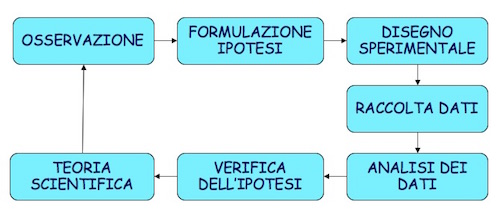
\includegraphics[width=0.75\linewidth]{_images/MSAMap} 

}

\caption{Il metodo scientifico Galileiano}\label{fig:figName11}
\end{figure}

Senza andare troppo in profondità, è importante notare due aspetti:

\begin{enumerate}
\def\labelenumi{\arabic{enumi}.}
\tightlist
\item
  il ruolo fondamentale dell'esperimento scientifico, che produce dati a supporto di ipotesi pre-esistenti;
\item
  lo sviluppo di teorie basate sui dati, che rimangono valide fino a che non si raccolgono altri dati che le confutano, facendo nascere nuove ipotesi che possono portare allo sviluppo di nuove teorie, più affidabili o più semplici.
\end{enumerate}

Insomma, l'ingrediente fondamentale di una prova scientifica è quello di essere supportata dai dati sperimentali: di fatto, non esiste scienza senza dati! Resta famoso l'aforisma ``In God we trust, all the others bring data'', attribuito all'ingegnere e statistico americano W. Edwards Deming (1900-1993), anche se pare che egli, in realtà, non l'abbia mai pronunciato.

\hypertarget{dati-buoni-e-cattivi}{%
\section{Dati `buoni' e `cattivi'}\label{dati-buoni-e-cattivi}}

Detto che la scienza si basa sui dati, bisogna anche dire che non tutti i dati sono ugualmente `buoni'. Nelle scienze biologiche, così come nelle altre scienze, è importante che i dati siano in grado di cogliere gli effetti che vogliamo studiare, senza introdurre distorsioni.

In particolare, i dati debbono essere: (1) precisi e (2) accurati. Con il termine \textbf{precisione} intendiamo due cose: la prima è relativa al numero di decimali che ci fornisce il nostro strumento di misura. E'evidente, ad esempio, come un calibro sia più preciso di un metro da sarto. Oltre a questo significato, abbastanza intuitivo, ce n'è un altro, più specificatamente legato agli esperimenti scientifici: la precisione di un dato ottenuto attraverso un processo di misurazione non è altro che la variabilità riscontrata quando la misurazione viene ripetuta più volte.

La precisione, da sola, non garantisce che i dati siano affidabili. Infatti, è anche necessario che questi corrispondano al valore vero del soggetto misurato (\textbf{accuratezza}). Può sembrare una banalità, ma proviamo a pensare ad uno strumento non tarato, che produce errori sistematici; ad esempio, pensiamo ad un gascromatografo, che restituisce sempre una concentrazione maggiorata del 20\%. Se noi ripetessimo le analisi 100 volte, in assenza di altri errori, otterremmo sempre lo stesso risultato, molto preciso, ma totalmente inaffidabile, nel senso che non riflette la concentrazione reale della soluzione in studio. L'accuratezza è addirittura più importante della precisione: infatti una misura accurata, ma imprecisa, riflette bene la realtà, anche se in modo vago. Al contrario, una misura precisa, ma inaccurata, ci porta completamente fuori strada, perché non riflette la realtà. Con linguaggio tecnico, un dato non accurato si dice `distorto' (\emph{biased}).

Per ottenere dati precisi ed accurati è necessario porre grande attenzione in relazione a tre aspetti fondamentali:

\begin{enumerate}
\def\labelenumi{\arabic{enumi}.}
\tightlist
\item
  Errore sperimentale
\item
  Variabilità dei soggetti sperimentali
\item
  Campionamento
\end{enumerate}

Vediamo ora qualche dettaglio a proposito di ciascuno di questi tre elementi.

\hypertarget{lerrore-sperimentale}{%
\subsection{L'errore sperimentale}\label{lerrore-sperimentale}}

In ogni processo di misurazione esiste sempre la possibilità di commettere due tipi di errore: \textbf{sistematico} ed \textbf{accidentale (casuale)}. L'errore sistematico è provocato da difetti intrinseci dello strumento o incapacità peculiari dell'operatore e tende a ripetersi costantemente in misure successive. Un esempio tipico è quello di una bilancia non tarata, che tende ad aggiungere 20 grammi ad ogni misura che effettuiamo. Per queste sue peculiarità, l'errore sistematico non è quantificabile e deve essere contenuto al minimo livello possibile tramite la perfetta taratura degli strumenti e l'adozione di metodi di misura rigidamente standardizzati e accettati dalla comunità scientifica mondiale. Ad esempio, a livello di laboratorio, vengono utilizzati standard di confronto, la cui misura è perfettamente nota e viene periodicamente confrontata con quella rilevabile dallo strumento stesso, per verificarne la taratura. Altro metodo utilizzato nelle procedure di accreditamento dei laboratori è rappresentato dal \emph{ring test}, dove campioni reali della matrice da misurare sono inviati a più laboratori a livello nazionale, in modo da poter confrontare le misure ottenute e valutarne la variabilità. Con un \emph{ring test}, un laboratorio può valutare la sua stessa affidabilità in confronto con laboratori simili, basandosi sull'eventuale differenza tra il risultato ottenuto e la distribuzione di quelli ottenuti in tutti gli altri laboratori valutati.

L'errore accidentale (o casuale) è invece legato a fattori variabili nel tempo e nello spazio, quali:

\begin{enumerate}
\def\labelenumi{\arabic{enumi}.}
\tightlist
\item
  malfunzionamenti accidentali dello strumento;
\item
  imprecisioni o disattenzioni casuali dell'operatore;
\item
  irregolarità dell'oggetto da misurare. Si pensi alla misurazione dell'altezza di una pianta di mais: è facile immaginare di riscontrare difficoltà legate, ad esempio, all'individuazione del punto esatto in cui inizia il culmo e del punto esatto dove termina l'infiorescenza apicale.
\end{enumerate}

L'errore accidentale è meno pericoloso di quello sistematico, poiché, essendo di natura casuale, se ripetiamo la misurazione tende a ripresentarsi con valori e segni diversi. Di conseguenza, è ragionevole pensare che le repliche, in media, possono fornire un valore accurato.

\hypertarget{la-variabilita-naturale}{%
\subsection{La variabilità naturale}\label{la-variabilita-naturale}}

Di solito non si effettua una sola misura, sia perché sussiste il dubbio di aver commesso un errore, sia perché, frequentemente, abbiamo a che fare con un collettivi di individui, più o meno numeroso. In questo caso, anche se fossimo certi di non aver commesso alcun errore di misura, dovremmo comunque considerare la naturale variabilità di tutti i fenomeni biologici, oltre a quella degli strumenti di misura. Ad esempio, pensiamo alla misurazione della produzione di granella di una certa varietà di frumento: anche ipotizzando di avere uno strumento di misura perfetto, e quindi esente da errore, la produzione mostrerebbe comunque una variabilità naturale da pianta a pianta, o da parcella a parcella, in base al patrimonio genetico, alla pedologia, al microclima, alle condizioni di coltivazione, che non possono essere standardizzate oltre ad un certo livello.

La presenza di variabilità naturale è un elemento importante; infatti non dobbiamo solo preoccuparci se il nostro strumento è in grado di intercettare la misura vera del soggetto, dobbiamo anche caratterizzare la variabilità esistente tra soggetto e soggetto e, di conseguenza, tra misura e misura, che, in qualche modo, ci permette di quantificare il livello di precisione del nostro esperimento.

\hypertarget{il-campionamento}{%
\subsection{Il campionamento}\label{il-campionamento}}

Se è vero che i collettivi sono variabili e producono misure individuali tutte diverse una dall'altra, è evidente che l'unica possibilità che abbiamo per arrivare a risultati totalmente affidabili è quella di sottoporre a misurazione tutti i soggetti del collettivo stesso. Certo, questo è possibile solo con collettivi molto piccoli, mentre, in natura, i collettivi sono talmente numerosi che la misurazione `globale' è quasi sempre improponibile.

Qual è la strada seguita dagli scienziati, quindi? E' quella di raccogliere un numero finito di misure, sufficientemente basso da essere compatibile con le umane risorse di tempo e denaro, ma sufficientemente alto da essere giudicato attendibile. Qualunque sia questo valore finito, è evidente che ci troviamo difronte solo ad un campione delle infinite misure che avremmo dovuto fare, ma che non abbiamo fatto. La domanda è: questo campione è rappresentativo o no? E' in grado di descrivere adeguatamente la realtà? E' possibile che, per errore, abbiamo trascurato alcuni dei soggetti con misure, ad esempio, molto alte e, di conseguenza, stiamo sottostimando il valore vero della misura? In altre parole: possiamo fidarci dei dati che abbiamo raccolto? Tanto per cominciare possiamo intuire che tanto maggiore è la numerosità del campione, quanto più affidabile sarà il risultato che otterremo.

Tuttavia, anche quando il campione è sufficientemente numeroso, la possibilità di raccogliere dati sbagliati è tutt'altro che remota. Gli scienziati americani Pons e Fleischmann il 23 Marzo del 1989 diffusero pubblicamente la notizia di essere riusciti a riprodurre la fusione nucleare fredda, causando elevatissimo interesse nella comunità scientifica. Purtroppo le loro misure erano viziate da una serie di problemi e il loro risultato fu clamorosamente smentito da esperimenti successivi.

\begin{figure}

{\centering 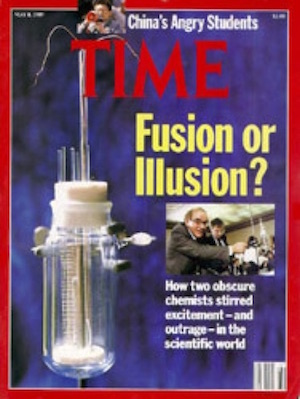
\includegraphics[width=0.5\linewidth]{_images/FalseResults} 

}

\caption{Conseguenze di un esperimento sbagliato}\label{fig:figName2}
\end{figure}

\hypertarget{scienza-metodo}{%
\section{Scienza = metodo}\label{scienza-metodo}}

Insomma, la scienza deve essere basata sui dati, che tuttavia contengono inevitabili fonti di incertezza, legate all'errore sperimentale, alla variabilità dei soggetti e al processo di campionamento. Come si può procedere in queste condizioni? Il punto fondamentale è quello di adottare metodi rigorosi, all'interno di un esperimento scientifico `valido'. In questo modo possiamo sperare di ottenere dati che, pur in presenza delle inevitabili componenti di incertezza che abbiamo già citato, sono \textbf{il più affidabili possibile}.

Come si distingue un esperimento `valido' da uno `invalido'? Tanto per cominciare, dobbiamo tener presenti due caratteristiche fondamentali, cioè:

\begin{enumerate}
\def\labelenumi{\arabic{enumi}.}
\tightlist
\item
  Replicabilità
\item
  Riproducibilità
\end{enumerate}

Un esperimento è replicabile se, quando ripetuto in condizioni assolutamente analoghe (stessi soggetti, ambiente, strumenti\ldots{}), restituisce risultati equivalenti. Per questo motivo, quando si pubblicano i risultati di un esperimento, è sempre necessario descrivere accuratamente i metodi impiegati, in modo da consentire a chiunque la verifica dei risultati.

In alcuni casi, tuttavia, questa verifica indipendente è pressoché impossibile; ad esempio, nelle scienze agronomiche, le caratteristiche genetiche e pedo-climatiche giocano un ruolo molto importante e non è facile replicare un esperimento di pieno campo esattamente nelle stesse condizioni. Per questo motivo, alcuni biostatistici distinguono la replicabilità dalla riproducibilità, definita come il grado di concordanza tra esperimenti ripetuti in condizioni diverse (diversi soggetti, diverso ambiente\ldots{}). Se la replicabilità di un esperimento non può essere dimostrata, bisogna avere almeno un'idea della sua riproducibilità, ripetendo l'esperimento in condizioni diverse e discutendo attentamente le eventuali differenze riscontrate nei risultati.

\hypertarget{elementi-fondamentali-del-disegno-sperimentale}{%
\section{Elementi fondamentali del disegno sperimentale}\label{elementi-fondamentali-del-disegno-sperimentale}}

La metodica di organizzazione di un esperimento valido prende il nome di \emph{disegno sperimentale} e le sue basi si fanno in genere risalire a Sir Ronald A. Fisher, vissuto in Inghilterra dal 7 Febbraio 1890 al 29 luglio 1962. Laureatosi nel 1912, lavora come statistico per il comune di Londra, fino a quando diviene socio della prestigiosa Eugenics Education Society di Cambridge, fondata nel 1909 da Francis Galton, cugino di Charles Darwin. Dopo la fine della guerra, Karl Pearson gli propone un lavoro presso il rinomato Galton Laboratory, ma egli non accetta a causa della profonda rivalità esistente tra lui e Pearson stesso. Nel 1919 viene assunto presso la Rothamsted Experimental Station, dove si occupa dell'elaborazione dei dati sperimentali e, nel corso dei successivi 7 anni, definisce le basi del disegno sperimentale ed elabora la sua teoria della ``analysis of variance''. Il suo libro più importante è ``The design of experiment'', del 1935. E' sua la definizione delle tre componenti fondamentali del disegno sperimentale:

\begin{enumerate}
\def\labelenumi{\arabic{enumi}.}
\tightlist
\item
  controllo degli errori;
\item
  replicazione;
\item
  randomizzazione.
\end{enumerate}

\hypertarget{controllo-degli-errori}{%
\subsection{Controllo degli errori}\label{controllo-degli-errori}}

Controllare gli errori, o, analogamente, eseguire un esperimento controllato significa fondamentalmente due cose:

\begin{enumerate}
\def\labelenumi{\arabic{enumi}.}
\tightlist
\item
  adottare provvedimenti idonei ad evitare le fonti di errore, mantenendole al livello più basso possibile (alta precisione);
\item
  agire in modo da isolare l'effetto in studio (accuratezza), evitando che si confonda con effetti casuali e di altra natura. Ad esempio, se dobbiamo confrontare due fitofarmaci, dobbiamo fare in modo che i soggetti inclusi nell'esperimento differiscano tra di loro solo per il fitofarmaco impiegato e non per altro.
\end{enumerate}

Mettere in pratica questi principi fondamentali richiede una vita di esperienza! Tuttavia, vogliamo solo sottolineare alcuni aspetti, come il rigore metodologico. È evidente che, ad esempio, se vogliamo sapere la cinetica di degradazione di un erbicida a 20 °C dovremo realizzare una prova esattamente a quella temperatura, con un erbicida uniformemente distribuito nel terreno, dentro una camera climatica capace di un controllo perfetto della temperatura. Gli strumenti dovranno essere ben tarati e sarà necessario attenersi scrupolosamente a metodi validati e largamente condivisi. Tuttavia, a proposito di rigore, non bisogna scordare quanto diceva C.F. Gauss a proposito della precisione nei calcoli, e che può essere anche riferito al rigore nella ricerca : ``\emph{Manca di mentalità matematica tanto chi non sa riconoscere rapidamente ciò che è evidente, quanto chi si attarda nei calcoli con una precisione superiore alla necessità}''

Oltre al rigore metodologico, è bene anche ricordare come un esperimento ben fatto passi sempre attraverso la giusta selezione dei soggetti sperimentali, che debbono essere omogenei, ma rappresentativi della popolazione alla quale intendiamo riferire i risultati ottenuti. Ad esempio, se si vuole ottenere un risultato riferito alla collina umbra, bisognerà scegliere parcelle di terreno omogenee, ma che rappresentano bene la variabilità pedo-climatica di quell'ambiente, né di più, né di meno.

Per concludere, vogliamo anche ricordare le cosiddette `intrusioni' cioè quegli eventi che accadono in modo inaspettato e condizionano negativamente la riuscita di un esperimento in corso. E' evidente che, ad esempio, un'alluvione, l'attacco di insetti o patogeni, la carenza idrica hanno una pesante ricaduta sulla precisione di un esperimento e sulla sua riuscita. Per quanto possibile, controllare gli errori significa anche essere capaci di prevedere le eventuali intrusioni. In un suo famoso lavoro scientifico del 1984, lo scienziato americano Stuart Hurlbert usa il termine `intrusione demoniaca' per indicare quelle intrusioni che, pur casuali, avrebbero potuto essere previste con un disegno più accurato, sottolineando in questo caso la responsabilità dello sperimentatore.

Un esempio è questo: uno sperimentatore vuole studiare l'entità della predazione dovuta alle volpi e quindi usa campi senza staccionate (dove le volpi possono entrare) e campi protetti da staccionate (e quindi liberi da volpi). Se le staccionate, essendo utilizzate dai falchi come punto d'appoggio, finiscono per incrementare l'attività predatoria di questi ultimi, si viene a creare un'intrusione demoniaca, che rende l'esperimento distorto. Il demonio, in questo caso, non è il falco, che danneggia l'esperimento, ma il ricercatore stesso, che non ha saputo prevedere una possibile intrusione.

\hypertarget{replicazione}{%
\subsection{Replicazione}\label{replicazione}}

In ogni esperimento, i trattamenti dovrebbe essere replicati su due o più unità sperimentali. Ciò permette di:

\begin{enumerate}
\def\labelenumi{\arabic{enumi}.}
\tightlist
\item
  dimostrare che i risultati sono replicabili (ma non è detto che siano riproducibili!);
\item
  rassicurare che eventuali circostanze aberranti casuali non abbiano provocato risultati distorti;
\item
  misurare la precisione dell'esperimento, come variabilità di risposta tra repliche trattate nello stesso modo;
\item
  incrementare la precisione dell'esperimento (più sono le repliche più l'esperimento è preciso, perché si migliora la stima della caratteristica misurata, diminuendo l'incertezza).
\end{enumerate}

Per poter essere utili, le repliche debbono essere indipendenti, cioè debbono \textbf{aver subito tutte le manipolazioni necessarie per l'allocazione del trattamento in modo totalmente indipendente l'una dall'altra}. Le manipolazioni comprendono tutte le pratiche necessarie, come ad esempio la preparazione delle soluzioni, la diluizione dei prodotti, ecc..

La manipolazione indipendente è fondamentale, perché in ogni parte del processo di trattamento possono nascondersi errori più o meno grandi, che possono essere riconosciuti solo se colpiscono in modo casuale le unità sperimentali. Se la manipolazione è, anche solo in parte, comune, questi errori colpiscono tutte le repliche allo stesso modo, diventano sistematici e quindi non più riconoscibili. Di conseguenza, si inficia l'accuratezza dell'esperimento. Quando le repliche non sono indipendenti, si parla di \textbf{pseudorepliche}, contrapposte alle \textbf{repliche vere}.

Il numero di repliche dipende dal tipo di esperimento: più sono e meglio è, anche se è necessario trovare un equilibrio accettabile tra precisione e costo dell'esperimento. Nella sperimentazione di campo, due repliche sono poche, tre appena sufficienti, quattro costituiscono la situazione più comune, mentre un numero maggiore di repliche è abbastanza raro, non solo per la difficoltà di seguire l'esperimento, ma anche perché aumentano la dimensione della prova e, di conseguenza, la variabilità del terreno.

\hypertarget{randomizzazione}{%
\subsection{Randomizzazione}\label{randomizzazione}}

L'indipendenza di manipolazione non garantisce da sola un esperimento corretto. Infatti potrebbe accadere che le caratteristiche innate dei soggetti, o una qualche `intrusione' influenzino in modo sistematico tutte le unità sperimentali trattate nello stesso modo, così da confondersi con l'effetto del trattamento. Un esempio banale è che potremmo somministrare un farmaco a quattro soggetti in modo totalmente indipendente, ma se i quattro soggetti fossero sistematicamente più alti di quelli non trattati finiremmo per confondere una caratteristica innata con l'effetto del farmaco. Oppure, se le piante di una certa varietà di sorgo si trovassero tutte più vicine alla scolina rispetto a quelle di un'altra varietà, potrebbero essere più danneggiate dal ristagno idrico, il cui effetto si confonderebbe con quello del trattamento stesso.

Questi problemi sono particolarmente insidiosi e si nascondono anche dietro ai particolari apparentemente più insignificanti. La randomizzazione è l'unico sistema per evitare, o almeno rendere molto improbabile, la confusione dell'effetto del trattamento con fattori casuali e/o comunque diversi dal trattamento stesso. La randomizzazione si declina in vari modi:

\begin{enumerate}
\def\labelenumi{\arabic{enumi}.}
\tightlist
\item
  allocazione casuale del trattamento alle unità sperimentali. Gli esperimenti che prevedono l'allocazione del trattamento sono detti `manipolativi' o `disegnati'.
\item
  A volte l'allocazione del trattamento non è possibile o non è etica. Se volessimo studiare l'effetto delle cinture di sicurezza nell'evitare infortuni gravi, non potremmo certamente provocare incidenti deliberati. In questo caso la randomizzazione è legata alla scelta casuale di soggetti che sono `naturalmente' trattati. Esperimenti di questi tipo, si dicono \textbf{osservazionali}. Un esempio è la valutazione dell'effetto dell'inquinamento con metalli pesanti nella salute degli animali: ovviamente non è possibile, se non su piccola scala, realizzare il livello di inquinamento desiderato e, pertanto, dovremo scegliere soggetti che sono naturalmente sottoposti a questo genere di inquinamento, magari perché vivono vicino a zone industriali.
\item
  Se i soggetti sono immobili, la randomizzazione ha anche una connotazione legata alla disposizione spaziale e/o temporale casuale.
\end{enumerate}

L'assegnazione casuale del trattamento, o la selezione casuale dei soggetti trattati, fanno si che tutti i soggetti abbiano la stessa probabilità di ricevere qualunque trattamento oppure qualunque intrusione casuale. In questo modo, la probabilità che tutte le repliche di un trattamento abbiano qualche caratteristica innata o qualche intrusione comune che li penalizzi/avvantaggi viene minimizzata. Di conseguenza, confondere l'effetto del trattamento con variabilità casuale (`confounding'), anche se teoricamente possibile, diviene altamente improbabile.

\hypertarget{esperimenti-invalidi}{%
\subsection{Esperimenti invalidi}\label{esperimenti-invalidi}}

A questo punto dovrebbe essere chiaro che un esperimento valido deve essere controllato, replicato e randomizzato: la mancanza anche di uno solo di questi elementi pone dubbi ragionevoli sull'affidabilità dei risultati. In particolare, gli esperimenti `invalidi' sono caratterizzati da:

\begin{enumerate}
\def\labelenumi{\arabic{enumi}.}
\tightlist
\item
  Cattivo controllo degli errori
\item
  Fondati sospetti di confounding
\item
  Mancanza di repliche vere
\item
  Confusione tra repliche vere e pseudo-repliche
\item
  Mancanza di randomizzazione
\item
  Presenza di vincoli alla randomizzazione, trascurati in fase di analisi.
\end{enumerate}

Le conseguenze di queste problematiche sono abbastanza diverse.

\hypertarget{cattivo-controllo-degli-errori}{%
\subsubsection{Cattivo controllo degli errori}\label{cattivo-controllo-degli-errori}}

Bisogna verificare se il problema è relativo a questioni come la mancanza di scrupolosità, l'uso di soggetti poco omogenei o di un ambiente poco omogeneo, o altri aspetti che inficiano solo la precisione, ma non l'accuratezza dell'esperimento. In questo caso, l'esperimento è ancora valido (accurato), ma la bassa precisione probabilmente impedirà di trarre conclusioni forti. Quindi, un esperimento impreciso si `elimina' da solo, perché sarà inconclusivo. Di questi esperimenti bisogna comunque diffidare, soprattutto quando siano pianificati per mostrare l'assenza di differenze tra due trattamenti alternativi. Mostrare l'assenza di differenze è facile: basta fare male un esperimento, in modo che vi sia un alto livello di incertezza e quindi l'evidenza scientifica sia molto debole.

Diversa è la situazione in cui un cattivo controllo degli errori, ad esempio l'adozione di metodi sbagliati, porta a mancanza di accuratezza, cioè a risultati che non riflettono la realtà (campionamento sbagliato, ad esempio; oppure strumenti non tarati; impiego di metodi non validati e/o non accettabili). In questo caso venendo a mancare l'accuratezza, l'esperimento deve essere rigettato, in quanto non fornisce informazioni realistiche.

\hypertarget{confounding-e-correlazione-spuria}{%
\subsubsection{`Confounding' e correlazione spuria}\label{confounding-e-correlazione-spuria}}

Abbiamo appena menzionato il problema fondamentale della ricerca, cioè il \textbf{confounding}, vale a dire la confusione tra l'effetto del trattamento e un qualche altro effetto casuale, legato alle caratteristiche innate del soggetto o a qualche intrusione più o meno `demoniaca'. Abbiamo detto che non possiamo mai avere la certezza dell'assenza di confounding, ma abbiamo anche detto che l'adozione di una pratica sperimentale corretta ne minimizza la probabilità.

Chiaramente, rimangono dei rischi che sono tipici di situazioni nelle quali il controllo adottato non è perfetto, come capita, ad esempio, negli esperimenti osservazionali. In questo ambito è piuttosto temuta la cosiddetta `correlazione spuria', una forma di confounding casuale per cui due variabili variano congiuntamente (sono direttamente o inversamente proporzionali), ma in modo del tutto casuale. Esistono, ad esempio, dati che mostrano una chiara correlazione tra le vendite di panna acida e le morti per incidenti in motocicletta. Chiaramente, non esistono spiegazioni scientifiche per questo effetto, che è, ovviamente, del tutto casuale. Il problema è che questa correlazione spuria non è sempre così semplice da rintracciare.

\begin{figure}

{\centering 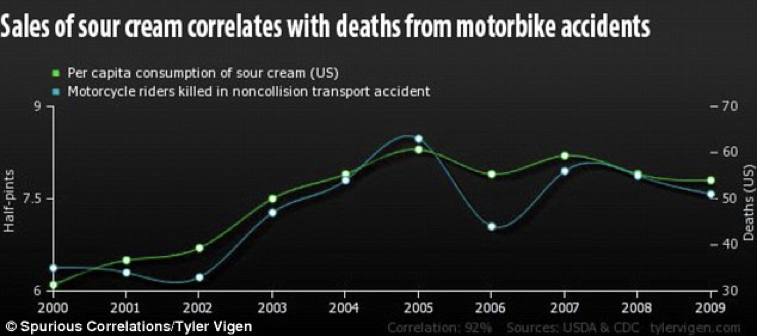
\includegraphics[width=0.9\linewidth]{_images/PannaAcida} 

}

\caption{Esempio di correlazione spuria}\label{fig:figName22}
\end{figure}

A volte il confounding non è casuale, ma è legato ad una variabile esterna che si agisce all'insaputa dello sperimentatore. Ad esempio, è stato osservato che il tasso di crimini è più alto nelle città che hanno più chiese. La spiegazione di questo paradosso sta nel fatto che esiste un `confounder', cioè l'ampiezza della popolazione. Nelle grandi città si riscontrano sia una maggiore incidenza criminale, sia un grande numero di chiese. In sostanza, la popolazione determina sia l'elevato numero di chiese che l'elevato numero di crimini, ma queste ultime due variabili non sono legate tra loro da una relazione causa-effetto (A implica B e A implica C, ma B non implica C).

Il confounding non casuale è spesso difficile da evidenziare, soprattutto se le correlazioni misurate sono spiegabili. Inoltre, non è eliminabile con un'accurata randomizzazione, ma solo con l'esecuzione di un esperimento totalmente controllato, nel quale ci si preoccupa di rilevare tutte le variabili necessarie per spiegare gli effetti riscontrati. Di questo è importante tener conto soprattutto negli esperimenti osservazionali, dove il controllo è sempre più difficile e meno completo.

\hypertarget{pseudo-repliche-e-randomizzazione-poco-attenta}{%
\subsubsection{Pseudo-repliche e randomizzazione poco attenta}\label{pseudo-repliche-e-randomizzazione-poco-attenta}}

Per evidenziare questi problemi e comprendere meglio la differenza tra un esperimento corretto e uno non corretto, è utilissima la classificazione fatta da Hurlbert (1984), che riportiamo di seguito.

\begin{figure}

{\centering 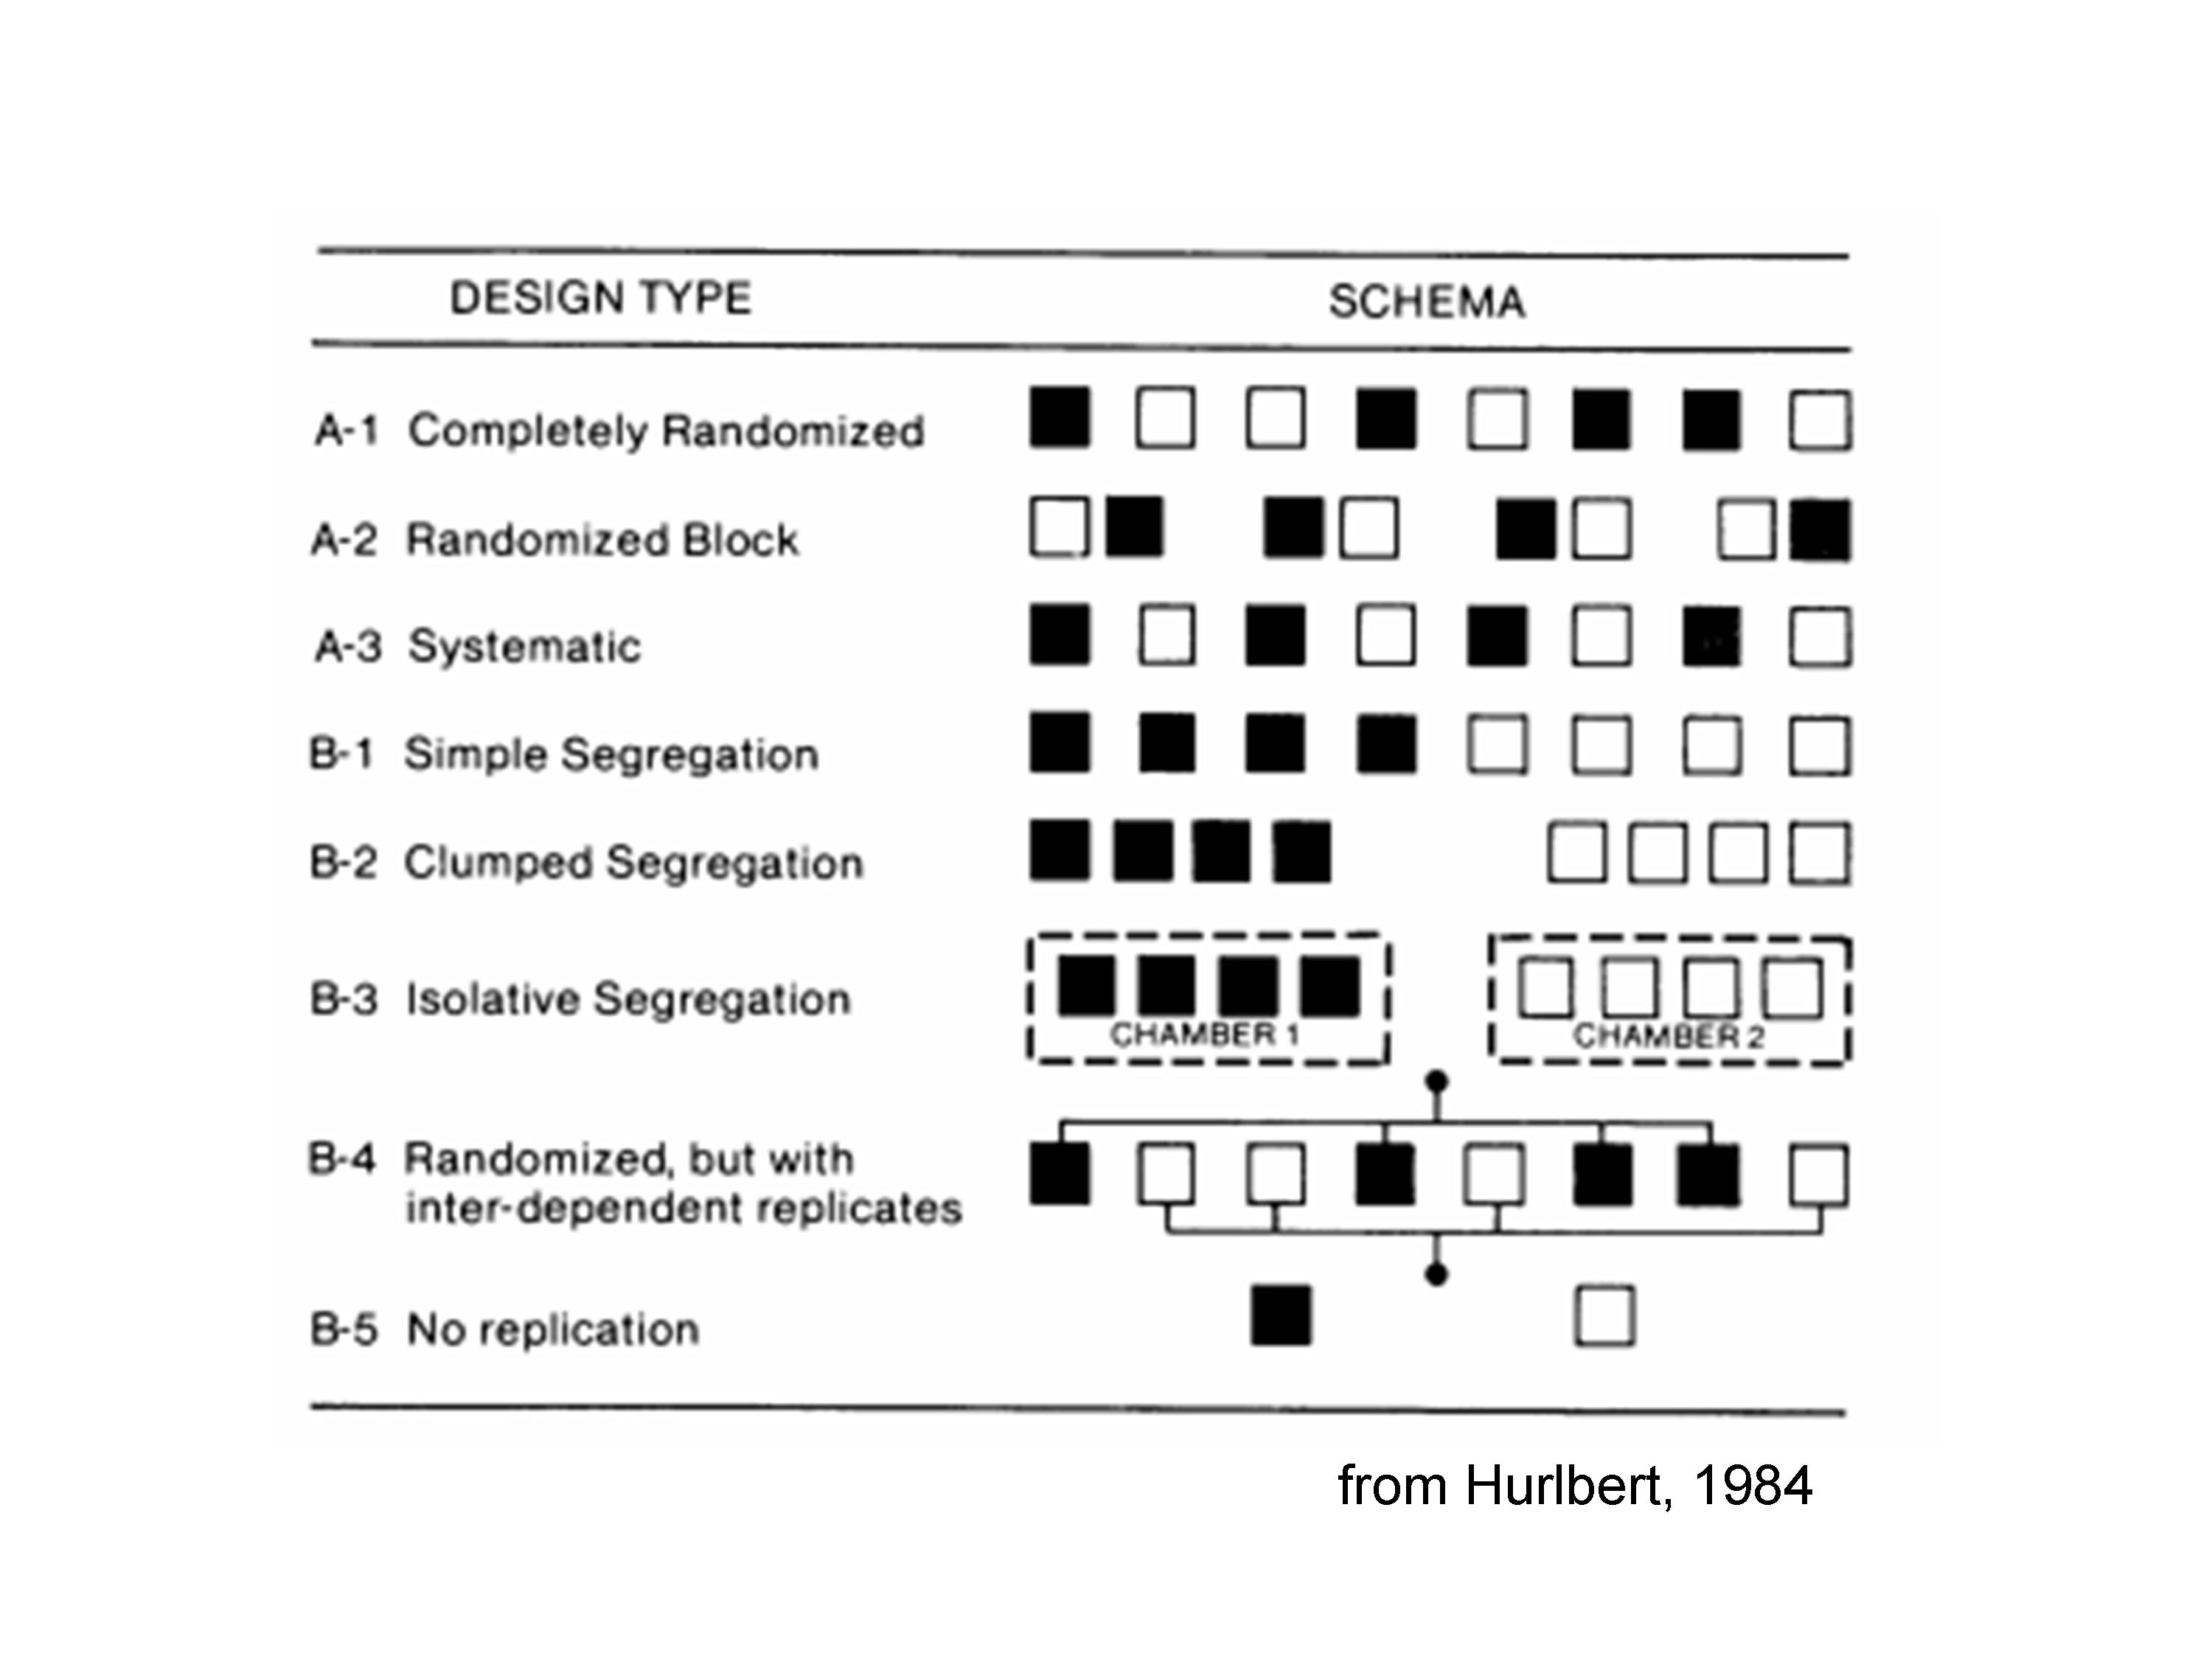
\includegraphics[width=0.9\linewidth]{_images/Randomisation} 

}

\caption{Indicazioni per una corretta randomizzazione (Hurlbert, 1984)}\label{fig:figName23}
\end{figure}

Vengono mostrati 8 soggetti, sottoposti a due trattamenti (bianco e nero), con 8 disegni sperimentali diversi.

Il disegno A1 è corretto, in quanto si tratta di un esperimento completamente randomizzato. Ugualmente, è valido il disegno A2, nel quale le unità sperimentali sono state divise in quattro gruppi omogenei e sono state trattate in modo randomizzato all'interno di ogni gruppo.

Il disegno A3 è quantomeno `sospetto': vi sono repliche vere, ma l'allocazione dei trattamenti non è randomizzata ed avviene con un processo sistematico per il quale `nero' e `bianco' si alternano. Cosa succederebbe se vi fosse un gradiente di fertilità decrescente da destra verso sinistra? Le unità nere sarebbero avvantaggiate rispetto alle bianche! Insomma, rimangono sospetti di confounding, a meno che non si sia assolutamente certi dell'assenza di gradienti, come capita ad esempio se all'interno dei blocchi, dobbiamo creare una sequenza spazio-temporale. Vediamo tre esempi:

\begin{enumerate}
\def\labelenumi{\arabic{enumi}.}
\tightlist
\item
  ho quattro piante e, per ogni pianta, voglio confrontare un ramo basso con uno alto: è evidente che i due trattamenti sono sempre ordinati in modo sistematico (basso prima di alto).
\item
  Dobbiamo valutare l'effetto di fitofarmaci somministrati in due epoche diverse (accestimento e inizio-levata); anche qui non possiamo randomizzare, giacché un'epoca precede sempre l'altra.
\item
  Dobbiamo confrontare la presenza di residui di un fitofarmaco a due profondità e non possiamo randomizzare, perché una profondità precede sempre l'altra nello spazio.
\end{enumerate}

In queste situazioni l'esperimento rimane valido, anche se la randomizzazione segue un processo sistematico e non casuale.

Il disegno B1 è usualmente invalido: non vi è randomizzazione e ciò massimizza i problemi del disegno A3: la separazione delle unità sperimentali `bianche' e `nere' non consente una valutazione adeguata dell'effetto del trattamento, che è confuso con ogni potenziale differenza tra la parte destra e la sinistra dell'ambiente in cui la sperimentazione viene eseguita. Ovviamente, la separazione può essere non solo spaziale, ma anche temporale. Anche in questo caso diamo alcuni esempi in cui una situazione come quella descritta in B1 è valida:

\begin{enumerate}
\def\labelenumi{\arabic{enumi}.}
\tightlist
\item
  Vogliamo confrontare la produzione in pianura e in collina. Ovviamente dobbiamo scegliere campioni in due situazioni fisicamente separate
\item
  Vogliamo confrontare la pescosità di due laghetti
\item
  Vogliamo confrontare la produttività di due campi contigui.
\end{enumerate}

Queste situazioni sono valide, anche se con una restrizione: non siamo in grado di stabilire a chi debba essere attribuito l'effetto. Ad esempio, per la prima situazione, pianura e collina possono dare produzioni diverse per il suolo diverso, il clima diverso, la precessione colturale diversa o un qualunque altro elemento che differenzi le due località.

Il disegno B2 è analogo al disegno B1, ma il problema è più grave, perché la separazione fisica è più evidente. Questo disegno è totalmente sbagliato, a meno che non siamo specificatamente interessati all'effetto località (vedi sopra).

Il disegno B3 è analogo al disegno B2, ma costituisce una situazione molto frequente nella pratica scientifica. Immaginiamo infatti di voler confrontare la germinazione dei semi a due temperature diverse, utilizzando due camere climatiche e mettendo, in ognuna di esse, quattro capsule Petri identiche. In questa situazione, l'effetto temperatura è totalmente confuso con l'effetto `camera climatica (località)' e risente di ogni malfunzionamento relativo ad una sola delle due camere. Inoltre, le unità sperimentali con lo stesso trattamento di temperature non sono manipolate in modo indipendente, dato che condividono la stessa camera climatica. Di conseguenza, non si può parlare di repliche vere, bensì di \textbf{pseudorepliche}.

Altri esempi di \textbf{pseudorepliche} sono schematizzati con il codice B4. Ad esempio:

\begin{enumerate}
\def\labelenumi{\arabic{enumi}.}
\tightlist
\item
  trattare piante in vaso ed analizzare in modo indipendente i singoli individui invece che tutto il vaso;
\item
  trattare una parcella di terreno e prelevare da essa più campioni, analizzandoli separatamente;
\item
  trattare una capsula Petri ed analizzare separatamente i semi germinati al suo interno.
\end{enumerate}

Questi disegni, in assenza di repliche vere aggiuntive non sono da considerarsi validi. Ad esempio, se io ho due vasetti trattati in modo totalmente indipendente e da ciascuno di essi prelevo due piante e le analizzo separatamente, il disegno è caratterizzato da due repliche vere e due pseudorepliche per ogni replica ed è, pertanto, valido.

Il disegno B5 è invece evidentemente invalido, per totale mancanza di repliche.

\hypertarget{scienza-e-falsificabilita}{%
\section{Scienza e falsificabilità}\label{scienza-e-falsificabilita}}

Certo è che, per quanto detto in precedenza, il fatto che i dati provengano da un processo di campionamento impedisce, di fatto, di ottenere un'affidabilità totale. Cosa succederebbe se ripetessimo l'esperimento?

Insomma, bisogna fare alcune considerazioni, riportate di seguito:

\begin{enumerate}
\def\labelenumi{\arabic{enumi}.}
\tightlist
\item
  in primo luogo si dovrà accettare il fatto che, contrariamente a quanto si potrebbe o vorrebbe credere, non esistono prove scientifiche totalmente certe, ma l'incertezza è un elemento intrinseco della scienza.
\item
  In secondo luogo si dovranno utilizzare gli strumenti della statistica necessari per quantificare l'incertezza residua, che dovrà essere sempre riportata a corredo dei risultati di ogni esperimento scientifico.
\item
  Ogni risultato sarà quindi valutato dalla comunità scientifica sullo sfondo della sua incertezza, seguendo alcune regole di natura probabilistica che consentono di stabilire se la prova scientifica è sufficientemente forte per essere considerata tale.
\end{enumerate}

È chiaro comunque che ogni esperimento può essere smentito. Questo non è un problema: la scienza è pronta a considerare una prova scientifica valida fino a che non si raccolgono dati altrettanto affidabili che la confutino. In questo caso, si abbandona la teoria confutata e si abbraccia la nuova. L'abbandono può anche non essere totale: ad esempio la teoria gravitazionale di Newton è ancora oggi valida per molto situazioni pratiche, anche se è stata abbandonata in favore della teoria della relatività, che spiega meglio il moto dei corpi ad altissime velocità.

In effetti, la scienza considera sempre con attenzione il principio del rasoio di Occam, per il quale si accetta sempre la teoria più semplice per interpretare una dato fenomeno, riservando le teorie più complesse alle situazioni più difficili, che giustificano tale livello di complessità.

\hypertarget{chi-valuta-se-un-esperimento-e-attendibile}{%
\section{Chi valuta se un esperimento è attendibile?}\label{chi-valuta-se-un-esperimento-e-attendibile}}

Quanto detto finora vorrebbe chiarire come il punto centrale della scienza non è la certezza delle teorie, bensì il metodo che viene utilizzato per definirle. Ognuno di noi è quindi responsabile di verificare che le informazioni in suo possesso siano `scientificamente' attendibili, cioè ottenute con un metodo sperimentale adeguato. Il fatto è che non sempre siamo in grado di compiere questa verifica, perché non abbiamo strumenti `culturali' adeguati, se non nel ristretto ambito delle nostre competenze professionali. Come fare allora?

L'unica risposta accettabile è quella di controllare l'attendibilità delle fonti di informazione. In ambito biologico, le riviste autorevoli sono caratterizzate dal procedimento di `\emph{peer review}', nel quale i manoscritti scientifici, prima della pubblicazione, sono sottoposti ad un comitato editoriale ed assegnati ad un `editor', il quale legge il lavoro e contemporaneamente lo invia a due o tre scienziati anonimi e particolarmente competenti in quello specifico settore scientifico (\emph{reviewers} o revisori).

I revisori, insieme all'\emph{editor}, compiono un attento lavoro di esame e stabiliscono se l'evidenza scientifica presentata è sufficientemente `forte'. Le eventuali critiche vengono presentate all'autore, che è tenuto a rispondere in modo convincente, anche ripetendo gli esperimenti se necessario. Il processo richiede spesso interi mesi ed è abbastanza impegnativo per uno scenziato. E' piuttosto significativa l'immagine presentata in \href{http://scienceblogs.com/startswithabang/2013/06/07/the-4-jobs-of-a-referee-in-peer-review/}{scienceBlog.com}, che allego qui.

\begin{figure}

{\centering 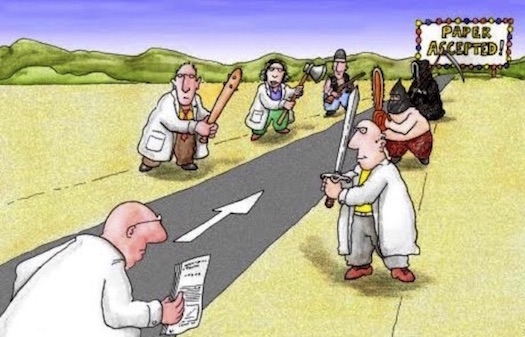
\includegraphics[width=0.75\linewidth]{_images/PeerReview} 

}

\caption{Il processo di peer review}\label{fig:figName3}
\end{figure}

In sostanza il meccanismo di \emph{peer review} porta a rigettare un lavoro scientifico in presenza di qualunque ragionevole dubbio metodologico. Desideriamo sottolineare che abbiamo parlato di dubbio metodologico, dato che il dubbio sul risultato non può essere allontanato completamente e i reviewer controlleranno solo che il rischio di errore sia al disotto della soglia massima arbitrariamente stabilita (di solito pari al 5\%).
Questo procedimento, se effettuato con competenza, dovrebbe aiutare a separare la scienza dalla pseudo-scienza e, comunque, ad eliminare la gran parte degli errori metodologici dai lavori scientifici.

\hypertarget{conclusioni}{%
\section{Conclusioni}\label{conclusioni}}

In conclusione, possiamo ripartire dalla domanda iniziale: ``Che cosa è la scienza?'', per rispondere che è scienza tutto ciò che è supportato da dati che abbiano passato il vaglio della \emph{peer review}, dimostrando di essere stati ottenuti con un procedimento sperimentale privo di vizi metodologici e di essere sufficientemente affidabili in confronto alle fonti di incertezza cui sono associati.

Qual è il \emph{take-home message} di questo capitolo? Fidatevi solo delle riviste scientifiche attendibili, cioè quelle che adottano un serio processo di \emph{peer review} prima della pubblicazione.

\begin{center}\rule{0.5\linewidth}{\linethickness}\end{center}

\hypertarget{per-approfondire-un-po}{%
\section{Per approfondire un po'\ldots{}}\label{per-approfondire-un-po}}

\begin{enumerate}
\def\labelenumi{\arabic{enumi}.}
\tightlist
\item
  Fisher, Ronald A. (1971) {[}1935{]}. The Design of Experiments (9th ed.). Macmillan. ISBN 0-02-844690-9.
\item
  Hurlbert, S., 1984. Pseudoreplication and the design of ecological experiments. Ecological Monographs, 54, 187-211
\item
  Kuehl, R. O., 2000. Design of experiments: statistical principles of research design and analysis. Duxbury Press (CHAPTER 1)
\end{enumerate}

\hypertarget{progettare-un-esperimento}{%
\chapter{Progettare un esperimento}\label{progettare-un-esperimento}}

Qualunque sia l'ambito scientifico, nella progettazione di un esperimento possiamo individuare alcune fasi fondamentali, che proviamo ad elencare:

\begin{enumerate}
\def\labelenumi{\arabic{enumi}.}
\tightlist
\item
  individuazione del background (ricerca bibliografica)
\item
  definizione dell'ipotesi scientifica e dell'obiettivo;
\item
  identificazione dei fattore/i sperimentale/i;
\item
  identificazione dei soggetti sperimentali e delle repliche;
\item
  identificazione delle variabili da rilevare;
\item
  allocazione dei trattamenti;
\item
  impianto dell'esperimento.
\end{enumerate}

Nell'analizzare questi aspetti, faremo riferimento ad alcuni esempi pratici, che verranno presentati tra poco.

\hypertarget{ipotesi-scientifica-rightarrow-obiettivo-dellesperimento}{%
\section{\texorpdfstring{Ipotesi scientifica \(\rightarrow\) obiettivo dell'esperimento}{Ipotesi scientifica \textbackslash{}rightarrow obiettivo dell'esperimento}}\label{ipotesi-scientifica-rightarrow-obiettivo-dellesperimento}}

Trascurando la parte di ricerca bibliografica, che è pur fondamentale, nel metodo scientifico galileiano, il punto di partenza di un esperimento è l'\textbf{ipotesi scientifica}, che determina l'obiettivo dell'esperimento. Si tratta del passaggio fondamentale dal quale dipende in modo logico tutto il lavoro successivo. Gli obiettivi debbono essere:

\begin{enumerate}
\def\labelenumi{\arabic{enumi}.}
\tightlist
\item
  rilevanti
\item
  chiaramente definiti;
\item
  specifici;
\item
  misurabili;
\item
  raggiungibili/realistici;
\item
  temporalmente organizzati.
\end{enumerate}

Il rischio che si corre con obiettivi mal posti è quello di eseguire una ricerca dispersiva, con raccolta di dati non necessari e/o mancanza di dati fondamentali, con costi più elevati del necessario e un uso poco efficiente delle risorse. In genere, prima si definisce un obiettivo generale, seguito da uno o più obiettivi specifici, in genere proiettati su un più breve spazio temporale e che possono essere visti anche come le fasi necessarie per raggiungere l'obiettivo generale.

\hypertarget{identificazione-dei-fattori-sperimentali}{%
\section{Identificazione dei fattori sperimentali}\label{identificazione-dei-fattori-sperimentali}}

Dopo aver definito l'obiettivo di un esperimento, è necessario chiarire esattamente gli stimoli a cui saranno sottoposte le unità sperimentali. Uno `stimolo' sperimentale prende il nome di \textbf{fattore sperimentale}, che può avere più \textbf{livelli}. I livelli del fattore sperimentale prendono il nome di \textbf{trattamenti (o tesi) sperimentali}.

\hypertarget{esperimenti-multifattoriali}{%
\subsection{Esperimenti (multi)fattoriali}\label{esperimenti-multifattoriali}}

In alcuni casi è necessario inserire in prova più di un fattore sperimentale. In questo caso si parla di esperimenti \textbf{fattoriali}, che possono essere \textbf{incrociati (crossed)} quando sono presenti in prova tutte le possibili combinazioni dei livelli di ogni fattore, oppure di esperimenti \textbf{innestati (nested)} quando i livelli di un fattore cambiano al cambiare dei livelli dell'altro.

Ad esempio:

\begin{enumerate}
\def\labelenumi{\arabic{enumi}.}
\tightlist
\item
  Immaginiamo di voler studiare due fattori sperimentali: la varietà di girasole (tre livelli: A, B e C) e la concimazione (2 livelli: pollino e urea). Abbiamo quindi 6 possibili trattamenti (combinazioni): A-pollina, A-urea, B-pollina, B-urea, C-pollina e C-urea. Il disegno è completamente incrociato.
\item
  Immaginiamo di voler confrontare due specie in agricoltura biologica (orzo e triticale), con tre varietà ciascuna (A, B e C per orzo, D, E e F per triticale). Anche in questo caso abbiamo sei trattamenti: orzo-A, orzo-B, orzo-C, triticale-D, triticale-E e triticale-F, ma il disegno è innestato, perché per il fattore sperimentale `varietà' i livelli cambiano a seconda dei livelli del fattore `specie'.
\end{enumerate}

\hypertarget{aggiungere-un-controllo}{%
\subsection{Aggiungere un controllo?}\label{aggiungere-un-controllo}}

In alcuni casi si pone il problema di inserire in prova un trattamento che funga da riferimento per tutti gli altri. In questi casi si parla comunemente di \textbf{controllo} o \textbf{testimone}, che può essere

\begin{enumerate}
\def\labelenumi{\arabic{enumi}.}
\tightlist
\item
  non sottoposto a trattamento
\item
  trattato con placebo
\item
  trattato secondo le modalità usuali di riferimento
\end{enumerate}

Ad esempio, è usuale includere in un confronto varietale, la varietà di riferimento, che ci consente di capire se le prestazione delle nuove varietà sono effettivamente interessanti oppure no.

Per quello che riguarda invece gli studi tossicologici, è evidente l'importanza di includere un controllo non trattato. Il placebo è una preparazione che contiene tutti gli ingredienti della formulazione attiva, meno che il principio attivo. Il placebo si rende necessario in una serie di circostanze, ad esempio:

\begin{enumerate}
\def\labelenumi{\arabic{enumi}.}
\tightlist
\item
  quando il soggetto è influenzabile e può reagire alla semplice idea di essere stato trattato (effetto placebo)
\item
  quando i co-formulanti o la soluzione impiegata per veicolare il principio attivo possono mostrare un effetto sul soggetto
\end{enumerate}

\hypertarget{scelta-delle-unita-sperimentali}{%
\section{Scelta delle unità sperimentali}\label{scelta-delle-unita-sperimentali}}

In primo luogo dovremo scegliere la cosiddetta \textbf{cornice di campionamento}, cioè la popolazione di soggetti ai quali si vogliono riferire i risultati ottenuti. La scelta della cornice di campionamento è fondamentale: devo effettuare un esperimento valido per l'Italia centrale, per una località particolare, per tutta Italia? Devo fare un esperimento che riguarda una stalla in particolare o tutte le stalle dove si allevano bovini? Di quale razza? Ad esempio, se vogliamo determinare la produttività delle varietà di tabacco e la loro adattabilità alle condizioni umbre, la cornice di campionamento sarà la media e alta valle del Tevere ed i risultati ottenuti non potranno essere estesi, ad esempio, al tavoliere delle Puglie, se non con la necessaria prudenza.

E' superfluo dire che, nell'ambito della cornice di campionamento, il campione deve essere prescelto in modo da essere rappresentativo, altrimenti l'esperimento è invalido. Dare indicazioni su come si possa assicurare la rappresentatività del campione è impossibile, in quanto ciò dipende dalla tipologia di esperimento. Il campionamento è fondamentale nelle scienze sociali, dove vengono applicate tecniche particolari, come il campionamento randomizzato (completamente casuale), quello stratificato (che avviene all'interno di strati omogenei della popolazione), quello sistematico (es. prendo il primo soggetto che incontro e poi ne prendo uno ogni dieci), ecc.. Chi fosse interessato può reperire informazioni nei testi indicati in fondo al capitolo. Nelle scienze agrarie e biologiche, il campionamento si giova di metodologie meno `raffinate' e spesso si prendono i soli soggetti disponibili (le parcelle di un campo sperimentale o gli animali della stalla del Dipartimento in cui si opera\ldots{}), purché siano rappresentativi di una certa popolazione ben definita.

Per quanto riguarda la sperimentazione di pieno campo, l'omogeneità dell'ambiente è fondamentale per aumentare la precisione dell'esperimento, cosa che si consegue, innanzitutto, con la scelta dell'appezzamento giusto. Questa scelta è particolarmente delicata ed è guidata soprattutto dall'esperienza, tenendo conto anche di aspetti come la facilità di accesso e la vicinanza di strutture (laboratori, capannoni\ldots{}), che consentano un'accurata esecuzione degli eventuali prelievi. Oltre a scegliere correttamente l'appezzamento, è importante anche porre in atto alcune operazioni che consentano di incrementare ulteriormente l'omogenità dell'appezzamento prescelto. Ad esempio, talvolta si usa far precedere la prova da una coltura di `omogeneizzazione', ad esempio avena, che è molto avida di azoto e lascia nel terreno poca fertilità residua. Oppure un prato di erba medica, che, grazie agli sfalci periodici, lascia il terreno libero da piante infestanti.

\hypertarget{unita-sperimentali-in-campo-le-parcelle}{%
\subsection{Unità sperimentali in campo: le parcelle}\label{unita-sperimentali-in-campo-le-parcelle}}

Solitamente, nella ricerca biologica, le unità sperimentali sono chiaramente definite: un animale, una persona, un insetto, un'aliquota di terreno. In genere, qualunque esse siano, debbono essere chiaramente identificate prima di procedere all'allocazione dei trattamenti.

Nella sperimentazione di pieno campo, le unità sperimentali sono dette \textbf{parcelle} e sono un pezzetto di terreno, di varia forma e dimensione (Figura \ref{fig:figName21} ).

\begin{figure}

{\centering 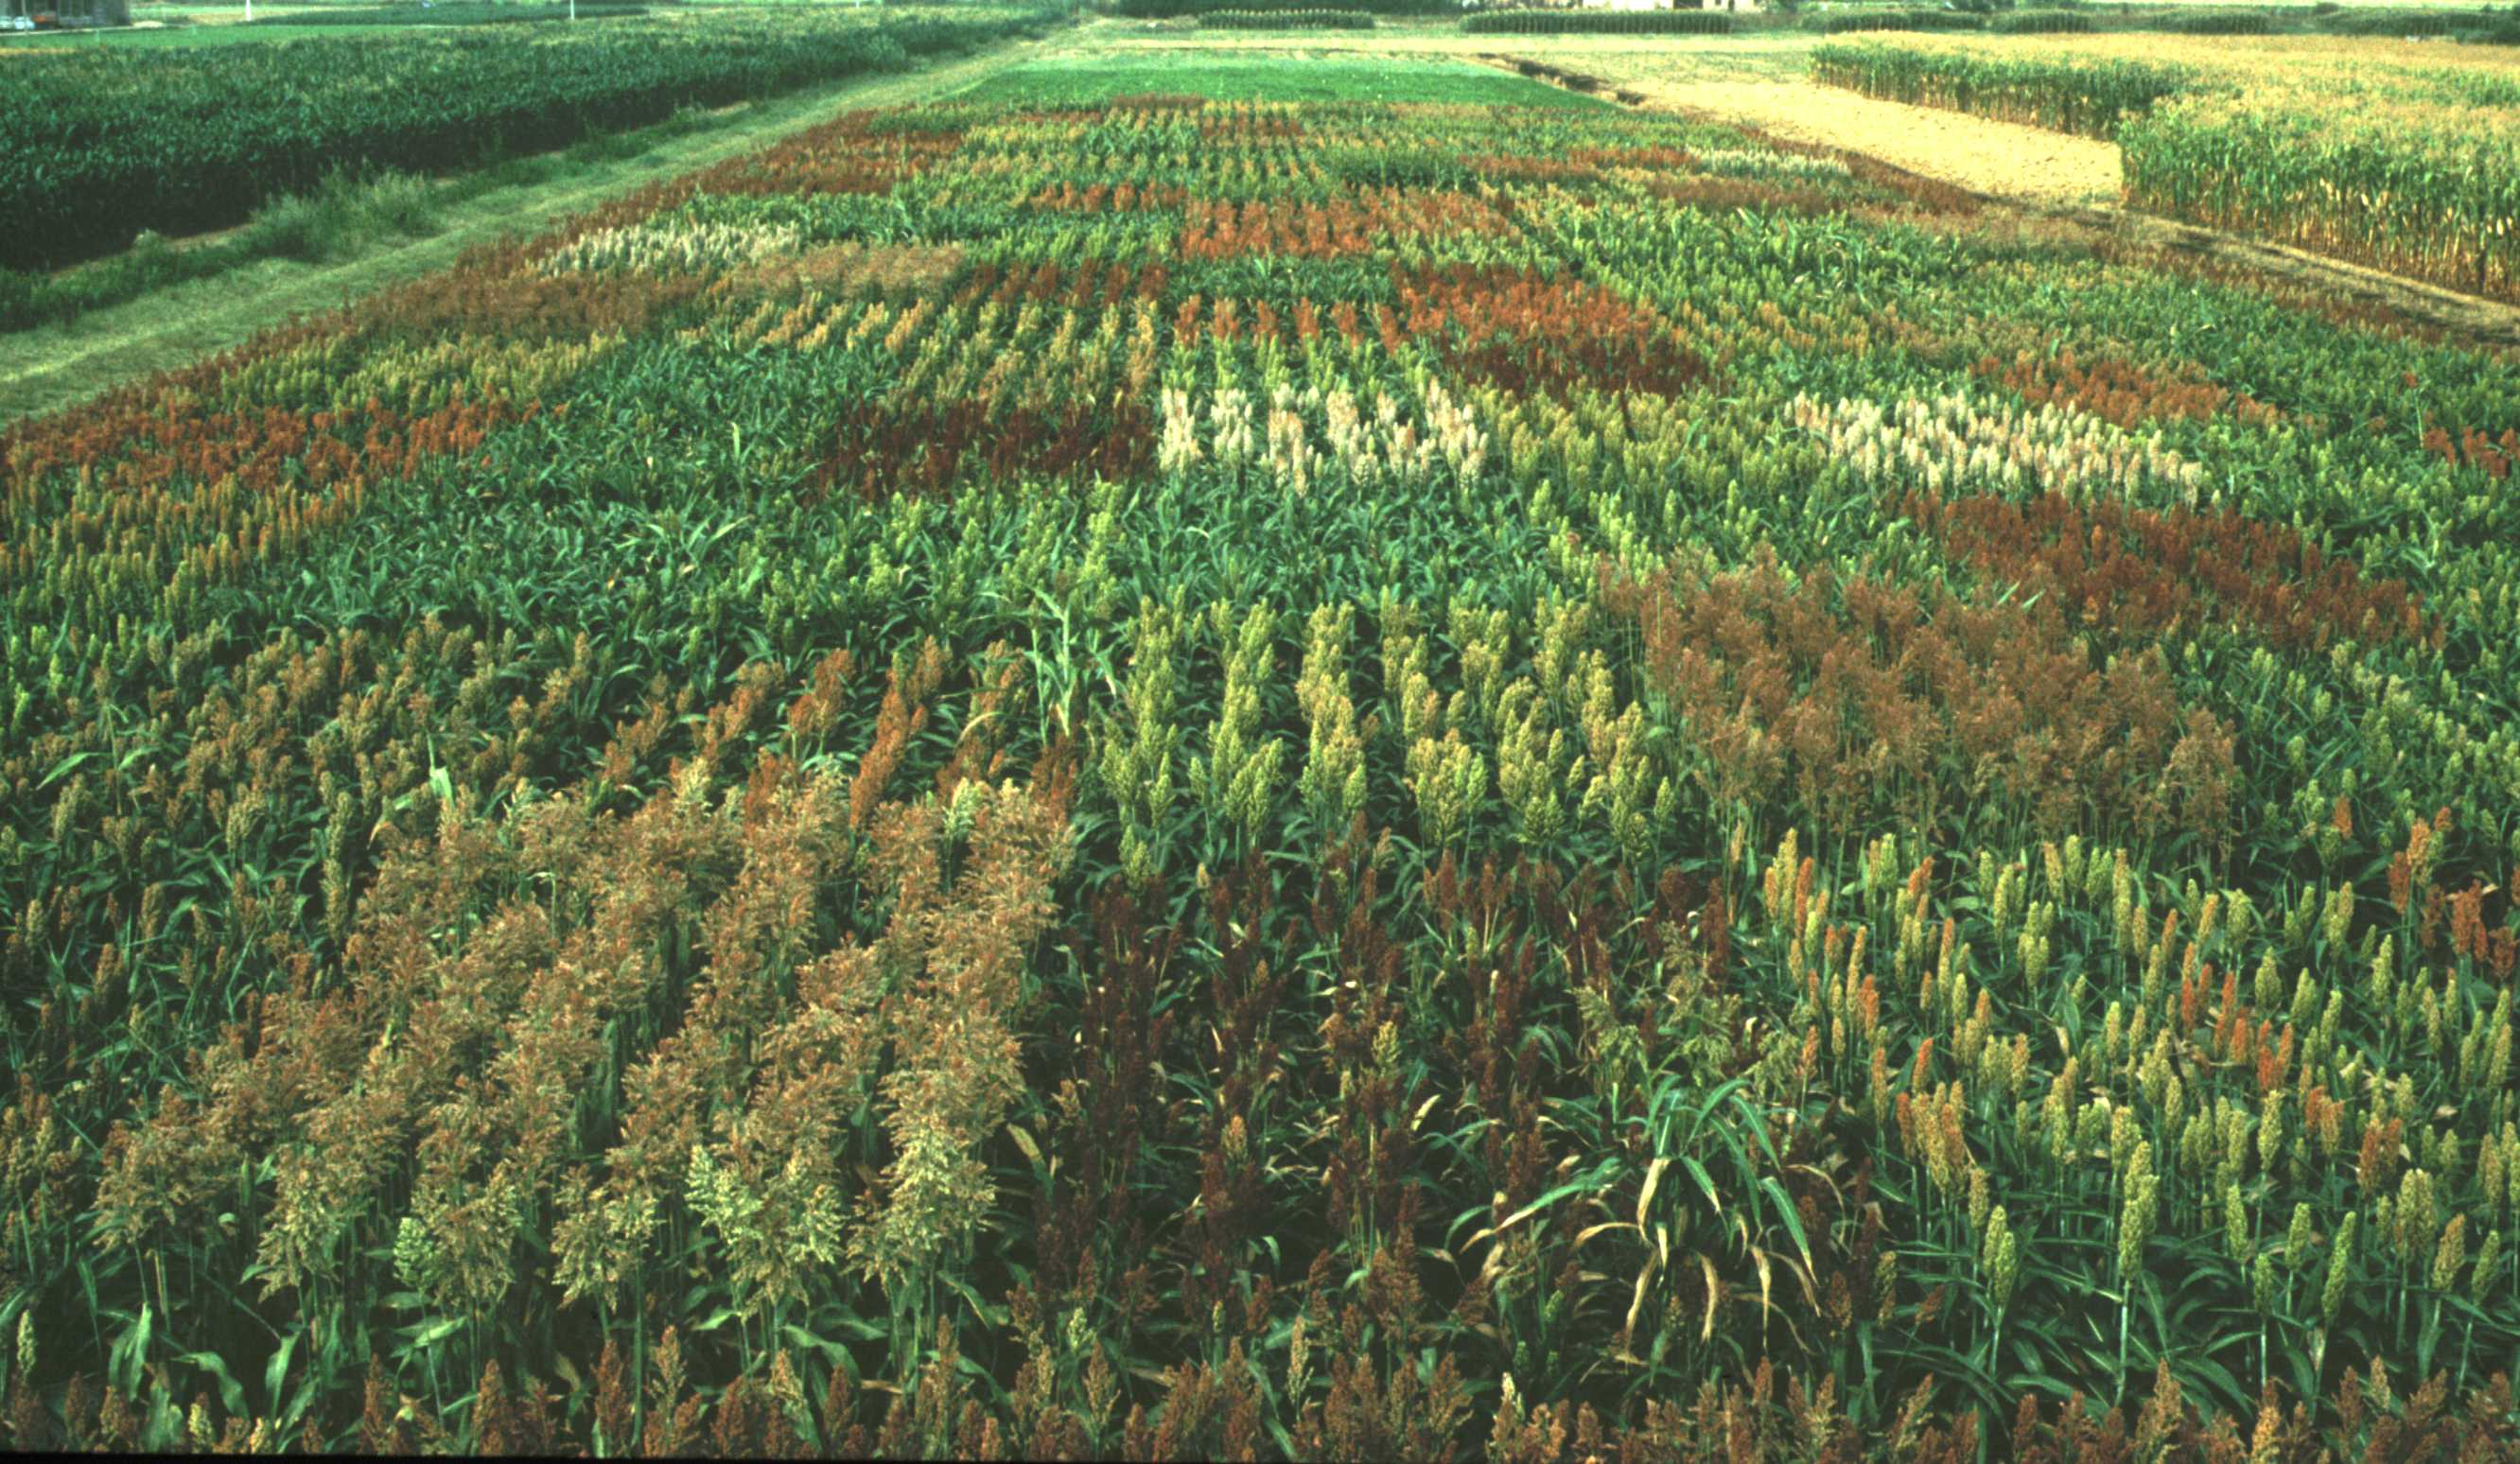
\includegraphics[width=0.9\linewidth]{_images/SorgoProveVarietali} 

}

\caption{Una prova sperimentale in campo (Foto D. Alberati)}\label{fig:figName21}
\end{figure}

Le parcelle vengono identificate dopo aver selezionato l'appezzamento giusto e averlo reso più uniforme possibile. Questa identificazione viene usualmente eseguita su carta, redigendo la \textbf{mappa dell'esperimento}.

In primo luogo, si decide la \textbf{dimensione e la forma della parcella}. L'aspetto fondamentale è che ogni parcella deve contenere un numero di piante sufficientemente alto da essere rappresentativo. Per questo motivo le colture a bassa fittezza (es. mais) hanno sempre bisogno di parcelle più grandi che non quelle ad alta fittezza (es. frumento). La dimensione non deve tuttavia eccedere una certa soglia, in quanto con essa aumenta anche la variabilità del terreno e, di conseguenza, diminuisce l'omogeneità dell'esperimento. Per questo motivo, talvolta si preferisce diminuire la dimensione delle parcelle ed, avendo lo spazio sufficiente, aumentare il numero delle repliche.

Nello stabilire la dimensione delle parcelle, dovremo tener conto del fatto che la parte più delicata è il bordo, in quanto le piante che si trovano lungo il bordo esterno risentono di condizioni diverse dalle altre piante situate al centro della parcella (\textbf{effetto bordo}). Questo determina variabilità all'interno della parcella, che possiamo minimizzare raccogliendo solo la parte centrale. Si viene così a distinguere la superficie totale della parcella dalla superficie di raccolta (\textbf{superficie utile}), che può essere anche molto minore di quella totale.

Tenendo conto degli aspetti detti in precedenza, ritieniamo che le colture ad elevata fittezza (frumento, cereali, erba medica\ldots{}) dovrebbero avere parcelle di almeno 10-20 m\textsuperscript{2}, mentre a bassa fittezza (mais, girasole\ldots{}) dovrebbero avere parcelle di almeno 20-40 m\textsuperscript{2}. Queste dimensioni sono riferite alla superficie utile di raccolta, non alla dimensione totale: se si ritiene di dover raccogliere solo una parte della parcella per limitare l'effetto bordo, allora le dimensioni totali dovranno essere opportunamente aumentate, rispetto a quanto indicato sopra.

Per quanto riguarda la forma, le parcelle quadrate minimizzano l'effetto bordo, perché, a parità di superficie, hanno un perimetro più basso. Tuttavia esse sono di più difficile gestione, in quanto, considerando il fronte di lavoro di una seminatrice o una mietitrebbiatrice parcellare, possono richiedere la semina o la raccolta in più passate, il che finisce per essere una fonte di errore. Per questo motivo le parcelle sono usualmente rettangolari, con una larghezza pari a quella della macchina impiegata per la semina.

Dopo aver stabilito la forma e la dimensione delle parcelle, si può procedere alla redazione della mappa, tenendo conto che il numero delle parcelle risulta dal prodotto tra il numero delle tesi sperimentali e il numero delle repliche.

In genere, si cerca di fare in modo che l'esperimento no sia troppo lungo (il che potrebbe aumenterebbe la variabilità), ma neanche troppo largo, per evitare di avvicinarsi troppo alle scoline, dove possono manifestarsi ristagni idrici. Lungo il contorno della prova è possibile sistemare altre parcelle fuori esperimento con funzione di `bordi'. In questo modo si evita che i bordi esterni delle parcelle esterne siano esposti a condizioni molto diverse dagli altri, cosa che potrebbe accentuare l'effetto `bordo', di cui abbiamo parlato in precedenza. Queste parcelle di bordo verranno trattate in modo ordinario (semina e diserbo tradizionale del pomodoro).

La figura \ref{fig:figName31} riporta la mappa di un esperimento sistemato su un appezzamento largo 30 metri e lungo 400 metri. In questo caso abbiamo disegnato otto file di parcelle in senso trasversale (8 x 2.25 m = 18 m di larghezza), e quattro parcelle in senso longitudinale. Vediamo in figura che la mappa riporta tutte le informazioni relative al disegno sperimentale, inclusa del Nord, in modo da facilitare l'orientamento della mappa stessa. Un altro fondamentale aspetto è che le parcelle sono tutte chiaramente identificate con un numero.

\begin{figure}

{\centering 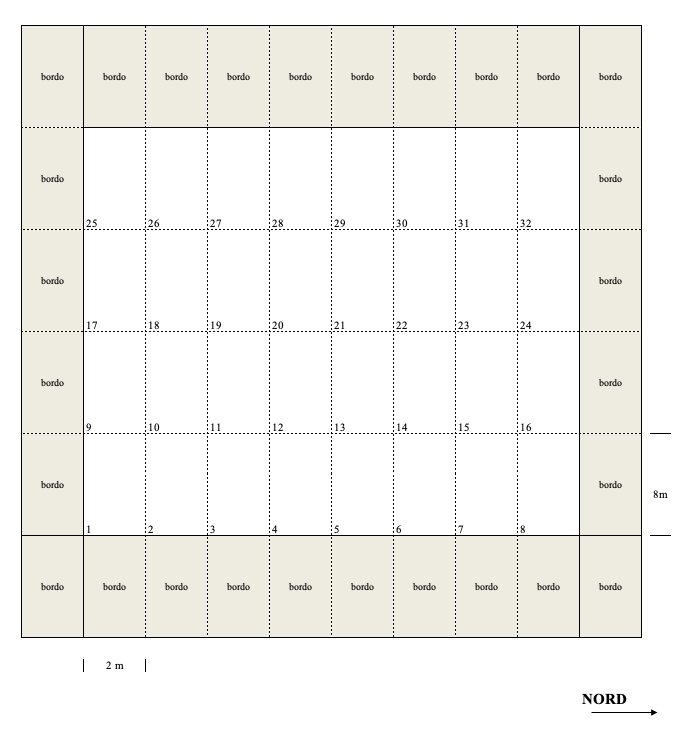
\includegraphics[width=0.9\linewidth]{_images/Mappa1} 

}

\caption{Mappa di campo di un esperimento con 32 parcelle}\label{fig:figName31}
\end{figure}

\hypertarget{e-se-ricercatorisoggetti-sono-influenzabili}{%
\subsubsection{E se ricercatori/soggetti sono influenzabili?}\label{e-se-ricercatorisoggetti-sono-influenzabili}}

Per concludere questa parte, è opportuno menzionare il fatto che, in un esperimento scientifico, il fatto che lo sperimentatore e il soggetto siano coscienti del trattamento somministrato può portare a risultati distorti. Per esempio, nell'eseguire un rilievo, lo sperimentatore può essere influenzato dal sapere con quale diserbante è stata trattata una parcella, cercando inconsciamente conferme alle sue conoscenze pregresse. D'altro canto, nei soggetti sperimentali dotati di coscienza (uomo) sapere di essere stati trattati può influenzare l'esito del trattamento (effetto placebo).

Per evitare questi problemi, soprattutto in ambito medico, un esperimento può essere pianificato come:

\begin{enumerate}
\def\labelenumi{\arabic{enumi}.}
\tightlist
\item
  cieco: l'unità sperimentale o lo sperimentatore non sono coscienti dei dettagli del trattamento;
\item
  doppio cieco: né l'unità sperimentale né lo sperimentatore sono a coscienza dei dettagli del trattamento
\end{enumerate}

Un esperimento cieco e/o doppio cieco possono non essere eticamente corretti oppure inutili, nel qual caso si torna ad un esperimento tradizionale `aperto' (\emph{open experiment}: Tutti sanno tutto')

\hypertarget{allocazione-dei-trattamenti-e-disegno-sperimentale}{%
\section{Allocazione dei trattamenti e disegno sperimentale}\label{allocazione-dei-trattamenti-e-disegno-sperimentale}}

Il problema dell'allocazione dei trattamenti non si pone con gli esperimenti osservazionali, in quanto con questi si scelgono unità sperimentali già `naturalmente' trattate.

Per tutti gli esperimenti disegnati si pone invece il problema di scegliere quali soggetti trattare e con cosa. A seconda di quali vincoli introduciamo nella selezioni dei soggetti possiamo avere diversi schemi sperimentali. Quelli che descriviamo di seguito, sono quelli più comunemente usati nella sperimentazione di pieno campo, ma, con le opportune modifiche, possono trovare impiego anche in molte altre discipline scientifiche.

\hypertarget{disegni-completamente-randomizzati}{%
\subsection{Disegni completamente randomizzati}\label{disegni-completamente-randomizzati}}

Per queste prove, le più semplici, la scelta dei soggetti da trattare è totalmente casuale, senza vincoli di sorta. Il vantaggio principale è la semplicità; lo svantaggio sta nel fatto che tutte le eventuali differenze e disomogeneità tra unità sperimentali restano non riconosciute ed entrano nella definizione dell'errore sperimentale. Per questo, i disegno completamente randomizzati sono utilizzato soprattutto per le situazioni di buona uniformità ambientale e tra i soggetti.

Come esempio mostriamo un disegno completamente randomizzato utilizzando le parcelle della figura \ref{fig:figName31}, dove abbiamo allocato 8 trattamenti) identificati con le lettere da A ad H) con quattro repliche. Come si può notare, l'allocazione è completamente casuale (figura \ref{fig:figName33})

\begin{figure}

{\centering 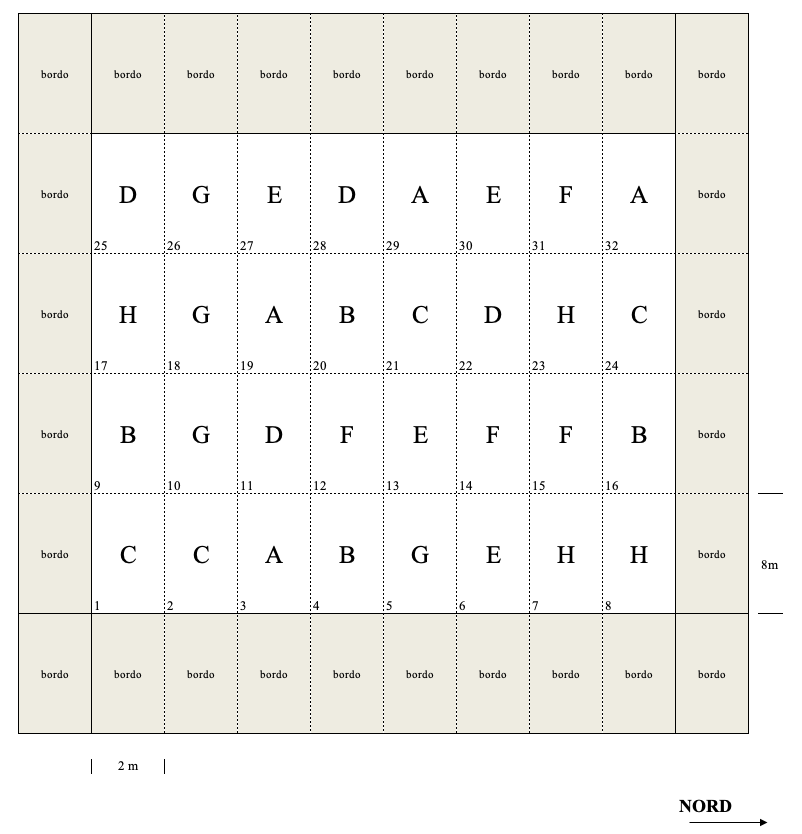
\includegraphics[width=0.9\linewidth]{_images/Mappa1CRD} 

}

\caption{Esempio di uno schema sperimentale a randomizzazione completa}\label{fig:figName33}
\end{figure}

\hypertarget{disegni-a-blocchi-randomizzati}{%
\subsection{Disegni a blocchi randomizzati}\label{disegni-a-blocchi-randomizzati}}

Le unità sperimentali non sono sempre omogenee, ma possono presentare delle differenze, ad esempio di fertilità, oppure di sesso. In queste condizioni, la randomizzione completa potrebbe favorire situazioni di `confounding'; ad esempio, potrebbe capitare che un trattamento venga allocato alle parcelle più fertili e quindi che sia avvantaggiato rispetto ad un altro. In queste condizioni, può essere utile dividere i soggetti in più gruppi omogenei, tenendo conto di:

\begin{enumerate}
\def\labelenumi{\arabic{enumi}.}
\tightlist
\item
  vicinanza spaziale (campi, parcelle, stalle \ldots{})
\item
  caratteristiche fisiche (età, peso, sesso \ldots{} )
\item
  vicinanza temporale
\item
  gestione dei compiti (tecnico, valutatore, giudice \ldots{})
\end{enumerate}

Successivamente, i trattamenti vengono allocati in modo randomizzato all'interno di ogni gruppo, in modo che ognuno di essi abbi una sola replica per gruppo e sia presente in tutti i gruppi. I disegni di questo tipo si dicono a blocchi randomizzati.

Ad esempio, nel caso dello schema in figura \ref{fig:figName31}, è lecito aspettarsi un gradiente trasversale, dato che il campo sarà certamente meno fertile vicino alle scoline. Per questo motivo, dato che abbiamo scelto di fare quattro repliche, divideremo l'appezzamento in quattro blocchi perpendicolari al gradiente di fertilità. Ad esempio il blocco 1 conterrà le parcelle 1, 9, 17, 25, 2, 10, 18 e 26, cioè le prime due colonne della mappa, con un numero di parcelle esattamente uguali al numero delle tesi. Il blocco 2 conterrà le colonne 3 e 4 e così via. Dato che il gradiente è trasversale, le parcelle di un stesso blocco saranno più omogenee che non parcelle su blocchi diversi. Dopo aver diviso la mappa in quattro blocchi di otto parcelle, possiamo allocare gli otto trattamenti a random all'interno di ogni blocco (\ref{fig:figName34})

\begin{figure}

{\centering 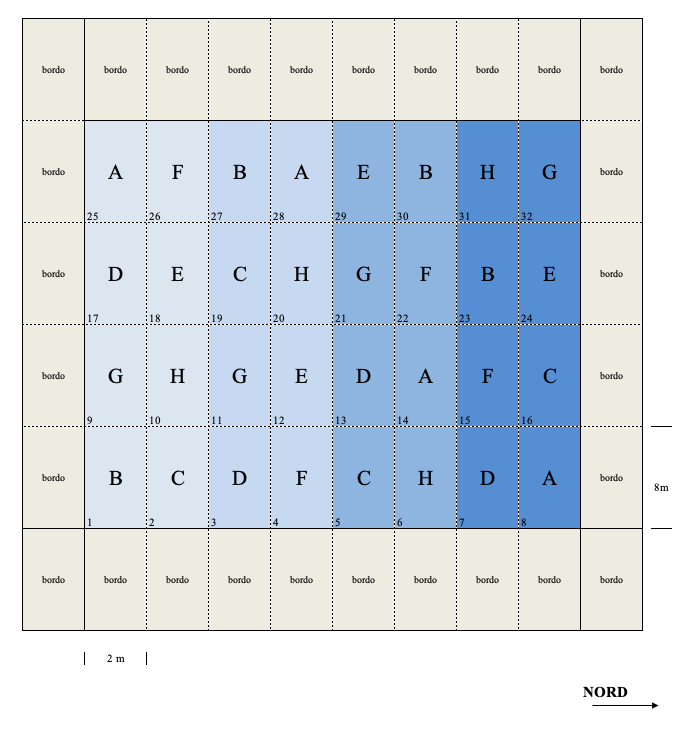
\includegraphics[width=0.9\linewidth]{_images/Mappa1CRBD} 

}

\caption{Esempio di uno schema sperimentale a blocchi randomizzati}\label{fig:figName34}
\end{figure}

Un disegno a blocchi randomizzati non è solo tipico della sperimentazione di campo. Ad esempio, volendo determinare la contaminazione da micotossine nelle confezioni di datteri, a seconda della modalità di confezionamento (es. carta, busta di plastica, scatola di plastica perforata), si può sospettare che il supermercato nel quale le confezioni vengono vendute potrebbe avere un certo effetto, legato alle modalità di conservazione. Per cui, invece che prelevare trenta confezioni (dieci per metodo) a caso nei supermercati di Perugia, scegliamo dieci supermercati e in ognuno, prendiamo una confezione per tipo. In questo caso, il supermercato fa da blocco.

In generale, potremmo immaginare un esperimento con trattamenti che vengono allocati a caso agli animali di una stalla e ripetuti su stalle diverse, o a soggetti in gruppi omogenei di età e così via.

Il vantaggio del disegno a blocchi randomizzati sta nel fatto che le differenze tra gruppi sono spiegabili attraverso l'appartenenza ad un determinato gruppo e possono quindi essere scorporate dal calcolo dell'errore sperimentale.

\hypertarget{disegni-a-quadrato-latino}{%
\subsection{Disegni a quadrato latino}\label{disegni-a-quadrato-latino}}

In questo caso, le unità sperimentali presentano due `gradienti', cioè vi sono differenze legate a due elementi importanti, oltre al trattamento sperimentale. Vediamo un esempio.

Una certo oggetto richiede un solo operatore per essere costruito, ma l'operazione può essere eseguita in quattro modi diversi. Vogliamo capire qual è il modo più veloce e, pertanto, pianifichiamo un esperimento. L'unità sperimentale è il lavoratore. I metodi sono quattro e, volendo lavorare con quattro repliche, avremmo bisogno di sedici operatori per disegnare un esperimento completamente randomizzato. Possiamo tuttavia considerare che un operatore, in quattro turni successivi, può operare con tutti e quattro i metodi. Quindi possiamo disegnare un esperimento in cui il turno fa da unità sperimentale e l'operatore fa da blocco (esperimento a blocchi randomizzati).

Tuttavia, in ogni blocco (operatore) vi è un gradiente, nel senso che i turni successivi al primo sono via via meno efficienti, perché l'operatore accumula stanchezza. Per tener conto di questo potremmo lasciare all'operatore un congruo periodo di tempo tra un turno e l'altro. Oppure, potremmo introdurre un vincolo ulteriore, per ogni operatore, randomizzando i quattro metodi tra i turni, in modo che ogni metodo, in operatori diversi, capiti in tutti i turni. In sostanza, l'operatore fa da blocco, perché in esso sono contenuti tutti i metodi. Ma anche il turno (per tutti gli operatori) fa da blocco, in quanto in esso sono ancora contenuti tutti i metodi. Proviamo a schematizzare, nella figura seguente (\ref{fig:figName391} ).

\begin{figure}

{\centering 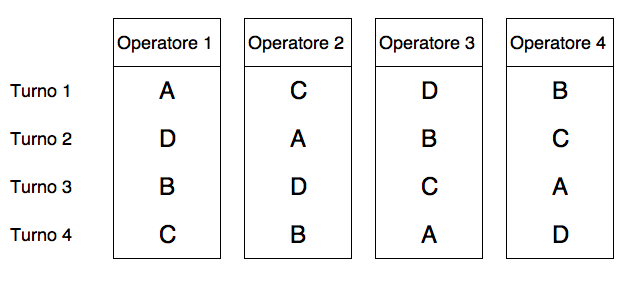
\includegraphics[width=0.9\linewidth]{_images/TurniOperatori} 

}

\caption{Allocazione di quattro metodi di lavoro (A, B, C e D), tra quattro operatori, in quattro turni, seguendo uno schema a quadrato latino}\label{fig:figName391}
\end{figure}

Questo schema prende il nome di quadrato latino, in quanto il numero delle repliche è uguale al numero dei trattamenti e, schematizzando lo schema su una mappa, otteniamo una griglia quadrata, nella quale ogni trattamento occupa tutte le righe e tutte le colonne. Chi lo conosce, riconosce in questo schema i principi di fondo del Sudoku.

Questo disegno è utile, perché possiamo dar conto sia delle differenza tra righe (turni), che delle differenze tra colonne (operatori), in modo da ridurre al minimo possibile la variabilità inspiegata. Lo svantaggio sta nel fatto che, dovendo avere tante repliche quanti sono i trattamenti, è utilizzabile solo per esperimenti abbastanza piccoli.

\hypertarget{blocking-ed-analisi-dei-dati}{%
\subsection{Blocking ed analisi dei dati}\label{blocking-ed-analisi-dei-dati}}

Sia i disegni a blocchi randomizzati che quelli a quadrato latino impongono vincoli alla randomizzazione, che, ricordiamo, è uno degli elementi fondamentali degli esperimenti scientifici. Posto che non si deve violare l'indipendenza delle repliche, l'inclusione di vincoli alla randomizzazione è consentita, \textbf{ma questa deve sempre essere tenuta presente in fase di analisi dei dati}.

Ronald Fisher diceva ``\emph{Analyse them as you have randomised them}''. Meglio seguire il consiglio.

\hypertarget{scelta-delle-variabili-da-rilevare}{%
\section{Scelta delle variabili da rilevare}\label{scelta-delle-variabili-da-rilevare}}

Durate e al termine dell'esperimento, sarà necessario rilevare le più importanti caratteristiche dei soggetti sperimentali, sia quelle innate, sia quelle indotte dai trattamenti sperimentali. Per ogni singolo carattere, l'insieme delle modalità/valori che ognuno dei soggetti presenta prende il nome di \textbf{variabile} (proprio perché varia, cioè assume diversi valori, a seconda del soggetto). Ad esempio, quando stiamo studiando l'effetto di due diserbanti su piante infestanti appartenenti ad una certa specie, posto che l'unità sperimentale è costituita da una singola pianta, possiamo avere le seguenti variabili: il prodotto diserbante con cui ogni pianta è stata trattata, il peso di ogni pianta prima del trattamento, il peso di ogni pianta dopo il trattamento.

Le variabili sperimentali possono essere molto diverse tra di loro ed è piuttosto importante saperle riconoscere, perché questo condiziona il tipo di analisi statistica da eseguire.

\hypertarget{variabili-nominali-categoriche}{%
\subsection{Variabili nominali (categoriche)}\label{variabili-nominali-categoriche}}

Le variabili nominali esprimono, per ciascun soggetto, l'appartenenza ad una determinata categoria o raggruppamento. L'unica caratteristica delle categorie è l'esclusività, cioè un soggetto che appartiene ad una di esse non può appartenere a nessuna delle altre. Variabili nominali sono, ad esempio, il sesso, la varietà, il tipo di diserbante impiegato, la modalità di lavorazione e così via. Le variabili categoriche permettono di raggruppare i soggetti, ma non possono essere utilizzate per fare calcoli, se non per definire le proporzioni dei soggetti in ciascun gruppo.

\hypertarget{variabili-ordinali}{%
\subsection{Variabili ordinali}\label{variabili-ordinali}}

Anche le variabili ordinali esprimono, per ciascun soggetto, l'appartenenza ad una determinata categoria o raggruppamento. Tuttavia, le diverse categorie sono caratterizzate, oltre che dall'esclusività, anche da una relazione di ordine, nel senso che è possibile stabilire una naturale graduatoria tra esse. Ad esempio, la risposta degli agricoltori a domande relative alla loro percezione sull'utilità di una pratica agronomica può essere espressa utilizzando una scala con sei categorie (0, 1, 2, 3, 4 e 5), in ordine crescente da 0 a 5 (scala Likert). Di conseguenza possiamo confrontare categorie diverse ed esprimere un giudizio di ordine (2 è maggiore di 1, 3 è minore di 5), ma non possiamo eseguire operazioni matematiche, tipo sottrarre dalla categoria 3 la categoria 2 e così via, dato che la distanza tra le categorie non è necessariamente la stessa.

\hypertarget{variabili-quantitative-discrete}{%
\subsection{Variabili quantitative discrete}\label{variabili-quantitative-discrete}}

Le variabili discrete sono caratterizzate dal fatto che possiedono, oltre alle proprietà dell'esclusività e dell'ordine, anche quella dell'equidistanza tra gli attributi (es., in una scala a 5 punti, la distanza -- o la differenza -- fra 1 e 3 è uguale a quella fra 2 e 4 e doppia di quella tra 1 e 2). Una tipica variabile discreta è il conteggio di piante infestanti all'interno di una parcella di terreno.

Le variabili discrete consentono la gran parte delle operazioni matematiche e permettono di calcolare molte importanti statistiche come la media, la mediana, la varianza e la deviazione standard.

\hypertarget{variabili-quantitative-continue}{%
\subsection{Variabili quantitative continue}\label{variabili-quantitative-continue}}

Le variabili quantitative continue possiedono tutte le proprietà precedentemente esposte (esclusività delle categorie, ordine, distanza) oltre alla continuità, almeno in un certo intervallo. Tipiche variabili continue sono l'altezza, la produzione, il tempo, la fittezza\ldots{}

Dato che gli strumenti di misura nella realtà sono caratterizzati da una certa risoluzione, si potrebbe arguire che misure su scala continua effettivamente non esistono. Tuttavia questo argomento è più teorico che pratico e, nella ricerca biologica, consideriamo continue tutte le misure nelle quali la risoluzione dello strumento è sufficientemente piccola rispetto alla grandezza da misurare. Viceversa, le variabili continue sono piuttosto rare nelle scienze economiche e sociali in genere.

La quantità di informazione fornita dagli strumenti di valutazione cresce passando dalle scale nominali, di più basso livello, a quelle quantitative continue, di livello più elevato. Variabili esprimibili con scale quantitative continue o discrete possono essere espresse anche con scale qualitative, adottando un'opportuna operazione di classamento. Il contrario, cioè trasformare in quantitativa una variabile qualitativa, non è invece possibile.

\hypertarget{rilievi-visivi-e-sensoriali}{%
\subsection{Rilievi visivi e sensoriali}\label{rilievi-visivi-e-sensoriali}}

Nella pratica sperimentale è molto frequente l'adozione di metodi di rilievo basati sull'osservazione di un fenomeno attraverso uno dei sensi (più spesso, la vista, ma anche gusto e olfatto) e l'assegnazione di una valutazione su scala categorica, ordinale o, con un po' di prudenza, quantitativa discreta o continua. Ad esempio, il ricoprimento delle piante infestanti, la percentuale di controllo di un erbicida e la sua fitotossicità vengono spesso rilevati visivamente, su scale da 0 a 100 o simili.

I vantaggi di questa tecnica sono molteplici:

\begin{enumerate}
\def\labelenumi{\arabic{enumi}.}
\tightlist
\item
  Basso costo ed elevata velocità
\item
  Possibilità di tener conto di alcuni fattori perturbativi esterni, che sono esclusi dalla valutazione, contrariamente a quello che succede con metodi oggettivi di misura
\item
  non richiede strumentazione costosa
\end{enumerate}

A questi vantaggi fanno da contraltare alcuni svantaggi, cioè:

\begin{enumerate}
\def\labelenumi{\arabic{enumi}.}
\tightlist
\item
  Minor precisione (in generale)
\item
  Soggettività
\item
  L'osservatore può essere prevenuto
\item
  Difficoltà di mantenere uniformità di giudizio
\item
  Richiede esperienza specifica e allenamento
\end{enumerate}

I rilievi sensoriali sono ben accettati nella pratica scientifica in alcuni ambiti ben definiti, anche se richiedono attenzione nell'analisi dei dati non potendo essere assimilati \emph{tout court} con le misure oggettive su scala continua.

\hypertarget{variabili-di-confondimento}{%
\subsection{Variabili di confondimento}\label{variabili-di-confondimento}}

Quando si pianificano i rilievi da eseguire, oppure anche nel corso dell'esecuzione di un esperimento, bisogna tener presente non soltanto la variabile che esprime l'effetto del trattamento, ma anche tutte le variabili che misurano possibili fattori di confondimento.

Ad esempio, immaginiamo di voler valutare la produttività di una specie arborea in funzione della varietà. Immaginiamo anche di sapere che, per questa specie, la produttività dipende anche dall'età. Se facciamo un esperimento possiamo utilizzare alberi della stessa età per minimizzare la variabilità dei soggetti. Tuttavia, se questo non fosse possibile, per ogni albero dobbiamo rilevare non solo la produttività, ma anche l'età, in modo da poter valutare anche l'effetto di questo fattore aggiuntivo e separarlo dall'effetto della varietà. In questo modo l'esperimento diviene molto più preciso.

\hypertarget{impianto-delle-prove}{%
\section{Impianto delle prove}\label{impianto-delle-prove}}

Da questo punto in poi, subentrano le competenze agronomiche e fitopatologiche necessarie per condurre gli esperimenti, Mi piace solo ricordare alcune pratiche usuali nella sperimentazione di pieno campo, destinate a migliorare l'efficienza della prova.

\begin{enumerate}
\def\labelenumi{\arabic{enumi}.}
\tightlist
\item
  Seminare a densità più alte e poi diradare, per assicurare una migliore uniformità di impianto
\item
  Prelevare da ogni parcella più campioni ed, eventualmente, omogeneizzarli o mediare i risultati ottenuti (vedi il caso dei 1000 semi)
\item
  Considerare le caratteristiche naturalmente meno variabili (es. la produzione areica e non la produzione per pianta)
\end{enumerate}

Voglio inoltre ricordare che gli esperimenti parcellari configurano una situazione nella quale, per l'elevata cura che si pone nelle tecniche agronomiche, si riesce ad ottenere una produttività almeno del 20\% superiore rispetto a quanto avviene nella normale pratica agricola.

\hypertarget{scrivere-un-progettoreport-di-ricerca-semplici-indicazioni}{%
\section{Scrivere un progetto/report di ricerca: semplici indicazioni}\label{scrivere-un-progettoreport-di-ricerca-semplici-indicazioni}}

Quanto abbiamo finora esposto costituisce uno schema generale che può essere adottato per redigere un progetto di ricerca o un report sui risultati ottenuti (tesi, pubblicazione). Bisogna provare che la ricerca che si è eseguita è precisa, accurata e replicabile/riproducibile e, di conseguenza, i risultati sono validi.

Nella redazione di un progetto di ricerca o di un report, è fondamentale tratteggiare bene i seguenti elementi:

\begin{enumerate}
\def\labelenumi{\arabic{enumi}.}
\tightlist
\item
  Titolo della ricerca
\item
  Descrizione del problema e background scientifico
\item
  Ipotesi scientifica, motivazioni e obiettivi
\item
  Tipo di esperimento e durata
\item
  Disegno sperimentale: trattamenti sperimentali (tesi) a confronto con dettagli relativi all'applicazione
\item
  Unità sperimentali e criteri per la loro selezione. Dettagli su repliche e randomizzazione
\item
  Dettagli su eventuali tecniche di `blocking'
\item
  Variabili da rilevare/rilevate
\item
  Dettagli su come le variabili saranno/sono state rilevate
\item
  Esposizione dei risultati (solo report)
\item
  Discussione (solo report)
\item
  Conclusioni (solo report)
\end{enumerate}

Alcuni aspetti che divengono elemento di valutazione del progetto e/o del report sono i seguenti:

\begin{enumerate}
\def\labelenumi{\arabic{enumi}.}
\tightlist
\item
  La selezione dei metodi deve essere coerente con gli obiettivi
\item
  Descrizione dettagliata dei materiali e metodi (bisogna che chiunque sia in grado di replicare l'esperimento)
\item
  Esposizione dei risultati chiara e convincente
\item
  Discussione approfondita e con molti riferimenti alla letteratura.
\end{enumerate}

\begin{center}\rule{0.5\linewidth}{\linethickness}\end{center}

\hypertarget{per-approfondire-un-po-1}{%
\section{Per approfondire un po'\ldots{}}\label{per-approfondire-un-po-1}}

\begin{enumerate}
\def\labelenumi{\arabic{enumi}.}
\tightlist
\item
  Cochran, W.G., Cox, G.M., 1950. Experimental design. John Wiley \& Sons, Inc., Books.
\item
  Daniel, J., 2011. Sampling Essentials: Practical Guidelines for Making Sampling Choices. USA: SAGE.
\item
  LeClerg, E.L., Leonard, W.H., Clark, A.G., 1962. Field Plot Technique. Burgess Publishing Company, Books.
\end{enumerate}

\hypertarget{modelli-matematici-ed-analisi-dei-dati}{%
\chapter{Modelli matematici ed analisi dei dati}\label{modelli-matematici-ed-analisi-dei-dati}}

L'eredità galileiana ci porta ad immaginare che il funzionamento della natura sia basato su una serie di relazioni causa-effetto, descrivibili utilizzando il linguaggio universale della matematica. La conoscenza esatta di queste relazioni, nella teoria, ci potrebbe consentire di prevedere l'andamento di ogni fenomeno naturale, almeno quelli osservabili con sufficiente precisione.

In effetti era proprio questa l'ambizione più grande degli scienziati all'inizio dell'ottocento: conoscendo lo stato iniziale di un sistema, doveva essere possibile prevederne l'evoluzione futura. In realtà si è ben presto scoperto che si trattava di un'ambizione irrealistica, non tanto e non solo per la comparsa della meccanica quantistica un secolo dopo, ma anche per l'aumento di importanza degli studi in ambito psichiatrico e medico/biologico. Questi studi, infatti, venivano (e vengono) eseguiti su organismi viventi molto complessi, che, se sottoposti allo stesso stimolo, danno risposte altamente variabili e, spesso, anche difficilmente misurabili e controllabili. Immaginiamo quanto possa essere difficile quantificare uno stato legato ad una patologia mentale e individuare un pattern di risposta ad un certo stimolo, ad esempio farmacologico.

Queste difficoltà fecero prevalere, tra i biologi, la convinzione che la natura funzionasse in base a meccanismi deterministici ben definiti, anche se difficilmente osservabili nella pratica sperimentale, a causa dei numerosi elementi d'incertezza che si manifestavano nel corso delle osservazioni sperimentali. Insomma, la natura è perfetta, ma l'osservazione è fallace, perché influenzata dalla presenza di una forte componente stocastica e imprevedibile, che va sotto il nome generico di 'errore sperimentale'.

Dell'errore sperimentale abbiamo già parlato nei capitoli precedenti. Abbiamo anche visto che Ronald Fisher, nel suo famoso testo ``Il disegno degli esperimenti'' ha posto le basi per una corretta metodica sperimentale, volta a minimizzare l'impatto della componente stocastica e, soprattutto, ad impedire che essa possa confondersi con gli effetti degli stimoli sperimentali in studio. Minimizzare, tuttavia, non significa eliminare ed è evidente che, pur con tutti gli sforzi possibili, i risultati sperimentali saranno influenzati sempre e comunque da una certa quota di variabilità stocastica. Si vengono quindi a creare due contrapposte situazioni:

\begin{enumerate}
\def\labelenumi{\arabic{enumi}.}
\tightlist
\item
  la verità `vera', immanente, che `agisce' in base a meccanismi deterministici causa-effetto ben definiti.
\item
  La `verità' sperimentale, che si produce a partire dalla verità `vera', per effetto dell'azione di elementi perturbativi casuali, che non ci permettono di osservare la verità `vera'.
\end{enumerate}

Tenendo conto di questo, nella logica galileiana, possiamo provare ad utilizzare dei modelli matematici per descrivere le nostre osservazioni sperimentali e come esse si producono. Tuttavia, nessun modello è da considerare completo, se non è caratterizzato dalla capacità di descrivere sia la componente deterministica che quella stocastica, che sono alla base della formazione delle osservazioni sperimentali.

\hypertarget{verita-vera-e-modelli-deterministici}{%
\section{Verità `vera' e modelli deterministici}\label{verita-vera-e-modelli-deterministici}}

In semplice linguaggio algebrico, possiamo porre un modello deterministico causa-effetto utilizzando una funzione di questo tipo:

\[ Y_E = f(X, \theta) \]

dove \(Y_E\) è l'effetto atteso dello stimolo \(X\), secondo la funzione \(f\), basata su una collezioni di parametri \(\theta\).

In questo modello vi sono una serie di componenti, che proviamo a guardare un po' più nel dettaglio.

La risposta attesa (\(Y_E\)) è l'oggetto del nostro studio e può assumere le forme più disparate: spesso è numerica, ma a volte rappresenta una qualità. In questo libro consideremo solo la situazione in cui \(Y\) è rappresentato da una sola variabile (analisi univariata), ma esistono casi in cui viene osservata e analizzata la risposta di soggetti in relazione a molte variabili (analisi multivariata).

Lo stimolo sperimentale (\(X\)) è costituito da una o più variabili continue, discrete o categoriche, che rappresenta/ano il/i trattamento/i sperimentale/i (fattore/i sperimentale/i). Insieme ad \(Y\), è l'elemento noto di un esperimento, in quanto viene definito \emph{a priori} con il disegno sperimentale.

La `funzione' di risposta (\(f\)) è un'equazione, altrimenti detta `modello matematico'. L'equazione può essere lineare o non-lineare ed è selezionata o in base a considerazioni di carattere biologico, o con un approccio puramente empirico, nel quale osservo la risposta e scelgo un'equazione la cui forma si adatta bene ad essa.

I parametri di una funzione (\(\theta\)) sono un insieme di valori numerici che definiscono il modello. Nel prossimo paragrafo vedremo qualche esempio.

\hypertarget{qualche-esempio-di-modello-deterministico}{%
\subsection{Qualche esempio di modello deterministico}\label{qualche-esempio-di-modello-deterministico}}

Il modello più semplice è il cosiddetto modello della media:

\[ Y = \mu \]

Con questo modello si vuole indicare che un'osservazione dovrebbe conformarsi ad un certo valore atteso, come effetto di un unico stimolo sperimentale noto. Ha un solo parametro, cioè \(\mu\).

Un modello analogo, ma più complesso è il cosidetto modello ANOVA:

\[
Y = \left\{ {\begin{array}{ll}
\mu_1 & se \quad X = A \\
\mu_2 & se \quad X = B
\end{array}} \right.
\]

In questo caso la risposta attesa dipende dallo stimolo sperimentale X, che è composto di due trattamenti: se il soggetto è trattato con A, fornisce la risposta \(\mu_1\), se è trattato con B fornisce \(\mu_2\). Il trattamento sperimentale è costituito da una variabile categorica con due modalità, ma l'estensione a più modalità è immediata. In questo caso, abbiamo due parametri (\(\mu_1\) e \(\mu_2\)).

Un ulteriore esempio di modello che vedremo in questo libro è la regressione lineare semplice, dove la relazione di risposta è descrivibile con una retta, la cui equazione generale è:

\[ Y = a + b \times X \]

In questo caso sia la \(Y\) che la \(X\) sono variabili quantitative e vi sono due parametri \(a\) e \(b\).

I modelli finora descritti sono lineari, ma esistono numerosi funzioni che descrivono relazioni curvilinee. Come, ad esempio, la parabola:

\[ Y = a + b \, X + c \, X^2\]
caratterizzata da tre parametri, oppure la funzione esponenziale:

\[ Y = a \, e^{b X} \]

caratterizzata da due parametri (\(a\) e \(b\)), mentre \(e\) è l'operatore di Nepero. Delle funzioni curvilinea parleremo al termine di questo libro.

\hypertarget{genesi-deterministica-delle-osservazioni-sperimentali}{%
\section{Genesi deterministica delle osservazioni sperimentali}\label{genesi-deterministica-delle-osservazioni-sperimentali}}

Le equazioni esposte più sopra sono tutte nella loro forma generale e non sono utilizzabili se ai parametri non viene sostituito un valore numerico. E'proprio questo il nostro punto di partenza: un fenomeno scientifico può essere descritto attraverso un'equazione e dei parametri.

Ad esempio, potremmo immaginare che la risposta produttiva (Y) di una coltura (es. frumento) dipenda dalla dose della concimazione azotata (X), seguendo un andamento lineare, con \(a = 20\) e \(b = 0.3\). Rifacendosi alla notazione esposta sopra diremo che \(\theta\) è l'insieme dei valori 20 e 0.3.

Se questo assunto è vero, un eventuale esperimento di concimazione azotata, in assenza di qualunque fattore perturbativo, dovrebbe dare risultati assolutamento prevedili. Ad esempio, se concimiamo il frumento con 0, 30, 60, 90, 120 e 150 kg/ha di azoto, dovremmo osservare le risposte riportate qui di seguito.

\begin{Shaded}
\begin{Highlighting}[]
\NormalTok{X <-}\StringTok{ }\KeywordTok{c}\NormalTok{(}\DecValTok{0}\NormalTok{, }\DecValTok{30}\NormalTok{, }\DecValTok{60}\NormalTok{, }\DecValTok{90}\NormalTok{, }\DecValTok{120}\NormalTok{, }\DecValTok{150}\NormalTok{)}
\NormalTok{Ye <-}\StringTok{ }\DecValTok{20} \OperatorTok{+}\StringTok{ }\FloatTok{0.3} \OperatorTok{*}\StringTok{ }\NormalTok{X}
\NormalTok{Ye}
\CommentTok{## [1] 20 29 38 47 56 65}
\end{Highlighting}
\end{Shaded}

Qualcuno potrebbe obiettare che si tratta di una situazione irrealistica, perché la relazione tra concimazione azotata e produzione del frumento non è lineare. Non importa; in questo momento vogliamo semplicemente illustrare qual è la genesi delle osservazioni sperimentali. Fondamentalmente postuliamo l'esistenza di un modello matematico deterministico (causa-effetto) che, in assenza di errore sperimentale, è in grado di descrivere il comportamento della natura in una data situazione pedo-climatica.

\hypertarget{errore-sperimentale-e-modelli-stocastici}{%
\section{Errore sperimentale e modelli stocastici}\label{errore-sperimentale-e-modelli-stocastici}}

Tuttavia esiste un problema: l'errore sperimentale, puramente stocastico, confonde le nostre osservazioni e le rende diverse da quanto previsto dal modello deterministico. Come fare per incorporare questi effetti stocastici in un modello matematico? Ne parliamo immediatamente attraverso un esempio, semplice, ma concreto.

Immaginiamo un campo di frumento, di notevoli dimensioni. Un campo nella valle del Tevere, con milioni di piante geneticamente simili, in un ambiente abbastanza uniforme da un punto di vista del microclima. Immaginiamo di voler determinare l'altezza delle piante di questo campo. Immaginiamo di non avere limitazioni e di poter determinare l'altezza di tutte le piante dell'appezzamento. La nostra popolazione di soggetti diviene una popolazione di misure. Come è fatta questa popolazione? Quali sono le sue caratteristiche? Basiamoci sulla nostra esperienza professionale, cercando di utilizzare argomenti che possano essere condivisibili per l'intera comunità scientifica.

In primo luogo, possiamo dire che l'altezza delle piante dovrebbe essere quella dettata dal loro patrimonio genetico. Poniamo che questa altezza sia \(\mu = 100\); di conseguenza, il valore atteso di altezza è:

\[Y_E  = \mu = 100\]

In realtà, questo valore \(\mu\) non è osservabile, perché, pur nella loro relativa omogeneità, l'ambiente e il patrimonio genetico non sono totalmente uguali, il che fa si che ogni pianta abbia la sua altezza, diversa da quella delle altre piante circostanti. Quindi non osserveremo esattamente \(Y_E\), ma, al suo posto osserveremo \(Y_O \neq Y_E\), con:

\[ Y_O = \mu + \varepsilon \]

dove \(\varepsilon\) è appunto una misura della componente stocastica individuale che distorce i risultati. Che valori potrebbe assumere \(\varepsilon\)? I valori individuali non possiamo conoscerli, ma possiamo fare alcune considerazioni probabilistiche: se il valore atteso è 100, trovare altezze comprese tra 99 e 101 cm dovrebbe essere molto più frequente che non trovare altezze pari a 40 cm o 180 cm. Quindi trovare valori di \(\varepsilon\) vicini allo 0 dovrebbe essere molto più frequente che non trovarli lontani.

Ci chiediamo, esiste una funzione che ci permetta di assegnare valori di probabilità alle diverse altezze che troviamo in un campo di frumento? La risposta è si: funzioni di questo tipo si chiamano \textbf{funzioni di probabilità}.

\hypertarget{funzioni-di-probabilita}{%
\subsection{Funzioni di probabilità}\label{funzioni-di-probabilita}}

Se avessimo rilevato una qualità del soggetto, come il sesso (M/F), la mortalità (vivo/morto), la germinabilità (germinato/non germinato), avremmo una variabile categorica nominale e potremmo calcolare le probabilità definita come rapporto tra il numero degli eventi favorevoli e il numero totale di eventi possibili (probabilità `frequentista').

Ad esempio, immaginiamo di aver rilevato il numero di germogli `laterali' di accestimento di 20 piante di frumento e di averne trovate 4 con 0 germigli, 6 con 1 germoglio, 8 con due germogli e 2 con tre germogli. La funzione che assegna la probabilità P ad ognuno dei quattro eventi X possibili (\textbf{funzione di probabilità}) è:

\[
P(X) = \left\{ \begin{array}{l}
 4/20 = 0.2 \,\,\,\,\,\,se\,\,\,\,\,\,X = 0 \\ 
 6/20 = 0.3 \,\,\,\,\,\,se\,\,\,\,\,\,X = 1 \\ 
 8/20 = 0.4\,\,\,\,\,\,se\,\,\,\,\,\, X = 2 \\ 
 2/20 = 0.1 \,\,\,\,\,\,se\,\,\,\,\,\,X = 3 \\ 
 \end{array} \right.
\]

Viene ad essere definita una \textbf{distribuzione di probabilità}, che ha due caratteristiche importanti:

\begin{enumerate}
\def\labelenumi{\arabic{enumi}.}
\tightlist
\item
  P(X) è sempre non-negativo (ovvio! le probabilità sono solo positive o uguali a 0);
\item
  la somma delle probabilità di tutti gli eventi è sempre pari ad 1 (ovvio anche questo: la probabilità che capiti uno qualunque degli eventi è sempre 1).
\end{enumerate}

Se gli eventi possibili sono ordinabili (come nel caso precedente), oltre alla funzione di probabilità, si può definire anche la \textbf{funzione di probabilità cumulata}, detta anche \textbf{funzione di ripartizione} con la quale si assegna ad ogni evento la sua probabilità più quella di tutti gli eventi `inferiori'. Nell'esempio precedente:

\[
P(X) = \left\{ \begin{array}{l}
 0.2\,\,\,\,\,\,se\,\,\,\,\,\,X \leq 0 \\ 
 0.5\,\,\,\,\,\,se\,\,\,\,\,\,X \leq 1 \\ 
 0.9\,\,\,\,\,\,se\,\,\,\,\,\,X \leq 2 \\ 
 1.0\,\,\,\,\,\,se\,\,\,\,\,\,X \leq 3 \\ 
 \end{array} \right.
\]

Per una distribuzione di probabilità come questa (classi numeriche ordinate), considerando il valore centrale di ogni classe, possiamo calcolare la media (valore atteso) come:

\[
\mu  = E(X) = \sum{\left[ x_i \cdot P(X = x_i ) \right]}
\]

e la varianza come:

\[\sigma ^2  = Var(X) = E\left[ {X - E(X)} \right]^2  = \sum{ \left[ {\left( {x_i  - \mu } \right)^2 \cdot P(X = x_i )} \right]}\]

In questo caso specifico, la media è pari a:

\begin{Shaded}
\begin{Highlighting}[]
\NormalTok{mu <-}\StringTok{ }\DecValTok{0} \OperatorTok{*}\StringTok{ }\FloatTok{0.2} \OperatorTok{+}\StringTok{ }\DecValTok{1} \OperatorTok{*}\StringTok{ }\FloatTok{0.3} \OperatorTok{+}\StringTok{ }\DecValTok{2} \OperatorTok{*}\StringTok{ }\FloatTok{0.4} \OperatorTok{+}\StringTok{ }\DecValTok{3} \OperatorTok{*}\StringTok{ }\FloatTok{0.1}
\NormalTok{mu}
\CommentTok{## [1] 1.4}
\end{Highlighting}
\end{Shaded}

e la varianza è pari a:

\begin{Shaded}
\begin{Highlighting}[]
\NormalTok{(}\DecValTok{0} \OperatorTok{-}\StringTok{ }\NormalTok{mu)}\OperatorTok{^}\DecValTok{2} \OperatorTok{*}\StringTok{ }\FloatTok{0.2} \OperatorTok{+}\StringTok{ }\NormalTok{(}\DecValTok{1} \OperatorTok{-}\StringTok{ }\NormalTok{mu)}\OperatorTok{^}\DecValTok{2} \OperatorTok{*}\StringTok{ }\FloatTok{0.3} \OperatorTok{+}\StringTok{ }\NormalTok{(}\DecValTok{2} \OperatorTok{-}\StringTok{ }\NormalTok{mu)}\OperatorTok{^}\DecValTok{2} \OperatorTok{*}\StringTok{ }\FloatTok{0.3} \OperatorTok{+}
\StringTok{  }\NormalTok{(}\DecValTok{3} \OperatorTok{-}\StringTok{ }\NormalTok{mu)}\OperatorTok{^}\DecValTok{2} \OperatorTok{*}\StringTok{ }\FloatTok{0.2}
\CommentTok{## [1] 1.06}
\end{Highlighting}
\end{Shaded}

Mediamente, le nostre piante hanno 1.4 germogli con una varianza pari a 1.06.

\hypertarget{funzioni-di-densita}{%
\subsection{Funzioni di densità}\label{funzioni-di-densita}}

Ciò che abbiamo detto finora non si applica al nostro caso, in quanto abbiamo rilevato una variabile continua (altezza) e non abbiamo intenzione di discretizzarla in classi. In teoria, le altezze che possiamo riscontrare sono pressoché infinite e non ha molto senso chiedersi, ad esempio, qual è la probabilità di trovare un individuo alto esattamente 96 cm (e non 96.0000001 cm, o 95.99999 cm). Capiamo da soli che questa probabilità è un infinitesimo.

Al contrario, come abbiamo visto più sopra, possiamo calcolare la probabilità di ottenere un valore compreso in un intervallo, per esempio da 80 a 90 cm. Tuttavia, abbiamo detto di non voler discretizzare, anche perché la probabilità dipenderebbe dall'ampiezza dell'intervallo prescelto, il che introdurrebbe un elemento arbitrario. Possiamo tuttavia pensare di calcolare la \textbf{densità di probabilità}, vale a dire il rapporto tra la probabilità di un intervallo e la sua ampiezza (cioè la probabilità per unità di ampiezza dell'intervallo; per questo si parla di densità). E' evidente che se un intervallo diventa infinitamente piccolo anche la probabilità tende a zero con la stessa `velocità', in modo che la densità di probabilità tende ad un numero finito (ricordate il limite del rapporto di polinomi?).

Insomma, con i fenomeni continui non possiamo lavorare con la probabilità dei singoli eventi, ma possiamo lavorare con la densità di probabilità e definire quindi apposite \textbf{funzioni di densità}. Analogamente alle funzioni di probabilità, le funzioni di densità debbono avere due caratteristiche:

\begin{enumerate}
\def\labelenumi{\arabic{enumi}.}
\tightlist
\item
  assumere solo valori non-negativi;
\item
  la somma delle probabilità di tutti gli eventi possibili, calcolabile come integrale della funzione di densità, deve essere unitaria (anche in questo caso la densità di probabilità di tutti gli eventi possibili è pari ad 1).
\end{enumerate}

Data una funzione di densità, possiamo costruire la corrispondente \textbf{funzione di probabilità cumulata}, facendo l'integrale per ogni evento pari o inferiore a quello dato. Più in generale, per variabili continue sia la funzione di ripartizione (probabilità cumulata), che la media o la devianza sono definite ricorrendo agli integrali:

\[ \begin{array}{l}
P(X) = f(x) \\ 
P(X \le x) = \int\limits_{ - \infty }^x {f(x)} dx \\ 
\mu  = E(X) = \int\limits_{ - \infty }^{ + \infty } {xf(x)} dx \\ 
\sigma ^2  = Var(X) = \int\limits_{ - \infty }^{ + \infty } {\left( {x - \mu } \right)^2 f(x)} dx \\ 
\end{array} \]

In pratica, vedremo che, a seconda della funzione di densità, è possibile adottare formule semplificate per le diverse statistiche descrittive.

\hypertarget{la-distribuzione-normale-curva-di-gauss}{%
\section{La distribuzione normale (curva di Gauss)}\label{la-distribuzione-normale-curva-di-gauss}}

Torniamo ancora alla nostra popolazione di misure, relative alle altezze del frumento nella media Valle del Tevere. E' ragionevole pensare che, effettuando le misurazioni con uno strumento sufficientemente preciso e in presenza delle sole variazioni casuali (visto che abbiamo idealmente rimosso ogni differenza sistematica spiegabile), i risultati tendono a differire tra di loro, muovendosi intorno ad un valor medio, rispetto al quale le misure superiori ed inferiori sono equiprobabili e tendono ad essere più rare, via via che ci si allontana dal valore medio. Questo ragionamento ci porta verso una densità di probabilità (parliamo di variabili continue) a forma di campana, che potrebbe essere descritta con una funzione continua detta \textbf{curva di Gauss}.

La curva è descritta dalla seguente funzione di densità:

\[P(X) = \frac{1}{{\sigma \sqrt {2\pi } }}\exp \left[{\frac{\left( {X - \mu } \right)^2 }{2\sigma ^2 }} \right]\]

ove \(P(X)\) è la densità di probabilità di una certa misura \(X\), mentre \(\mu\) e \(\sigma\) sono rispettivamente la media e la deviazione standard della popolazione (per la dimostrazione si rimanda a testi specializzati). Le variabili casuali che possono essere descritte con la curva di Gauss, prendono il nome di \emph{variabili normali} o \emph{normalmente distribuite}.

Studiare le principali proprietà matematiche della curva di Gauss è estremamente utile. Ad esempio, senza voler entrare troppo nel dettaglio, guardando la curva di Gauss possiamo notare che:

\begin{enumerate}
\def\labelenumi{\arabic{enumi}.}
\tightlist
\item
  la forma della curva dipende da solo da \(\mu\) e \(\sigma\) (figura @ref\{fig:figName51\}). Ciò significa che, se prendiamo un gruppo di individui e partiamo dal presupposto (\textbf{assunzione parametrica}) che in relazione ad un determinato carattere quantitativo (es. produzione) la distribuzione di frequenza è normale (e quindi può essere descritta con una curva di Gauss), allora basta conoscere la media e la deviazione standard degli individui e immediatamente conosciamo l'intera distribuzione di frequenza (cioè l'intera popolazione di misure);
\item
  la curva ha due asintoti e tende a 0 quando x tende a infinito. Questo ci dice che se assumiamo che un fenomeno è descrivibile con una curva di Gauss, allora assumiamo che tutte le misure sono possibili, anche se la loro frequenza decresce man mano che ci si allontana dalla media;
\item
  la probabilità che la x assuma valori compresi in un certo intervallo è data dall'integrale della curva di Gauss in quell'intervallo. Ad esempio, la figura @ref\{fig:figName52\} mostra l'80° percentile, cioè la misura più alta dell'80\% delle misure possibili;
\item
  Se la curva di Gauss è stata costruita utilizzando le frequenze relative, l'integrale della funzione è uguale ad 1. Infatti la somma delle frequenze relative di tutte le varianti possibili non può che essere uguale ad 1;
\item
  la curva è simmetrica. Questo indica che la frequenza dei valori superiori alla media è esattamente uguale alla frequenza dei valori inferiori alla media.
\item
  dato \(\sigma\), possiamo dire che la frequenza dei valori superiori a \(\mu + \sigma\) è pari al 15.87\% ed è uguale alla frequenza dei valori inferiori a \(\mu - \sigma\).
\end{enumerate}

\begin{figure}

{\centering 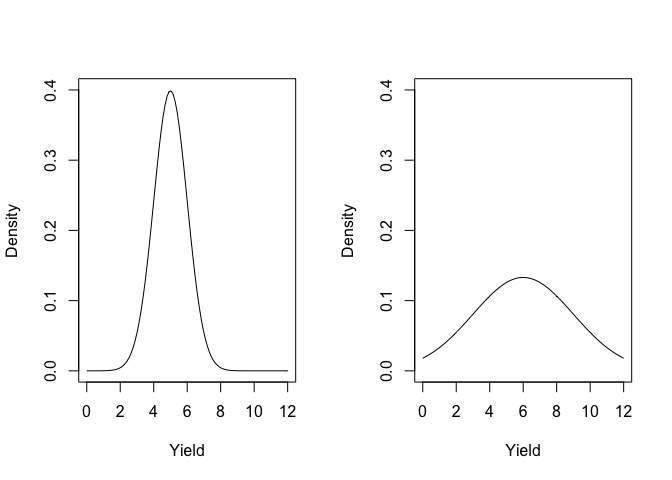
\includegraphics[width=0.9\linewidth]{_main_files/figure-latex/figName51-1} 

}

\caption{Distribuzioni normali con diversa media e deviazione standard (rispettivamente 5 e 1 a sinistra, 6 e 3 a destra}\label{fig:figName51}
\end{figure}

\begin{figure}

{\centering 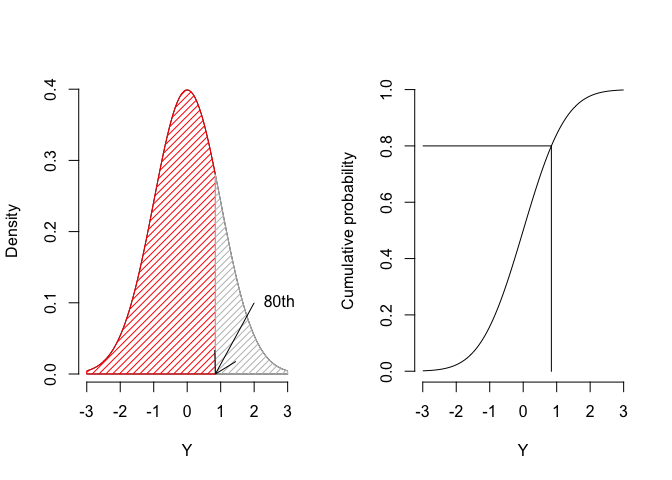
\includegraphics[width=0.9\linewidth]{_main_files/figure-latex/figName52-1} 

}

\caption{Integrale della curva di densità normale (80° percentile; sinistra) e curva di probabilità cumulata (destra)}\label{fig:figName52}
\end{figure}

\hypertarget{modelli-a-due-facce}{%
\section{Modelli `a due facce'}\label{modelli-a-due-facce}}

A questo punto, sempre in relazione al nostro frumento, possiamo scrivere che l'altezza della pianta \(i\) è:

\[Y_i = \mu + \varepsilon_i\]
dove abbiamo introdotto l'elemento stocastico \(\varepsilon\), per ogni soggetto \(i\), tale che:

\[ \varepsilon \sim N(0, \sigma) \]

cioè la componente stocastica \(\varepsilon\) è normalmente distribuita, con media 0 e deviazione standard \(\sigma\). E'abbastanza evidente che è possibile scrivere:

\[Y_i \sim N(\mu, \varepsilon)\]

cioè che l'altezza del frumento è normalmente distribuita con media \(\mu\) e deviazione standard \(\sigma\). Dato che si tratta di una semplice traslazione di una distribuzione normale lungo l'asse delle ascisse (come in figura @ref\{figName51\}), le due espressioni sono totalmente equivalenti.

Ora si può dire che conosciamo perfettamente la popolazione di partenza se conosciamo \(\mu\) e \(\sigma\), cioè la parte (`faccia') deterministica e la parte (`faccia') stocastica del modello. Se quindi immaginiamo che \(\mu = 100\) (come abbiamo detto in precedenza) e \(\sigma = 8\), possiamo risolvere alcuni semplici esercizi, utilizzando le funzioni di calcolo di probabilità di R.

\textbf{ESERCIZIO 1}. Calcolare la densità di un'altezza pari a 120 cm.

\begin{Shaded}
\begin{Highlighting}[]
\KeywordTok{dnorm}\NormalTok{(}\DecValTok{120}\NormalTok{, }\DataTypeTok{mean =} \DecValTok{100}\NormalTok{, }\DataTypeTok{sd =} \DecValTok{8}\NormalTok{)}
\CommentTok{## [1] 0.002191038}
\end{Highlighting}
\end{Shaded}

\textbf{ESERCIZIO 2}. Qual è la probabilità di ottenere piante con altezza inferiore a 80 cm?

\begin{Shaded}
\begin{Highlighting}[]
\KeywordTok{pnorm}\NormalTok{(}\DecValTok{80}\NormalTok{, }\DataTypeTok{mean =} \DecValTok{100}\NormalTok{, }\DataTypeTok{sd =} \DecValTok{8}\NormalTok{)}
\CommentTok{## [1] 0.006209665}
\end{Highlighting}
\end{Shaded}

\textbf{ESERCIZIO 3}. Qual è la probabilità di ottenere piante con altezza superiore a 110 cm?

\begin{Shaded}
\begin{Highlighting}[]
\KeywordTok{pnorm}\NormalTok{(}\DecValTok{110}\NormalTok{, }\DataTypeTok{mean =} \DecValTok{100}\NormalTok{, }\DataTypeTok{sd =} \DecValTok{8}\NormalTok{, }\DataTypeTok{lower.tail =}\NormalTok{ F)}
\CommentTok{## [1] 0.1056498}
\end{Highlighting}
\end{Shaded}

Si utilizza l'argomento lower.tail=FALSE, in quanto stiamo cercando la probabilità di un'a concentrazione pari o superiore ad 1.1, e non pari od inferiore.'altezza pari o superiore a 110 cm (upper-tail) e non quella pari o inferiore a 110 cm (lower-tail), che sarebbe fornita di default. E' totalmente equivalente utilizzare la funzione sottostante.

\begin{Shaded}
\begin{Highlighting}[]
\DecValTok{1} \OperatorTok{-}\StringTok{ }\KeywordTok{pnorm}\NormalTok{(}\DecValTok{110}\NormalTok{, }\DataTypeTok{mean =} \DecValTok{100}\NormalTok{, }\DataTypeTok{sd =} \DecValTok{8}\NormalTok{)}
\CommentTok{## [1] 0.1056498}
\end{Highlighting}
\end{Shaded}

\textbf{ESERCIZIO 4}. Qual è la probabilità di ottenere piante con altezza compresa tra 80 e 110 cm?

\begin{Shaded}
\begin{Highlighting}[]
\KeywordTok{pnorm}\NormalTok{(}\DecValTok{110}\NormalTok{, }\DataTypeTok{mean =} \DecValTok{100}\NormalTok{, }\DataTypeTok{sd =} \DecValTok{8}\NormalTok{) }\OperatorTok{-}\StringTok{ }\KeywordTok{pnorm}\NormalTok{(}\DecValTok{80}\NormalTok{, }\DataTypeTok{mean =} \DecValTok{100}\NormalTok{, }\DataTypeTok{sd =} \DecValTok{8}\NormalTok{)}
\CommentTok{## [1] 0.8881406}
\end{Highlighting}
\end{Shaded}

\textbf{ESERCIZIO 5}. Qual è quella misura che è superiore al 90\% di tutte le piante del campo (90° percentile?

\begin{Shaded}
\begin{Highlighting}[]
\KeywordTok{qnorm}\NormalTok{(}\FloatTok{0.9}\NormalTok{, }\DecValTok{100}\NormalTok{, }\DecValTok{8}\NormalTok{)}
\CommentTok{## [1] 110.2524}
\end{Highlighting}
\end{Shaded}

\textbf{ESERCIZIO 6}. Qual è quella misura che è inferiore al 20\% di tutte le piante del campo (80° percentile?

\begin{Shaded}
\begin{Highlighting}[]
\KeywordTok{qnorm}\NormalTok{(}\FloatTok{0.8}\NormalTok{, }\DecValTok{100}\NormalTok{, }\DecValTok{8}\NormalTok{)}
\CommentTok{## [1] 106.733}
\KeywordTok{qnorm}\NormalTok{(}\FloatTok{0.2}\NormalTok{, }\DecValTok{100}\NormalTok{, }\DecValTok{8}\NormalTok{, }\DataTypeTok{lower.tail=}\NormalTok{F)}
\CommentTok{## [1] 106.733}
\end{Highlighting}
\end{Shaded}

\textbf{ESERCIZIO 7}. Quali sono quei due valori, simmetrici rispetto alla media e tali da formare un intervallo all'interno del quale cadono il 95\% delle piante?

\begin{Shaded}
\begin{Highlighting}[]
\KeywordTok{qnorm}\NormalTok{(}\FloatTok{0.025}\NormalTok{, }\DecValTok{100}\NormalTok{, }\DecValTok{8}\NormalTok{)}
\CommentTok{## [1] 84.32029}
\KeywordTok{qnorm}\NormalTok{(}\FloatTok{0.975}\NormalTok{, }\DecValTok{100}\NormalTok{, }\DecValTok{8}\NormalTok{)}
\CommentTok{## [1] 115.6797}
\end{Highlighting}
\end{Shaded}

\hypertarget{e-allora}{%
\section{E allora?}\label{e-allora}}

Cerchiamo di ricapitolare. Le popolazioni di soggetti sperimentali e delle loro misure sono un oggetto largamente ignoto e inconoscibile. Infatti, le caratteristiche dei soggetti della popolazione sono, in parte, determinate in base a relazioni causa-effetto, ma, in altra parte, esse sono puramente stocastiche. Tuttavia è ragionevole supporre che esse seguano una qualche funzione di probabilità/densità (\textbf{assunzione parametrica}). Se questo è vero, allora possiamo utilizzare queste funzioni e i loro integrali per calcolare la probabilità di ottenere una certa misura o un certo insieme di misure.

\hypertarget{le-simulazioni-monte-carlo}{%
\section{Le simulazioni Monte Carlo}\label{le-simulazioni-monte-carlo}}

Se quanto abbiamo detto è vero, ogni esperimento scientifico non è altro che un'operazione di campionamento da una certa distribuzione di probabilità. Questo campionamento può essere simulato impiegando un generatore di numeri casuali. Immaginiamo di avere disegnato un esperimento con otto parcelle (repliche) per determinare la produzione del mais in un certo appezzamento e immaginiamo che queste parcelle costituiscano un campione rappresentativo della popolazione di parcelle di quell'appezzamento. Se la popolazione è distribuita normalmente, con media pari a 12 t/ha e deviazione standard pari ad 1.2 t/ha, allora possiamo simulare i risultati del nostro esperimento come segue:

\begin{Shaded}
\begin{Highlighting}[]
\KeywordTok{set.seed}\NormalTok{(}\DecValTok{1234}\NormalTok{)}
\NormalTok{Y <-}\StringTok{ }\KeywordTok{rnorm}\NormalTok{(}\DecValTok{8}\NormalTok{, }\DecValTok{15}\NormalTok{, }\FloatTok{1.2}\NormalTok{)}
\NormalTok{Y}
\CommentTok{## [1] 13.55152 15.33292 16.30133 12.18516 15.51495 15.60727 14.31031 14.34404}
\KeywordTok{mean}\NormalTok{(Y)}
\CommentTok{## [1] 14.64344}
\KeywordTok{sd}\NormalTok{(Y)}
\CommentTok{## [1] 1.328183}
\end{Highlighting}
\end{Shaded}

La generazione di numeri casuali con il computer viene fatta attraverso algoritmi che, a partire da un \emph{seed} iniziale, forniscono sequenze che obbediscono a certe proprietà fondamentali (numeri pseudo-casuali). Il comando `set.seed(1234)' ci permette di partire dallo stesso valore e quindi di ottenere lo stesso campione. Un'altra cosa da notare è che il nome della funzione che genara numeri casuali è formato con il nome della distribuzione (`norm') più il prefisso `r'. Questo è vero per tutte le altre distribuzioni in R (`rbinom', `rt' e così via)

I valori campionati non riflettono le caratteristiche della popolazione, nel senso che la media e la deviazione standard del campione differiscono da quelle della popolazione. E' esattamente ciò che capita durante un esperimento!

\hypertarget{analisi-dei-dati-e-model-fitting}{%
\section{Analisi dei dati e `model fitting'}\label{analisi-dei-dati-e-model-fitting}}

Secondo il principio illustrato in questo capitolo, un ricercatore arriverebbe a conoscere perfettamente la realtà se riuscisse ad individuare l'equazione e i parametri che governano il fenomeno in studio. Di conseguenza, l'ipotesi scientifica che sta alla base di un esperimento può essere posta sotto forma di modello matematico. Ad esempio, potremmo ipotizzare che la degradazione di un erbicida nel terreno segua una legge di decadimento esponenziale, rappresentabile, in genere, con l'equazione:

\[ C= a \, e^{-k T} + \varepsilon\]

dove \(C\) è la concentrazione dell'erbicida in un dato momento \(T\) ed \(a\) e \(k\) sono i parametri. Per quanto riguarda l'elemento stocastico, possiamo assumere che:

\[ \varepsilon \sim N(0, \sigma)\]

In modo equivalente, potremmo scrivere:

\[ C \sim N(a \, e^{-k T}, \sigma)\]

Questo modello è assolutamente generale; se vogliamo specificarlo per una certa situazione sperimentale, ad esempio per la degradazione di imazethapyr a 20°C, possiamo realizzare un esperimento nel quale contaminamo un terreno con questo erbicida, lo mettiamo a 20°C e, in tempi diversi, preleviamo aliquote di terreno da sottoporre a determinazione analitica. L'analisi dei dati raccolti consisterà nell'individuare \(a\), \(k\) e \(\sigma\), con una tecnica definita di \emph{model fitting}.

Le diverse tecniche di analisi dei dati che descriveremo nei capitoli successivi sono accomunate dall'essere appunto tecniche di \emph{model fitting}. Vedremo anche come queste tecniche possono essere utilizzate per verificare che le osservazioni sperimentali si conformino ad un dato modello (\emph{goodness of fit}) oppure per confrontare due ipotesi alternative poste sotto forma di modelli diversi (\emph{model comparison}).

\begin{center}\rule{0.5\linewidth}{\linethickness}\end{center}

\hypertarget{per-approfondire-un-po-2}{%
\section{Per approfondire un po'\ldots{}}\label{per-approfondire-un-po-2}}

\hypertarget{generazione-dei-dati-sperimentali-un-esempio-piu-realistico}{%
\subsection{Generazione dei dati sperimentali: un esempio più realistico}\label{generazione-dei-dati-sperimentali-un-esempio-piu-realistico}}

Immaginiamo di conoscere la legge deterministica che definisce la risposta del frumento alla concimazione azotata. In particolare, immaginiamo che questa risposta produttiva sia fondamentalmente lineare:

\[Y_E = b_0 + b_1 X\]

ed immaginiamo che, senza concimazione (X = 0), la produzione sia pari a 25 q/ha (\(b_0\) = 25). Immaginiamo che l'incremente produttivo per kg di azoto somministrato sia pari a 0.15 q/ha (\(b_1\) = 0.15).

Per individuare questa legge naturale organizziamo un esperimento, con quattro dosi di azoto e quattro repliche. In questo esperimento, come in tutti gli esperimenti, agirà anche una componente stocastica, che in qualche modo sposterà la risposta osservata dalla risposta attesa:

\[Y_o = b_0 + b_1 X + \varepsilon \quad \textrm{con}  \quad \varepsilon \sim N(0, \sigma)\]

Assumiamo che la componente stocastica \(\varepsilon\) sia distribuita normalmente, come media 0 e deviazione standard \(\sigma\), che immaginiamo essere pari a 2.5 q/ha.

Su questa base, generiamo i dati osservati, nelle seguenti fasi:

\begin{enumerate}
\def\labelenumi{\arabic{enumi}.}
\tightlist
\item
  generiamo i valori attesi (`Yield\_E'), utilizzando il modello deterministico di risposta. Le quattro repliche di una dose hanno, ovviamente, lo stesso valore;
\item
  aggiungiamo l'elemento stocastico, specifico per ogni osservazione, campionando da una distribuzione normale;
\item
  creiamo un dataframe con le osservazioni sperimentali
\end{enumerate}

\begin{Shaded}
\begin{Highlighting}[]
\KeywordTok{set.seed}\NormalTok{(}\DecValTok{1234}\NormalTok{)}
\NormalTok{Dose <-}\StringTok{ }\KeywordTok{rep}\NormalTok{(}\KeywordTok{c}\NormalTok{(}\DecValTok{0}\NormalTok{, }\DecValTok{60}\NormalTok{, }\DecValTok{120}\NormalTok{, }\DecValTok{180}\NormalTok{), }\DataTypeTok{each=}\DecValTok{4}\NormalTok{) }
\NormalTok{Yield_E <-}\StringTok{ }\DecValTok{25} \OperatorTok{+}\StringTok{ }\FloatTok{0.15} \OperatorTok{*}\StringTok{ }\NormalTok{Dose}
\NormalTok{epsilon <-}\StringTok{ }\KeywordTok{rnorm}\NormalTok{(}\DecValTok{16}\NormalTok{, }\DecValTok{0}\NormalTok{, }\FloatTok{2.5}\NormalTok{)}
\NormalTok{Yield <-}\StringTok{ }\NormalTok{Yield_E }\OperatorTok{+}\StringTok{ }\NormalTok{epsilon}
\NormalTok{dataset <-}\StringTok{ }\KeywordTok{data.frame}\NormalTok{(Dose, Yield)}
\NormalTok{dataset}
\CommentTok{##    Dose    Yield}
\CommentTok{## 1     0 21.98234}
\CommentTok{## 2     0 25.69357}
\CommentTok{## 3     0 27.71110}
\CommentTok{## 4     0 19.13576}
\CommentTok{## 5    60 35.07281}
\CommentTok{## 6    60 35.26514}
\CommentTok{## 7    60 32.56315}
\CommentTok{## 8    60 32.63342}
\CommentTok{## 9   120 41.58887}
\CommentTok{## 10  120 40.77491}
\CommentTok{## 11  120 41.80702}
\CommentTok{## 12  120 40.50403}
\CommentTok{## 13  180 50.05937}
\CommentTok{## 14  180 52.16115}
\CommentTok{## 15  180 54.39874}
\CommentTok{## 16  180 51.72429}
\CommentTok{# write.csv(dataset, file = "Nwheat.csv", row.names = F)}
\end{Highlighting}
\end{Shaded}

Il dataset che otteniamo è realistico e lo utilizzeremo per l'analisi (regressione lineare semplice) nel capitolo 12.

\hypertarget{modelli-stocastici-non-normali}{%
\subsection{Modelli stocastici non-normali}\label{modelli-stocastici-non-normali}}

Oltre alla distribuzione gaussiana, che è largamente la più importante, esistono molti altri modelli stocastici, sia per eventi continui che discreti. Chi volesse approfondire queste distribuzioni trova informazioni in seguito. Per gli altri vogliamo solo far notare che le funzioni di R per il calcolo di probabilità hanno sempre la stessa sintassi, che, dato il nome della distribuzione (es. `norm' per la distribuzione normale), assegna il prefisso `d' per la funzione di probabilità/densità, `p' per la funzione di probabilità cumulata, `q' per la funzione quantile. Ad esempio, per la distribuzione binomiale, il nome è `binom' e, di conseguenza, le funzioni in R sono: `dbinom()' (probabilità), `pbinom()' (probabilità cumulata) e `qbinom()' (funzione `quantile').

\hypertarget{t-di-student}{%
\subsubsection{t di Student}\label{t-di-student}}

La distribuzione t di Student è analoga, per forma, ad una distribuzione normale con media 0 e deviazione standard 1. Rispetto a quest'ultima, la dispersione è un po' più ampia, nel senso la probabilità di avere valori lontani dalla media è più alta. In realtà, non esiste una sola distribuzione t di Student, ma ne esistono molte, caratterizzate da un diverso numero di gradi di libertà (\(\nu\)); maggiore è \(\nu\), minore la sovradispersione; se il numero di gradi di libertà è infinito, la distribuzione t di Student è identica alla normale standardizzata (distribuzione normale con media 0 e deviazione standard uguale ad 1).

La Figura \ref{fig:figName2521} riporta un esempio di come diminuisce la sovradispersione all'aumentare del numero di gradi di libertà.

\begin{figure}

{\centering 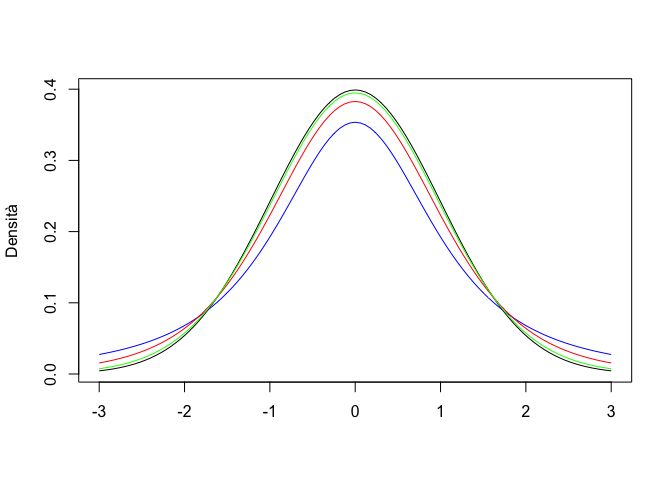
\includegraphics[width=0.9\linewidth]{_main_files/figure-latex/figName2521-1} 

}

\caption{Distribuzione t di Student, con diversi gradi di libertà}\label{fig:figName2521}
\end{figure}

\hypertarget{f-di-fisher}{%
\subsubsection{F di Fisher}\label{f-di-fisher}}

La distribuzione F di Fisher è definita solo per valori positivi ed è fortemente asimmetrica. Anche in questo caso, abbiamo una famiglia di distribuzioni, che differiscono tra di loro per due parametri (gradi di libertà) \(\nu_1\) e \(\nu_2\). Solitamente questa distribuzione viene utilizzata per descrivere il rapporto tra le varianze di coppie di campioni estratti da un distribuzione normale standardizzata, per cui \(\nu_1\) e \(\nu_2\) sono i gradi di libertà del numeratore e del denominatore.

La Figura \ref{fig:figName2522} mostra diverse funzioni di densità: possiamo notare come, all'aumentare dei gradi di libertà, la funzione F di Fisher tende ad assomigliare sempre di più ad una normale.

\begin{figure}

{\centering 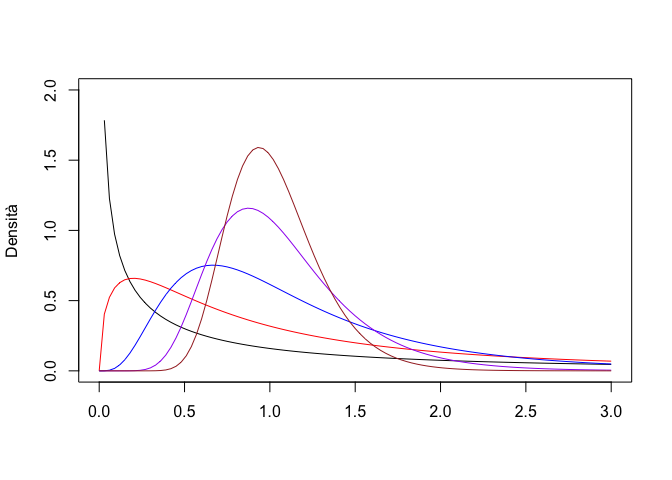
\includegraphics[width=0.9\linewidth]{_main_files/figure-latex/figName2522-1} 

}

\caption{Distribuzioni F di Fisher, con $
u_1 = 
u_2 = 
u$ e $
u = 1$ (linea nera), $
u = 3$ (linea rossa), $
u = 10$ (linea blues), $
u = 30$ (linea violetta) e $
u = 60$ (linea marrone)}\label{fig:figName2522}
\end{figure}

\hypertarget{la-distribuzione-binomiale}{%
\subsubsection{La distribuzione binomiale}\label{la-distribuzione-binomiale}}

Ogni esperimento per il quale ci siano solo due esiti possibili (successo ed insuccesso) e una certa probabilità di successo, viene detto \textbf{esperimento Bernoulliano}. Il tipico esempio è il lancio della moneta, nel quale possiamo ottenere solo testa o croce, con una probabilità di 0.5 (se la moneta non è truccata). In alcuni casi, potremmo avere una serie di esperimenti Bernoulliani indipendenti, con probabilità di successo costante (ad esempio, lanciare la moneta 10 volte) e potremmo essere interessati a conoscere la probabilità di ottenere \emph{k} successi su \emph{n} prove. Questa probabilità può essere descritta attraverso la \textbf{funzione di probabilità binomiale}.

Poniamo di sapere che in una Facoltà di Agraria con un numero molto elevato di studenti, il rapporto tra maschi e femmine sia pari a 0.7 e quindi che la probabilità di incontrare un maschio sia pari a \(p = 0.7\) (evento semplice). Deve essere estratto a sorte un viaggio studio per quattro studenti e, per una questione di pari opportunità, si preferirebbe che fossero premiati in ugual misura maschi e femmine (cioè si vogliono premiare due femmine). Qual è la probabilità che un simile evento si realizzi?

La probabilità cercata si può ottenere pensando che abbiamo un evento ``estrazione'' che può dare due risultati possibili (maschio o femmina) e che deve essere ripetuto quattro volte. Se consideriamo ``successo'' estrarre una femmina, allora la probabilità di successo in ogni estrazione è \(p = 0.3\) mentre quella di insuccesso (evento complementare) è pari a \(1 - p = q = 0.7\). Facciamo attenzione! Quanto abbiamo detto è vero solo se la popolazione è sufficientemente numerosa da pensare che la singola estrazione non cambia la probabilità degli eventi nelle successive (eventi indipendenti). La probabilità che su quattro estrazioni si abbiano 2 successi (due femmine) e due insuccessi (due maschi) è data da (teorema della probabilità composta):

\[0.3 \cdot 0.3 \cdot 0.7 \cdot 0.7 = 0.3^2 \cdot 0.7^2\]

In generale, data una popolazione molto numerosa, nella quale gli individui si presentano con due modalità possibili (in questo caso maschio e femmina) e posto di sapere che la frequenza con cui si presenta la prima modalità è pari a \(p\) (in questo caso la frequenza delle femmine è pari a 0.3), mentre la frequenza della seconda modalità è pari a \(q = 1 - p\), se vogliamo estrarre da questa popolazione \(n\) elementi, la probabilità che \(k\) di questi presentino la prima modalità (successo) è data da:

\[p^k \cdot q^{(n-k)}\]

La formula di cui sopra, tuttavia, non risolve il nostro problema, in quanto noi vogliamo che vengano estratte due femmine, indipendentemente dall'ordine con cui esse vengono estratte (prima, seconda, terza o quarta estrazione), mentre la probabilità che abbiamo appena calcolato è quella relativa all'evento in cui le due femmine sono estratte al primo e secondo posto.

Di conseguenza (teorema della probabilità totale), alla probabilità dell'evento indicato in precedenza (estrazione di due femmine in prima e seconda posizione) dobbiamo sommare la probabilità di tutti gli altri eventi utili (due femmine in seconda e terza posizione, oppure in terza e seconda, oppure in terza e quarta e così via). Il numero delle combinazioni possibili per 2 femmine in quattro estrazioni (combinazione di 4 elementi di classe 2) è dato dal coefficiente binomiale:

\[\left( {\begin{array}{*{20}c}
n  \\
k  \\
\end{array}} \right) = \frac{n!}{(n - k)!k!} \]

Moltiplicando le due equazioni date in precedenza otteniamo la funzione di probabilità binomiale:

\[P(X = x_i ) = \frac{{n!}}{{(n - k)!k!}} \cdot p^k \cdot q^{(n - k)} \]

Nel caso specifico otteniamo il risultato:

\[P(X = 2) = \frac{4!}{(4 - 2)!2!} \cdot 0.3^2 \cdot 0.7^{(4 - 2)}  = 0.2646 \]

che è appunto la probabilità cercata.

In R, utilizziamo la funzione `dbinom(successi, prove, probabilità semplice)' per calcolare la probabilità di ottenere \(k\) successi in \(n\) prove:

\begin{Shaded}
\begin{Highlighting}[]
\KeywordTok{dbinom}\NormalTok{(}\DecValTok{2}\NormalTok{, }\DecValTok{4}\NormalTok{, }\FloatTok{0.3}\NormalTok{)}
\CommentTok{## [1] 0.2646}
\end{Highlighting}
\end{Shaded}

La funzione binomiale è un modello stocastico e si può dimostrare che il valore atteso (media) è uguale ad \(n\cdot p\), mentre la varianza è pari a \(n\cdot p \cdot q\):

La funzione di ripartizione (probabilità cumulata) si calcola in R con la funzione `pbinom(successi, prove, probabilità semplice)'. Nell'esempio, se vogliamo sapere la probabilità totale di estrarre meno di tre femmine (2 femmine o meno), possiamo operare in questo modo:

\begin{Shaded}
\begin{Highlighting}[]
\KeywordTok{pbinom}\NormalTok{(}\DecValTok{2}\NormalTok{,}\DecValTok{4}\NormalTok{,}\FloatTok{0.3}\NormalTok{)}
\CommentTok{## [1] 0.9163}
\end{Highlighting}
\end{Shaded}

Che risulta anche dalla somma della probabilità di estrarre 0, 1, 2 femmine:

\begin{Shaded}
\begin{Highlighting}[]
\NormalTok{zero <-}\StringTok{ }\KeywordTok{dbinom}\NormalTok{(}\DecValTok{0}\NormalTok{,}\DecValTok{4}\NormalTok{,}\FloatTok{0.3}\NormalTok{)}
\NormalTok{uno <-}\StringTok{ }\KeywordTok{dbinom}\NormalTok{(}\DecValTok{1}\NormalTok{,}\DecValTok{4}\NormalTok{,}\FloatTok{0.3}\NormalTok{)}
\NormalTok{due <-}\StringTok{ }\KeywordTok{dbinom}\NormalTok{(}\DecValTok{2}\NormalTok{,}\DecValTok{4}\NormalTok{,}\FloatTok{0.3}\NormalTok{)}
\NormalTok{zero }\OperatorTok{+}\StringTok{ }\NormalTok{uno }\OperatorTok{+}\StringTok{ }\NormalTok{due}
\CommentTok{## [1] 0.9163}
\end{Highlighting}
\end{Shaded}

La funzione di ripartizione può anche essere utilizzata al contrario, per determinare i quantili, cioè il numero di successi che corrispondono ad una probabilità cumulata pari ad alfa:

\begin{Shaded}
\begin{Highlighting}[]
\KeywordTok{qbinom}\NormalTok{(}\FloatTok{0.9163}\NormalTok{,}\DecValTok{4}\NormalTok{,}\FloatTok{0.3}\NormalTok{)}
\CommentTok{## [1] 2}
\end{Highlighting}
\end{Shaded}

\hypertarget{altre-letture}{%
\subsection{Altre letture}\label{altre-letture}}

\begin{enumerate}
\def\labelenumi{\arabic{enumi}.}
\tightlist
\item
  Bolker, B.M., 2008. Ecological models and data in R. Princeton University Press, Books.
\item
  Schabenberger, O., Pierce, F.J., 2002. Contemporary statistical models for the plant and soil sciences. Taylor \& Francis, CRC Press, Books.
\end{enumerate}

\hypertarget{stime-ed-incertezza}{%
\chapter{Stime ed incertezza}\label{stime-ed-incertezza}}

Abbiamo già visto che un esperimento scientifico non è altro che un'operazione di campionamento, con la quale io, invece che studiare una popolazione enorme di soggetti, posso studiarne un gruppo sufficientemente piccolo, e compatibile con le mie limitate risorse di tempo e denaro. Anche se il campione estratto è effettivamente rappresentativo della popolazione, rimane il fatto che esso è il risultato di uno solo degli infiniti sforzi di campionamento possibili. Con due importanti conseguenze:

\begin{enumerate}
\def\labelenumi{\arabic{enumi}.}
\tightlist
\item
  le sue caratteristiche non necessariamente riflettono quelle della popolazione che lo ha generato;
\item
  campionamenti successivi forniscono risultati diversi, perché diversi sono i soggetti e, spesso, anche le condizioni in cui l'esperimento viene eseguito.
\end{enumerate}

Di conseguenza, al di là del campione, il nostro interesse rimane fondamentalmente rivolto verso la popolazione che lo ha generato. Ci dobbiamo chiedere quale sia la relazione tra le caratteristiche del campione e quelle della popolazione da cui esso è estratto. Questo processo logico prende il nome di \emph{inferenza statistica} e può essere condotto secondo le teorie di Karl Pearson (1857-1936), Egon Pearson (suo figlio: 1895-1980) e Jarzy Neyman (1894-1981), oltre al solito Ronald Fisher.

\hypertarget{lanalisi-dei-dati-gli-ingredienti-fondamentali}{%
\section{L'analisi dei dati: gli `ingredienti' fondamentali}\label{lanalisi-dei-dati-gli-ingredienti-fondamentali}}

Richiamiamo il percorso logico che abbiamo introdotto nel capitolo precedente:

\begin{enumerate}
\def\labelenumi{\arabic{enumi}.}
\tightlist
\item
  I fenomeni biologici seguono una legge di natura (verità `vera'), che ne costituisce il meccanismo deterministico fondamentale.
\item
  Quando si organizza un esperimento, i soggetti sperimentali obbediscono a questo meccanismo di fondo, al quale tuttavia si sovrappongono molto altri elementi di `confusione', altamente incontrollabili, che vanno sotto il nome di errore sperimentale.
\item
  L'osservazione sperimentale è quindi un'immagine confusa della verità vera e, soprattutto, l'osservazione sperimentale tende ad essere diversa per ogni sforzo di campionamento.
\item
  Compito del ricercatore è quello di separare l'informazione (che rappresenta la verità `vera') dal `rumore di fondo' provocato dall'errore sperimentale.
\end{enumerate}

Questo dualismo tra verità `vera' (inconoscibile) e verità sperimentale (esplorabile tramite un esperimento opportunamente pianificato) è l'aspetto centrale di tutta la biometria ed è schematizzato nella figura \ref{fig:figName61}. Di esso abbiamo fatto menzione più volte nei capitoli precedenti.

\begin{figure}

{\centering 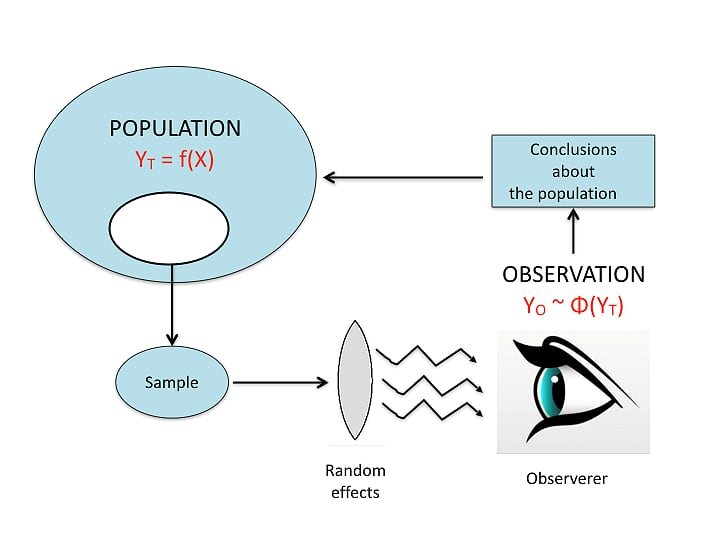
\includegraphics[width=0.75\linewidth]{_images/InferenceProcess} 

}

\caption{Osservazioni sperimentali e meccanismi perturbativi}\label{fig:figName61}
\end{figure}

In questo percorso logico ci sono due aspetti fondamentali che debbono essere attentamente valutati:

\begin{enumerate}
\def\labelenumi{\arabic{enumi}.}
\tightlist
\item
  modello di generazione dei dati sperimentali;
\item
  sampling distribution (o sample space).
\end{enumerate}

Chiariamo i due concetti con un esempio.

\hypertarget{esempio-una-soluzione-erbicida}{%
\section{Esempio: una soluzione erbicida}\label{esempio-una-soluzione-erbicida}}

Immaginiamo questa situazione: abbiamo una soluzione erbicida a concentrazione pari a 120 \(mg/l\), che viene misurata tramite un gascromatografo. Lo strumento di misura, unitamente a tutte le altre fonti ignote di errore, produce un coefficiente di variabilità del 10\% (corrispondente ad una deviazione standard pari a 12 \(mg/l\)). Facciamo le analisi in triplicato, come usuale per questo tipo di lavori.

\hypertarget{il-modello-dei-dati}{%
\subsection{Il modello dei dati}\label{il-modello-dei-dati}}

In primo luogo, ci chiediamo quale sia il modello matematico che genera le nostre osservazioni. Considerando quanto detto nel capitolo precedente, possiamo assumere che:

\[ Y_i = \mu + \varepsilon_i\]

dove:

\[ \varepsilon_i \sim N(\mu, \sigma)\]

cioè possiamo assumere che i risultati delle nostre misure siano normalmente distribuiti con media \(\mu = 120\) e deviazione standard \(\sigma = 12\).

Con queste informazioni possiamo simulare un esperimento con R, ottenendo i seguenti risultati:

\begin{Shaded}
\begin{Highlighting}[]
\KeywordTok{set.seed}\NormalTok{(}\DecValTok{1234}\NormalTok{)}
\NormalTok{Y <-}\StringTok{ }\KeywordTok{rnorm}\NormalTok{(}\DecValTok{3}\NormalTok{, }\DecValTok{120}\NormalTok{, }\DecValTok{12}\NormalTok{)}
\NormalTok{Y}
\CommentTok{## [1] 105.5152 123.3292 133.0133}
\end{Highlighting}
\end{Shaded}

\hypertarget{analisi-dei-dati-stima-dei-parametri}{%
\subsection{Analisi dei dati: stima dei parametri}\label{analisi-dei-dati-stima-dei-parametri}}

Nelle due equazioni sovrastanti, gli elementi incogniti sono \(\mu\) e \(\sigma\). In realtà, dato che si tratta di una simulazione, sappiamo che essi sono pari, rispettivamente, a 120 e 12; tuttavia, nella realtà questa informazione sarebbe totalmente sconosciuta. Guardando il campione, le nostre migliori stime \(\mu\) e \(\sigma\), che chiameremo rispettivamente \(m\) ed \(s\), sono pari rispettivamente alla media e alla deviazione standard del campione.

\begin{Shaded}
\begin{Highlighting}[]
\NormalTok{m <-}\StringTok{ }\KeywordTok{mean}\NormalTok{(Y)}
\NormalTok{s <-}\StringTok{ }\KeywordTok{sd}\NormalTok{(Y)}
\NormalTok{m; s}
\CommentTok{## [1] 120.6192}
\CommentTok{## [1] 13.9479}
\end{Highlighting}
\end{Shaded}

Questo processo con il quale assegniamo alla popolazione le caratteristiche del campione prende il nome di \textbf{stima puntuale} dei parametri. Vediamo ancora una volta che l'osservazione sperimentale non coincide con la verità `vera' (\(m \ne \mu\) e \(s \ne \sigma)\), ma non siamo molto distanti, considerando il 10\% di variabilità dello strumento di analisi. Tuttavia, visto che dobbiamo trarre conclusioni che riguardano la popolazione e non il campione, è giustificato da parte nostra un atteggiamento prudenziale: prima di dire che la concentrazione erbicida nella soluzione è pari 120.6192187, dobbiamo chiederci: che cosa succederebbe se ripetessimo l'esperimento molte altre volte?

\hypertarget{la-sampling-distribution}{%
\subsection{La `sampling distribution'}\label{la-sampling-distribution}}

In questo caso l'esperimento è solo `elettronico' e possiamo quindi ripeterlo un numero anche molto elevato di volte, seguendo questa procedura:

\begin{enumerate}
\def\labelenumi{\arabic{enumi}.}
\tightlist
\item
  Ripetiamo l'estrazione precedente per 100'000 volte (ripetiamo l'analisi chimica per 100'000 volte, sempre con tre repliche)
\item
  Otteniamo 100'000 medie
\item
  Calcoliamo la media delle medie e la deviazione standard delle medie
\end{enumerate}

\begin{Shaded}
\begin{Highlighting}[]
\CommentTok{# Simulazione MONTE CARLO - Esempio 1}
\KeywordTok{set.seed}\NormalTok{(}\DecValTok{1234}\NormalTok{)}
\NormalTok{result <-}\StringTok{ }\KeywordTok{rep}\NormalTok{(}\DecValTok{0}\NormalTok{, }\DecValTok{100000}\NormalTok{)}
\ControlFlowTok{for}\NormalTok{ (i }\ControlFlowTok{in} \DecValTok{1}\OperatorTok{:}\DecValTok{100000}\NormalTok{)\{}
\NormalTok{  sample <-}\StringTok{ }\KeywordTok{rnorm}\NormalTok{(}\DecValTok{3}\NormalTok{, }\DecValTok{120}\NormalTok{, }\DecValTok{12}\NormalTok{)}
\NormalTok{  result[i] <-}\StringTok{ }\KeywordTok{mean}\NormalTok{(sample)}
\NormalTok{\}}
\KeywordTok{mean}\NormalTok{(result)}
\CommentTok{## [1] 120.0341}
\KeywordTok{sd}\NormalTok{(result)}
\CommentTok{## [1] 6.939063}
\end{Highlighting}
\end{Shaded}

In sostanza, la simulazione Monte Carlo ci consente di fare quello che dovremmo sempre fare, cioè ripetere l'esperimento un numero di volte molto elevato, anche se finito (un numero infinito è chiaramente impossibile!). A questo punto abbiamo in mano una popolazione di medie, che viene detta \textbf{sampling distribution}, un `oggetto' abbastanza `teorico', ma fondamentale per la statistica frequentista, perché caratterizza la variabilità dei risultati di un esperimento, e quindi la sua riproducibilità.

Notiamo che:

\begin{enumerate}
\def\labelenumi{\arabic{enumi}.}
\tightlist
\item
  La media delle medie è praticamente coincidente con \(\mu\), la verità `vera'. Ciò conferma che l'unico modo di ottenere risultati totalmente precisi è ripetere infinite volte l'esperimento;
\item
  La deviazione standard delle medie è pari a 6.939063. Questo valore prende il nome di \textbf{errore standard} della media (SEM).
\end{enumerate}

Esploriamo meglio la \emph{sampling distribution}. Con R possiamo provare a discretizzarla e a riportarla su di un grafico a barre (figura \ref{fig:figName62} ).

\begin{figure}

{\centering 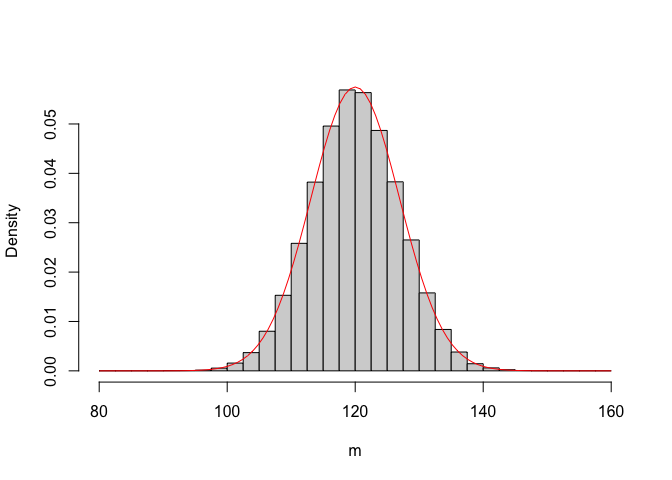
\includegraphics[width=0.9\linewidth]{_main_files/figure-latex/figName62-1} 

}

\caption{Sampling distribution empirica e teorica}\label{fig:figName62}
\end{figure}

\hypertarget{lerrore-standard}{%
\subsection{L'errore standard}\label{lerrore-standard}}

La \emph{sampling distribution} che abbiamo ottenuto con la simulazione Monte Carlo è puramente empirica. Sarebbe interessante capire con più esattezza se esista una funzione di densità che permetta di descriverla con esattezza. In effetti, il grafico precedente mostra che la \emph{sampling distribution} assomiglia molto ad una distribuzione normale, con media pari a 120 e deviazione standard pari all'errore standard.

Formalmente, il problema si può risolvere grazie alla legge di propagazione degli errori, che stabilisce tre importanti elementi:

\begin{enumerate}
\def\labelenumi{\arabic{enumi}.}
\tightlist
\item
  Se ho due variabili normalmente distribuite e le sommo tra di loro, la variabile risultante è ancora normale. Se ho una variabile normalmente distribuita e la moltiplico per una costante, la variabile risultante è ancora normale.
\item
  Per variabili indipendenti, la varianza della somma è uguale alla somma delle varianze.
\item
  La varianza del prodotto di una variabile per una costante \(k\) è pari alla varianza della variabile originale moltiplicata per \(k^2\).
\end{enumerate}

Consideriamo che, quando preleviamo alcuni individui da una popolazione, ognuno di essi porta con sé una sua componente di incertezza, che egli `eredita' dalla popolazione di cui fa parte. In questo caso, la popolazione ha una varianza pari a \(12^2 = 144\) e quindi ognuno dei tre soggetti campionati eredita tale varianza. Quando calcolo la media di tre osservazioni, in prima battuta io le sommo. A questo punto, dato che si tratta di osservazioni indipendenti, la propagazione degli errori (punto 2) ci dice che la varianza della somma è uguale a \(144 \times 3 = 432\).

Dopo aver sommato, il calcolo della media richiede che il risultato venga diviso per 3. La legge di propagazione degli errori (punto 3) ci dice quindi che la varianza viene divisa per \(3^2 = 9\). Insomma la popolazione delle medie è normale (punto 1), ha media pari a 120 e varianza pari a \(432/9 = 48\) e, di conseguenza, deviazione standard pari a \(\sqrt{48} = 6.928\), cioè \(12/\sqrt{3}\). In generale, l'errore standard di una media è:

\[\sigma_m  = \frac{\sigma }{\sqrt n }\]

dove \emph{n} è la dimensione del campione.

\hypertarget{riepilogo-1-caratterizzare-lincertezza-di-un-esperimento}{%
\section{Riepilogo 1: Caratterizzare l'incertezza di un esperimento}\label{riepilogo-1-caratterizzare-lincertezza-di-un-esperimento}}

Che cosa ci insegna questo esperimento? Ci insegna che, se prendiamo una distribuzione normale con media \(\mu\) e deviazione standard \(\sigma\) e cominciamo ad estrarre campioni, le medie dei campioni sono variabili, secondo una distribuzione normale con media \(\mu\) e deviazione standard \(\sigma / \sqrt{n}\). Questo concetto è interessante e può essere utilizzato per caratterizzare l'incertezza dei risultati di un esperimento. Riassumiamo:

\begin{enumerate}
\def\labelenumi{\arabic{enumi}.}
\tightlist
\item
  Abbiamo fatto un esperimento con tre repliche campionando da una distribuzione normale incognita.
\item
  Abbiamo ottenuto i tre valori 105.5152, 123.3292 e 133.0133.
\item
  In base alle osservazioni in nostro possesso, concludiamo che la concentrazione erbicida è pari a m = 120.6192 \(mg/l\), con una deviazione standard pari a 13.9479 \(mg/l\).
\item
  Dobbiamo adottare un atteggiamento prudenziale in relazione alla media, dato che non sappiamo il valore vero di \(\mu\).
\item
  Immaginiamo di conoscere la sampling distribution, che avrà una deviazione standard pari a:
\end{enumerate}

\begin{Shaded}
\begin{Highlighting}[]
\KeywordTok{sd}\NormalTok{(Y) }\OperatorTok{/}\StringTok{ }\KeywordTok{sqrt}\NormalTok{(}\DecValTok{3}\NormalTok{)}
\CommentTok{## [1] 8.052824}
\end{Highlighting}
\end{Shaded}

\begin{enumerate}
\def\labelenumi{\arabic{enumi}.}
\setcounter{enumi}{5}
\tightlist
\item
  Concludiamo quindi che \(\mu\) è pari a 120.6192 \(\pm\) 8.053
\end{enumerate}

Abbiamo caratterizzato l'incertezza del risultato attraverso un intervallo di valori (\textbf{stima per intervallo}).

\hypertarget{lintervallo-di-confidenza}{%
\section{L'intervallo di confidenza}\label{lintervallo-di-confidenza}}

Sarebbe interessante poter rispondere a questa domanda: ``qual è la proporzione di medie campionarie (cioè di ipotetici risultati del mio esperimento) che si trova all'interno della fascia di incertezza data?''. Un passo in avanti in questo senso è stato fatto da Neyman (1941), che propose di lavorare con la statistica T, definita come:

\[T = \frac{m - \mu}{\sigma_m}\]

dove \(\sigma_m\) è l'errore standard \(\sigma / \sqrt{n}\). Se \(m\) è distribuito normalmente con media \(\mu\) e deviazione standard \(\sigma\), la legge di propagazione degli errori ci dice che T è distribuito normalmente con media pari a \(m - \mu = 0\) e deviazione standard \(\sigma_m/\sigma_m = 1\). Cioè la \emph{sampling distribution} di T è una distribuzione normale standardizzata.\footnote{Tra tutte le distribuzioni normali, ce n'è una particolare, che ha media 0 e deviazione standard 1. Questa si chiama \textbf{distribuzione normale standardizzata}}

Quindi possiamo scrivere:

\[ P \left[ \textrm{qnorm}(0.025, 0, 1) \le \frac{m - \mu }{\sigma_m} \le \textrm{qnorm}(0.975, 0, 1) \right] = 0.95 \]

cioè: esiste una probabilità pari a 0.95 che \(T = (m - \mu)/\sigma_m\) è compreso tra il 2.5-esimo e il 97.5-esimo percentile di una distribuzione normale standardizzata. E' facile vedere che:

\begin{Shaded}
\begin{Highlighting}[]
\KeywordTok{qnorm}\NormalTok{(}\FloatTok{0.025}\NormalTok{, }\DecValTok{0}\NormalTok{, }\DecValTok{1}\NormalTok{)}
\CommentTok{## [1] -1.959964}
\KeywordTok{qnorm}\NormalTok{(}\FloatTok{0.975}\NormalTok{, }\DecValTok{0}\NormalTok{, }\DecValTok{1}\NormalTok{)}
\CommentTok{## [1] 1.959964}
\end{Highlighting}
\end{Shaded}

Quindi, approssimando alla seconda cifra decimale:

\[P \left[ -1.96 \le \frac{m - \mu }{\sigma_m} \le 1.96 \right] = 0.95\]

Con semplici passaggi algebrici, possiamo ottenere l'intervallo di confidenza:

\[P \left[ m -1.96 \times \sigma_m \le \mu \le m + 1.96 \times \sigma_m \right] = 0.95\]

Proviamo a leggere l'espressione sovrastante: se prendiamo la stima \(m\) e il suo errore standard \(\sigma_m\) e calcoliamo un intervallo di confidenza come 1.96 volte l'errore standard, \textbf{esiste una probabilità pari a 0.95 che questo intervallo contenga \(\mu\), cioè la media vera e ignota della popolazione}. In pratica, l'intervallo di confidenza potrebbe essere approssimato con il doppio dell'errore standard.

Il problema è che, nella pratica sperimentale, \(\sigma\) non è noto. Neyman propose di utilizzare \(s\) al posto di \(\sigma\), cioè la deviazione standard del campione, invece che quella della popolazione. Quindi, nel nostro caso, i limiti dell'intervallo di confidenza sono pari a:

\begin{Shaded}
\begin{Highlighting}[]
\NormalTok{m }\OperatorTok{+}\StringTok{ }\KeywordTok{qnorm}\NormalTok{(}\FloatTok{0.025}\NormalTok{) }\OperatorTok{*}\StringTok{ }\NormalTok{s}\OperatorTok{/}\KeywordTok{sqrt}\NormalTok{(}\DecValTok{3}\NormalTok{)}
\CommentTok{## [1] 104.836}
\NormalTok{m }\OperatorTok{+}\StringTok{ }\KeywordTok{qnorm}\NormalTok{(}\FloatTok{0.975}\NormalTok{) }\OperatorTok{*}\StringTok{ }\NormalTok{s}\OperatorTok{/}\KeywordTok{sqrt}\NormalTok{(}\DecValTok{3}\NormalTok{)}
\CommentTok{## [1] 136.4025}
\end{Highlighting}
\end{Shaded}

più semplicemente:

\begin{Shaded}
\begin{Highlighting}[]
\NormalTok{m }\OperatorTok{+}\StringTok{ }\DecValTok{2} \OperatorTok{*}\StringTok{ }\NormalTok{s}\OperatorTok{/}\KeywordTok{sqrt}\NormalTok{(}\DecValTok{3}\NormalTok{)}
\CommentTok{## [1] 136.7249}
\NormalTok{m }\OperatorTok{+}\StringTok{ }\DecValTok{2} \OperatorTok{*}\StringTok{ }\NormalTok{s}\OperatorTok{/}\KeywordTok{sqrt}\NormalTok{(}\DecValTok{3}\NormalTok{)}
\CommentTok{## [1] 136.7249}
\end{Highlighting}
\end{Shaded}

Questo che abbiamo calcolato è l'intervallo di confidenza per P = 0.95. Aumentando opportunamente il moltiplicatore possiamo calcolare gli intervalli di confidenza per P = 0.99, P = 0.999 e così via. Di fatto, l'intervallo di confidenza per P = 0.95 è il più utilizzato in pratica.

\hypertarget{qual-e-il-senso-dellintervallo-di-confidenza}{%
\section{Qual è il senso dell'intervallo di confidenza?}\label{qual-e-il-senso-dellintervallo-di-confidenza}}

E' utile ricordare il nostro punto di partenza e il nostro punto di arrivo:

\begin{enumerate}
\def\labelenumi{\arabic{enumi}.}
\tightlist
\item
  PUNTO DI PARTENZA: una distribuzione normale con \(\mu\) = 120 e \(\sigma\) = 12. Nella realtà assumiamo che la distribuzione di partenza sia normale, mentre i suoi parametri sono totalmente ignoti.
\item
  PUNTO DI ARRIVO: una stima di \(\mu\) ed un intervallo di confidenza.
\end{enumerate}

Che cosa significa questo intervallo? Esso fornisce:

\begin{enumerate}
\def\labelenumi{\arabic{enumi}.}
\tightlist
\item
  una misura di precisione: più piccolo è l'intervallo, maggiore è la precisione della stima;
\item
  un'espressione di confidenza nel fatto che, se ripetessimo molte volte l'esperimento, nel 95\% dei casi l'intervallo calcolato conterrebbe \(\mu\).
\end{enumerate}

Insomma, l'intervallo di confidenza serve ad esplicitare la nostra incertezza sulla media vera della popolazione in studio.

\hypertarget{come-presentare-i-risultati-degli-esperimenti}{%
\section{Come presentare i risultati degli esperimenti}\label{come-presentare-i-risultati-degli-esperimenti}}

Dopo aver letto questo capitolo e quelli precedenti, dovrebbe essere chiaro che la presenza dell'errore sperimentale crea incertezza in relazione alle caratteristiche della popolazione da cui abbiamo estratto il campione. Pertanto, è sempre obbligatorio associare alle nostre stime un indicatore di incertezza, la cui assenza non è, in linea di principio, accettabile. Possiamo considerare le seguenti possibilità:

\begin{enumerate}
\def\labelenumi{\arabic{enumi}.}
\tightlist
\item
  riportare la media associata alla deviazione standard, per descrivere la variabilità originale del fenomeno in studio;
\item
  riportare la media associata all'errore standard, per descrivere l'incertezza associata alla stima della media;
\item
  riportare l'intervallo di confidenza ottenuto sottraendo/aggiungendo alla media il doppio dell'errore standard, per descrivere l'incertezza associata alla stima della media;
\end{enumerate}

\hypertarget{alcune-precisazioni}{%
\section{Alcune precisazioni}\label{alcune-precisazioni}}

\hypertarget{campioni-numerosi-e-non}{%
\subsection{Campioni numerosi e non}\label{campioni-numerosi-e-non}}

Calcolare l'intervallo di confidenza utilizzando il doppio dell'errore standard costituisce un'approssimazione che è valida solo quando abbiamo esperimenti con un numero elevato di soggetti (maggiore di 15-20 circa). Per gli esperimenti piccoli, è necessario incrementare opportunamente il moltiplicatore. A questo fine viene utilizzato il valore corrispondente al 97.5-esimo percentile della distribuzione t di Student (non alla normale standardizzata, come abbiamo fatto finora), con un numero di gradi di libertà pari a quelli del campione studiato. Con tre soggetti il moltiplicatore sarebbe:

\begin{Shaded}
\begin{Highlighting}[]
\KeywordTok{qt}\NormalTok{(}\FloatTok{0.975}\NormalTok{, }\DecValTok{2}\NormalTok{)}
\CommentTok{## [1] 4.302653}
\end{Highlighting}
\end{Shaded}

Il moltiplicatore diminuisce all'aumentare della numerosità e, con 20 soggetti, diviene molto vicino a 2.

\begin{Shaded}
\begin{Highlighting}[]
\KeywordTok{qt}\NormalTok{(}\FloatTok{0.975}\NormalTok{, }\DecValTok{20}\NormalTok{)}
\CommentTok{## [1] 2.085963}
\end{Highlighting}
\end{Shaded}

Nel nostro esempio, con tre soggetti, l'intervallo di confidenza sarebbe:

\begin{Shaded}
\begin{Highlighting}[]
\NormalTok{m }\OperatorTok{+}\StringTok{ }\KeywordTok{qt}\NormalTok{(}\FloatTok{0.025}\NormalTok{, }\DecValTok{2}\NormalTok{) }\OperatorTok{*}\StringTok{ }\NormalTok{s}\OperatorTok{/}\KeywordTok{sqrt}\NormalTok{(}\DecValTok{3}\NormalTok{)}
\CommentTok{## [1] 85.97071}
\NormalTok{m }\OperatorTok{+}\StringTok{ }\KeywordTok{qt}\NormalTok{(}\FloatTok{0.975}\NormalTok{, }\DecValTok{2}\NormalTok{) }\OperatorTok{*}\StringTok{ }\NormalTok{s}\OperatorTok{/}\KeywordTok{sqrt}\NormalTok{(}\DecValTok{3}\NormalTok{)}
\CommentTok{## [1] 155.2677}
\end{Highlighting}
\end{Shaded}

Quindi, ben più alto di quello approssimato calcolato in precedenza. Chi ne volesse sapere di più, trova ulteriori informazioni in appendice.

\hypertarget{popolazioni-gaussiane-e-non}{%
\subsection{Popolazioni gaussiane e non}\label{popolazioni-gaussiane-e-non}}

In questo esempio siamo partiti da una popolazione con distribuzione gaussiana. In altri casi potrebbe non essere così. Ad esempio, immaginiamo di avere una popolazione di insetti, nella quale il rapporto tra maschi e femmine è ignoto. Campioniamo 40 insetti e contiamo 15 femmine. Qual è la proporzione di femmine nella popolazione originaria?

In questo caso stiamo studiando una grandezza che, almeno nel principio, non può essere gaussiana, ma è binomiale (vedi il capitolo precedente). Nonostante questo, possiamo utilizzare la stessa tecnica per la stima dell'intervallo di confidenza: sappiamo che la media di una distribuzione binomiale è \(p = 14/40 = 0.375\), mentre la deviazione standard è \(\sigma = \sqrt{0.375 \times (1 - 0.375)} = 0.484\). Di conseguenza, l'errore standard è \(0.484 / \sqrt{40} = 0.077\). L'intervallo di confidenza sarà dato quindi da:

\begin{Shaded}
\begin{Highlighting}[]
\FloatTok{0.375} \OperatorTok{-}\StringTok{ }\DecValTok{2} \OperatorTok{*}\StringTok{ }\FloatTok{0.077}
\CommentTok{## [1] 0.221}
\FloatTok{0.375} \OperatorTok{+}\StringTok{ }\DecValTok{2} \OperatorTok{*}\StringTok{ }\FloatTok{0.077}
\CommentTok{## [1] 0.529}
\end{Highlighting}
\end{Shaded}

Chi fosse interessato ad approfondire questi aspetti può proseguire nella lettura, dopo gli esercizi. Gli altri potranno fermarsi agli esercizi sottostanti.

\hypertarget{analisi-statistica-dei-dati-riassunto-del-percorso-logico}{%
\section{Analisi statistica dei dati: riassunto del percorso logico}\label{analisi-statistica-dei-dati-riassunto-del-percorso-logico}}

Considerando quanto finora detto, possiamo riassumere la logica dell'inferenza tradizionale nel modo seguente:

\begin{enumerate}
\def\labelenumi{\arabic{enumi}.}
\tightlist
\item
  Un esperimento è solo un campione di un numero infinito di esperimenti simili che avremmo potuto/dovuto eseguire, ma che non abbiamo eseguito, per mancanza di risorse;
\item
  Assumiamo che i dati del nostro esperimento sono generati da un modello matematico probabilistico, che prende una certa forma algebrica e ne stimiamo i parametri utilizzando i dati osservati;
\item
  Costruiamo la sampling distribution per i parametri stimati o per altre statistiche rilevanti, in modo da caratterizzare i risultati delle infinite repliche del nostro esperimento, che avremmo dovuto fare, ma che non abbiamo fatto.
\item
  Utilizziamo la sampling distribution per l'inferenza statistica.
\end{enumerate}

\hypertarget{da-ricordare}{%
\section{Da ricordare}\label{da-ricordare}}

\begin{enumerate}
\def\labelenumi{\arabic{enumi}.}
\tightlist
\item
  La natura genera i dati
\item
  Noi scegliamo un modello deterministico che simula il meccanismo di generazione dei dati attuato dalla natura.
\item
  Stimiamo i parametri.
\item
  Confrontiamo le previsioni con i dati osservati. Determiniamo \(\epsilon\) e la sua deviazione standard (\(\sigma\))
\item
  Assumiamo un modello stocastico ragionevole per spiegare \(\epsilon\), quasi sempre di tipo gaussiano, con media 0 e deviazione standard pari a \(\sigma\), indipendente dalla X (omoscedasticità)
\item
  Qualunque stima sperimentale deve essere associata ad un indicatore di variabilità (errore standard o intervallo di confidenza).
\end{enumerate}

\hypertarget{esercizi}{%
\section{Esercizi}\label{esercizi}}

\begin{enumerate}
\def\labelenumi{\arabic{enumi}.}
\tightlist
\item
  Un'analisi chimica è stata eseguita in triplicato, ottenendo i seguenti risultati: 125, 169 e 142 ng/g. Calcolare media, devianza, varianza, deviazione standard, coefficiente di variabilità ed errore standard.
\item
  Considerare il campione composto dai valori 140 - 170 - 155 e stimare i limiti di confidenza della media (P = 0.95).
\item
  Un campione di 400 insetti a cui è stato somministrato un certo insetticida mostra che 136 di essi sono sopravvissuti. Determinare un intervallo di confidenza con grado di fiducia del 95\% per la proporzione della popolazione insensibile al trattamento.
\end{enumerate}

\begin{center}\rule{0.5\linewidth}{\linethickness}\end{center}

\hypertarget{per-approfondire-un-po-3}{%
\section{Per approfondire un po'\ldots{}}\label{per-approfondire-un-po-3}}

\hypertarget{coverage-degli-intervalli-di-confidenza}{%
\section{\texorpdfstring{\emph{Coverage} degli intervalli di confidenza}{Coverage degli intervalli di confidenza}}\label{coverage-degli-intervalli-di-confidenza}}

Abbiamo visto che un metodo semplice per costruire un intervallo di confidenza è utilizzare il doppio dell'errore standard. Questo intervallo, se viene utilizzato come misura di precisione/incertezza, è sempre accettabile. Tuttavia, da un punto di vista strettamente probabilistico, è lecito chiedersi: ma è proprio vero che se io ripeto l'esperimento molte volte e calcolo sempre l'intervallo di confidenza, riesco a centrare la media \(\mu\) nel 95\% dei casi? È bene sapere che, con termine inglese, l'effettiva percentuale di campioni per i quali l'intervallo di confidenza, calcolato per un certo P nominale (es. P = 0.95), contiene effettivamente la media \(\mu\) della popolazione, viene detta \emph{coverage}. Quindi la nostra domanda è: qual è il \emph{coverage} dell'intervallo di confidenza calcolato con il doppio dell'errore standard?

Proviamo a rispondere a questa domanda con una simulazione Monte Carlo. Prendiamo la solita popolazione normalmente distribuita con \(\mu = 120\) e \(\sigma = 12\) ed estraiamo centomila campioni. Per ogni campione, calcoliamo l'intervallo di confidenza della media (P = 0.95) considerando il doppio dell'errore standard. Verifichiamo poi se questo intervallo contiene il valore 120: se si, assegniamo al campionamento il valore 1 (successo), altrimenti assegniamo il valore 0.

\begin{Shaded}
\begin{Highlighting}[]
\NormalTok{result <-}\StringTok{ }\KeywordTok{rep}\NormalTok{(}\DecValTok{0}\NormalTok{, }\DecValTok{100000}\NormalTok{)}
\KeywordTok{set.seed}\NormalTok{(}\DecValTok{1234}\NormalTok{)}
\ControlFlowTok{for}\NormalTok{ (i }\ControlFlowTok{in} \DecValTok{1}\OperatorTok{:}\DecValTok{100000}\NormalTok{)\{}
\NormalTok{  sample <-}\StringTok{ }\KeywordTok{rnorm}\NormalTok{(}\DecValTok{3}\NormalTok{, }\DecValTok{120}\NormalTok{, }\DecValTok{12}\NormalTok{)}
\NormalTok{  limInf<-}\StringTok{ }\KeywordTok{mean}\NormalTok{(sample) }\OperatorTok{-}\StringTok{ }\KeywordTok{sd}\NormalTok{(sample)}\OperatorTok{/}\KeywordTok{sqrt}\NormalTok{(}\DecValTok{3}\NormalTok{) }\OperatorTok{*}\StringTok{ }\DecValTok{2} 
\NormalTok{  limSup<-}\StringTok{ }\KeywordTok{mean}\NormalTok{(sample) }\OperatorTok{+}\StringTok{ }\KeywordTok{sd}\NormalTok{(sample)}\OperatorTok{/}\KeywordTok{sqrt}\NormalTok{(}\DecValTok{3}\NormalTok{) }\OperatorTok{*}\StringTok{ }\DecValTok{2}
  \ControlFlowTok{if}\NormalTok{ (limInf}\OperatorTok{<=}\StringTok{ }\DecValTok{120} \OperatorTok{&}\StringTok{ }\NormalTok{limSup}\OperatorTok{>=}\StringTok{ }\DecValTok{120}\NormalTok{) result[i] =}\StringTok{ }\DecValTok{1}
\NormalTok{\}}
\KeywordTok{sum}\NormalTok{(result)}\OperatorTok{/}\DecValTok{100000}
\CommentTok{## [1] 0.81708}
\end{Highlighting}
\end{Shaded}

La simulazione mostra che la risposta alla domanda precedente è no: il nostro intervallo di confidenza non è riuscito a centrare la media nel 95\% dei casi; ciò è avvenuto in poco più dell'80\% dei casi (\emph{coverage} dell 81.7\%, circa). In realtà, possiamo facilmente verificare, con altre simulazioni di Monte Carlo, che il \emph{coverage} si avvicina al 95\% solo se abbiamo campioni di numerosità superiore a 15-20 circa.

\begin{Shaded}
\begin{Highlighting}[]
\NormalTok{result <-}\StringTok{ }\KeywordTok{rep}\NormalTok{(}\DecValTok{0}\NormalTok{, }\DecValTok{100000}\NormalTok{)}
\KeywordTok{set.seed}\NormalTok{(}\DecValTok{1234}\NormalTok{)}
\ControlFlowTok{for}\NormalTok{ (i }\ControlFlowTok{in} \DecValTok{1}\OperatorTok{:}\DecValTok{100000}\NormalTok{)\{}
\NormalTok{  n <-}\StringTok{ }\DecValTok{15}
\NormalTok{  sample <-}\StringTok{ }\KeywordTok{rnorm}\NormalTok{(n, }\DecValTok{120}\NormalTok{, }\DecValTok{12}\NormalTok{)}
\NormalTok{  limInf<-}\StringTok{ }\KeywordTok{mean}\NormalTok{(sample) }\OperatorTok{-}\StringTok{ }\KeywordTok{sd}\NormalTok{(sample)}\OperatorTok{/}\KeywordTok{sqrt}\NormalTok{(n) }\OperatorTok{*}\StringTok{ }\DecValTok{2} 
\NormalTok{  limSup<-}\StringTok{ }\KeywordTok{mean}\NormalTok{(sample) }\OperatorTok{+}\StringTok{ }\KeywordTok{sd}\NormalTok{(sample)}\OperatorTok{/}\KeywordTok{sqrt}\NormalTok{(n) }\OperatorTok{*}\StringTok{ }\DecValTok{2}
  \ControlFlowTok{if}\NormalTok{ (limInf}\OperatorTok{<=}\StringTok{ }\DecValTok{120} \OperatorTok{&}\StringTok{ }\NormalTok{limSup}\OperatorTok{>=}\StringTok{ }\DecValTok{120}\NormalTok{) result[i] =}\StringTok{ }\DecValTok{1}
\NormalTok{\}}
\KeywordTok{sum}\NormalTok{(result)}\OperatorTok{/}\DecValTok{100000}
\CommentTok{## [1] 0.93594}
\end{Highlighting}
\end{Shaded}

Insomma, quando gli esperimenti sono piccoli, con poche repliche, dovremmo trovare un metodo di calcolo degli intervalli di confidenza un po' più affidabile, se veramente volessimo ottenere un \emph{coverage} pari a quello nominale (P = 0.95).

Il problema, già accennato, nasce dal fatto che \(\sigma_m\) viene sostituito con \(s_m\), cioè il valore di errore standard stimato nel campione. Come tutte le stime, anche \(s_m\) è soggetto ad incertezza, il che aggiunge un elemento ulteriore di imprecisione nella sampling distribution di \(T\). Insomma ci chiediamo, la \emph{sampling distribution} di T, calcolata con \(s\) invece che \(\sigma\) è ancora normale? Verifichiamo questo aspetto empiricamente, con una nuova simulazione Monte Carlo. Questa volta facciamo la seguente operazione:

\begin{enumerate}
\def\labelenumi{\arabic{enumi}.}
\tightlist
\item
  campioniamo tre individui
\item
  Calcoliamo il valore di \(T\) con la statistica precedente, utilizzando la deviazione standard del campione e lo salviamo
\item
  Con un po' di pazienza, ripetiamo il tutto 100'000 volte.
\end{enumerate}

\begin{Shaded}
\begin{Highlighting}[]
\CommentTok{#SIMULAZIONE MONTE CARLO - t di Student}
\KeywordTok{set.seed}\NormalTok{(}\DecValTok{435}\NormalTok{)}
\NormalTok{result <-}\StringTok{ }\KeywordTok{c}\NormalTok{()}
\ControlFlowTok{for}\NormalTok{ (i }\ControlFlowTok{in} \DecValTok{1}\OperatorTok{:}\DecValTok{100000}\NormalTok{)\{}
\NormalTok{  sample3 <-}\StringTok{ }\KeywordTok{rnorm}\NormalTok{(}\DecValTok{3}\NormalTok{, }\DecValTok{120}\NormalTok{, }\DecValTok{12}\NormalTok{)}
\NormalTok{  Ti <-}\StringTok{ }\NormalTok{(}\KeywordTok{mean}\NormalTok{(sample3) }\OperatorTok{-}\StringTok{ }\DecValTok{120}\NormalTok{) }\OperatorTok{/}\StringTok{ }\NormalTok{(}\KeywordTok{sd}\NormalTok{(sample3)}\OperatorTok{/}\KeywordTok{sqrt}\NormalTok{(}\DecValTok{3}\NormalTok{))}
\NormalTok{  result[i] <-}\StringTok{ }\NormalTok{Ti}
\NormalTok{  \}}
\end{Highlighting}
\end{Shaded}

Se riportiamo i valori ottenuti su una distribuzione di frequenze otteniamo il grafico in Figura \ref{fig:figName2531}.

\begin{Shaded}
\begin{Highlighting}[]
\NormalTok{b <-}\StringTok{ }\KeywordTok{seq}\NormalTok{(}\OperatorTok{-}\DecValTok{600}\NormalTok{, }\DecValTok{600}\NormalTok{, }\DataTypeTok{by=}\FloatTok{0.2}\NormalTok{)}
\KeywordTok{hist}\NormalTok{(result, }\DataTypeTok{breaks =}\NormalTok{ b, }\DataTypeTok{freq=}\NormalTok{F, }\DataTypeTok{xlab =} \KeywordTok{expression}\NormalTok{(}\KeywordTok{paste}\NormalTok{(m)), }\DataTypeTok{ylab=}\StringTok{"Density"}\NormalTok{, }\DataTypeTok{xlim=}\KeywordTok{c}\NormalTok{(}\OperatorTok{-}\DecValTok{10}\NormalTok{,}\DecValTok{10}\NormalTok{), }\DataTypeTok{ylim=}\KeywordTok{c}\NormalTok{(}\DecValTok{0}\NormalTok{,}\FloatTok{0.4}\NormalTok{), }\DataTypeTok{main=}\StringTok{""}\NormalTok{)}
\KeywordTok{curve}\NormalTok{(}\KeywordTok{dnorm}\NormalTok{(x, }\DecValTok{0}\NormalTok{, }\DecValTok{1}\NormalTok{), }\DataTypeTok{add=}\OtherTok{TRUE}\NormalTok{, }\DataTypeTok{col=}\StringTok{"blue"}\NormalTok{)}
\KeywordTok{curve}\NormalTok{(}\KeywordTok{dt}\NormalTok{(x, }\DecValTok{2}\NormalTok{), }\DataTypeTok{add=}\OtherTok{TRUE}\NormalTok{, }\DataTypeTok{col=}\StringTok{"red"}\NormalTok{)}
\end{Highlighting}
\end{Shaded}

\begin{figure}

{\centering 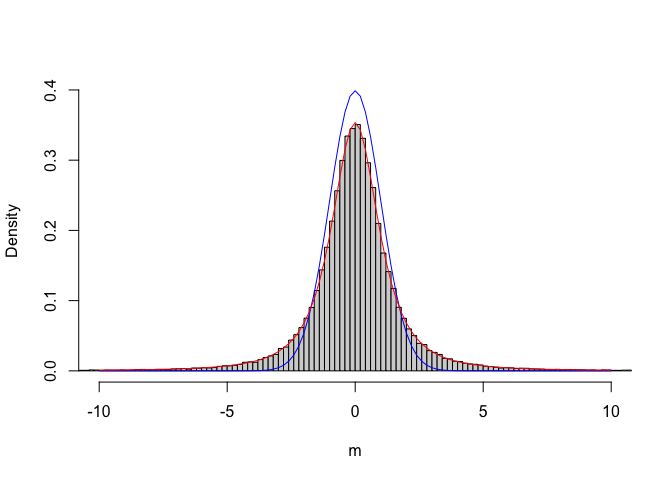
\includegraphics[width=0.9\linewidth]{_main_files/figure-latex/figName2531-1} 

}

\caption{Sampling distribution empirica per le medie campionarie, insieme ad una distribuzione gaussiana (blue) e t di Student con 2 gradi di libertà (rossa)}\label{fig:figName2531}
\end{figure}

Vediamo che la \emph{sampling distribution} di \(T\), determinata utilizzando \(s\) invece che \(\sigma\) è solo approssimativamente normale. E' facile vedere che questa approssimazione è sufficientemente buona solo se la numerosità del campione diviene abbastanza grande (es. \(n > 30)\), ma non certamente quando \(n\) = 3. In questo caso, la \emph{sampling distribution} che osserviamo è più `dispersa' di quella normale, con un maggior numero di valori sulle code.

Neyman scoprì che la sampling distribution di T poteva essere perfettamente descritta utilizzando la distribuzione t di Student, con un numero di gradi di libertà pari a quelli del campione (in questo caso 2), come vediamo nella figura \ref{fig:figName2531}. In realtà questa conclusione era stata già raggiunta da William Sealy Gosset (1876 - 1937), uno statistico impiegato presso la fabbrica londinese della famosa birra Guinness, dove elaborava i dati relativi all'andamento del processo di maltazione. Egli, avendo definito questa nuova funzione di densità, per aggirare il divieto di pubblicazione imposto dal suo datore di lavoro, pubblicò i risultati sotto lo pseudonimo Student, da cui deriva il nome della distribuzione di densità.

Quindi, quando i campioni sono piccoli, il modo giusto di calcolare l'intervallo di confidenza è quello di utilizzare l'espressione seguente:

\[P \left( m + \textrm{qt}(0.025,n - 1) \cdot s_m \le \mu  \le m + \textrm{qt}(0.975,n - 1) \cdot s_m \right) = 0.95\]

dove \(\textrm{qt}(0.025,n - 1)\) e \(\textrm{qt}(0.975,n - 1)\) sono rispettivamente il 2.5-esimo e il 97.5-esimo percentile della distribuzione t di Student, con n-1 gradi di libertà.

E' facile osservare che, se l'intervallo di confidenza è calcolato in questo modo, il suo \emph{coverage} effettivo e pari al 95\%.

\begin{Shaded}
\begin{Highlighting}[]
\NormalTok{result <-}\StringTok{ }\KeywordTok{rep}\NormalTok{(}\DecValTok{0}\NormalTok{, }\DecValTok{100000}\NormalTok{)}
\KeywordTok{set.seed}\NormalTok{(}\DecValTok{1234}\NormalTok{)}
\ControlFlowTok{for}\NormalTok{ (i }\ControlFlowTok{in} \DecValTok{1}\OperatorTok{:}\DecValTok{100000}\NormalTok{)\{}
\NormalTok{  sample <-}\StringTok{ }\KeywordTok{rnorm}\NormalTok{(}\DecValTok{3}\NormalTok{, }\DecValTok{120}\NormalTok{, }\DecValTok{12}\NormalTok{)}
\NormalTok{  limInf<-}\StringTok{ }\KeywordTok{mean}\NormalTok{(sample) }\OperatorTok{+}\StringTok{ }\KeywordTok{sd}\NormalTok{(sample)}\OperatorTok{/}\KeywordTok{sqrt}\NormalTok{(}\DecValTok{3}\NormalTok{) }\OperatorTok{*}\StringTok{ }\KeywordTok{qt}\NormalTok{(}\FloatTok{0.025}\NormalTok{, }\DecValTok{2}\NormalTok{) }
\NormalTok{  limSup<-}\StringTok{ }\KeywordTok{mean}\NormalTok{(sample) }\OperatorTok{+}\StringTok{ }\KeywordTok{sd}\NormalTok{(sample)}\OperatorTok{/}\KeywordTok{sqrt}\NormalTok{(}\DecValTok{3}\NormalTok{) }\OperatorTok{*}\StringTok{ }\KeywordTok{qt}\NormalTok{(}\FloatTok{0.975}\NormalTok{, }\DecValTok{2}\NormalTok{) }
  \ControlFlowTok{if}\NormalTok{ (limInf}\OperatorTok{<=}\StringTok{ }\DecValTok{120} \OperatorTok{&}\StringTok{ }\NormalTok{limSup}\OperatorTok{>=}\StringTok{ }\DecValTok{120}\NormalTok{) result[i] =}\StringTok{ }\DecValTok{1}
\NormalTok{\}}
\KeywordTok{sum}\NormalTok{(result)}\OperatorTok{/}\DecValTok{100000}
\CommentTok{## [1] 0.94936}
\end{Highlighting}
\end{Shaded}

Tuttavia, la formula di Neyman, anche se assicura un \emph{coverage} pari a quello nominale, si presta a cattive letture, che sono insensate da un punto di vista probabilistico, ma tuttavia molto frequenti nella pratica operativa. Ad esempio, immaginiamo di aver effettuato un campionamento dalla nostra popolazione con \(\mu = 120\) e \(\sigma = 12\). Il risultato è:

\begin{Shaded}
\begin{Highlighting}[]
\KeywordTok{set.seed}\NormalTok{(}\DecValTok{1234}\NormalTok{)}
\NormalTok{x <-}\StringTok{ }\KeywordTok{rnorm}\NormalTok{(}\DecValTok{3}\NormalTok{, }\DecValTok{120}\NormalTok{, }\DecValTok{12}\NormalTok{)}
\NormalTok{m <-}\StringTok{ }\KeywordTok{mean}\NormalTok{(x)}
\NormalTok{s <-}\StringTok{ }\KeywordTok{sd}\NormalTok{(x)}
\NormalTok{m; s}
\CommentTok{## [1] 120.6192}
\CommentTok{## [1] 13.9479}
\end{Highlighting}
\end{Shaded}

Di conseguenza, l'intervallo di confidenza va da 85.9707117 a 155.2677256

\begin{enumerate}
\def\labelenumi{\arabic{enumi}.}
\tightlist
\item
  \textbf{NON E' VERA} l'affermazione che: \emph{c'è il 95\% di probabilità che la media `vera' sia tra 85.0 e 155.3}. La media vera della popolazione è sempre fissa e pari a 120 e non cambia seguendo una distribuzione di probabilità. L'affermazione probabilistica deve essere riferita alla possibilità che l'intervallo di confidenza la centri, non al valore della media.
\item
  \textbf{E' DUBBIA} l'affermazione che: \emph{c'è il 95\% di probabilità che l'intervallo di confidenza contenga \(\mu\)}. In questa affermazione, la probabilità è legata all'intervallo di confidenza, ma l'affermazione è ugualmente sbagliata se si riferisce al singolo campionamento. Infatti, il singolo e specifico intervallo di confidenza (86.0 - 155.3) può contenere o no \(\mu\), ma non abbiamo alcun elemento per sapere se effittavamento lo contiene, neanche in termini di probabilità. Invece l'affermazione è corretta se si riferisce al futuro, cioè alle ipotetiche repliche dell'esperimento.
\item
  \textbf{NON E' VERA:} l'affermazione che \emph{ripetendo infinite volte l'esperimento, il 95\% delle stime che otteniamo cadono nell'intervallo 86.0 e 155.3}. Una semplice simulazione mostra che tutte le medie campionate cadono in quell'intervallo
\end{enumerate}

\begin{Shaded}
\begin{Highlighting}[]
\NormalTok{result <-}\StringTok{ }\KeywordTok{rep}\NormalTok{(}\DecValTok{0}\NormalTok{, }\DecValTok{100000}\NormalTok{)}
\KeywordTok{set.seed}\NormalTok{(}\DecValTok{1234}\NormalTok{)}
\ControlFlowTok{for}\NormalTok{ (i }\ControlFlowTok{in} \DecValTok{1}\OperatorTok{:}\DecValTok{100000}\NormalTok{)\{}
\NormalTok{  sample <-}\StringTok{ }\KeywordTok{rnorm}\NormalTok{(}\DecValTok{3}\NormalTok{, }\DecValTok{120}\NormalTok{, }\DecValTok{12}\NormalTok{)}
  \ControlFlowTok{if}\NormalTok{ (}\KeywordTok{mean}\NormalTok{(sample) }\OperatorTok{<=}\StringTok{ }\FloatTok{155.0} \OperatorTok{&}\StringTok{ }\KeywordTok{mean}\NormalTok{(sample) }\OperatorTok{>=}\StringTok{ }\FloatTok{85.3}\NormalTok{) result[i] =}\StringTok{ }\DecValTok{1}
\NormalTok{\}}
\KeywordTok{sum}\NormalTok{(result)}\OperatorTok{/}\DecValTok{100000}
\CommentTok{## [1] 1}
\end{Highlighting}
\end{Shaded}

Insomma, l'intervallo di confidenza vale per la sampling distribution e non vale per ogni singolo campionamento (esperimento). L'unica cosa che possiamo lecitamente affermare è che, se ripetessimo l'esperimento un numero molto elevato di volte e calcolassimo l'intervallo di confidenza sempre con la formula di Neyman, nel 95\% dei casi saremmo in grado di `catturare' la media vera della popolazione all'interno del nostro intervallo di confidenza, che diviene in questo modo una sorta di polizza assicurativa, per contenere la nostra probabilità d'errore, nel lungo periodo, al disotto del 5\%.

\hypertarget{intervalli-di-confidenza-per-fenomeni-non-normali}{%
\subsection{Intervalli di confidenza per fenomeni non-normali}\label{intervalli-di-confidenza-per-fenomeni-non-normali}}

Nel sottocapitolo precedente abbiamo presentato un esempio in cui avevamo campionato da una distribuzione normale, riscontrando una \emph{sampling distribution} per la media campionaria anch'essa normale (almeno approssimativamente). Ma che succede se la distribuzione di partenza è non-normale? La \emph{sampling distribution} di uno stimatore è ancora normale? Vediamo un nuovo esempio.

Immaginiamo di avere 4'000'000 di semi ben mischiati (in modo che non ci siano raggruppamenti non casuali di qualche tipo), che costituiscono la nostra popolazione di partenza. Vogliamo appurare la frequenza relativa (p) dei semi dormienti. Questa informazione, nella realtà, esiste (\(\pi\) = 0.25), ma non è nota.

Dato l'elevato numero di `soggetti', non possiamo testare la germinabilità di tutti i semi, ma dobbiamo necessariamente prelevare un campione casuale di 40 soggetti; ogni seme viene saggiato e, dato che la popolazione è molto numerosa, l'estrazione di un seme non modifica sensibilmente la proporzione di quelli dormienti nella popolazione (esperimenti indipendenti).

Dopo aver descritto la popolazione e l'esperimento, ci chiediamo quale sia il modello matematico che genera i nostri dati (numero di successi su 40 semi estratti). Il disegno sperimentale ci assicura che ogni estrazione è totalmente indipendente dalla precedente e dalla successiva ed ha due soli risultati possibili, cioè successo (seme dormiente), o insuccesso (seme germinabile). Di conseguenza, ogni singola estrazione si configura come un esperimento Bernoulliano, con probabilità di successo pari a \(\pi\), il cui valore `vero' esiste, è fisso, pre-determinato (esiste ancor prima di organizzare l'esperimento), anche se incognito e inconoscibile, a meno di non voler/poter esaminare tutti i semi disponibili. L'insieme delle 40 estrazioni (40 esperimenti Bernoulliani) può produrre un ventaglio di risultati possibili, da 40 successi a 40 insuccessi, per un totale di 41 possibili `outcomes'.

E' evidente che i 41 possibili risultati non sono ugualmente probabili e si può dimostrare che la probabilità di ottenere \emph{k} successi (con \emph{k} che va da 0 ad \emph{n}; \emph{n} è al numero delle estrazioni) dipende da \(\pi\) ed è descrivibile matematicamente con la distribuzione binomiale \(\phi\):

\[\phi(k, n, p) = \frac{n!}{(n-k)!k!} p^k (1 - p)^{(n-k)}\]

Abbiamo quindi definito il modello matematico che descrive la probabilità di tutti i possibili risultati del nostro esperimento e quindi può in qualche modo essere considerato il `meccanismo' che `genera' i dati sperimentali osservati. Si tratta di un meccanismo puramente `stocastico' nel quale è solo il caso che, attraverso il campionamento, determina il risultato dell'esperimento.

Con queste informazioni, possiamo simulare un esperimento con R, ottenendo i seguenti risultati:

\begin{Shaded}
\begin{Highlighting}[]
\KeywordTok{set.seed}\NormalTok{(}\DecValTok{236}\NormalTok{)}
\KeywordTok{rbinom}\NormalTok{(}\DecValTok{1}\NormalTok{, }\DecValTok{40}\NormalTok{, }\FloatTok{0.25}\NormalTok{)}
\CommentTok{## [1] 9}
\end{Highlighting}
\end{Shaded}

Abbiamo ottenuto 9 successi su 40, cioè 9 semi dormienti su 40 saggiati.La proporzione osservata è \emph{p} = 9/40 = 0.225. Concludiamo (stima puntuale) che \(\pi\) = 0.225. Anche in questo caso vi è chiara discrasia tra la verità `vera' e l'osservazione sperimentale (tra \(\pi\) e \(p\)).

Cosa succede se ripetiamo l'esperimento? Come abbiamo imparato a fare, possiamo cercare una risposta attraverso la simulazione Monte Carlo, ricorrendo ad un generatore di numeri casuali da una distribuzione binomiale con n = 40 e \(\pi\) = 0.25 (in R si usa la funzione `rbinom(numeroDatiCasuali, n, p)'). Il codice è più semplice, in quanto non è necessario impostare un ciclo iterativo:

\begin{Shaded}
\begin{Highlighting}[]
\KeywordTok{set.seed}\NormalTok{(}\DecValTok{1234}\NormalTok{)}
\NormalTok{result <-}\StringTok{ }\KeywordTok{rbinom}\NormalTok{(}\DecValTok{10000000}\NormalTok{, }\DecValTok{40}\NormalTok{, }\FloatTok{0.25}\NormalTok{)}
\end{Highlighting}
\end{Shaded}

Esploriamo i risultati ottenuti:

\begin{Shaded}
\begin{Highlighting}[]
\NormalTok{result_p <-}\StringTok{ }\NormalTok{result}\OperatorTok{/}\DecValTok{40}
\KeywordTok{mean}\NormalTok{(result_p)}
\CommentTok{## [1] 0.2499795}
\KeywordTok{sd}\NormalTok{(result_p)}
\CommentTok{## [1] 0.06849423}
\end{Highlighting}
\end{Shaded}

Osserviamo subito che, anche se i singoli esperimenti portano a stime diverse da \(\pi\) vero, la media di \(p\) tende ad essere uguale a \(\pi\). L'errore standard (deviazione standard della \emph{sampling distribution}) è 0.0685. Fino a qui, non vi è nulla di diverso dall'esempio precedente, se teniamo presente che la deviazione standard della popolazione originale (che è binomiale) è pari a \(\sqrt{p \times (1 - p)}\), quindi l'errore standard è \(\sqrt{0.25 \times 0.75 / 40} = 0.0685\).

Rimane da stabilire se la \emph{sampling distribution} di \(p\) è normale. Possiamo utilizzare i 10'000'000 di valori ottenuti per costruire una distribuzione empirica di frequenze, come nel codice sottostante.

\begin{Shaded}
\begin{Highlighting}[]
\NormalTok{breaks <-}\StringTok{ }\KeywordTok{seq}\NormalTok{(}\DecValTok{0}\NormalTok{, }\FloatTok{0.7}\NormalTok{, }\DataTypeTok{by=}\FloatTok{0.025}\NormalTok{)}
\NormalTok{freqAss <-}\StringTok{ }\KeywordTok{as.numeric}\NormalTok{( }\KeywordTok{table}\NormalTok{(}\KeywordTok{cut}\NormalTok{(result_p, breaks) ) ) }
\NormalTok{freqRel <-}\StringTok{ }\NormalTok{freqAss}\OperatorTok{/}\KeywordTok{length}\NormalTok{(result_p)}
\NormalTok{density <-}\StringTok{ }\NormalTok{freqRel}\OperatorTok{/}\FloatTok{0.025}
\NormalTok{p_oss <-}\StringTok{ }\NormalTok{breaks[}\DecValTok{2}\OperatorTok{:}\KeywordTok{length}\NormalTok{(breaks)]}
\end{Highlighting}
\end{Shaded}

La distribuzione empirica della proporzione campionaria è visibile in Figura @rif(fig:figName2541).

\begin{Shaded}
\begin{Highlighting}[]
\KeywordTok{plot}\NormalTok{(density }\OperatorTok{~}\StringTok{ }\NormalTok{p_oss, }\DataTypeTok{type =} \StringTok{"h"}\NormalTok{,}
     \DataTypeTok{xlab =} \KeywordTok{expression}\NormalTok{(}\KeywordTok{paste}\NormalTok{(}\KeywordTok{bar}\NormalTok{(p))),}
     \DataTypeTok{ylab=}\StringTok{"Density"}\NormalTok{, }
    \DataTypeTok{xlim=}\KeywordTok{c}\NormalTok{(}\DecValTok{0}\NormalTok{,}\FloatTok{0.6}\NormalTok{) )}
\NormalTok{b <-}\StringTok{ }\KeywordTok{seq}\NormalTok{(}\DecValTok{0}\NormalTok{, }\DecValTok{1}\NormalTok{, }\DataTypeTok{by=}\FloatTok{0.1}\NormalTok{)}
\KeywordTok{curve}\NormalTok{(}\KeywordTok{dnorm}\NormalTok{(x, }\FloatTok{0.25}\NormalTok{, }\FloatTok{0.0685}\NormalTok{), }\DataTypeTok{add=}\OtherTok{TRUE}\NormalTok{, }\DataTypeTok{col=}\StringTok{"red"}\NormalTok{)}
\end{Highlighting}
\end{Shaded}

\begin{figure}

{\centering 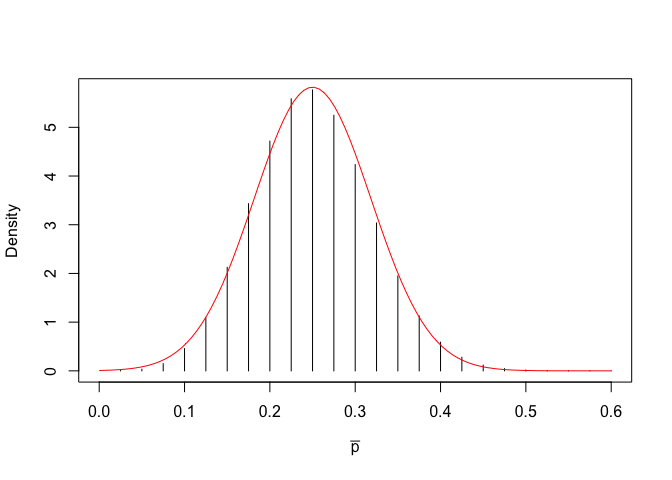
\includegraphics[width=0.9\linewidth]{_main_files/figure-latex/figName2541-1} 

}

\caption{Sampling distribution per le proporzioni campionarie}\label{fig:figName2541}
\end{figure}

Vediamo che \emph{sampling distribution} è approssimativamente normale con media pari a 0.25 e deviazione standard pari a 0.0685. Lo percepiamo chiaramente dal grafico soprastante, ma c'è una spiegazione scientifica per questo, basata sul \textbf{TEOREMA DEL LIMITE CENTRALE}:

\begin{enumerate}
\def\labelenumi{\arabic{enumi}.}
\tightlist
\item
  La sampling distribution di una statistica ottenuta da campioni casuali e indipendenti è approssimativamente normale, indipendentemente dalla distribuzione della popolazione da cui i campioni sono stati estratti.
\item
  La media della sampling distribution è uguale al valore della statistica calcolata sulla popolazione originale, la deviazione standard della sampling distribution (errore standard) è pari alla deviazione standard della popolazione originale divisa per la radice quadrata della numerosità di un campione.
\end{enumerate}

\hypertarget{altre-letture-1}{%
\subsection{Altre letture}\label{altre-letture-1}}

\begin{enumerate}
\def\labelenumi{\arabic{enumi}.}
\tightlist
\item
  Hastie, T., Tibshirani, R., Friedman, J., 2009. The elements of statistical learning, Springer Series in Statistics. Springer Science + Business Media, California, USA.
\end{enumerate}

\hypertarget{decisioni-e-incertezza}{%
\chapter{Decisioni e incertezza}\label{decisioni-e-incertezza}}

Nel capitolo precedente abbiamo visto come è possibile esprimere l'incertezza che il campionamente e, in genere, l'errore sperimentale producono sulle nostre stime. In particolare, abbiamo visto che, per una certa statistica rilevata su un campione, è possibile utilizzare la \emph{sampling distribution} (o \emph{sample space} o \emph{distribuzione campionaria}), con un procedimento che prende il nome di inferenza statistica (stima per intervallo). Analogamente, la \emph{sampling distribution} può essere utilizzata per prendere decisioni in presenza di incertezza, con un procedimento che si chiama test d'ipotesi. Anche in questo capitolo, vediamo alcuni esempi, partendo da quello già esposto in precedenza.

\hypertarget{confronto-tra-una-media-osservata-e-una-media-teorica}{%
\section{Confronto tra una media osservata e una media teorica}\label{confronto-tra-una-media-osservata-e-una-media-teorica}}

Nel capitolo precedente, abbiamo misurato la concentrazione di una soluzione erbicida tramite un gascromatografo. Facendo l'analisi in triplicato, abbiamo ottenuto i tre valori riportati di seguito.

\begin{verbatim}
## [1] 105.5152 123.3292 133.0133
\end{verbatim}

Abbiamo calcolato la media, la deviazione standard, l'errore standard e l'intervallo di confidenza. Ora immaginiamo che esista un livello soglia pari a 200 mg/l, al disopra del quale il prodotto diviene tossico per i mammiferi. Dato che non conosciamo il vero valore di \(\mu\) ci chiediamo: \emph{è possibile che le nostre tre repliche, nella realtà, provengano da una popolazione che ha media uguale a 200}?

In questo caso sappiamo bene che non è possibile, visto che abbiamo generato i dati sperimentali (vedi il capitolo precedente), tramite simulazione Monte Carlo, partendo da una verità vera nota (\(\mu\) = 120 e \(\sigma\) = 12); tuttavia, nella realtà, la domanda è lecita.

Potremmo formalizzare la nostra domanda mediante un'ipotesi scientifica, detta \emph{ipotesi nulla} (\(H_0\)), per la quale assumiamo che \(\mu = 200\). Scriviamo:

\[H_0: \mu = 200\]

Cerchiamo ora di vedere quanto la nostra osservazione è `discrepante' rispetto all'ipotesi nulla.

In particolare, possiamo calcolare una statistica, che abbiamo già utilizzato per l'intervallo di confidenza, in grado di misurare questa discrepanza:

\[ T = \frac{m - 200}{s_m} \]

Il valore da noi osservato è:

\begin{Shaded}
\begin{Highlighting}[]
\NormalTok{Ti <-}\StringTok{ }\NormalTok{(m }\OperatorTok{-}\StringTok{ }\DecValTok{200}\NormalTok{)}\OperatorTok{/}\NormalTok{sm}
\NormalTok{Ti}
\CommentTok{## [1] -9.857508}
\end{Highlighting}
\end{Shaded}

il che implica un certo grado di discrepanza, altrimenti avremmo dovuto osservare un valore di T più vicino a 0. \textbf{Possiamo affermare che ciò sia imputabile solo alla variabilità di campionamento e che quindi il nostro esperimento confermi l'ipotesi nulla (\(\mu = 200\))}?

È evidente che l'ipotesi nulla, oltre che come l'abbiamo scritta più sopra, potrebbe anche essere posta come:

\[H_0: T = 0\]

Oltre all'ipotesi nulla, dobbiamo anche definire l'ipotesi alternativa semplice (a `due code'), che potrebbe essere:

\[H_1: T \neq 0\]

E'possibile anche definire ipotesi alternative complesse del tipo:

\[H_1: T < 0\]

oppure:

\[H_1: T > 0\]

Bisogna ricordare che le ipotesi debbono essere stabilite prima di effettuare l'esperimento. In questo caso abbiamo fatto un campionamento e abbiamo trovato un valore (120.619) inferiore a quello atteso (200). Che cosa ci attendevamo prima di fare l'esperimento? Ci attendevamo un valore diverso da 200, ma non avevamo informazioni per immaginare se avrebbe potuto essere maggiore o minore? In questo caso l'ipotesi alternativa dovrebbe essere la prima (quella semplice). Avevamo invece ragionevoli motivi per ritenere che \(m\) avrebbe potuto essere inferiore, ma non superiore a 200? In questo caso l'ipotesi alternativo potrebbe essere la seconda (ipotesi alternativa complessa). Propendiamo per quest'ultima ipotesi, cioè \(\mu < 200\).

Siamo in totale coerenza con la logica Galileiana: abbiamo un ipotesi di partenza e un esperimento, col quale eventualmente rigettare questa ipotesi ,per abbracciarno una alternativa. Fisher, negli anni 20 del 1900, propose di utilizzare come \textbf{`forza dell'evidenza scientifica' la probabilità di ottenere un risultato uguale o più estremo di quello osservato, calcolato supponendo vera l'ipotesi nulla.} Penso che il modo migliore di spiegare questo concetta è attraverso l'esempio pratico.

\hypertarget{simulazione-monte-carlo}{%
\subsection{Simulazione Monte Carlo}\label{simulazione-monte-carlo}}

Supponiamo che l'ipotesi nulla sia vera. È evidente che, se prendiamo una popolazione gaussiana con \(\mu = 200\), cominciamo ad estrarre campioni e, per ognuno di essi, calcoliamo T, otterremo un 'ventaglio di valori, che danno origine ad una \emph{sampling distribution}. Ci chiediamo: come è fatta questa \emph{sampling distribution}?

La cosa migliore è costruirla con una simulazione Monte Carlo, ripetendo molte volte (es. 100'000) l'estrazione di campioni con numerosità pari a 3, da una distribuzione normale con media pari a 200 e deviazione standard pari a 13.948. Utilizziamo questo valore di deviazione standard perché è quello osservato nel campione e, nella realtà, sarebbe l'unico valore disponibile, dato che non sapremmo nulla della popolazione originale. Per eseguire questa operazione utilizziamo il seguente codice R:

\begin{Shaded}
\begin{Highlighting}[]
\KeywordTok{set.seed}\NormalTok{(}\DecValTok{1234}\NormalTok{)}
\NormalTok{result <-}\StringTok{ }\KeywordTok{rep}\NormalTok{(}\DecValTok{0}\NormalTok{, }\DecValTok{100000}\NormalTok{)}
\ControlFlowTok{for}\NormalTok{ (i }\ControlFlowTok{in} \DecValTok{1}\OperatorTok{:}\DecValTok{100000}\NormalTok{)\{}
\NormalTok{  sample <-}\StringTok{ }\KeywordTok{rnorm}\NormalTok{(}\DecValTok{3}\NormalTok{, }\DecValTok{200}\NormalTok{, s)}
\NormalTok{  result[i] <-}\StringTok{ }\NormalTok{(}\KeywordTok{mean}\NormalTok{(sample) }\OperatorTok{-}\StringTok{ }\DecValTok{200}\NormalTok{) }\OperatorTok{/}\StringTok{ }\NormalTok{(}\KeywordTok{sd}\NormalTok{(sample)}\OperatorTok{/}\KeywordTok{sqrt}\NormalTok{(}\DecValTok{3}\NormalTok{))}
\NormalTok{\}}
\end{Highlighting}
\end{Shaded}

In questo modo otteniamo 100'000 valori di T e possiamo calcolare la proporzione di questi che è pari o inferiore al valore da noi osservato (1):

\begin{Shaded}
\begin{Highlighting}[]
\NormalTok{pLev <-}\StringTok{ }\KeywordTok{length}\NormalTok{(result[result }\OperatorTok{<}\StringTok{ }\NormalTok{Ti])}\OperatorTok{/}\DecValTok{100000}
\NormalTok{pLev}
\CommentTok{## [1] 0.00517}
\end{Highlighting}
\end{Shaded}

Eseguendo questa simulazione, otteniamo una proporzione di valori pari a 0.00517. Il risultato si riassume dicendo che il P-level per l'ipotesi nulla è pari a 0.00517. La regola di condotta della statistica tradizionale è quella di rigettare l'ipotesi nulla quando il P-level è inferiore ad una certa soglia prefissata (normalmente P \(\leq\) 0.05). Di conseguenza, concludiamo che vi sono elementi sufficienti per rifiutare l'ipotesi che il valore incognito della concentrazione di erbicida sia pari a 200 mg/l. Infatti, se l'ipotesi nulla fosse vera, avremmo osservato qualcosa di estremamente improbabile.

In altre parole, l'evidenza scientifica è sufficientemente buona per il rifiuto dell'ipotesi nulla, anche se esiste una certa probabilità d'errore, pari appunto alla probabilità che l'ipotesi nulla sia vera (P = 0.00517).

\hypertarget{soluzione-formale}{%
\subsection{Soluzione formale}\label{soluzione-formale}}

Possiamo definire una distribuzione di frequenze per T? Empiricamente possiamo osservare che, analogamente al caso degli intervalli di confidenza, la distribuzione di riferimento non è normale, bensì t di Student, con due gradi di libertà. Analogamente al caso degli intervalli di confidenza, la gaussiana è una buona approssimazione solo se il campione è molto numeroso o se \(\sigma\) della popolazione è noto.

\begin{Shaded}
\begin{Highlighting}[]
\CommentTok{#Sampling distribution per T }
\KeywordTok{max}\NormalTok{(result);}\KeywordTok{min}\NormalTok{(result)}
\CommentTok{## [1] 545.0709}
\CommentTok{## [1] -594.9397}
\NormalTok{b <-}\StringTok{ }\KeywordTok{seq}\NormalTok{(}\OperatorTok{-}\DecValTok{600}\NormalTok{, }\DecValTok{600}\NormalTok{, }\DataTypeTok{by=}\FloatTok{0.25}\NormalTok{)}
\KeywordTok{hist}\NormalTok{(result, }\DataTypeTok{breaks =}\NormalTok{ b, }\DataTypeTok{freq=}\NormalTok{F, }
  \DataTypeTok{xlab =} \KeywordTok{expression}\NormalTok{(}\KeywordTok{paste}\NormalTok{(m)), }\DataTypeTok{ylab=}\StringTok{"Density"}\NormalTok{, }
  \DataTypeTok{xlim=}\KeywordTok{c}\NormalTok{(}\OperatorTok{-}\DecValTok{10}\NormalTok{,}\DecValTok{10}\NormalTok{), }\DataTypeTok{ylim=}\KeywordTok{c}\NormalTok{(}\DecValTok{0}\NormalTok{,}\FloatTok{0.45}\NormalTok{), }\DataTypeTok{main=}\StringTok{""}\NormalTok{)}
\KeywordTok{curve}\NormalTok{(}\KeywordTok{dnorm}\NormalTok{(x), }\DataTypeTok{add=}\OtherTok{TRUE}\NormalTok{, }\DataTypeTok{col=}\StringTok{"blue"}\NormalTok{)}
\KeywordTok{curve}\NormalTok{(}\KeywordTok{dt}\NormalTok{(x, }\DecValTok{2}\NormalTok{), }\DataTypeTok{add=}\OtherTok{TRUE}\NormalTok{, }\DataTypeTok{col=}\StringTok{"red"}\NormalTok{)}
\end{Highlighting}
\end{Shaded}

\begin{figure}

{\centering 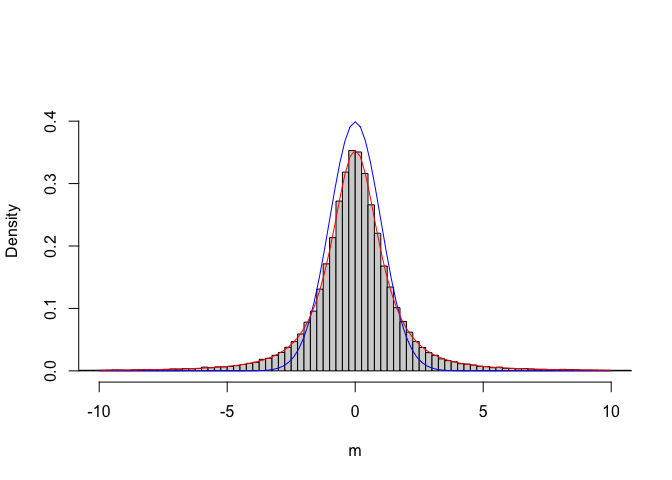
\includegraphics[width=0.85\linewidth]{_main_files/figure-latex/figName71-1} 

}

\caption{Sampling distribution empirica a confronto con una distribuzione normale (in rosso) e una distribuzione t di Student con due gradi di libertà}\label{fig:figName71}
\end{figure}

Senza ricorrere alla simulazione Monte Carlo, possiamo quindi risolvere il problema utilizzando la distribuzione t di Student, nella quale cercheremo la probabilità di ottenere valori di T minori o uguali a quello da noi osservato:

\begin{Shaded}
\begin{Highlighting}[]
\KeywordTok{pt}\NormalTok{(Ti, }\DataTypeTok{df=}\DecValTok{2}\NormalTok{)}
\CommentTok{## [1] 0.005067503}
\end{Highlighting}
\end{Shaded}

dove gli argomenti indicano rispettivamente il valore osservato. Il P-level è molto simile a quello ottenuto con la simulazione Monte Carlo.

Allo stesso valore, più semplicemente, si giunge utilizzando la funzione ``t.test()'':

\begin{Shaded}
\begin{Highlighting}[]
\KeywordTok{t.test}\NormalTok{(Y, }\DataTypeTok{mu=}\DecValTok{200}\NormalTok{, }\DataTypeTok{alternative=}\StringTok{"less"}\NormalTok{)}
\CommentTok{## }
\CommentTok{##  One Sample t-test}
\CommentTok{## }
\CommentTok{## data:  Y}
\CommentTok{## t = -9.8575, df = 2, p-value = 0.005068}
\CommentTok{## alternative hypothesis: true mean is less than 200}
\CommentTok{## 95 percent confidence interval:}
\CommentTok{##      -Inf 144.1333}
\CommentTok{## sample estimates:}
\CommentTok{## mean of x }
\CommentTok{##  120.6192}
\end{Highlighting}
\end{Shaded}

\hypertarget{interpretazione-del-p-level}{%
\subsection{Interpretazione del P-level}\label{interpretazione-del-p-level}}

Quando il P-level è inferiore a 0.05, concludiamo che vi sono prove scientifiche sufficientemente forti per rifiutare la nostra ipotesi di partenza.

Bisogna sottolineare come il P-level nella statistica tradizionale sia stato inizialmente proposto da Fisher come criterio di comportamento e non come un vero e proprio criterio inferenziale-probabilistico. Successivamente, Jarzy Neyman ed Egon Pearson, intorno al 1930, proposero di utilizzare il P-level come probabilità di errore di I specie, cioè come probabilità di rifiutare erroneamente l'ipotesi nulla. Tuttavia, trattandosi di una probabilità calcolata a partire da una \emph{sampling distribution}, cioè da un'ipotetica infinita ripetizione dell'esperimento, essa non ha alcun valore in relazione al singolo esperimento effettivamente eseguito, come i due autori menzionati in precedenza hanno esplicitamente chiarito.

Di conseguenza, nel caso in esempio, affermare che abbiamo una probabilità di errore pari a 0.0051 nel rifiutare l'ipotesi nulla, rappresenterebbe un abuso: le nostre conclusioni potrebbero essere false o vere, ma non abbiamo alcun elemento per scegliere tra le due opzioni. Possiamo solo affermare che, se ripetessimo infinite volte l'esperimento e se l'ipotesi nulla fosse vera, otterremmo un risultato estremo come il nostro o più estremo solo in 5 casi (circa) su 1000. In altre parole, nel lungo periodo, basando le nostre conclusioni sul criterio anzidetto (rifiuto l'ipotesi nulla se il P-value è inferiore a 0.05) commettiamo un errore in non più del 5\% dei casi. Insomma, il P-level non può essere guardato come la probabilità di `falso-positivo' ad ogni singolo test, ma solo nel lunghissimo periodo.

\hypertarget{confronto-tra-due-medie-il-test-t-di-student}{%
\section{Confronto tra due medie: il test t di Student}\label{confronto-tra-due-medie-il-test-t-di-student}}

Un ricercatore ha scelto casualmente dieci piante da una popolazione; ne ha trattate cinque con l'erbicida A e cinque con il placebo P. Alla fine dell'esperimento ha determinato il peso di ognuna delle dieci piante. E' evidente che le piante in prova sono solo un campione di quelle possibili, così come è evidente che il peso, come ogni altra variabile biologica, è soggetto ad una certa variabilità naturale, legata sia a questioni genotipiche che fenotipiche, oltre che ad eventuali errori casuali di misura.

I risultati sono i seguenti:

\begin{Shaded}
\begin{Highlighting}[]
\NormalTok{A <-}\StringTok{ }\KeywordTok{c}\NormalTok{(}\DecValTok{65}\NormalTok{, }\DecValTok{68}\NormalTok{, }\DecValTok{69}\NormalTok{, }\DecValTok{71}\NormalTok{, }\DecValTok{78}\NormalTok{)}
\NormalTok{P <-}\StringTok{ }\KeywordTok{c}\NormalTok{(}\DecValTok{80}\NormalTok{, }\DecValTok{81}\NormalTok{, }\DecValTok{84}\NormalTok{, }\DecValTok{88}\NormalTok{, }\DecValTok{94}\NormalTok{)}
\end{Highlighting}
\end{Shaded}

Nel campione A la media è pari a 70.2, mentre la deviazione standard è pari a 4.87. L'errore standard è pari a 2.18 e quindi l'intervallo di confidenza della media è 70.2 \(\pm\) 6.04. Invece, nel campione P, la media è 85.4, mentre la deviazione standard è pari a 5.72. L'errore standard è pari a 2.56, mentre l'intervallo di confidenza per la media è 85.4 \(\pm\) 7.11

Possiamo affermare che l'erbicida A riduce il peso delle piante trattate, coerentemente con le aspettative riguardo ad una molecola di questo tipo? Nel rispondere a questa domanda bisogna tener presente che i campioni sono totalmente irrilevanti, dato che il nostro interesse è rivolto alle popolazioni che hanno generato i campioni. Vogliamo cioè che le nostre conclusioni abbiano carattere di universalità e non siano specifiche a quanto abbiamo osservato nel nostro esperimento. Intanto possiamo notare che il limite di confidenza superiore per A (70.2 + 6.04 = 76.24) è inferiore al limite di confidenza inferiore per P (75.4 - 7.11 = 68.29). Questo non è un criterio sul quale basare le nostre considerazioni, ma è comunque un segno che le popolazioni da cui provengono i due campioni potrebbero essere diverse.

Per trovare un criterio decisionali più rigoroso, possiamo formulare \textbf{l'ipotesi nulla in questi termini}:

\[H_0: \mu_1 = \mu_2 = \mu\]

In altre parole, la nostra ipotesi di lavoro è che i due campioni siano in realtà estratti da due distribuzioni normali con la stessa media e la stessa deviazione standard, il che equivale a dire che essi provengono da un'unica distribuzione normale con media \(\mu\) e deviazione standard \(\sigma\).

L'ipotesi alternativa semplice può essere definita:

\[H_1 :\mu_1  \ne \mu_2\]

Se avessimo elementi sufficienti già prima di effettuare l'esperimento (e non dopo aver visto i risultati), potremmo anche adottare ipotesi alternative complesse, del tipo

\[H_1 :\mu _1  > \mu _2\]

oppure:

\[H_1 :\mu _1  < \mu _2\]

Quale statistica potrebbe meglio descrivere l'andamento dell'esperimento, in relazione all'ipotesi nulla? E' evidente che questa statistica dovrebbe essere basata su due indicatori diversi:

\begin{enumerate}
\def\labelenumi{\arabic{enumi}.}
\tightlist
\item
  l'entità della differenza tra le medie: più la differenza tra le due medie è alta e più è probabile che essa sia significativa;
\item
  l'entità dell'errore standard. Più è elevata la variabilità dei dati (e quindi l'errore di stima) più è bassa la probabilità che le differenze osservate tra le medie siano significative.
\end{enumerate}

Su queste basi, si può individuare la seguente statistica:

\[T = \frac{m_1 - m_2}{SED}\]

Si può osservare che T, in realtà, non è altro che il rapporto tra le quantità indicate in precedenza ai punti 1 e 2: infatti la quantità al numeratore è la differenza tra le medie dei due campioni, mentre la quantità al denominatore è il cosiddetto errore standard della differenza tra due medie (SED). Quest'ultima quantità si può ottenere pensando che i due campioni sono estratti in modo indipendente e, pertanto, la varianza della somma (algebrica) è uguale alla somma delle varianze. La varianza delle due medie è data dal quadrato delle loro deviazioni standard, cioè dal quadrato degli errori standard (SEM). Pertanto:

\[SED^2 = SEM_1^2 + SEM_2^2\]

Sappiamo anche che il SEM si ottiene dividendo la deviazione standard di ogni campione per la radice quadrata del numero dei dati, quindi:

\[SED^2 = \frac{s_1^2}{n_1} +  \frac{s_2^2}{n_2}\]

cioè:

\[SED = \sqrt{ \frac{s_1^2}{n_1} +  \frac{s_2^2}{n_2} }\]

Possiamo anche scrivere:

\[SED = \sqrt{ \frac{s_1^2 \, n_2 + s_2^2 \, n_1}{n_1 \, n_2} }\]

e, se le varianze sono uguali (\(s_1^2 = s_2^2 = s^2\)), segue che:

\[SED = \sqrt {s^2 \frac{n_1  + n_2}{n_1 \, n_2 } }\]

Se fosse anche \(n_1 = n_2 =n\), potremmo scrivere:

\[SED = \sqrt{2 \, \frac{s^2}{n} } = \sqrt{2} \times SEM\]

Il valore osservato per T è quindi uguale a:

\[T = \frac{85.4 - 70.2}{3.361547} = 4.5217\]

dove il denominatore è ottenuto come:

\[SED = \sqrt{ 2.18^2 +  2.56^2 } = 3.361547\]

A questo punto avendo osservato T = 4.5217, possiamo chiederci: qual è la `sampling distribution' per T, cioè quali valori potrebbe assumere questa statistica se ripetessimo il campionamento infinite volte, assumendo che l'ipotesi nulla fosse vera?

La sampling distribution per T potrebbe essere ottenuta empiricamente, utilizzando una simulazione Monte Carlo. Il codice da utilizzare per questa simulazione è fornito in appendice, dove si può vedere che, formalmente, la sampling distribution per T è una distribuzione t di Student, con 8 gradi di libertà (quattro per campione). Siamo quindi in grado di calcolare la probabilità di ottenere valori di T altrettanto estremi o più estremi di quello da noi osservato, tenendo però presente che il test è `a due code'. Infatti, il T osservato è positivo, ma solo perché abbiamo scritto la differenza come \(m_2 - m_1\) invece che come \(m_1 - m_2\). Tuttavia, entrambe le differenze sono possibili, quindi dobbiamo considerare anche il valore reciproco -T. In altre parole, ci chiediamo qual è la possibilità di campionare da una distribuzione t di Student valori esterni all'intervallo (-4.5217; 4.5217). La risposta, con R, è piuttosto semplice da ottenere:

\begin{Shaded}
\begin{Highlighting}[]
\DecValTok{2} \OperatorTok{*}\StringTok{ }\KeywordTok{pt}\NormalTok{(}\OperatorTok{-}\FloatTok{4.5217}\NormalTok{, }\DecValTok{8}\NormalTok{, }\DataTypeTok{lower.tail=}\NormalTok{T)}
\CommentTok{## [1] 0.00194554}
\end{Highlighting}
\end{Shaded}

Abbiamo moltiplicato per 2 il risultato, in quanto la funzione `dt()' fornisce la probabilità di trovare individui inferiori a -4.5217 (`lower.tail = T'). Essendo la distribuzione simmetrica, la probabilità di trovare soggetti superiori a 4.5217 è esattamente la stessa.

Vediamo che il P-level è minore di 0.05 e possiamo quindi rifiutare l'ipotesi nulla. Concludiamo che vi è un'evidenza scientifica abbastanza forte per ritenere che l'erbicida A induca una riduzione del peso delle piante trattate.

Allo stesso valore, più semplicemente, si perviene utilizzando la funzione:

\begin{Shaded}
\begin{Highlighting}[]
\KeywordTok{t.test}\NormalTok{(A, P, }\DataTypeTok{var.equal=}\NormalTok{T)}
\CommentTok{## }
\CommentTok{##  Two Sample t-test}
\CommentTok{## }
\CommentTok{## data:  A and P}
\CommentTok{## t = -4.5217, df = 8, p-value = 0.001945}
\CommentTok{## alternative hypothesis: true difference in means is not equal to 0}
\CommentTok{## 95 percent confidence interval:}
\CommentTok{##  -22.951742  -7.448258}
\CommentTok{## sample estimates:}
\CommentTok{## mean of x mean of y }
\CommentTok{##      70.2      85.4}
\end{Highlighting}
\end{Shaded}

Gli argomenti della funzione `t.test()' sono i due vettori è l'argomento `var.equal', che in questo caso è stato settato su TRUE. Chi volesse comprendere meglio il motivo di questa specifica, può leggerlo in appendice, alla fine del capitolo. Per gli altri, precisiamo solo che il test di t così eseguito è valido quando i due campioni sono indipendenti ed estratti da distribuzioni gaussiane con la stessa varianza. Queste assunzioni, soprattutto la seconda, sono sostenibili solo se le varianze osservate per i due campioni sono molto simili, con una differenza al di sotto di un ordine di grandezza, come accade nel nostro esempio.

\hypertarget{confronto-tra-due-proporzioni-il-test-chi2}{%
\section{\texorpdfstring{Confronto tra due proporzioni: il test \(\chi^2\)}{Confronto tra due proporzioni: il test \textbackslash{}chi\^{}2}}\label{confronto-tra-due-proporzioni-il-test-chi2}}

Il test di t è molto utile, ma soltanto nel caso in cui si abbia a che fare con caratteri quantitativi, cioè con variabili misurate su una scala continua, per le quali sia possibile calcolare statistiche descrittive, come appunto la media. Talvolta, i ricercatori sono interessati a rilevare caratteristiche qualitative, come ad esempio lo stato di una pianta in seguito ad un trattamento (morta o viva), il colore dei semi (si ricordino i piselli verdi e gialli di Mendel) ed altre caratteristiche che non sono misurabili su una scala continua.

Avendo a che fare con variabili qualitative, l'unica statistica rilevabile è il numero di soggetti che presentano le diverse modalità. Ad esempio, immaginiamo un esperimento per verificare se un coadiuvante aumenta l'efficacia di un insetticida. In questo esperimento, utilizziamo l'insetticida da solo e miscelato con il coadiuvante su due gruppi di insetti diversi. Nel primo gruppo (trattato con insetticida) contiamo 56 morti su 75 insetti trattate, mentre nel secondo gruppo (trattato con insetticida e coadiuvante) otteniamo 48 morti su 50 insetti trattati.

I risultati di questo esperimento si riducono ad una tabella di contingenza:\footnote{da Wikipedia: \emph{Le tabelle di contingenza sono un particolare tipo di tabelle a doppia entrata (cioè tabelle con etichette di riga e di colonna), utilizzate in statistica per rappresentare e analizzare le relazioni tra due o più variabili. In esse si riportano le frequenze congiunte delle variabili}}

\begin{Shaded}
\begin{Highlighting}[]
\NormalTok{counts <-}\StringTok{ }\KeywordTok{c}\NormalTok{(}\DecValTok{56}\NormalTok{, }\DecValTok{19}\NormalTok{, }\DecValTok{48}\NormalTok{, }\DecValTok{2}\NormalTok{)}
\NormalTok{tab <-}\StringTok{ }\KeywordTok{matrix}\NormalTok{(counts, }\DecValTok{2}\NormalTok{, }\DecValTok{2}\NormalTok{, }\DataTypeTok{byrow =}\NormalTok{ T)}
\KeywordTok{row.names}\NormalTok{(tab) <-}\StringTok{ }\KeywordTok{c}\NormalTok{(}\StringTok{"I"}\NormalTok{, }\StringTok{"IC"}\NormalTok{)}
\KeywordTok{colnames}\NormalTok{(tab) <-}\StringTok{ }\KeywordTok{c}\NormalTok{(}\StringTok{"M"}\NormalTok{, }\StringTok{"V"}\NormalTok{)}
\NormalTok{tab}
\CommentTok{##     M  V}
\CommentTok{## I  56 19}
\CommentTok{## IC 48  2}
\end{Highlighting}
\end{Shaded}

Per una tabella di contingenza, possiamo determinare una statistica che misura la connessione tra variabili (trattamento e mortalità), detta \(\chi^2\). La connessione è l'indicatore giusto per rispondere alla nostra domanda di ricerca; infatti ci stiamo chiedendo se la proporzione dei morti è indipendente dal tipo di trattamento oppure no.

Con R, il \(\chi^2\) si calcola applicando la funzione summary all'oggetto `data.table'. Dato che la nostra tabella `tab' è, in realtà, una matrice (almeno così come l'abbiamo creata), prima di interrogarla con il metodo `summary()' dobbiamo trasformarla in un oggetto `data.table', con la funzione `as.table()':

\begin{Shaded}
\begin{Highlighting}[]
\KeywordTok{summary}\NormalTok{( }\KeywordTok{as.table}\NormalTok{(tab) )}
\CommentTok{## Number of cases in table: 125 }
\CommentTok{## Number of factors: 2 }
\CommentTok{## Test for independence of all factors:}
\CommentTok{##  Chisq = 9.768, df = 1, p-value = 0.001776}
\end{Highlighting}
\end{Shaded}

Il valore di \(\chi^2\) osservato è pari a 9.768, il che indica un certo grado di connessione. Infatti, ricordiamo che, in caso di indipendenza tra le variabili, \(\chi^2\) dovrebbe essere zero. Tuttavia, noi non siamo interessati ai due campioni, in quanto i 125 soggetti osservati sono tratti da due popolazioni più ampie. Considerando queste due popolazioni, poniamo l'ipotesi nulla in questi termini:

\[H_o :\pi_1  = \pi_2  = \pi\]

Vediamo che, come negli altri esempio, l'ipotesi nulla riguarda i parametri delle popolazioni (\(\pi_1\) e \(\pi_2\)), non quelli dei campioni (\(p_1\) e \(p_2\)). Ci chiediamo: se l'ipotesi nulla è vera (\(\pi_1 = \pi_2\)), qual è la sampling distribution per \(\chi^2\)? E soprattutto, quanto è probabile ottenere un valore alto come il nostro o più alto?

In appendice mostriamo come si possa arrivare a questo risultato con una simulazione Monte Carlo. In modo formale, si può dimostrare che, se \(n\) è sufficientemente grande (n \textgreater{} 30), il valore osservato di \(\chi^2\) segue appunto la distribuzione di probabilità \(\chi^2\), con un numero di gradi di libertà \(\nu\) pari al numero dei dati indipendenti, che, in questo caso, è pari ad 1. Infatti, una volta fissata una frequenza, le altre sono automaticamente definite, dovendo restituire i totali marginali. In R, possiamo utilizzare la funzione `pchi()' per calcolare la probabilità di ottenere valori pari o superiori a 9.768:

\begin{Shaded}
\begin{Highlighting}[]
\KeywordTok{pchisq}\NormalTok{(}\FloatTok{9.76801}\NormalTok{, }\DecValTok{1}\NormalTok{, }\DataTypeTok{lower.tail=}\NormalTok{F)}
\CommentTok{## [1] 0.001775746}
\end{Highlighting}
\end{Shaded}

Allo stesso risultato, ma in modo più semplice, è possibile pervenire utilizzando la già citata funzione `summary()', applicata alla tabella di contingenza (vedi sopra), oppure:

\begin{Shaded}
\begin{Highlighting}[]
\KeywordTok{chisq.test}\NormalTok{(tab, }\DataTypeTok{correct =}\NormalTok{ F)}
\CommentTok{## }
\CommentTok{##  Pearson's Chi-squared test}
\CommentTok{## }
\CommentTok{## data:  tab}
\CommentTok{## X-squared = 9.768, df = 1, p-value = 0.001776}
\end{Highlighting}
\end{Shaded}

Come nel caso del `t' di Student, abbiamo diversi tipi di test di chi quadro. In particolare, possiamo applicare o no la correzione per la continuità, che è necessaria quando il numero dei soggetti è piccolo (minore di 30, grosso modo),. Nel nostro caso, non lo abbiamo ritenuto necessario ed abbiamo quindi aggiunto l'argomento `correct = F'.

\hypertarget{conclusioni-1}{%
\section{Conclusioni}\label{conclusioni-1}}

Abbiamo visto quale strumento abbiamo a disposizione per tirare conclusioni in presenza di incertezza sperimentale. Dovrebbe essere evidente che anche le nostre conclusioni sono incerte, in quanto soggette all'errore di campionamento. In particolare, abbiamo visto che esiste un rischio di errore di prima specie, cioè rifiutare erronamente l'ipotesi nulla (falso positivo). Allo stesso modo, esiste anche un rischio di errore di II specie, cioè accettare erroneamente l'ipotesi nulla (falso negativo). Di questi due tipi di errore abbiamo parlato più diffusamente in appendice.

\hypertarget{riepilogo}{%
\section{Riepilogo}\label{riepilogo}}

Lo schema di lavoro, nel test d'ipotesi, è il seguente:

\begin{enumerate}
\def\labelenumi{\arabic{enumi}.}
\tightlist
\item
  Si formula l'ipotesi nulla;
\item
  Si individua una statistica che descriva l'andamento dell'esperimento, in relazione all'ipotesi nulla;
\item
  Si individua la sampling distribution per questa statistica, assumendo vera l'ipotesi nulla; la sampling distribution può essere empirica (ottenuta per simulazione) o teorica, scelta in base a considerazioni probabilistiche
\item
  Si calcola la probabilità che, essendo vera l'ipotesi nulla, si possa osservare una valore altrettanto estremo o più estremo di quello calcolato, per la statistica di riferimento;
\item
  Se il livello di probabilità è inferiore ad una certa soglia \(\alpha\) prefissata (generalmente 0.05), si rifiuta l'ipotesi nulla.
\end{enumerate}

\hypertarget{esercizi-1}{%
\section{Esercizi}\label{esercizi-1}}

\begin{enumerate}
\def\labelenumi{\arabic{enumi}.}
\tightlist
\item
  Uno sperimentatore ha impostato un esperimento verificare l'effetto di un fungicida (A) in confronto al testimone non trattato (B), in base al numero di colonie fungine sopravvissute. Il numero delle colonie trattate è di 200, con 180 colonie sopravvissute al trattamento. Il numero di quelle non trattate è di 100, con 50 colonie sopravvissute. Stabilire se i risultati possono essere considerati significativamente diversi, per un livello di probabilità del 5\%
\item
  Uno sperimentatore ha impostato un esperimento per confrontare due tesi sperimentali (A, B). Per la tesi A sono stati osservate le seguenti produzioni: 9.3, 10.2, 9.7. Per la tesi B, sono state osservati valori di 12.6, 12.3 e 12.5. Stabilire se i risultati possono essere considerati significativamente diversi, per un livello di probabilità del 5\%.
\item
  Uno sperimentatore ha impostato un esperimento per confrontare se l'effetto di un fungicida è significativo, in un disegno sperimentale con tre ripetizioni. Con il trattamento, i risultati produttivi (in t/ha) sono 65, 71 e 68. Con il non trattato, i risultati sono 54, 51 e 59. E'significativo l'effetto del trattamento fungicida sulla produzione, per un livello di probabilità di errore del 5\%?
\item
  Immaginate di aver riscontrato che, in determinate condizioni ambientali, 60 olive su 75 sono attaccate da \emph{Daucus olee} (mosca dell'olivo). Nelle stesse condizioni ambientali, diffondendo in campo un insetto predatore siamo riusciti a ridurre il numero di olive attaccate a 12 su 75. Si tratta di una oscillazione casuale del livello di attacco o possiamo concludere che l'insetto predatore è stato un mezzo efficace di lotta biologica alla mosca dell'olivo?
\end{enumerate}

\begin{center}\rule{0.5\linewidth}{\linethickness}\end{center}

\hypertarget{per-approfondire-un-po-4}{%
\section{Per approfondire un po'\ldots{}}\label{per-approfondire-un-po-4}}

\hypertarget{tipologie-alternative-di-test-t-di-student}{%
\subsection{Tipologie alternative di test t di Student}\label{tipologie-alternative-di-test-t-di-student}}

Chiunque abbia utilizzato un computer per eseguire un test di t, si sarà accorto che è necessario scegliere tra tre procedure alternative. Infatti, abbiamo:

\begin{enumerate}
\def\labelenumi{\arabic{enumi}.}
\tightlist
\item
  t-test appaiato. In questo caso le misure sono prese a coppia sullo stesso soggetto e non sono quindi indipendenti.
\item
  t-test omoscedastico. Le misure sono prese su soggetti diversi (indipendenti) e possiamo suppore che i due campioni provengano da due popolazioni con la stessa varianza.
\item
  t-test eteroscedastico. Le misure sono prese su soggetti diversi, ma le varianze non sono omogenee.
\end{enumerate}

Consideriamo i due campioni:

\begin{Shaded}
\begin{Highlighting}[]
\NormalTok{C1}
\CommentTok{## [1] 12.660770  9.947017 10.500794 13.471233 13.459139}
\NormalTok{C2}
\CommentTok{## [1] 16.14014 16.20918 12.96391 15.51307 14.91213}
\KeywordTok{mean}\NormalTok{(C1)}
\CommentTok{## [1] 12.00779}
\KeywordTok{mean}\NormalTok{(C2)}
\CommentTok{## [1] 15.14769}
\KeywordTok{var}\NormalTok{(C1)}
\CommentTok{## [1] 2.798071}
\KeywordTok{var}\NormalTok{(C2)}
\CommentTok{## [1] 1.767402}
\end{Highlighting}
\end{Shaded}

Vediamo che le medie sono diverse ma le varianze sono simili, dello stesso ordine di grandezza. Pertanto, possiamo utilizzare un test t omoscedastico, che garantisce un più alto livello di potenza.

\begin{Shaded}
\begin{Highlighting}[]
\KeywordTok{t.test}\NormalTok{(C1, C2, }\DataTypeTok{var.equal =}\NormalTok{ T, }\DataTypeTok{paired =}\NormalTok{ F)}
\CommentTok{## }
\CommentTok{##  Two Sample t-test}
\CommentTok{## }
\CommentTok{## data:  C1 and C2}
\CommentTok{## t = -3.2859, df = 8, p-value = 0.01109}
\CommentTok{## alternative hypothesis: true difference in means is not equal to 0}
\CommentTok{## 95 percent confidence interval:}
\CommentTok{##  -5.3434208 -0.9363712}
\CommentTok{## sample estimates:}
\CommentTok{## mean of x mean of y }
\CommentTok{##  12.00779  15.14769}
\end{Highlighting}
\end{Shaded}

Consideriamo invece quest'altra coppia di campioni:

\begin{Shaded}
\begin{Highlighting}[]
\NormalTok{D1}
\CommentTok{## [1] 12.06608 11.79470 11.85008 12.14712 12.14591}
\NormalTok{D2}
\CommentTok{## [1] 35.14014 35.20918 31.96391 34.51307 33.91213}
\KeywordTok{mean}\NormalTok{(D1)}
\CommentTok{## [1] 12.00078}
\KeywordTok{mean}\NormalTok{(D2)}
\CommentTok{## [1] 34.14769}
\KeywordTok{var}\NormalTok{(D1)}
\CommentTok{## [1] 0.02798071}
\KeywordTok{var}\NormalTok{(D2)}
\CommentTok{## [1] 1.767402}
\end{Highlighting}
\end{Shaded}

In questo caso le varianza sono molto diverse e l'assunzione di omoscedasticità non è tenibile. Dobbiamo utilizzare un test eteroscedastico e, di conseguenza, mentre il SED si calcola con la formula esposta più sopra, si pone il problema di stabilire il numero di gradi di libertà del SED stesso. Dato che il sed è ottenuto come somma di varianze, il numero di gradi di libertà può essere approssimato con la formula di Satterthwaite:

\[DF_s \simeq \frac{ \left( s^2_1 + s^2_2 \right)^2 }{ \frac{(s^2_1)^2}{DF_1} + \frac{(s^2_2)^2}{DF_2} }\]

Vediamo che se le varianze e i gradi di libertà sono uguali, la formula precedente riduce a:

\[DF_s = 2 \times DF\]

Nel nostro caso:

\begin{Shaded}
\begin{Highlighting}[]
\NormalTok{dfS <-}\StringTok{ }\NormalTok{(}\KeywordTok{var}\NormalTok{(D1) }\OperatorTok{+}\StringTok{ }\KeywordTok{var}\NormalTok{(D2))}\OperatorTok{^}\DecValTok{2} \OperatorTok{/}\StringTok{ }
\StringTok{  }\NormalTok{((}\KeywordTok{var}\NormalTok{(D1)}\OperatorTok{^}\DecValTok{2}\NormalTok{)}\OperatorTok{/}\DecValTok{4} \OperatorTok{+}\StringTok{ }\NormalTok{(}\KeywordTok{var}\NormalTok{(D2)}\OperatorTok{^}\DecValTok{2}\NormalTok{)}\OperatorTok{/}\DecValTok{4}\NormalTok{)}
\NormalTok{dfS}
\CommentTok{## [1] 4.126621}
\end{Highlighting}
\end{Shaded}

In effetti:

\begin{Shaded}
\begin{Highlighting}[]
\KeywordTok{t.test}\NormalTok{(D1, D2, }\DataTypeTok{var.equal=}\NormalTok{F)}
\CommentTok{## }
\CommentTok{##  Welch Two Sample t-test}
\CommentTok{## }
\CommentTok{## data:  D1 and D2}
\CommentTok{## t = -36.959, df = 4.1266, p-value = 2.326e-06}
\CommentTok{## alternative hypothesis: true difference in means is not equal to 0}
\CommentTok{## 95 percent confidence interval:}
\CommentTok{##  -23.79070 -20.50312}
\CommentTok{## sample estimates:}
\CommentTok{## mean of x mean of y }
\CommentTok{##  12.00078  34.14769}
\end{Highlighting}
\end{Shaded}

Se le misure in D1 e D2 fossero state rilevate sugli stessi soggetti (due misure per soggetto), allora avremmo cinque soggetti invece che dieci e, di conseguenza solo 4 gradi di libertà:

\begin{Shaded}
\begin{Highlighting}[]
\KeywordTok{t.test}\NormalTok{(D1, D2, }\DataTypeTok{var.equal=}\NormalTok{F, }\DataTypeTok{paired=}\NormalTok{T)}
\CommentTok{## }
\CommentTok{##  Paired t-test}
\CommentTok{## }
\CommentTok{## data:  D1 and D2}
\CommentTok{## t = -38.002, df = 4, p-value = 2.864e-06}
\CommentTok{## alternative hypothesis: true difference in means is not equal to 0}
\CommentTok{## 95 percent confidence interval:}
\CommentTok{##  -23.76497 -20.52885}
\CommentTok{## sample estimates:}
\CommentTok{## mean of the differences }
\CommentTok{##               -22.14691}
\end{Highlighting}
\end{Shaded}

\hypertarget{simulazione-del-p-value-nel-test-dipotesi}{%
\subsection{Simulazione del P-value nel test d'ipotesi}\label{simulazione-del-p-value-nel-test-dipotesi}}

Più sopra abbiamo visto che il test d'ipotesi viene eseguito sulla base del principio che, quando l'ipotesi nulla è vera, una statistica campionaria (T, \(\chi^2\) o altro) mostra una certa variabilità tra un campionamento e l'altro. Quando i campionamenti sono tanti (meglio, infiniti), i valori ottenuti danno origine ad una \emph{sampling distribution}, che può essere modellizzata utilizzando una qualche distribuzione di probabilità formale, come il t di Student il chi quadro e così via.

Invece che ricorrere ad una distribuzione di probabilità nota, possiamo costruire una sampling distribution empirica, utilizzando le simulazioni Monte Carlo. In questo caso, il campionamento viene ripetuto molte volte, assumendo che l'ipotesi nulla sia vera. Mostriamo ora come questo approccio possa essere utilizzato per confrontare due medie oppure due proporzioni campionarie.

Immaginiamo di avere i due campioni, A e P, indicati in precedenza, con un T osservato pari a -4.521727. Se i due campioni fossero estratti dalla stessa popolazione normale, questa dovrebbe avere una media pari a (70.2 + 85.4)/2 = 77.8 e una deviazione standard pari alla deviazione standard delle dieci osservazioni (tutte insieme, senza distinzioni di trattamento), cioè 9.45.

\begin{Shaded}
\begin{Highlighting}[]
\NormalTok{media <-}\StringTok{ }\KeywordTok{mean}\NormalTok{(}\KeywordTok{c}\NormalTok{(A, P))}
\NormalTok{devSt <-}\StringTok{ }\KeywordTok{sd}\NormalTok{(}\KeywordTok{c}\NormalTok{(A, P))}
\NormalTok{media}
\CommentTok{## [1] 77.8}
\NormalTok{devSt}
\CommentTok{## [1] 9.44928}
\end{Highlighting}
\end{Shaded}

Proviamo ora ad utilizzare un generatore di numeri casuali gaussiani per estrarre numerose (100'000) coppie di campioni, e calcolare, per ogni coppia, il valore T, come abbiamo fatto con la nostra coppia iniziale.

Il codice da utilizzare in R per le simulazioni è il seguente:

\begin{Shaded}
\begin{Highlighting}[]
\NormalTok{T_obs <-}\StringTok{ }\FloatTok{-4.521727}
\KeywordTok{set.seed}\NormalTok{(}\DecValTok{34}\NormalTok{)}
\NormalTok{result <-}\StringTok{ }\KeywordTok{rep}\NormalTok{(}\DecValTok{0}\NormalTok{, }\DecValTok{100000}\NormalTok{)}
\ControlFlowTok{for}\NormalTok{ (i }\ControlFlowTok{in} \DecValTok{1}\OperatorTok{:}\DecValTok{100000}\NormalTok{)\{}
\NormalTok{  sample1 <-}\StringTok{ }\KeywordTok{rnorm}\NormalTok{(}\DecValTok{5}\NormalTok{, media, devSt)}
\NormalTok{  sample2 <-}\StringTok{ }\KeywordTok{rnorm}\NormalTok{(}\DecValTok{5}\NormalTok{, media, devSt)}
\NormalTok{  SED <-}\StringTok{ }\KeywordTok{sqrt}\NormalTok{( (}\KeywordTok{sd}\NormalTok{(sample1)}\OperatorTok{/}\KeywordTok{sqrt}\NormalTok{(}\DecValTok{5}\NormalTok{))}\OperatorTok{^}\DecValTok{2} \OperatorTok{+}
\StringTok{                 }\NormalTok{(}\KeywordTok{sd}\NormalTok{(sample2)}\OperatorTok{/}\KeywordTok{sqrt}\NormalTok{(}\DecValTok{5}\NormalTok{))}\OperatorTok{^}\DecValTok{2}\NormalTok{ )}
\NormalTok{  result[i] <-}\StringTok{ }\NormalTok{(}\KeywordTok{mean}\NormalTok{(sample1) }\OperatorTok{-}\StringTok{ }\KeywordTok{mean}\NormalTok{(sample2)) }\OperatorTok{/}\StringTok{ }\NormalTok{SED}
\NormalTok{\}}

\KeywordTok{length}\NormalTok{(result[result }\OperatorTok{<}\StringTok{ }\NormalTok{T_obs]) }\OperatorTok{/}\StringTok{ }\DecValTok{100000}
\CommentTok{## [1] 0.00095}
\KeywordTok{length}\NormalTok{(result[result }\OperatorTok{>}\StringTok{ }\OperatorTok{-}\StringTok{ }\NormalTok{T_obs]) }\OperatorTok{/}\DecValTok{100000}
\CommentTok{## [1] 0.00082}
\end{Highlighting}
\end{Shaded}

Possiamo notare che, dei 100'000 valori di T osservati assumendo vera l'ipotesi nulla, meno dell'un per mille sono inferiori a quello da noi osservato e altrettanti sono superiori al suo reciproco (4.5217). In totale, la probabilità di osservare un valore di T così alto in valore assoluto e dello 0.18 \%, molto simile a quella ottenuta più sopra con il test t di Student.

E se dobbiamo confrontare due proporzioni? Prendiamo la tabella di contingenze utilizzata più sopra:

\begin{Shaded}
\begin{Highlighting}[]
\NormalTok{tab}
\CommentTok{##     M  V}
\CommentTok{## I  56 19}
\CommentTok{## IC 48  2}
\end{Highlighting}
\end{Shaded}

La connessione si esprime con la statistica chi quadro e il valore osservato è 9.768. Qual è la probabilità che, se i caratteri sono indipendenti, si produca un valore di chi quadro pari o superiore a 9.768?

Per la simulazione possiamo utilizzare la funzione `r2dtable()', che produce il numero voluto di tabelle di contingenza, con righe e colonne indipendenti, rispettando i totali marginali voluti. Le tabelle prodotte (nel nostro caso 10'000) sono restituite come lista, quindi possiamo utilizzare la funzione `lapply()' per applicare ad ogni elemento della lista la funzione che restituisce il \(\chi^2\) (`chiSim').

\begin{Shaded}
\begin{Highlighting}[]
\NormalTok{chiSim <-}\StringTok{ }\ControlFlowTok{function}\NormalTok{(x) }\KeywordTok{summary}\NormalTok{(}\KeywordTok{as.table}\NormalTok{(x))}\OperatorTok{$}\NormalTok{stat}
\KeywordTok{set.seed}\NormalTok{(}\DecValTok{1234}\NormalTok{)}
\NormalTok{tabs <-}\StringTok{ }\KeywordTok{r2dtable}\NormalTok{(}\DecValTok{10000}\NormalTok{, }\KeywordTok{apply}\NormalTok{(tab, }\DecValTok{1}\NormalTok{, sum), }\KeywordTok{apply}\NormalTok{(tab, }\DecValTok{2}\NormalTok{, sum))}
\NormalTok{chiVals <-}\StringTok{ }\KeywordTok{as.numeric}\NormalTok{( }\KeywordTok{lapply}\NormalTok{( tabs, chiSim) )}
\KeywordTok{length}\NormalTok{(chiVals[chiVals }\OperatorTok{>}\StringTok{ }\FloatTok{9.768}\NormalTok{])}
\CommentTok{## [1] 19}
\end{Highlighting}
\end{Shaded}

Vediamo che vi sono 19 valori più alti di quello da noi osservato, quindi il p-value è 0.0019. Anche in questo caso molto simile a quello ottenuto con un test statistico formale.

\hypertarget{altre-letture-2}{%
\subsection{Altre letture}\label{altre-letture-2}}

\begin{enumerate}
\def\labelenumi{\arabic{enumi}.}
\tightlist
\item
  Hastie, T., Tibshirani, R., Friedman, J., 2009. The elements of statistical learning, Springer Series in Statistics. Springer Science + Business Media, California, USA.
\end{enumerate}

\hypertarget{modelli-anova-ad-una-via}{%
\chapter{Modelli ANOVA ad una via}\label{modelli-anova-ad-una-via}}

Nel capitolo 4 abbiamo già parlato di come assumiamo che risultati di un esperimento si generino attraverso un doppio meccanismo deterministico e stocastico, rappresentabile attraverso un modello matematico contenento uno o più elementi casuali, descritti da una funzione di densità, solitamente gaussiana. Abbiamo già visto che i modelli più utilizzati sono lineari e, tra questi, il gruppo più diffuso, almeno in ambito biologico-agrario, è quello dei modelli ANOVA.

La nomenclatura è impropria; infatti, con il termine ANOVA, si intende un'operazione di scomposizione della varianza, inventata da Fisher negli anni `30 del '900, che costituisce ancora oggi una delle più fondamentali tecniche di analisi dei dati sperimentali. Tuttavia, ci sono alcuni modelli che, più naturalmente di altri, sono connessi all'esecuzione dell'ANOVA fisheriana. Si tratta di modelli lineari nei quali la/le variabile/i indipendenti, che descrivono gli stimoli sperimentali, sono nominali (categoriche) e, nella letteratura anglosassone, prendono il nome di 'factors' (fattori sperimentali).

Questi modelli rappresentano il punto di ingresso nell'analisi dei dati e la gran parte della letteratura scientifica è basata proprio su questi modelli. Pertanto, ad essi dedicheremo ampio spazio nel seguito di questo libro.

\hypertarget{caso-studio-confronto-tra-erbicidi-in-vaso}{%
\section{Caso-studio: confronto tra erbicidi in vaso}\label{caso-studio-confronto-tra-erbicidi-in-vaso}}

Abbiamo eseguito un esperimento in vaso, nel quale abbiamo utilizzato quattro trattamenti erbicidi:

\begin{enumerate}
\def\labelenumi{\arabic{enumi}.}
\tightlist
\item
  Metribuzin
\item
  Rimsulfuron
\item
  Metribuzin + rimsulfuron
\item
  Testimone non trattato
\end{enumerate}

Lo scopo dell'esperimento era quello di verificare se la miscela metribuzin e rimsulfuron è più efficace dei due componenti utilizzati separatamente. L'esperimento era disegnato a randomizzazione completa con quattro repliche e prevedeva il rilievo della biomassa presente su ogni vaso, tre settimane dopo il trattamento: un più basso valore di biomassa implica un miglior effetto del trattamento.

I risultati di questo esperimento sono riportati nel dataset `mixture.csv', che è disponibile su gitHub. Per prima cosa, carichiamo il file.

\vspace{12pt}

\begin{Shaded}
\begin{Highlighting}[]
\NormalTok{str1 <-}\StringTok{ "https://raw.githubusercontent.com/OnofriAndreaPG"}
\NormalTok{str2 <-}\StringTok{ "/agroBioData/master/mixture.csv"}
\NormalTok{pathData <-}\StringTok{ }\KeywordTok{paste}\NormalTok{(str1, str2, }\DataTypeTok{sep =} \StringTok{""}\NormalTok{)}

\NormalTok{dataset <-}\StringTok{ }\KeywordTok{read.csv}\NormalTok{(pathData, }\DataTypeTok{header =}\NormalTok{ T)}
\KeywordTok{head}\NormalTok{(dataset)}
\CommentTok{##             Treat Weight}
\CommentTok{## 1        Unweeded  24.62}
\CommentTok{## 2        Unweeded  30.94}
\CommentTok{## 3        Unweeded  24.02}
\CommentTok{## 4        Unweeded  27.51}
\CommentTok{## 5 Metribuzin__348  15.20}
\CommentTok{## 6 Metribuzin__348   4.38}
\end{Highlighting}
\end{Shaded}

Il dataset è organizzato come un database, nel quale ogni riga contraddistingue un'unità sperimentale (record) e ogni colonna rappresenta una caratteristica del record (campo). In questo caso abbiamo due colonne: una per la variabile indipendente (fattore sperimentale `Treat'), che ci dice con quale erbicida è stata trattata ogni unità sperimentale, ed una per la variabile dipendente (`Weight').

\hypertarget{descrizione-del-dataset}{%
\section{Descrizione del dataset}\label{descrizione-del-dataset}}

La prima analisi dei dati consiste nella valutazione descrittiva del dataset. In particolare, calcoliamo:

\begin{enumerate}
\def\labelenumi{\arabic{enumi}.}
\tightlist
\item
  le medie per ogni tesi sperimentale
\item
  Le deviazioni standard per ogni tesi sperimentale
\end{enumerate}

Utilizziamo la funzione `tapply' in R.

\begin{Shaded}
\begin{Highlighting}[]
\NormalTok{medie <-}\StringTok{ }\KeywordTok{tapply}\NormalTok{(dataset}\OperatorTok{$}\NormalTok{Weight, dataset}\OperatorTok{$}\NormalTok{Treat, mean)}
\NormalTok{SDs <-}\StringTok{ }\KeywordTok{tapply}\NormalTok{(dataset}\OperatorTok{$}\NormalTok{Weight, dataset}\OperatorTok{$}\NormalTok{Treat, sd)}
\NormalTok{descrit <-}\StringTok{ }\KeywordTok{cbind}\NormalTok{(medie, SDs)}
\NormalTok{descrit}
\CommentTok{##                   medie      SDs}
\CommentTok{## Metribuzin__348  9.1750 4.699089}
\CommentTok{## Mixture_378      5.1275 2.288557}
\CommentTok{## Rimsulfuron_30  16.8600 4.902353}
\CommentTok{## Unweeded        26.7725 3.168673}
\end{Highlighting}
\end{Shaded}

Che cosa ci dice questa tabella, in base agli obiettivi dell'esperimento?

Ci suggerisce che:

\begin{enumerate}
\def\labelenumi{\arabic{enumi}.}
\tightlist
\item
  La miscela sembra leggermente più efficace dei prodotti singoli
\item
  Esiste una certa variabilità (errore sperimentale), che impedisce un giudizio certo
\item
  La variabilità è abbastanza simile per tutti i trattamenti
\end{enumerate}

\hypertarget{definizione-di-un-modello-lineare}{%
\section{Definizione di un modello lineare}\label{definizione-di-un-modello-lineare}}

Sappiamo che, dietro ai campioni osservati, vi sono una o più popolazioni di riferimento, alle quali è rivolto il nostro interesse: abbiamo infatti osservato \(m_1\), \(m_2\), \(m_3\) ed \(m_4\) (le medie dei campioni), ma siamo effettivamente interessati a conoscere \(\mu_1\), \(\mu_2\), \(\mu_3\) e \(\mu_4\), cioè le medie delle popolazioni da cui i campioni sono tratti. E siamo anche interessati a capire se la differenza è sufficientemente ampia da poter ritenere che non sia di natura puramente casuale.

Per descrivere le osservazioni possiamo utilizzare un modello lineare del tipo:

\[Y_i = \mu + \alpha_j + \varepsilon_i\]

Questo modello impone che le osservazioni \(Y\) derivino da una valore \(\mu\), detto intercetta, a cui si aggiunge l'effetto del trattamento \(\alpha_j\) e l'effetto stocastico \(\varepsilon\), che è un elemento che influenza ogni singola osservazione \(i\).

Il valore atteso per un soggetto, in assenza di errore sperimentale, è:

\[\bar{Y_i} = \mu + \alpha_j\]

È abbastanza facile intuire che, se non ci fosse l'errore sperimentale, un soggetto dovrebbe avere un valore pari alla media del gruppo di cui fa parte, per cui:

\[\bar{Y_i} = \mu_j = \mu + \alpha_j\]

\hypertarget{parametrizzazione-del-modello}{%
\section{Parametrizzazione del modello}\label{parametrizzazione-del-modello}}

Gli elementi \(\mu\) ed \(\alpha\) hanno un significato diverso a seconda della \textbf{parametrizzazione del modello}. Infatti, dobbiamo tener presente che, con il modello lineare sopra riportato, ci stiamo proponendo di ottenere la quantità \(Y_i\) come somma di tre valori ed, in questi termini, il problema è indeterminato. Infatti esistono infinite triplette di valori che, sommati, possono restituire \(Y_i\), qualunque esso sia. Per questo motivo dobbiamo porre un qualche vincolo su uno degli elementi in gioco. Esistono diversi tipi di vincoli, ma, in questo testo, ne tratteremo solo due, quelli più rilevanti.

\hypertarget{vincolo-sul-trattamento}{%
\subsection{Vincolo sul trattamento}\label{vincolo-sul-trattamento}}

Un vincolo molto usato è \(\alpha_1 = 0\). Di conseguenza, risulta che:

\[ \left\{ {\begin{array}{l}
\mu_1 = \mu + \alpha_1 = \mu + 0\\
\mu_2 = \mu + \alpha_2 \\
\mu_3 = \mu + \alpha_3 \\
\mu_4 = \mu + \alpha_4
\end{array}} \right.\]

quindi \(\mu\) è la media del primo trattamento, usualmente inteso in ordine alfabetico (ma il riferimento può cambiare, a seconda delle esigenze). Gli altri valori \(\alpha_j\), sono differenze tra le medie dei gruppi da 2 a 4 con la media del gruppo 1.

In generale, adottando il vincolo sul trattamento, i parametri sono medie, valori attesi oppure differenze tra medie e/o differenze tra valori attesi.

\hypertarget{vincolo-sulla-somma}{%
\subsection{Vincolo sulla somma}\label{vincolo-sulla-somma}}

Un altro possibile vincolo consiste nell'imporre che la somma degli \(\alpha_j\) sia pari a 0. In questo caso, abbiamo quattro gruppi, quindi quattro medie. Se prendiamo l'espressione precedente e sommiamo membro a membro, otteniamo:

\[ \mu_1 + \mu_2 + \mu_3 + \mu_4 = 4 \mu + \sum{\alpha_j}\]

Quindi, con il vincolo sulla somma:

\[ \mu_1 + \mu_2 + \mu_3 + \mu_4 = 4 \mu\]
Quindi:

\[\mu = \frac{\mu_1 + \mu_2 + \mu_3 + \mu_4}{4} \]

cioè \(\mu\) è la media generale e \(\alpha_j\) rappresentano gli scostamenti di ogni trattamento rispetto alla media generale, usualmente definiti \textbf{effetti dei trattamenti}. Se un prodotto è efficace, abbasserà di più il peso delle infestanti e quindi avrà un elevato effetto negativo.

La seconda parametrizzazione è forse più `comprensibile' e, se il disegno è bilanciato, è abbastanza facile stimare i parametri `a mano', utilizzando il metodo dei momenti, a partire dalle medie aritmetiche dei trattamenti.

I software statistici, invece, non utilizzano il metodo dei momenti, ma scelgono i valori dei parametri ai quali corrisponde il minimo valore della somma dei quadrati dei residui (metodo dei minimi quadrati). Solitamente utilizzano di default la parametrizzazione con vincolo sul trattamento, anche se questa impostazione, se necessario, può essere cambiata.

Indipendentemente dalla parametrizzazione prescelta, i valori attesi, e quindi i residui, sono gli stessi; l'errore sperimentale viene assunto gaussiano e omoscedastico, cioè la varianza è unica ed uguale per tutte le tesi:

\[\varepsilon_i \sim N(0, \sigma)\]

\hypertarget{assunzioni-di-base}{%
\section{Assunzioni di base}\label{assunzioni-di-base}}

In questa costruzione algebrica abbiamo implicitamente posto alcuni `punti fermi', detti \textbf{assunzioni di base}, che sono i seguenti:

\begin{enumerate}
\def\labelenumi{\arabic{enumi}.}
\tightlist
\item
  la componente deterministica è lineare e additiva
\item
  non vi sono altri effetti, se non il trattamento e l'errore, che è puramente stocastico, senza componenti sistematiche
\item
  gli errori sono campionati in modo indipendente, da una distribuzione normale, con media 0 e deviazione standard \(\sigma\)
\item
  le varianze sono omogenee (unico valore di \(\sigma\), comune per tutti i gruppi)
\end{enumerate}

È evidente che il nostro dataset deve conformarsi a queste nostre aspettative, altrimenti il modello è invalido. Ci occuperemo di questa verifica nel prossimo capitolo.

\hypertarget{stima-dei-parametri}{%
\section{Stima dei parametri}\label{stima-dei-parametri}}

\hypertarget{coefficienti-del-modello}{%
\subsection{Coefficienti del modello}\label{coefficienti-del-modello}}

Iniziamo il nostro lavoro di inferenza con la stima dei parametri. Dato che il disegno è bilanciato (stesso numero di repliche per trattamento), la stima dei parametri può essere fatta a mano, a partire dalle medie aritmetiche dei trattamenti e dalla media generale (metodo dei momenti). Avendo scelto di imporre un vincolo sul trattamento (\(\alpha_1 = 0\)), i valori dei parametri possono essere così ottenuti:

\[ \left\{ {\begin{array}{l}
\mu = 9.175\\
\alpha_2 = \mu_2 - \mu = 5.1275 - 9.1750 =  - 4.0475\\
\alpha_3 = \mu_3 - \mu = 16.86 - 9.1750 =  7.685\\
\alpha_4 = \mu_4 - \mu = 26.7725 - 9.1750 =  17.5975\\
\end{array}} \right.\]

\hypertarget{residui}{%
\subsection{Residui}\label{residui}}

Abbiamo già visto che i valori attesi (\(\bar{Y_i}\)) sono pari, per ogni osservazione, alla somma tra \(\mu\) e il valor \(\alpha\) relativo al gruppo di cui l'osservazione fa parte. In questo caso, il valore atteso coincide con la media di ogni gruppo e, pertanto, i residui (\(\varepsilon_i = Y - \bar{Y_i}\)) possono essere calcolati facilmente, come indicato in Tabella \ref{tab:tabResidui}.

\begin{table}[t]

\caption{\label{tab:tabResidui}Tabella dei dati osservati, dei valori attesi, dei residui e dei loro quadrati}
\centering
\begin{tabular}{lrrrr}
\toprule
Erbicida & Weight & Attesi & Residui & Residui\textasciicircum{}2\\
\midrule
Unweeded & 24.62 & 26.773 & -2.153 & 4.633\\
Unweeded & 30.94 & 26.773 & 4.167 & 17.368\\
Unweeded & 24.02 & 26.772 & -2.752 & 7.576\\
Unweeded & 27.51 & 26.772 & 0.738 & 0.544\\
Metribuzin\_\_348 & 15.20 & 9.175 & 6.025 & 36.301\\
\addlinespace
Metribuzin\_\_348 & 4.38 & 9.175 & -4.795 & 22.992\\
Metribuzin\_\_348 & 10.32 & 9.175 & 1.145 & 1.311\\
Metribuzin\_\_348 & 6.80 & 9.175 & -2.375 & 5.641\\
Mixture\_378 & 6.14 & 5.127 & 1.013 & 1.025\\
Mixture\_378 & 1.95 & 5.127 & -3.177 & 10.097\\
\addlinespace
Mixture\_378 & 7.27 & 5.127 & 2.143 & 4.590\\
Mixture\_378 & 5.15 & 5.127 & 0.023 & 0.001\\
Rimsulfuron\_30 & 10.50 & 16.860 & -6.360 & 40.450\\
Rimsulfuron\_30 & 20.70 & 16.860 & 3.840 & 14.746\\
Rimsulfuron\_30 & 20.74 & 16.860 & 3.880 & 15.054\\
\addlinespace
Rimsulfuron\_30 & 15.50 & 16.860 & -1.360 & 1.850\\
\bottomrule
\end{tabular}
\end{table}

\hypertarget{stima-di-sigma}{%
\subsection{\texorpdfstring{Stima di \(\sigma\)}{Stima di \textbackslash{}sigma}}\label{stima-di-sigma}}

Abbiamo detto che \(\sigma\) è la deviazione standard dei residui, che tuttavia deve essere calcolata facendo attenzione al numero dei gradi di libertà. Partiamo dalla devianza dei residui, che possiamo ottenere come somma dei quadrati riportati nell'ultima colonna a destra in Tabella \ref{tab:tabResidui}. Otteniamo il valore RSS = 184.17745.

I residui costituiscono lo scostamento di ogni dato rispetto alla media del trattamento e, di conseguenza, per ogni gruppo la loro somma deve essere 0. Quindi per ogni gruppo vi sono 3 gradi di libertà, cioè 12 gradi di libertà in totale (3 \(\times\) 4, cioè il numero dei trattamenti per il numero delle repliche meno una). Ne consegue che la varianza dei residui è pari a:

\[MS_{e}  = \frac{184.178}{12} = 15.348\]

La deviazione standard \(\sigma\) è:

\[ \sqrt{15.348} = 3.9177\]

\hypertarget{sem-e-sed}{%
\subsection{SEM e SED}\label{sem-e-sed}}

Abbiamo visto che la varianza d'errore è pari a 15.348 e pertiene ad ogni singola osservazione effettuata durante l'esperimento. Questa osservazione ci può aiutare a costruire una banda di inferenza attorno alle medie stimate; infatti, noi abbiamo osservato \(m_1\), \(m_2\), \(m_3\) ed \(m_4\) e con la nostra stima puntuale, abbiamo assunto che i valori osservati coincidessero rispettivamente con \(\mu_1\), \(\mu_2\), \(\mu_3\) e \(\mu_4\). Analogamente a quanto abbiamo visto in un capitolo precedente, possiamo calcolare l'incertezza associata alle nostre stime attraverso l'Errore Standard di una Media (SEM), pari a:

\[SEM = \sqrt{ \frac{MS_e}{n} } =  \frac{3.9177}{\sqrt{4}}\]

Oltre che di una media, spesso siamo interessati anche a conoscere la varianza della differenza di due medie. Dato che la differenza di variabili casuali ha una varianza pari alla somma delle varianza delle due variabili originali, possiamo scrivere che:

\[SED = \sqrt{ MS_{media1} + MS_{media2} } = \sqrt{ 2 \cdot \frac{MS_e}{n} } =  \sqrt{2}  \cdot \frac{3.9177}{\sqrt{4}} = \sqrt{2} \cdot SEM\]

\hypertarget{scomposizione-della-varianza}{%
\section{Scomposizione della varianza}\label{scomposizione-della-varianza}}

La scomposizione della varianza, il cui significato sarà più chiaro in seguito, è la vera e propria ANOVA fisheriana. Può essere eseguita seguendo un metodo \emph{sequenziale}, che è molto semplice e perfettamente valido quando i dati sono bilanciati, come in questo caso.

Il primo elemento da stimare è la devianza totale dei dati, cioè la somma dei quadrati degli scarti di ogni dato rispetto alla media generale:

\[\begin{array}{c}
SS = \left(24.62 - 14.48375\right)^2 + \left(30.94 - 14.48375\right)^2 + ... \\
... + \left(15.50 - 14.48375\right)^2 = 1273.706
\end{array}\]

Questa devianza esprime la variabilità totale tra un dato e l'altro, sia quella dovuta al trattamento, sia quella puramente stocastica.

Abbiamo già calcolato la devianza dei residui (RSS = 184.17745), che quantifica la variabilità dei dati dovuta ad effetti puramente casuali, ma non al trattamento sperimentale. Infatti, la variabilità di un dato rispetto alla media del gruppo a cui appartiene non può essere dovuta al trattamento, in quanto i soggetti dello stesso gruppo sono trattati allo stesso modo.

A questo punto ci chiediamo: qual è la devianza prodotta dal trattamento sperimentale? La devianza totale rappresenta la variabilità totale dei dati (trattamento + effetti stocastici), la devianza residua rappresenta la sola variabilità stocastica, di conseguenza, la differenza di queste due quantità rappresenta la devianza dovuta al trattamento sperimentale:

\[SS_t = SS - RSS = 1273.706 + 184.1774 = 1089.529\]

In realtà, oltreché per differenza, la devianza del trattamento potrebbe anche essere ottenuta direttamente. Dobbiamo tener conto che la media generale delle osservazioni è pari a 14.48375; se le medie dei gruppi differiscono dalla media generale, ciò potrebbe essere dovuto all'effetto del trattamento, che è diverso in ogni gruppo. Quindi, la devianza del trattamento può essere calcolata come il quadruplo (abbiamo quattro repliche) della devianza tra le medie dei trattamenti:

\[{\begin{array}{l}
SS_t = 4 \times \left[ \left(9.1750 - 14.48375\right)^2 
+ \left(5.1275 - 14.48375\right)^2 + \right. \\
+ \left. \left(16.86 - 14.48375\right)^2 + \left(26.7725 - 14.48375\right)^2 \right] = 1089.529
\end{array}} \]

A questo punto, ricordiamo che il nostro obiettivo è stabilire se il trattamento ha avuto un effetto significativo, cioè se l'effetto da esso prodotto si distingue dal `rumore di fondo', ossia dall'elemento casuale rappresentato dal residuo. Tuttavia, le devianza del trattamento e del residuo non possono essere confrontate direttamente, in quanto hanno un numero diverso di gradi di libertà.

In particolare, la devianza del trattamento ha tre gradi di libertà (tre scarti liberi; in genere numero dei trattamenti - 1) e quindi la relativa varianza è:

\[MS_t = \frac{1089.529}{3} = 363.1762\]

La varianza del residuo è invece pari a 15.348 e, come abbiamo visto più sopra, ha 12 gradi di libertà. Le due varianze così ottenute possono essere confrontate, all'interno di una procedura di test d'ipotesi, che vedremo di seguito.

Prima, però, vale la pena di sottolineare come la procedura precedente ci abbia permesso di suddividere la variabilità totale delle osservazioni in due componenti, una dovuta al trattamento e una dovuta all'errore sperimentale. Per questo motivo, parliamo di scomposizione della varianza (variance partitioning) o analisi della varianza (ANalysis Of VAriance = ANOVA), che è lo strumento più utilizzato nella sperimentazione biologica e che dobbiamo totalmente all'inventiva di Ronald Fisher.

\hypertarget{test-dipotesi}{%
\section{Test d'ipotesi}\label{test-dipotesi}}

Abbiamo descritto il nostro esperimento e ne abbiamo individuato le caratteristiche rilevanti, stimando i parametri che meglio le descrivono (effetti dei trattamenti e varianza). Come già detto, dobbiamo chiederci se i dati rispettano le assunzioni di base del modello, ma di questo parleremo in una lezione a parte.

Ora, il nostro scopo è capire se il trattamento sperimentale abbia prodotto un effetto rilevante, maggiore di quello prodotto da altri elementi puramente casuali (`rumore di fondo').

L'ipotesi nulla è che il trattamento non abbia avuto effetto, cioè che:

\[H_0: \mu_1 = \mu_2 = \mu_3 = \mu_4\]

In altri termini, se l'ipotesi nulla è vera, i quattro campioni sono estratti da quattro popolazioni identiche, o meglio, dalla stessa popolazione. Ciò può essere anche declinato come:

\[H_0: \alpha_1 = \alpha_2 = \alpha_3 = \alpha_4 = 0\]

Una statistica rilevante per testare questa ipotesi è data dal rapporto tra la varianza del trattamento e quella dell'errore:

\[F = \frac{MS_t}{MS_e} = \frac{363.18}{15.348} = 23.663\]

E' evidente che se il trattamento non fosse stato efficace, non dovrebbe aver prodotto una variabilità di molto superiore a quella dell'errore (quindi F = 1). In questo caso la variabilità prodotta dal trattamento è stata oltre 23 volte superiore a quella dell'errore. Delle due l'una: o il trattamento è stato efficace oppure io sono stato particolarmente sfortunato e, nell'organizzare questo esperimento, si è verificato un caso particolarmente raro.

Ci chiediamo: ``se l'ipotesi nulla è vera, qual è la probabilità di osservare un valore di F così alto o più alto?''. In altre parole, ``qual è la \emph{sampling distribution} per F?''. Potremmo costruire questa distribuzione empiricamente, attraverso una simulazione Monte Carlo.

Se assumiamo che l'ipotesi nulla è vera, allora i dati dovrebbero essere campionati da una distribuzione gaussiana con media pari a 14.48375 e deviazione standard pari a 3.9177 (vedi sopra). Possiamo quindi utilizzare un generatore di numeri casuali gaussiani, per ottenere un dataset, per il quale l'ipotesi nulla è certamente vera e sottoporlo alla scomposizine della varianza, per calcolare un valore di F.

Se ripetiamo questo processo, ad esempio, 100'000 volte, otteniamo 100'000 dataset, nei quali non vi è effetto del trattamento e altrettanti valori F in situazioni nelle quali l'ipotesi nulla è vera. Otteniamo quindi una \emph{sampling distribution} empirica per F e possiamo valutare quanti valori sono superiori a 23.66.

Per chi voglia eseguire questa simulazione, il codice da utilizzare è riportato nell'appendice finale di questo capitolo. Diciamo solo che il valore minimo di F è stato 0.00019, il massimo 32.87, la media è stata 1.19 e la mediana 0.84. Tra tutti i 100'000 valori, ne abbiamo trovati solo due pari o superiori a quello osservato, il che vuol dire che la probabilità che l'ipotesi nulla sia vera con F = 23.66 è pari a 2 \(\times 10^{-5}\).

La sampling distribution (opportunamente discretizzata) è riportata in figura \ref{fig:figName91}. Si tratta di una distribuzione chiaramente non normale, ma assimilabile alla distribuzione F di Fisher (in realtà l'invenzione è di Snedecor, allievo di Fisher), con 3 gradi di libertà al numeratore e 12 al denominatore (in blue in figura).

\begin{figure}

{\centering 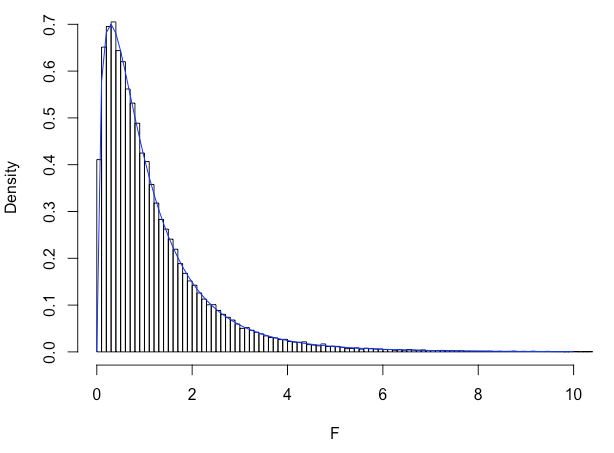
\includegraphics[width=0.85\linewidth]{_images/SamplingDistribF} 

}

\caption{Sampling distribution empirica per F, con l'ipotesi nulla vera, per l'esempio}\label{fig:figName91}
\end{figure}

Di conseguenza, possiamo evitare la simulazione Monte Carlo ed utilizzare la F di Fisher per calcolare la probabilità di ottenere un valore di F altrettanto estremo o più estremo del nostro. Ad esempio, in R, possiamo utilizzare la funzione:

\begin{Shaded}
\begin{Highlighting}[]
\KeywordTok{pf}\NormalTok{(}\FloatTok{23.663}\NormalTok{, }\DecValTok{3}\NormalTok{, }\DecValTok{12}\NormalTok{, }\DataTypeTok{lower.tail =}\NormalTok{ F)}
\CommentTok{## [1] 2.508789e-05}
\end{Highlighting}
\end{Shaded}

che porta ad un risultato molto simile a quello ottenuto con la simulazione di Monte Carlo. Insomma, in assenza di un effetto del trattamento (quindi per il solo effetto del caso), se ripetiamo l'esperimento infinite volte, abbiamo una probabilità molto bassa che si produca un valore di F altrettanto alto o più alto di quello da noi osservato.

Di conseguenza, se rifiutiamo l'ipotesi nulla di assenza di effetto del trattamento e accettiamo l'ipotesi alternativa (il trattamento ha avuto effetto significativo) ci portiamo dietro un rischio di errore estremamente piccolo, comunque molto al disotto della soglia prefissata del 5\%.

\hypertarget{operazioni-con-r}{%
\section{Operazioni con R}\label{operazioni-con-r}}

La stima dei parametri di un modello lineare, in R, può essere eseguita in modo molto banale, utilizzando la funzione `lm()' Il codice è il seguente:

\begin{Shaded}
\begin{Highlighting}[]
\NormalTok{mod <-}\StringTok{ }\KeywordTok{lm}\NormalTok{(Weight }\OperatorTok{~}\StringTok{ }\KeywordTok{factor}\NormalTok{(Treat), }\DataTypeTok{data =}\NormalTok{ dataset)}
\end{Highlighting}
\end{Shaded}

Il primo argomento rappresenta il modello lineare che vogliamo adattare ai dati: l'incusione dell'intercetta, codificata con il carattere `1' è opzionale (`Weight \textasciitilde{} 1 + Treat' e `Weight \textasciitilde{} Treat' sono equivalenti), mentre il termine stocastico \(\epsilon\) viene incluso di default e non deve essere indicato. Il termine `factor' sta a significare che la variabile `Treat' è un fattore sperimentale; questa specifica è opzionale quando la variabile è di tipo `carattere' (come in questo caso), ma è fondamentale quando abbiamo a che fare con una variabile a codifica numerica.

Una volta operato l'adattamento, l'oggetto `mod' contiene tutti i risultati, che possiamo ottenere con opportuni `estrattori'. Ad esempio, la funzione `summary()' restituisce le stime dei parametri:

\scriptsize

\begin{Shaded}
\begin{Highlighting}[]
\KeywordTok{summary}\NormalTok{(mod)}
\CommentTok{## }
\CommentTok{## Call:}
\CommentTok{## lm(formula = Weight ~ factor(Treat), data = dataset)}
\CommentTok{## }
\CommentTok{## Residuals:}
\CommentTok{##    Min     1Q Median     3Q    Max }
\CommentTok{## -6.360 -2.469  0.380  2.567  6.025 }
\CommentTok{## }
\CommentTok{## Coefficients:}
\CommentTok{##                             Estimate Std. Error t value Pr(>|t|)    }
\CommentTok{## (Intercept)                    9.175      1.959   4.684 0.000529 ***}
\CommentTok{## factor(Treat)Mixture_378      -4.047      2.770  -1.461 0.169679    }
\CommentTok{## factor(Treat)Rimsulfuron_30    7.685      2.770   2.774 0.016832 *  }
\CommentTok{## factor(Treat)Unweeded         17.598      2.770   6.352 3.65e-05 ***}
\CommentTok{## ---}
\CommentTok{## Signif. codes:  0 '***' 0.001 '**' 0.01 '*' 0.05 '.' 0.1 ' ' 1}
\CommentTok{## }
\CommentTok{## Residual standard error: 3.918 on 12 degrees of freedom}
\CommentTok{## Multiple R-squared:  0.8554, Adjusted R-squared:  0.8193 }
\CommentTok{## F-statistic: 23.66 on 3 and 12 DF,  p-value: 2.509e-05}
\end{Highlighting}
\end{Shaded}

\normalsize

Notiamo immediatamente che viene utilizzata la parametrizzazione con vincolo sul trattamento, visto che l'intercetta coincide con la media del primo trattamento. I valori di \(\alpha\) non sono altro che differenze tra questa media e tutte le altre medie.

I valori attesi e i residui possono essere ottenuti, in R, applicando due metodi `fitted()' e `residuals()' all'oggetto ottenuto dal fitting:

\begin{Shaded}
\begin{Highlighting}[]
\NormalTok{attesi <-}\StringTok{ }\KeywordTok{fitted}\NormalTok{(mod)}
\NormalTok{epsilon <-}\StringTok{ }\KeywordTok{residuals}\NormalTok{(mod)}
\end{Highlighting}
\end{Shaded}

La devianza del residuo (somma dei quadrati degli scarti) è:

\begin{Shaded}
\begin{Highlighting}[]
\KeywordTok{deviance}\NormalTok{(mod)}
\CommentTok{## [1] 184.1774}
\end{Highlighting}
\end{Shaded}

ementre la deviazione standard del residuo (\(\sigma\)), già visualizzabile nell'output della funzione `summary()', può essere estratta come:

\begin{Shaded}
\begin{Highlighting}[]
\KeywordTok{summary}\NormalTok{(mod)}\OperatorTok{$}\NormalTok{sigma}
\CommentTok{## [1] 3.917668}
\end{Highlighting}
\end{Shaded}

La tabella finale dell'ANOVA può essere ottenuta in R utilizzando la seguente funzione:

\begin{Shaded}
\begin{Highlighting}[]
\KeywordTok{anova}\NormalTok{(mod)}
\CommentTok{## Analysis of Variance Table}
\CommentTok{## }
\CommentTok{## Response: Weight}
\CommentTok{##               Df  Sum Sq Mean Sq F value    Pr(>F)    }
\CommentTok{## factor(Treat)  3 1089.53  363.18  23.663 2.509e-05 ***}
\CommentTok{## Residuals     12  184.18   15.35                      }
\CommentTok{## ---}
\CommentTok{## Signif. codes:  0 '***' 0.001 '**' 0.01 '*' 0.05 '.' 0.1 ' ' 1}
\end{Highlighting}
\end{Shaded}

\hypertarget{medie-marginali-attese}{%
\section{Medie marginali attese}\label{medie-marginali-attese}}

Abbiamo visto che le somme \(\mu + \alpha_j\) restituiscono le medie dei trattamenti e prendono il nome di \textbf{medie marginali attese}. Quando l'esperimento è bilanciato (ugual numero di repliche per ogni trattamento), esse sono uguali alle medie aritmetiche di ogni gruppo, mentre, quando l'esperimento è sbilanciato esso sono diverse, ma costituiscono una stima migliore delle medie delle popolazioni da cui i gruppi sono estratti rispetto alle medie aritmetiche. In R, il metodo più semplice per calcolare le medie marginali attese è quello di utilizzare la funzione `emmeans()', nel package `emmeans' (Lenth, 2016), che deve essere preventivamente installato e caricato in memoria.

\begin{Shaded}
\begin{Highlighting}[]
\CommentTok{#install.packages("emmeans") # Installare il package}
\KeywordTok{library}\NormalTok{(emmeans) }\CommentTok{#Caricare il package in memoria}
\NormalTok{medie <-}\StringTok{ }\KeywordTok{emmeans}\NormalTok{(mod, }\OperatorTok{~}\NormalTok{Treat)}
\NormalTok{medie}
\CommentTok{##  Treat           emmean   SE df lower.CL upper.CL}
\CommentTok{##  Metribuzin__348   9.18 1.96 12     4.91     13.4}
\CommentTok{##  Mixture_378       5.13 1.96 12     0.86      9.4}
\CommentTok{##  Rimsulfuron_30   16.86 1.96 12    12.59     21.1}
\CommentTok{##  Unweeded         26.77 1.96 12    22.50     31.0}
\CommentTok{## }
\CommentTok{## Confidence level used: 0.95}
\end{Highlighting}
\end{Shaded}

\hypertarget{per-concludere}{%
\section{Per concludere \ldots{}}\label{per-concludere}}

\begin{enumerate}
\def\labelenumi{\arabic{enumi}.}
\tightlist
\item
  Con l'ANOVA la variabilità totale dei dati viene decomposta in due quote, una attribuibile al trattamento sperimentale ed una inspiegabile (residuo)
\item
  L'effetto del trattamento è significativo, se la variabilità che esso provoca è superiore a quella inspiegabile
\item
  Il confronto tra varianze viene impostato sotto forma di rapporto (F).
\item
  L'ipotesi nulla è che il trattamento NON HA AVUTO effetto significativo
\item
  Sotto questa ipotesi nulla, l'F osservato ha una distribuzione F di Fisher
\item
  L'ipotesi nulla è rifiutata quando P \(\leq\) 0.05 (livello di protezione arbitrario, ma universalmente accettato)
\end{enumerate}

Ovviamente, è necessario ricordare che tutte le considerazioni fatte finora sono valide se il dataset è conforme alle assunzioni di base per l'ANOVA, per cui bisogna sempre eseguire i necessari controlli, di cui parleremo nel prossimo capitolo.

\begin{center}\rule{0.5\linewidth}{\linethickness}\end{center}

\hypertarget{per-approfondire-un-po-5}{%
\section{Per approfondire un po'\ldots{}}\label{per-approfondire-un-po-5}}

\hypertarget{simulazione-della-sampling-distribution-per-f}{%
\subsection{\texorpdfstring{Simulazione della \emph{sampling distribution} per F}{Simulazione della sampling distribution per F}}\label{simulazione-della-sampling-distribution-per-f}}

Di seguito forniamo il codice per simulare la \emph{sampling distribution} per F, quando l'ipotesi nulla è vera. Il codice impiega un generatore di numeri casuali gaussiano per ottenere dataset nei quali l'ipotesi nulla è vera, perché non vi è effetto del trattamento.

\begin{verbatim}
Fvals <- c()
set.seed(1234)
for(i in 1:100000){
  Ysim <- rnorm(16, 14.48375, 3.9177)
  Fvals[i] <- anova ( lm(Ysim ~ factor(Treat), data = dataset))$F[1]
}
min(Fvals)
max(Fvals)
length(Fvals[Fvals > 23.663])
\end{verbatim}

I risultati ottenuti sono quelli esposti più sopra

\hypertarget{altre-letture-3}{%
\subsection{Altre letture}\label{altre-letture-3}}

\begin{enumerate}
\def\labelenumi{\arabic{enumi}.}
\tightlist
\item
  Faraway, J.J., 2002. Practical regression and Anova using R. \url{http://cran.r-project.org/doc/contrib/Faraway-PRA.pdf}, R.
\item
  Fisher, Ronald (1918). ``Studies in Crop Variation. I. An examination of the yield of dressed grain from Broadbalk'' (PDF). Journal of Agricultural Science. 11 (2): 107--135.
\item
  Kuehl, R. O., 2000. Design of experiments: statistical principles of research design and analysis. Duxbury Press (CHAPTER 2)
\item
  Lenth, R.V., 2016. Least-Squares Means: The R Package lsmeans. Journal of Statistical Software 69. \url{https://doi.org/10.18637/jss.v069.i01}
\end{enumerate}

\hypertarget{la-verifica-delle-assunzioni-di-base}{%
\chapter{La verifica delle assunzioni di base}\label{la-verifica-delle-assunzioni-di-base}}

Nel momento in cui eseguiamo test d'ipotesi nell'ambito di un modello lineare, assumiamo implicitamente che i dati rispondano ai seguenti requisiti:

\begin{enumerate}
\def\labelenumi{\arabic{enumi}.}
\tightlist
\item
  il modello è corretto;
\item
  la risposta osservata è una funzione del modello più o meno l'errore sperimentale;
\item
  l' errore sperimentale è indipendente dal modello;
\item
  gli errori sono normalmente distribuiti, con media zero e varianze omogenee;
\item
  gli errori rilevati in esperimenti ripetuti sono tra loro indipendenti.
\item
  non ci sono osservazioni aberranti;
\end{enumerate}

Il rispetto di alcune di queste assunzioni di base è garantito dal disegno sperimentale, con il quale, attraverso la randomizzazione, si cerca di evitare ogni possibile confusione tra effetti deterministici ed errore sperimentale e si fa in modo che le osservazioni siano indipendenti tra di loro. Eventuali vincoli alla randomizzazione introdotti in fase di disegno (es. blocking) vengono gestiti con l'adozione di un modello ANOVA che ne riconosca l'esistenza (vderemo, ad esempio, l'ANOVA a blocchi randomizzati).

Ci sono tuttavia alcune assunzioni di base che possono essere verificate solo \emph{a posteriori}, cioè dopo aver effettuato la stima dei parametri. Queste assunzioni riguardano la struttura dei residui, che debbono essere normalmente distribuiti, omoscedastici e non debbono contenere valori aberranti. Ovviamente, per ottenere i residui, devo prima procedere al fitting del modello, individuare i valori attesi e quantificare il loro scostamento rispetto alle osservazioni.

Il rispetto delle assunzioni di base è importante, perché ogni deviazione può inficiare la validità dei test d'ipotesi e delle inferenze in genere, modificando il livello di significatività.

\hypertarget{procedure-diagnostiche}{%
\section{Procedure diagnostiche}\label{procedure-diagnostiche}}

Per diagnosticare eventuali patologie dei dati, possiamo utilizzare diverse procedure, così classificate:

\begin{enumerate}
\def\labelenumi{\arabic{enumi}.}
\tightlist
\item
  metodi grafici
\item
  metodi formali, tramite test d'ipotesi
\end{enumerate}

\hypertarget{analisi-grafica-dei-residui}{%
\section{Analisi grafica dei residui}\label{analisi-grafica-dei-residui}}

La gran parte dei pre-requisiti fondamentali di un dataset riguardano la struttura dei residui e, di conseguenza, l'ispezione grafica di questi ultimi, eventualmente accompagnata da semplici strumenti algebrici, possono permetterci di evidenziare la gran parte delle 'patologie' di cui soffrono i dati sperimentali. Si può affermare che l'ispezione dei residui è uno strumento diagnostico fondamentale, il cui impiego dovrebbe rientrare tra le metodiche di routine per ogni elaborazione statistica dei dati.

Ricordo che i residui sono gli scostamenti tra i valori osservati e quelli attesi sulla base del modello in studio; hanno sempre media 0, mentre la deviazione standard cambia di volta in volta.

\hypertarget{grafico-dei-residui-contro-i-valori-attesi}{%
\subsection{Grafico dei residui contro i valori attesi}\label{grafico-dei-residui-contro-i-valori-attesi}}

Il metodo grafico più utilizzato per l'analisi dei residui consiste nel plottare i residui verso i valori attesi. Se non vi sono problemi, i punti nel grafico dovrebbero essere distribuiti in modo assolutamente casuale, come in figura \ref{fig:figName101}.

\begin{figure}

{\centering 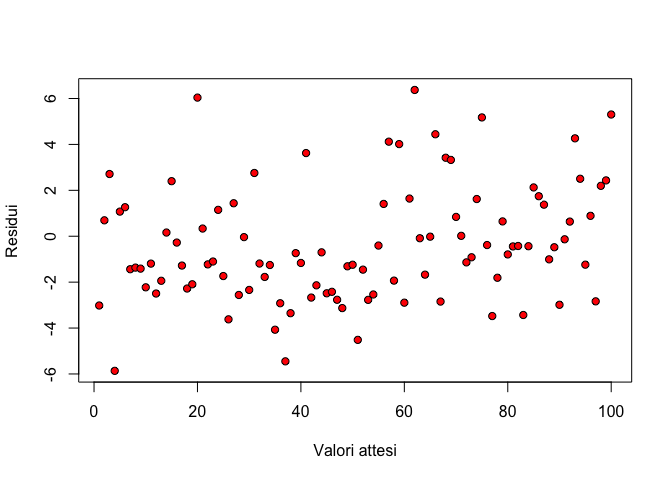
\includegraphics[width=0.85\linewidth]{_main_files/figure-latex/figName101-1} 

}

\caption{Grafico dei residui verso gli attesi: non è visibile nessuna deviazione rispetto agli assunti di base dei modelli lineari}\label{fig:figName101}
\end{figure}

Le osservazioni aberranti (\emph{outliers}) sono chiaramente indicate nel grafico dei residui come punti isolati rispetto agli altri (Figura \ref{fig:figName102}).

\begin{figure}

{\centering 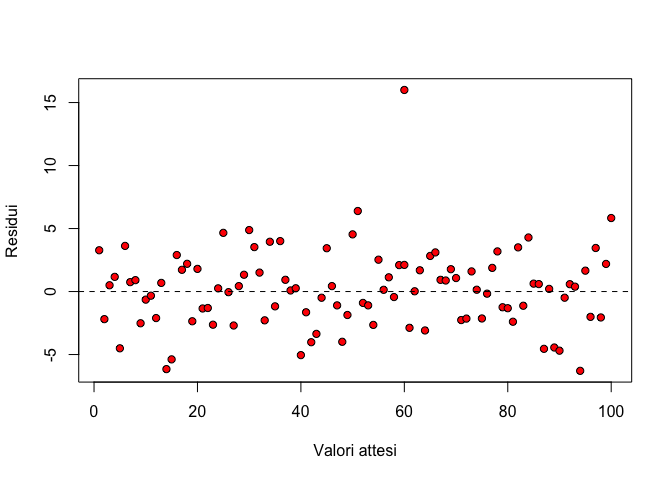
\includegraphics[width=0.85\linewidth]{_main_files/figure-latex/figName102-1} 

}

\caption{Grafico dei residui verso gli attesi: presenza di un dato aberrante}\label{fig:figName102}
\end{figure}

L'eterogeneità delle varianze è invece indicata da residui che si allargano o si stringono procedendo verso i margini del grafico (Figura \ref{fig:figName103}), facendo emergere una sorta di proporzionalità tra media e varianza.

\begin{figure}

{\centering 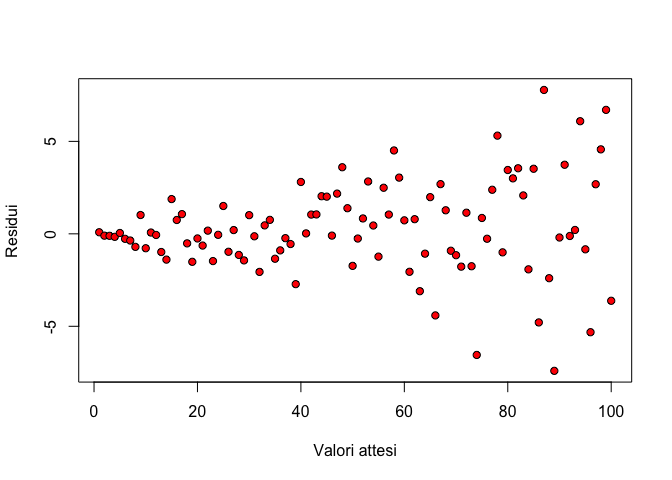
\includegraphics[width=0.85\linewidth]{_main_files/figure-latex/figName103-1} 

}

\caption{Grafico dei residui verso gli attesi: esempio di eteroscedasticità}\label{fig:figName103}
\end{figure}

A volte la relazione causa effetto non è lineare o, comunque, il modello devia sistematicamente dai dati osservati. Di conseguenza, i residui mostrano un evidente pattern legato al segno. Ad esempio, nella figura \ref{fig:figName104} i residui sono tendenzialmente negativi per bassi valori attesi e positivi per alti valori.

\begin{figure}

{\centering 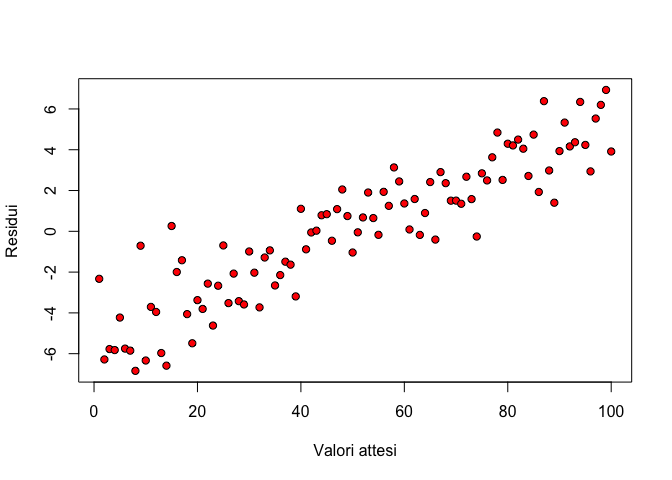
\includegraphics[width=0.85\linewidth]{_main_files/figure-latex/figName104-1} 

}

\caption{Grafico dei residui verso gli attesi: esempio di lack of fit (nonlinearità)}\label{fig:figName104}
\end{figure}

\hypertarget{qq-plot}{%
\subsection{QQ-plot}\label{qq-plot}}

Il grafico dei residui verso i valori attesi non è in grado di evidenziare problemi di non-normalità. A questo fine, risulta molto utile un QQ-plot (quantile-quantile plot), nel quale i residui \emph{standardizzati} vengono plottati contro i rispettivi percentili di una distribuzione normale standardizzata. Se la distribuzione dei dati è effettivamente normale, le due grandezze (i percentili nel campione e i percentili di una distribuzione normale standardizzata) dovrebbero essere largamente coincidenti; ad esempio, se la distribuzione è normale i residui negativi dovrebbero essere più o meno ugualmente numerosi di quelli positivi e non ci dovrebbero essere residui troppo alti in valore asoluto, soprattutto se il dataset è piccolo (infatti i valori estremi sono rari e dovrebbero comparire di rado). Se questo è vero, il QQ-plot dovrebbe essere costituito da punti che giacciono lungo la bisettrice del primo e del terzo quadrante (\ref{fig:figName105})

\begin{figure}

{\centering 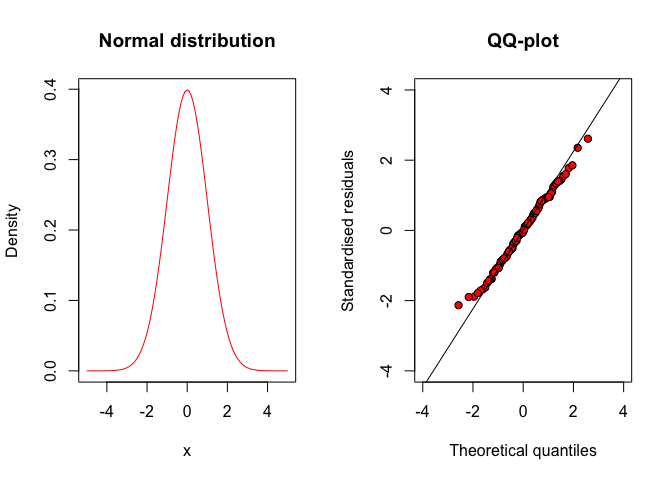
\includegraphics[width=0.85\linewidth]{_main_files/figure-latex/figName105-1} 

}

\caption{QQ-plot per un dataset normalmente distribuito}\label{fig:figName105}
\end{figure}

Le deviazioni più diffuse dalla normalità sono relative alla simmetria (skewness) e alla curtosi della popolazione. In particolare, può capitare che i residui abbiano asimmetria positiva (right-skewed: la media è maggiore della mediana), così che quelli negativi sono più numerosi di quelli positivi, ma questi ultimi sono mediamente di più elevato valore assoluto. Ad esempio, una distribuzione log-normale centrata è right-skewed ed, estraendo da questa una serie di valori, il QQ-plot si presenta come in figura \ref{fig:figName106}.

\begin{figure}

{\centering 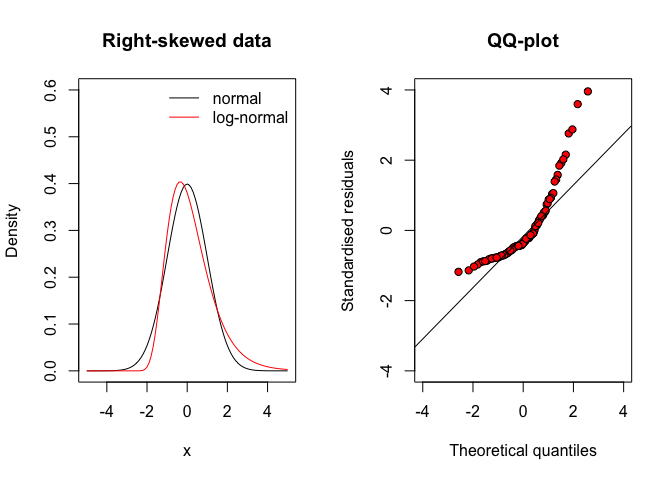
\includegraphics[width=0.85\linewidth]{_main_files/figure-latex/figName106-1} 

}

\caption{QQ-plot per un dataset con asimmetria positiva (right-skewed)}\label{fig:figName106}
\end{figure}

Al contrario, in una distribuzione left-skewed (asimmetria negativa), la media è minore della mediana e, di conseguenza, i residui positivi sono più numerosi, ma di valore assoluto più basso che non nella distribuzione normale corrispondente. Ad esempio, una distribuzione beta, in certe condizioni ( traslazione, alto \(a\) e basso \(b\)), è left-skewed e i valori campionati presentano un QQ-plot con un andamento tipico (\ref{fig:figName107}):

\begin{figure}

{\centering 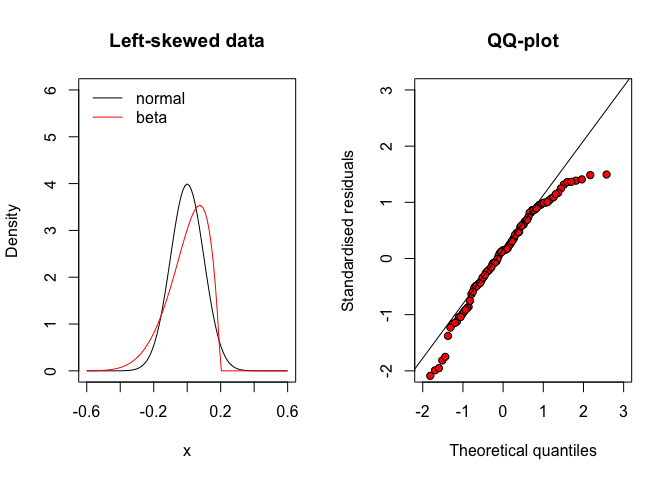
\includegraphics[width=0.85\linewidth]{_main_files/figure-latex/figName107-1} 

}

\caption{QQ-plot per un dataset con asimmetria negativa (left-skewed)}\label{fig:figName107}
\end{figure}

Per quanto riguarda la curtosi, è necessario osservare le code della distribuzione: se queste sono più alte di una distribuzione normale parliamo di distribuzione platicurtica, mentre se sono più basse parliamo di distribuzione leptocurtica. Ad esempio, una distribuzione di t di Student con pochi gradi di libertà è platicurtica ed il QQ-plot mostra l'andamento indicato in figura \ref{fig:figName108}.

\begin{figure}

{\centering 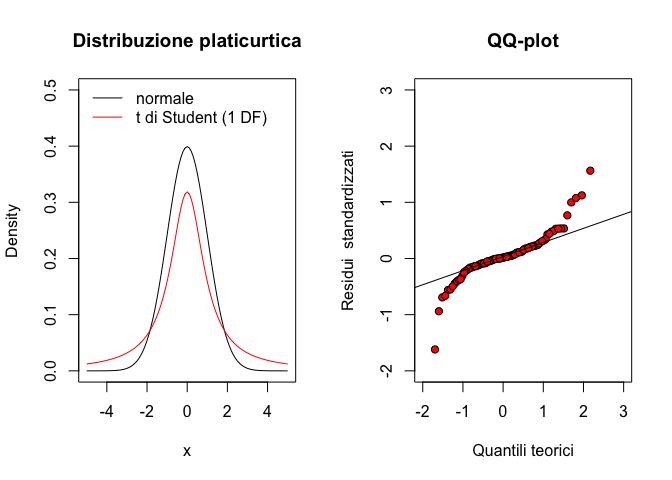
\includegraphics[width=0.85\linewidth]{_main_files/figure-latex/figName108-1} 

}

\caption{QQ-plot per un dataset con distribuzione platicurtica}\label{fig:figName108}
\end{figure}

Al contrario, una distribuzione uniforme in un intervallo ristretto è tipicamente leptocurtica e presenta un QQ-plot come quello riportato in Figura \ref{fig:figName109}.

\begin{figure}

{\centering 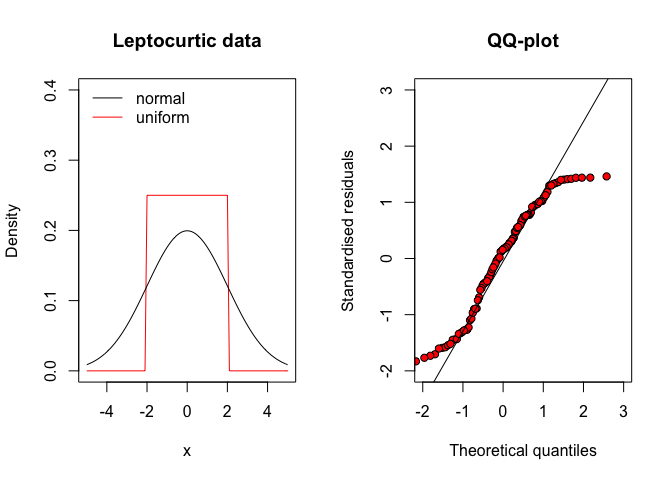
\includegraphics[width=0.85\linewidth]{_main_files/figure-latex/figName109-1} 

}

\caption{QQ-plot per un dataset con distribuzione leptocurtica}\label{fig:figName109}
\end{figure}

\hypertarget{strumenti-diagnostici-formali}{%
\section{Strumenti diagnostici formali}\label{strumenti-diagnostici-formali}}

La valutazioni precedentemente esposte sono di tipo grafico e sono considerate sufficientemente robuste per la maggior parte delle situazioni. Tuttavia, esistono anche test statistici che consentono di saggiare l'ipotesi nulla di 'assenza di deviazioni'. Con questi test, basta guardare il 'p-value': se questo è inferiore a 0.05 l'ipotesi nulla deve essere rifiutata e può essere necessario intraprendere azioni correttive.

Per l'omogeneità delle varianze veniva utilizzato il test di Bartlett, che, tuttavia, è oggi caduto in disuso, data la sua sensibilità alla non-normalità dei residui, quasi sempre presente, insieme all'eteroscedasticità. Oggi si preferisce utilizzare il test di Levene, che consiste nel sottoporre ad ANOVA i residui in valore assoluto, al posto dei dati osservati. Per ogni trattamento, i residui hanno media zero, ma se vengono presi in valore assoluto, hanno medie più alte quando la loro varianza è alta. Per esempio, possiamo prendere due campioni centrati, con media zero a varianza rispettivamente pari a 1 e 4:

\begin{Shaded}
\begin{Highlighting}[]
\NormalTok{A <-}\StringTok{ }\KeywordTok{c}\NormalTok{(}\OperatorTok{-}\DecValTok{1}\NormalTok{, }\DecValTok{0}\NormalTok{, }\DecValTok{1}\NormalTok{); B <-}\StringTok{ }\KeywordTok{c}\NormalTok{(}\OperatorTok{-}\DecValTok{4}\NormalTok{, }\DecValTok{0}\NormalTok{, }\DecValTok{4}\NormalTok{)}
\KeywordTok{mean}\NormalTok{(A); }\KeywordTok{mean}\NormalTok{(B)}
\CommentTok{## [1] 0}
\CommentTok{## [1] 0}
\KeywordTok{var}\NormalTok{(A); }\KeywordTok{var}\NormalTok{(B)}
\CommentTok{## [1] 1}
\CommentTok{## [1] 16}
\end{Highlighting}
\end{Shaded}

Se prendiamo i valori assoluti, la media del primo campione è 2/3, mentra la media del secondo campione è 8/3. Se questa differenza è significativa, essa produce il rifiuto dell'ipotesi nulla nel test F di ANOVA e conferma l'eterogeneità delle varianze. Il test di Levene, in R, si può eseguire con la funzione `leveneTest()' nel package `car'.

\begin{Shaded}
\begin{Highlighting}[]
\NormalTok{res <-}\StringTok{ }\KeywordTok{c}\NormalTok{(A, B)}
\NormalTok{tratt <-}\StringTok{ }\KeywordTok{rep}\NormalTok{(}\KeywordTok{c}\NormalTok{(}\StringTok{"A"}\NormalTok{, }\StringTok{"B"}\NormalTok{), }\DataTypeTok{each =} \DecValTok{3}\NormalTok{)}
\NormalTok{model <-}\StringTok{ }\KeywordTok{lm}\NormalTok{(res }\OperatorTok{~}\StringTok{ }\KeywordTok{factor}\NormalTok{(tratt))}
\KeywordTok{anova}\NormalTok{(model)}
\CommentTok{## Analysis of Variance Table}
\CommentTok{## }
\CommentTok{## Response: res}
\CommentTok{##               Df Sum Sq Mean Sq F value Pr(>F)}
\CommentTok{## factor(tratt)  1      0     0.0       0      1}
\CommentTok{## Residuals      4     34     8.5}
\NormalTok{car}\OperatorTok{::}\KeywordTok{leveneTest}\NormalTok{(res }\OperatorTok{~}\StringTok{ }\KeywordTok{factor}\NormalTok{(tratt), }\DataTypeTok{center=}\NormalTok{mean)}
\CommentTok{## Levene's Test for Homogeneity of Variance (center = mean)}
\CommentTok{##       Df F value Pr(>F)}
\CommentTok{## group  1  2.1176 0.2193}
\CommentTok{##        4}
\end{Highlighting}
\end{Shaded}

Il test di Levene può anche essere effettuato considerando gli scarti rispetto alla mediana (invece che alla media), in modo da ottenere un test più robusto nei confronti degli outliers.

Per quanto riguarda le deviazioni dalla normalità, può essere
utilizzato il test di Shapiro-Wilks. Per esempio, nel caso di un dataset ottenuto da una distribuzione uniforme (quindi non-normale), il test di Shapiro porta ai risultati sotto indicati.

\begin{Shaded}
\begin{Highlighting}[]
\KeywordTok{shapiro.test}\NormalTok{(}\KeywordTok{runif}\NormalTok{(}\DecValTok{100}\NormalTok{, }\DataTypeTok{min =} \DecValTok{-2}\NormalTok{, }\DataTypeTok{max =} \DecValTok{2}\NormalTok{))}
\CommentTok{## }
\CommentTok{##  Shapiro-Wilk normality test}
\CommentTok{## }
\CommentTok{## data:  runif(100, min = -2, max = 2)}
\CommentTok{## W = 0.94547, p-value = 0.0004227}
\end{Highlighting}
\end{Shaded}

\hypertarget{risultati-contraddittori}{%
\section{Risultati contraddittori}\label{risultati-contraddittori}}

La valutazione degli assunti di base è un passo fondamentale nell'analisi dei dati sperimentali è non deve mai essere dimenticata. Tuttavia, l'esperienza insegna che, nella pratica, è molto facile incontrare situazioni dubbie, nelle quali i risultati ottenuti con le diverse tecniche diagnostiche appaiono contraddittori e difficili da interpretare. Come comportarsi in questi casi? A mio parere bisogna sempre ricordare che la 'verità vera' ci sfugge e, di conseguenza, tutte le valutazioni debbono essere sempre condotte con il massimo 'buon senso'.

Un aspetto importante da considerare è la tipologia del dato: conteggi e proporzioni difficilmente sono normalmente distribuiti ed omoscedastici e, con questi dati, la prudenza non è mai troppa, quando si tratta di impiegare modelli lineari. Allo stesso modo, è necessaria una grande prudenza quando si analizzano variabili quantitative dove la differenza tra le diverse tesi è molto grande, orientativamente più di un ordine di grandezza. Con questi dati, l'assunzione di omogeneità delle varianze è quasi sempre violata.

\hypertarget{terapia}{%
\section{`Terapia'}\label{terapia}}

Se le procedure diagnostiche hanno evidenziato deviazioni rispetto agli assunti di base, è necessario valutare se e come intraprendere azioni correttive. Ovviamente, la `terapia' cambia al cambiare della `patologia'.

\hypertarget{correzionerimozione-degli-outliers}{%
\subsection{Correzione/Rimozione degli outliers}\label{correzionerimozione-degli-outliers}}

In presenza di outliers, la `terapia' più opportuna è, banalmente, quella di rimuoverli, ottenendo così un dataset `sbilanciato' (diverso numero di repliche per trattamento). Oggigiorno, trattare un dataset sbilanciato non costituisce un problema, ovviamente se si utilizzano le metodiche di analisi opportune. Qualche anno fa, al contrario, si cercava di evitare lo sbilanciamento a tutti i costi, utilizzando tecniche di imputing per l'immissione di valori 'ragionevoli' in sostituzione di quelli mancanti/aberranti. Con le dovute eccezioni, le tecniche di imputing sembrano oggi abbastanza obsolete.

Vorrei porre l'attenzione sul fatto che i dati aberranti sono dati molto `influenziali', nel senso che possono influenzare in modo molto marcato il risultato dell'analisi. Pertanto, se è sbagliato correggerli arbitrariamente, senza aver prima accertato che siano effettivamente frutto di errore, è altrettanto sbagliato lasciarli nel dataset. Ovviamente, la correzione non può che riguardare una larga minoranza dei dati sperimentali raccolti (uno o due dati), altrimenti si dovrà necessariamente pensare di ripetere l'esperimento.

\hypertarget{correzione-del-modello}{%
\subsection{Correzione del modello}\label{correzione-del-modello}}

Abbiamo visto che il modello impiegato potrebbe non essere adatto a descrivere il dataset (mancanza di adattamento). Gli effetti potrebbero non essere addittivi, ma moltiplicativi, oppure potrebbero essere non-lineari. Potrebbero essere presenti asintoti che il nostro modello non è in grado di descrivere, oppure la crescita/decrescita osservata potrebbero essere più lente/veloci di quanto la nostra funzione sia in grado di modellizzare. Per tutti questi casi, ovviamente, la strategia più consigliabile è quella di utilizzare un diverso modello, capace di descrivere meglio le osservazioni sperimentali.

\hypertarget{trasformazione-della-variabile-indipendente}{%
\subsection{Trasformazione della variabile indipendente}\label{trasformazione-della-variabile-indipendente}}

A volte la variabile dipendente non è qualitativa, bensì quantitativa. Vedremo meglio questo aspetto nei prossimi capitoli, quando parleremo di regressione. Tuttavia, anticipiamo che, quando la variabile indipendente è quantitativa, essa può essere sottoposta ad opportuna trasformazione. Ad esempio, se i dati mostrano un andamento esponenziale, la trasformazione della variabile indipendente in logaritmo può portare al sensibile miglioramento del fitting con un'equazione lineare.

\hypertarget{impiego-di-metodiche-statistiche-avanzate}{%
\subsection{Impiego di metodiche statistiche avanzate}\label{impiego-di-metodiche-statistiche-avanzate}}

In presenza di deviazioni sistematiche rispetto agli assunti di base, la cosa più logica sarebbe quella di chiedersi perché il dataset è non-normale e/o eteroscedastico ed incorporare queste informazioni nel modello. Ad esempio, un conteggio potrebbe seguire la distribuzione di Poisson, oppure una serie di proporzioni potrebbero seguire la distribuzione binomiale. In questi casi sarebbe opportuno utilizzare modelli lineari generalizzati (GLiM), basati non sulla distribuzione normale, ma su altre distribuzioni, più adatte per il fenomeno in studio. Allo stesso modo, l'eterogeneità delle varianze può essere incorporata nel modello, utilizzando tecniche dei minimi quadrati generalizzati (GLS). In altri casi, quando non si riescono a rispettare le assunzioni di base dei modelli, si può ricorrere a metodiche statistiche che ne fanno di menoe che, pertanto, sono dette metodiche `non-parametriche'.

In questo libro, non tratteremo né GLiM, né i GLs, né le metodiche non parametriche. Per quello che riguarda GLiM e GLS, si tratta di metodiche che richiedono un corso di livello più avanzato; per quanto riguarda le metodiche non-parametriche, di esse non parleremo, per una questione di preferenze personali: a mio modo di vedere, utilizzare metodiche non-parametriche è come rinuciare in partenza a comprendere le basi biologiche del fenomeno e le intrinseche relazioni causa-effetto che sussistono nella realtà.

\hypertarget{trasformazioni-stabilizzanti}{%
\subsection{Trasformazioni stabilizzanti}\label{trasformazioni-stabilizzanti}}

Una strategia empirica, ma molto seguita in pratica e caratterizzata da un'efficacia non disprezzabile, è quella di ricorrere alle trasformazioni correttive. Con questa tecnica, si va a cercare una metrica sulla quale le assunzioni di base dell'ANOVA siano rispettate e si esegue l'elaborazione dei dati trasformati invece che di quelli non trasformati.

Per i conteggi e per l'eterogeneità delle varianze di variabili continue, si consiglia la trasformazione in radice quadrata o in logaritmo, scegliendo in base a quella che consente la miglior distribuzione dei residui. Per le proporzioni, taluni consigliano la trasformazione nell'arcoseno della radice del valore, che è implementata nel package `aomisc', nella funzione `angularTransform()'. Questa funzione rivceve come input un valore percentuale e resituisce l'arcoseno della radice quadrata della proporzione corrispondente.

\begin{Shaded}
\begin{Highlighting}[]
\NormalTok{aomisc}\OperatorTok{::}\KeywordTok{angularTransform}\NormalTok{(}\KeywordTok{c}\NormalTok{(}\DecValTok{26}\NormalTok{, }\DecValTok{47}\NormalTok{, }\DecValTok{25}\NormalTok{, }\DecValTok{28}\NormalTok{, }\DecValTok{24}\NormalTok{))}
\CommentTok{## [1] 30.65730 43.28009 30.00000 31.94806 29.33387}
\end{Highlighting}
\end{Shaded}

Per evitare di schegliere la trasformazione `al buio', si può impiegare la procedura suggerita da Box e Cox (1964), basata su una `famiglia di trasformazioni', definita come segue:

\[ W = \left\{ \begin{array}{ll}
\frac{Y^\lambda}{\lambda - 1} & \quad \textrm{if} \,\,\, \lambda \neq 0 \\
\log(Y) & \quad \textrm{if} \,\,\, \lambda = 0
\end{array} \right. \]

dove W è la variabile trasformata, Y è la variabile originale e \(\lambda\) è il parametro che definisce la trasformazione. In particolare, osserviamo che se \(\lambda\) è pari ad 1 i dati non sono, di fatto, trasformati, se è pari a 0.5 abbiamo una trasformazione equivalente alla radice quadrata, se è pari a 0 abbiamo la trasformazione logaritmica, se è pari a -1 abbiamo una trasformazione equivalente al reciproco.

La scelta del valore \(\lambda\) può essere effettuata in modo empirico, confrontando la verosimiglianza di modelli basati su trasformazioni diverse. In R, questa procedura è automatizzata nella funzione `boxcox()', disponibile nel package MASS è verrà illustrata nell'esempio succesivo.

\hypertarget{esempio}{%
\section{Esempio}\label{esempio}}

Proviamo ad analizzare il dataset `insects', disponibile nel package `aomisc'. Si tratta di un dataset nel quale quindici piante sono state trattate con tre insetticidi diversi in modo completamente randomizzato, scegliendo cinque piante a caso per insetticida. Alcune settimane dopo il trattamento è stato rilevato il numero di insetti presenti su ciascuna pianta. Lasciando da parte le statistiche descrittive, eseguiamo subito l'ANOVA per questo dataset.

\begin{Shaded}
\begin{Highlighting}[]
\KeywordTok{library}\NormalTok{(aomisc)}
\KeywordTok{data}\NormalTok{(insects)}
\KeywordTok{head}\NormalTok{(insects)}
\CommentTok{##   Insecticide Rep Count}
\CommentTok{## 1           A   1   448}
\CommentTok{## 2           A   2   906}
\CommentTok{## 3           A   3   484}
\CommentTok{## 4           A   4   477}
\CommentTok{## 5           A   5   634}
\CommentTok{## 6           B   1   211}
\NormalTok{mod <-}\StringTok{ }\KeywordTok{lm}\NormalTok{(Count }\OperatorTok{~}\StringTok{ }\NormalTok{Insecticide, }\DataTypeTok{data =}\NormalTok{ insects)}
\end{Highlighting}
\end{Shaded}

Dopo aver effettuato l'ANOVA, i grafici dei residui possono essere ottenuti utilizzando la funzione `plot()' applicata al risultato del fitting lineare. L'argomento `which' specifica il tipo di grafico: se utilizziamo: `which = 1' otteniamo il grafico dei residui verso gli attesi, se invece utilizziamo `which = 2' otteniamo il QQ-plot. I due comandi sono:

\begin{verbatim}
plot(mod, which = 1)
plot(mod, which = 2)
\end{verbatim}

e forniscono l'output riportato in figura \ref{fig:figName110}.

\begin{figure}

{\centering 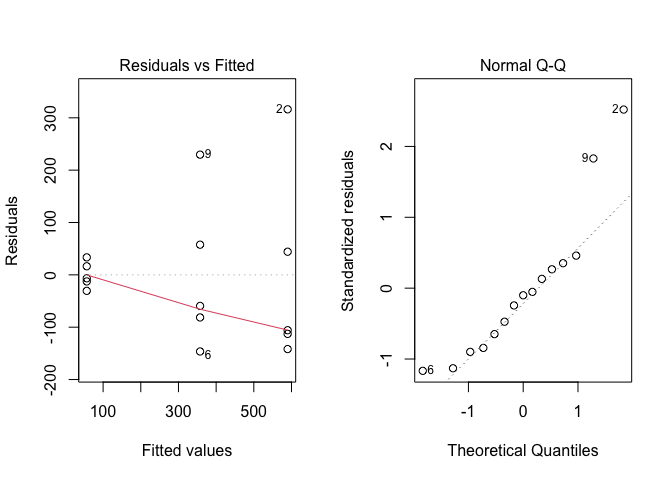
\includegraphics[width=0.85\linewidth]{_main_files/figure-latex/figName110-1} 

}

\caption{Analisi grafica dei residui per il dataset 'insects.csv'}\label{fig:figName110}
\end{figure}

Questo dataset mostra una chiara eteroscedasticità (vedi il grafico di sinistra) e qualche indizio di asimmetria positiva.

\begin{Shaded}
\begin{Highlighting}[]
\NormalTok{car}\OperatorTok{::}\KeywordTok{leveneTest}\NormalTok{(mod)}
\CommentTok{## Levene's Test for Homogeneity of Variance (center = median)}
\CommentTok{##       Df F value Pr(>F)}
\CommentTok{## group  2  1.0263 0.3878}
\CommentTok{##       12}
\KeywordTok{shapiro.test}\NormalTok{(}\KeywordTok{residuals}\NormalTok{(mod) )}
\CommentTok{## }
\CommentTok{##  Shapiro-Wilk normality test}
\CommentTok{## }
\CommentTok{## data:  residuals(mod)}
\CommentTok{## W = 0.87689, p-value = 0.04265}
\end{Highlighting}
\end{Shaded}

I test di Levene e Shapiro-Wilks confermano che la mancanza di normalità è significativa e, pertanto, scegliamo di impiegare una trasformazione correttiva. Utilizziamo quindi la funzione `boxcox()' per individuare la trasformazione più adatta a correggere la patologia riscontrata. Il comando è:

\begin{verbatim}
library(MASS)
boxcox(mod)
\end{verbatim}

e fornisce l'output in figura \ref{fig:figName111}.

\begin{figure}

{\centering 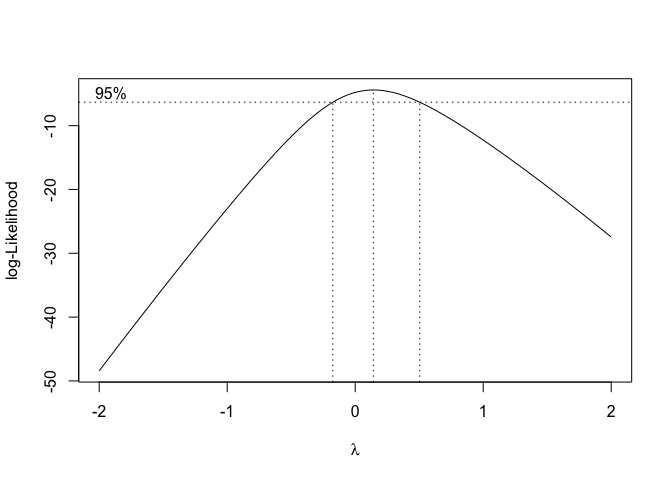
\includegraphics[width=0.85\linewidth]{_main_files/figure-latex/figName111-1} 

}

\caption{Scelta del valore ottimale di lambda per la trasformazione di Box e Cox}\label{fig:figName111}
\end{figure}

Vediamo che la verosimiglianza del modello raggiunge il massimo valore quando \(\lambda\) è pari a 0.14. I limiti dell'intervallo di confidenza vanno da poco sotto lo 0 a 0.5 circa. Rimanendo nell'ambito dell'intervallo di confidenza, scegliamo il valore \(\lambda = 0\), che corrisponde alla trasformazione logaritmica. Questa scelta è motivata dal fatto che si tratta di una trasformazione molto nota e facilmente comprensibile.

Pertanto, trasformiamo i dati nel logaritmo e ripetiamo l'ANOVA.

\begin{Shaded}
\begin{Highlighting}[]
\NormalTok{mod <-}\StringTok{ }\KeywordTok{lm}\NormalTok{(}\KeywordTok{log}\NormalTok{(Count) }\OperatorTok{~}\StringTok{ }\NormalTok{Insecticide, }\DataTypeTok{data =}\NormalTok{ insects)}
\KeywordTok{par}\NormalTok{(}\DataTypeTok{mfrow =} \KeywordTok{c}\NormalTok{(}\DecValTok{1}\NormalTok{,}\DecValTok{2}\NormalTok{))}
\KeywordTok{plot}\NormalTok{(mod, }\DataTypeTok{which =} \DecValTok{1}\NormalTok{)}
\KeywordTok{plot}\NormalTok{(mod, }\DataTypeTok{which =} \DecValTok{2}\NormalTok{)}
\end{Highlighting}
\end{Shaded}

\begin{figure}

{\centering 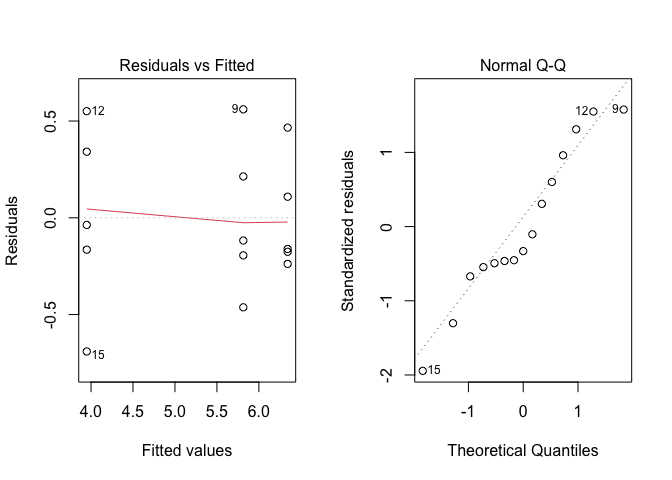
\includegraphics[width=0.85\linewidth]{_main_files/figure-latex/figName112-1} 

}

\caption{Analisi grafica dei residui per il dataset 'insects.csv', previa trasformazione logaritmica}\label{fig:figName112}
\end{figure}

Vediamo che i dati trasformati non mostrano più alcun sintomo di eteroscedasticità e, di conseguenza, l'ANOVA su questa metrica è totalmente affidabile. Ovviamente, avendo lavorato con il logaritmo dei dati, commentare i risultati potrebbe essere più complicato, in quanto dovremmo calcolare le medie marginali attese su scala logaritmica, come indicato nel codice sottostante.

\begin{Shaded}
\begin{Highlighting}[]
\KeywordTok{library}\NormalTok{(emmeans)}
\NormalTok{medie <-}\StringTok{ }\KeywordTok{emmeans}\NormalTok{(mod, }\OperatorTok{~}\NormalTok{Insecticide)}
\NormalTok{medie}
\CommentTok{##  Insecticide emmean    SE df lower.CL upper.CL}
\CommentTok{##  A             6.34 0.178 12     5.96     6.73}
\CommentTok{##  B             5.81 0.178 12     5.43     6.20}
\CommentTok{##  C             3.95 0.178 12     3.56     4.34}
\CommentTok{## }
\CommentTok{## Results are given on the log (not the response) scale. }
\CommentTok{## Confidence level used: 0.95}
\end{Highlighting}
\end{Shaded}

È evidente che presentare le medie su scala logaritmica potrebbe non essere di immediata o facile lettura. Per questo, potremmo pensare di retrotrasformare le medie, utilizzando la trasformazione inversa di quella logaritmica, cioè l'antilogaritmo. Ad esempio, per la prima media:

\[e^{6.34} = 566.7963\]

In questo modo la nostra unità di misura ridiventa quella originale, anche se il valore ottenuto non coincide con la media dei dati originali; in effetti la trasformazione è non lineare e la media dei logaritmi non può coincidere con il logaritmo della media. Possiamo osservare che la media del trattamento A, sulla scala originale, è:

\begin{Shaded}
\begin{Highlighting}[]
\KeywordTok{mean}\NormalTok{(insects[insects}\OperatorTok{$}\NormalTok{Insecticide }\OperatorTok{==}\StringTok{ "A"}\NormalTok{,}\StringTok{"Count"}\NormalTok{])}
\CommentTok{## [1] 589.8}
\end{Highlighting}
\end{Shaded}

e risulta più alta della media retrotrasformata. In realtà, se è vero che i logaritmi sono normalmente distribuiti, la media dei logaritmi (6.34) dovrebbe essere uguale alla mediana (ricordiamo che in una distribuzione normale media e mediana coincidono). La mediana è il valore centrale; dato che la retro-trasformazione è monotona, il valore centrale resta centrale, anche se io retrotrasformo. Quindi la media retrotrasformata è uno stimatore della mediana della popolazione originale, non della sua media. Questo non è uno svantaggio: infatti il QQ-plot suggerisce un'asimmetria positiva (confronta la Figura \ref{fig:figName111} con la Figura \ref{fig:figName106} cosa che è confermata dal fatto che la mediana è minore della media. Se la distribuzione dei dati è asimmetrica, la mediana è un indicatore di tendenza centrale migliore della media, perché meno sensibile ai valori estremi, che sono più frequenti in caso di asimmetria.

Il problema è che, se vogliamo utilizzare la media retrotrasformata, dobbiamo trovare un valore di errore standard per questo stima, con il quale esprimere la sua incertezza. In realtà, anche l'errore standard può essere retrotrasformato, con una tecnica detta metodo `delta', che costituisce un estensione della legge di propagazione degli errori per le trasformazioni non-lineari. È inutile andare nel dettaglio; diciamo solo che la funzione `emmeans()' rende semplicissima l'implementazione del metodo delta, con il comando seguente:

\begin{Shaded}
\begin{Highlighting}[]
\NormalTok{retroMedie <-}\StringTok{ }\KeywordTok{emmeans}\NormalTok{(mod, }\OperatorTok{~}\NormalTok{Insecticide, }\DataTypeTok{transform =} \StringTok{"response"}\NormalTok{)}
\NormalTok{retroMedie}
\CommentTok{##  Insecticide response     SE df lower.CL upper.CL}
\CommentTok{##  A              568.6 101.01 12    348.5      789}
\CommentTok{##  B              335.1  59.54 12    205.4      465}
\CommentTok{##  C               51.9   9.22 12     31.8       72}
\CommentTok{## }
\CommentTok{## Confidence level used: 0.95}
\end{Highlighting}
\end{Shaded}

Con questo abbiamo tutto quello che ci serve: stime ed errori standard, che, ovviamente, sono diversi per le diverse medie retrotrasformate, coerentemente con la mancanza di omoscedasticità.

\begin{center}\rule{0.5\linewidth}{\linethickness}\end{center}

\hypertarget{per-approfondire-un-po-6}{%
\section{Per approfondire un po' \ldots{}}\label{per-approfondire-un-po-6}}

\begin{enumerate}
\def\labelenumi{\arabic{enumi}.}
\tightlist
\item
  Ahrens, W. H., D. J. Cox, and G. Budwar. 1990, Use of the arcsin and square root trasformation for subjectively determined percentage data. Weed science 452-458.
\item
  Anscombe, F. J. and J. W. Tukey. 1963, The examination and analysis of residuals. Technometrics 5: 141-160.
\item
  Box, G. E. P. and D. R. Cox. 1964, An analysis of transformations. Journal of the Royal Statistical Society, B-26, 211-243, discussion 244-252.
\item
  D'Elia, A. 2001, Un metodo grafico per la trasformazione di Box-Cox: aspetti esplorativi ed inferenziali. STATISTICA LXI: 630-648.
\item
  Saskia, R. M. 1992, The Box-Cox transformation technique: a review. Statistician 41: 169-178.
\item
  Weisberg, S., 2005. Applied linear regression, 3rd ed. John Wiley \& Sons Inc. (per il metodo `delta')
\end{enumerate}

\hypertarget{contrasti-e-confronti-multipli}{%
\chapter{Contrasti e confronti multipli}\label{contrasti-e-confronti-multipli}}

La scomposizione della varianza (ANOVA fisheriana) rappresenta frequentemente il primo passo nell'elaborazione statistica dei dati sperimentali. Essa consente di quantificare l'errore sperimentale e ci permette di sapere se l'effetto del trattamento (nel suo complesso) è risultato significativo. Tuttavia, con la sola ANOVA non siamo ancora capaci di definire una graduatoria di merito tra i diversi livelli del trattamento sperimentale. Dopo l'ANOVA, è quindi logico chiedersi (in ordine crescente di importanza):

\begin{enumerate}
\def\labelenumi{\arabic{enumi}.}
\tightlist
\item
  Il generico trattamento A ha un effetto diverso dal trattamento B?
\item
  Il trattamento A è migliore/uguale/peggiore di B?
\item
  Quant'è la differenza tra A e B?
\end{enumerate}

La prima domanda è abbastanza sciocca, in quanto due trattamenti non sono quasi mai esattamente uguali. Le altre due domande sono invece più rilevanti, specialmente la seconda, in quanto conoscere l'entità della differenza, oltre che la sua significatività, è fondamentale per comprendere anche la sua rilevanza biologica. Infatti una differenza potrebbe essere significativa, ma irrilevante da un punto di vista agronomico o, viceversa, essa potrebbe essere non significativa, ma estremamente rilevante, quindi meritevole di ulteriori approfondimenti scientifici. Per rispondere alle domande precedenti, in genere, utilizziamo i \textbf{contrasti lineari}, che introdurremo con un esempio.

\hypertarget{esempio-1}{%
\section{Esempio}\label{esempio-1}}

Ammettiamo di aver effettuato una prova con un trattamento sperimentali caratterizzato da quattro livelli qualitativi (tesi di concimazione), con i risultati riportati di seguito:

\begin{Shaded}
\begin{Highlighting}[]
\NormalTok{yield <-}\StringTok{ }\KeywordTok{c}\NormalTok{(}\DecValTok{20}\NormalTok{,}\DecValTok{21}\NormalTok{,}\DecValTok{23}\NormalTok{,}\DecValTok{22}\NormalTok{,}\DecValTok{19}\NormalTok{,}\DecValTok{20}\NormalTok{,}\DecValTok{12}\NormalTok{,}\DecValTok{15}\NormalTok{,}\DecValTok{13}\NormalTok{,}\DecValTok{19}\NormalTok{,}\DecValTok{18}\NormalTok{,}\DecValTok{16}\NormalTok{)}
\NormalTok{fert <-}\StringTok{ }\KeywordTok{factor}\NormalTok{(}\KeywordTok{rep}\NormalTok{(}\KeywordTok{c}\NormalTok{(}\StringTok{"Minerale"}\NormalTok{, }\StringTok{"Minerale lento"}\NormalTok{, }
          \StringTok{"Non concimato"}\NormalTok{, }\StringTok{"Organico"}\NormalTok{), }\DataTypeTok{each=}\DecValTok{3}\NormalTok{))}
\NormalTok{dataset <-}\StringTok{ }\KeywordTok{data.frame}\NormalTok{(yield, fert)}
\KeywordTok{rm}\NormalTok{(yield, fert)}
\NormalTok{dataset}
\CommentTok{##    yield           fert}
\CommentTok{## 1     20       Minerale}
\CommentTok{## 2     21       Minerale}
\CommentTok{## 3     23       Minerale}
\CommentTok{## 4     22 Minerale lento}
\CommentTok{## 5     19 Minerale lento}
\CommentTok{## 6     20 Minerale lento}
\CommentTok{## 7     12  Non concimato}
\CommentTok{## 8     15  Non concimato}
\CommentTok{## 9     13  Non concimato}
\CommentTok{## 10    19       Organico}
\CommentTok{## 11    18       Organico}
\CommentTok{## 12    16       Organico}
\end{Highlighting}
\end{Shaded}

L'ANOVA può essere eseguita facilmente con R, utilizzando l'ormai nota funzione `lm()'.

\begin{Shaded}
\begin{Highlighting}[]
\NormalTok{model <-}\StringTok{ }\KeywordTok{lm}\NormalTok{(yield }\OperatorTok{~}\StringTok{ }\NormalTok{fert, }\DataTypeTok{data=}\NormalTok{dataset)}
\KeywordTok{anova}\NormalTok{(model)}
\CommentTok{## Analysis of Variance Table}
\CommentTok{## }
\CommentTok{## Response: yield}
\CommentTok{##           Df  Sum Sq Mean Sq F value    Pr(>F)    }
\CommentTok{## fert       3 115.000  38.333  16.429 0.0008821 ***}
\CommentTok{## Residuals  8  18.667   2.333                      }
\CommentTok{## ---}
\CommentTok{## Signif. codes:  0 '***' 0.001 '**' 0.01 '*' 0.05 '.' 0.1 ' ' 1}
\end{Highlighting}
\end{Shaded}

In questo caso, l'analisi della varianza ed il relativo test di F ci dicono che esiste una differenza significativa tra le medie, ma rimane il problema di classificare le soluzioni concimanti in ordine di efficacia. Chi è migliore di chi?

Per prima cosa, calcoliamo le medie dei trattamenti, utilizzando la funzione \emph{emmeans()} del package \emph{emmeans}:

\begin{Shaded}
\begin{Highlighting}[]
\KeywordTok{library}\NormalTok{(emmeans)}
\NormalTok{medie <-}\StringTok{ }\KeywordTok{emmeans}\NormalTok{(model, }\OperatorTok{~}\NormalTok{fert)}
\NormalTok{medie}
\CommentTok{##  fert           emmean    SE df lower.CL upper.CL}
\CommentTok{##  Minerale         21.3 0.882  8     19.3     23.4}
\CommentTok{##  Minerale lento   20.3 0.882  8     18.3     22.4}
\CommentTok{##  Non concimato    13.3 0.882  8     11.3     15.4}
\CommentTok{##  Organico         17.7 0.882  8     15.6     19.7}
\CommentTok{## }
\CommentTok{## Confidence level used: 0.95}
\end{Highlighting}
\end{Shaded}

Vediamo che l'output di R riporta anche gli errori standard delle medie (SEM) e gli intervalli di confidenza.

\hypertarget{i-contrasti}{%
\section{I contrasti}\label{i-contrasti}}

Si definisce CONTRASTO una combinazione lineare dei parametri di un modello (ad esempio le medie dei trattamenti), in modo che i coefficienti sommati diano 0. Ad esempio, considerando i parametri del modello precedente, una combinazione lineare del tipo:

\[C = \frac{1}{3} \cdot 21.33 + \frac{1}{3} \cdot 20.33 - 1 \cdot 13.33 + \frac{1}{3} \cdot 17.67 = 6.446667\]

è un contrasto, in quanto la somma dei coefficienti è:

\[C = \frac{1}{3} + \frac{1}{3} - 1 + \frac{1}{3} = 0\]

Al contrario una combinazione lineare del tipo:

\[C1 = 1 \cdot 21.33  + 1 \cdot 20.33 - 1 \cdot 13.33 + 1 \cdot 17.67\]

non è un contrasto valido, perché la somma dei coefficienti non è zero (1 + 1 - 1 + 1 = -2).

Il primo contrasto C, ha un preciso significato biologico, in quanto stima la differenza tra il non fertilizzato e la media dei fertilizzati. Il risultato è 6.45 e, con esso, possiamo rispondere a tutte e tre le domande elencato all'inizio:

\begin{enumerate}
\def\labelenumi{\arabic{enumi}.}
\tightlist
\item
  La fertilizzazione (in media) ha un effetto diverso dal testimone non fertilizzato? Risposta: si, perché la differenza è non nulla
\item
  La fertilizzazione in media è migliore/uguale/peggiore del testimone? Risposta: migliore, perché la differenza è positiva.
\item
  Quant'è la differenza tra il fertilizzato e il non-fertilizzato? Risposta: è pari a 6.45
\end{enumerate}

E' evidente, tuttavia, che l'errore sperimentale produce incertezza, che sarebbe bene includere nei risultati, sotto forma di deviazione standard (errore standard) del contrasto, oppure come intervallo di confidenza.

\hypertarget{varianza-del-contrasto-e-test-dipotesi}{%
\subsection{Varianza del contrasto e test d'ipotesi}\label{varianza-del-contrasto-e-test-dipotesi}}

Ogni contrasto ha la sua varianza, ottenuta come combinazione lineare di varianze, attraverso il metodo di propagazione degli errori. Considerando che le medie sono, usualmente, indipendenti, la varianza di un contrasto tra medie è:

\[\textrm{var}(A \mu_1 + B \mu_2) = (A \cdot \sigma_{\mu_1} )^{2}  + (B \cdot \sigma_{\mu_2} ) ^ 2\]

dove A e B sono i coefficienti del contrasto, \(\mu_1\) e \(\mu_2\) sono due medie e \(\sigma_{\mu_1}\) e \(\sigma_{\mu_2}\) sono gli errori standard di \(\mu_1\) e \(\mu_2\). Nel nostro caso, la varianza del contrasto è:

\[var(C) = \left( \frac{1}{3} \cdot 0.882 \right)^2 +  \left( \frac{1}{3} \cdot 0.882 \right)^2 + \left( 1 \cdot 0.882 \right)^2 +  \left( \frac{1}{3} \cdot 0.882 \right)^2 = 1.037\]

mentre la deviazione standard (cioè l'errore standard) del contrasto è pari a:

\[ ES(C) = \sqrt{1.037} = 1.0183\]

Insomma, per il contrasto C abbiamo una stima puntuale (6.45) e un errore standard (1.0183). Utilizzando questo errore standard possiamo calcolare l'intervallo di confidenza del contrasto, secondo le metodiche usuali che abbiamo gia visto in un capitolo precedente. Gli intervalli di confidenza dei contrasti sono trattati in modo più dettagliato in fondo al capitolo.

A questo punto potremmo chiederci: ``E' possibile che il contrasto, nella realtà, sia uguale a 0?''. Ovviamente è possibile: il nostro è solo un campione e, se ripetessimo il campionamento, potremmo ottenere valori di C totalmente diversi da quello effettivamente osservato. Poniamo l'ipotesi nulla in questi termini:

\[H_0: K = 0\]

dove \(K\) è il valore `vero' del contrasto, per le popolazioni che hanno generato i dati. Scriviamo la statistica:

\[T = \frac{C}{ES(C)} = \frac{6.45}{1.0183} = 6.331\]

Se l'ipotesi nulla è vera, che probabilità abbiamo di osservare T = 6.331? In generale, il rapporto tra una stima ed il suo errore standard ha una distribuzione t di Student, con un numero di gradi di libertà pari a quelli del residuo dell'ANOVA. Di conseguenza possiamo saggiare l'ipotesi nulla che il contrasto è uguale a 0 calcolando la probabilità di trovare un valore di T pari o superiore (in valore assoluto) a quello da noi ottenuto. Nell'esempio sottostante abbiamo moltiplicato la probabilità trovata per 2, dato che si tratta di un test a due code:

\begin{Shaded}
\begin{Highlighting}[]
\NormalTok{t <-}\StringTok{ }\FloatTok{6.4467} \OperatorTok{/}\StringTok{ }\FloatTok{1.018277}
\DecValTok{2} \OperatorTok{*}\StringTok{ }\KeywordTok{pt}\NormalTok{(t, }\DecValTok{8}\NormalTok{, }\DataTypeTok{lower.tail =}\NormalTok{ F)}
\CommentTok{## [1] 0.0002251554}
\end{Highlighting}
\end{Shaded}

Con questo abbiamo risposto a tutte e tre le nostre domande di ricerca:

\begin{enumerate}
\def\labelenumi{\arabic{enumi}.}
\tightlist
\item
  Fertilizzare non produce lo stesso effetto che non fertilizzare;
\item
  Fertilizzare permette di produrre di più che non fertilizzare
\item
  la differenza è pari a 6.45 q/ha e ci sono elementi sufficienti per ritenere che essa sia diversa da 0.
\end{enumerate}

\hypertarget{i-contrasti-con-r}{%
\subsection{I contrasti con R}\label{i-contrasti-con-r}}

Nel caso in esempio, si potrebbero pianificare tre contrasti (incluso quello già discusso):

\begin{enumerate}
\def\labelenumi{\arabic{enumi}.}
\tightlist
\item
  non concimato vs concimato (in media)
\item
  concime organico vs.~concimi minerali (in media)
\item
  minerale tradizionale vs.~lento rilascio.
\end{enumerate}

Per eseguire i contrasti con R, dobbiamo, in primo luogo, definire i vettori dei coefficienti. Per il primo contrasto, abbiamo già visto che questo vettore è:

\begin{Shaded}
\begin{Highlighting}[]
\NormalTok{m1 <-}\StringTok{ }\KeywordTok{c}\NormalTok{(}\DecValTok{1}\OperatorTok{/}\DecValTok{3}\NormalTok{, }\DecValTok{1}\OperatorTok{/}\DecValTok{3}\NormalTok{,  }\DecValTok{-1}\NormalTok{, }\DecValTok{1}\OperatorTok{/}\DecValTok{3}\NormalTok{)}
\end{Highlighting}
\end{Shaded}

Per gli altri due contrasti, i coefficienti sono:

\begin{Shaded}
\begin{Highlighting}[]
\NormalTok{m2 <-}\StringTok{ }\KeywordTok{c}\NormalTok{(}\FloatTok{0.5}\NormalTok{, }\FloatTok{0.5}\NormalTok{, }\DecValTok{0}\NormalTok{, }\DecValTok{-1}\NormalTok{)}
\NormalTok{m3 <-}\StringTok{ }\KeywordTok{c}\NormalTok{(}\DecValTok{1}\NormalTok{, }\DecValTok{-1}\NormalTok{, }\DecValTok{0}\NormalTok{, }\DecValTok{0}\NormalTok{)}
\end{Highlighting}
\end{Shaded}

Una volta definiti i coefficienti, possiamo utilizzare il package `emmeans', con la funzione `contrast()', passandole, come argomento, l'oggetto `medie', ottenuto con la funzione `emmeans()' (vedi sopra), ed una lista contenente i tre vettori dei coefficienti (m1, m2, m3), ai quali si può assegnare un nome, ad esempio, C1, C2 e C3.

\small

\begin{Shaded}
\begin{Highlighting}[]
\NormalTok{m1 <-}\StringTok{ }\KeywordTok{c}\NormalTok{(}\DecValTok{1}\OperatorTok{/}\DecValTok{3}\NormalTok{, }\DecValTok{1}\OperatorTok{/}\DecValTok{3}\NormalTok{,  }\DecValTok{-1}\NormalTok{, }\DecValTok{1}\OperatorTok{/}\DecValTok{3}\NormalTok{)}
\NormalTok{m2 <-}\StringTok{ }\KeywordTok{c}\NormalTok{(}\FloatTok{0.5}\NormalTok{, }\FloatTok{0.5}\NormalTok{, }\DecValTok{0}\NormalTok{, }\DecValTok{-1}\NormalTok{)}
\NormalTok{m3 <-}\StringTok{ }\KeywordTok{c}\NormalTok{(}\DecValTok{1}\NormalTok{, }\DecValTok{-1}\NormalTok{, }\DecValTok{0}\NormalTok{, }\DecValTok{0}\NormalTok{)}
\KeywordTok{contrast}\NormalTok{(medie, }\DataTypeTok{method=}\KeywordTok{list}\NormalTok{(}\DataTypeTok{C1=}\NormalTok{m1, }\DataTypeTok{C2=}\NormalTok{m2, }\DataTypeTok{C3=}\NormalTok{m3), }
           \DataTypeTok{adjust=}\StringTok{"none"}\NormalTok{)}
\CommentTok{##  contrast estimate   SE df t.ratio p.value}
\CommentTok{##  C1           6.44 1.02  8 6.328   0.0002 }
\CommentTok{##  C2           3.17 1.08  8 2.932   0.0189 }
\CommentTok{##  C3           1.00 1.25  8 0.802   0.4458}
\end{Highlighting}
\end{Shaded}

\normalsize

Il test mostra che la concimazione ha, in media, un effetto significativo, che il concime organico differisce significativamente dai minerali (in media) e che il concime a lento rilascio non è significativamente diverso da quello normale.

\hypertarget{i-confronti-multipli-a-coppie-pairwise-comparisons}{%
\section{I confronti multipli a coppie (pairwise comparisons)}\label{i-confronti-multipli-a-coppie-pairwise-comparisons}}

Non sempre le prove sperimentali consentono di saggiare pochi contrasti pre-stabiliti, ma spesso è necessario confrontare tutte le possibili coppie di trattamenti (\emph{pairwise comparisons}). In questo caso dovremmo definire un contrasto per ogni coppia di medie, anche se l'impiego del package `emmeans' agevola, non di poco, il lavoro.

In particolare, possiamo immaginare due situazioni di riferimento: tutti contro tutti (confronti tipo ``Tukey'') e tutti verso uno (confronti tipo ``Dunnett''). Questo secondo tipo di contrasto può essere interessante, nel nostro caso, per verificare quale dei concimi consenta un incremento di produzione rispetto al testimone non concimato, qualora non sia necessario confrontare tra di loro le tesi concimanti.

Nell'esempio sottostante mostriamo un confronto tipo Tukey (tutti contro tutti), eseguito utilizzando la funzione `contrast' (come sopra), passando il valore `pairwise' all'argomento `method'. Vediamo che ci sono sei contrasti a coppie.

\footnotesize

\begin{Shaded}
\begin{Highlighting}[]
\CommentTok{#Confronti multipli a coppie}
\KeywordTok{contrast}\NormalTok{(medie, }\DataTypeTok{adjust=}\StringTok{"none"}\NormalTok{, }\DataTypeTok{method=}\StringTok{"pairwise"}\NormalTok{)}
\CommentTok{##  contrast                       estimate   SE df t.ratio p.value}
\CommentTok{##  Minerale - Minerale lento          1.00 1.25  8  0.802  0.4458 }
\CommentTok{##  Minerale - Non concimato           8.00 1.25  8  6.414  0.0002 }
\CommentTok{##  Minerale - Organico                3.67 1.25  8  2.940  0.0187 }
\CommentTok{##  Minerale lento - Non concimato     7.00 1.25  8  5.612  0.0005 }
\CommentTok{##  Minerale lento - Organico          2.67 1.25  8  2.138  0.0650 }
\CommentTok{##  Non concimato - Organico          -4.33 1.25  8 -3.474  0.0084}
\end{Highlighting}
\end{Shaded}

\normalsize

Per i confronti del tipo `tutti verso uno' è possibile utilizzare la stessa funzione, assegnando però il valore `dunnett' (invece che `pairwise') all' argomento `method'.

\small

\begin{Shaded}
\begin{Highlighting}[]
\KeywordTok{contrast}\NormalTok{(medie, }\DataTypeTok{adjust=}\StringTok{"none"}\NormalTok{, }\DataTypeTok{method=}\StringTok{"dunnett"}\NormalTok{)}
\CommentTok{##  contrast                  estimate   SE df t.ratio p.value}
\CommentTok{##  Minerale lento - Minerale    -1.00 1.25  8 -0.802  0.4458 }
\CommentTok{##  Non concimato - Minerale     -8.00 1.25  8 -6.414  0.0002 }
\CommentTok{##  Organico - Minerale          -3.67 1.25  8 -2.940  0.0187}
\end{Highlighting}
\end{Shaded}

\normalsize

Purtroppo vediamo che R confronta tutte le tesi con `Minerale' (primo livello in ordine alfabetico), mentre noi volevamo confrontare tutte le tesi con `non concimato'. Per ottenere questo risultato dobbiamo ricodificare il vettore `fert', in modo da definire `Non concimato' come livello di riferimento. Per far questo si utilizza la funzione `relevel()':

\begin{Shaded}
\begin{Highlighting}[]
\NormalTok{dataset}\OperatorTok{$}\NormalTok{fert <-}\StringTok{ }\KeywordTok{relevel}\NormalTok{(dataset}\OperatorTok{$}\NormalTok{fert, }\DataTypeTok{ref=}\StringTok{"Non concimato"}\NormalTok{)}
\end{Highlighting}
\end{Shaded}

A questo punto dobbiamo ripetere integralmente le analisi:

\small

\begin{Shaded}
\begin{Highlighting}[]
\NormalTok{model <-}\StringTok{ }\KeywordTok{lm}\NormalTok{(yield }\OperatorTok{~}\StringTok{ }\NormalTok{fert, }\DataTypeTok{data=}\NormalTok{dataset)}
\NormalTok{medie <-}\StringTok{ }\KeywordTok{emmeans}\NormalTok{(model, }\OperatorTok{~}\NormalTok{fert)}
\KeywordTok{contrast}\NormalTok{(medie, }\DataTypeTok{adjust=}\StringTok{"none"}\NormalTok{, }\DataTypeTok{method=}\StringTok{"dunnett"}\NormalTok{)}
\CommentTok{##  contrast                       estimate   SE df t.ratio p.value}
\CommentTok{##  Minerale - Non concimato           8.00 1.25  8 6.414   0.0002 }
\CommentTok{##  Minerale lento - Non concimato     7.00 1.25  8 5.612   0.0005 }
\CommentTok{##  Organico - Non concimato           4.33 1.25  8 3.474   0.0084}
\end{Highlighting}
\end{Shaded}

\normalsize

\hypertarget{display-a-lettere}{%
\section{Display a lettere}\label{display-a-lettere}}

I risultati di un confronto multiplo a coppie (pairwise) possono essere presentati anche con un display a lettere, nel quale le medie seguite da lettere diverse sono significativamente diverse per un livello di probabilità di errore minore di quello dato.

Realizzare un display a letter manualmente è piuttosto facile, utilizzando la seguente procedura:

\begin{enumerate}
\def\labelenumi{\arabic{enumi}.}
\tightlist
\item
  ordinare le medie in senso crescente/decrescente
\item
  partire dalla prima media e aggiungere la lettera A a tutte quelle che non sono significativamente diverse
\item
  passare alla seconda media e aggiungere la lettera B a tutte quelle che non sono significativamente diverse
\item
  procedere analogamente con tutte le medie successive
\end{enumerate}

Con R si può sfruttare il package `emmeans', con la sintassi sottostante.

\begin{Shaded}
\begin{Highlighting}[]
\NormalTok{multcomp}\OperatorTok{::}\KeywordTok{cld}\NormalTok{(medie, }\DataTypeTok{adjust=}\StringTok{"none"}\NormalTok{, }\DataTypeTok{Letters=}\NormalTok{LETTERS)}
\CommentTok{##  fert           emmean    SE df lower.CL upper.CL .group}
\CommentTok{##  Non concimato    13.3 0.882  8     11.3     15.4  A    }
\CommentTok{##  Organico         17.7 0.882  8     15.6     19.7   B   }
\CommentTok{##  Minerale lento   20.3 0.882  8     18.3     22.4   BC  }
\CommentTok{##  Minerale         21.3 0.882  8     19.3     23.4    C  }
\CommentTok{## }
\CommentTok{## Confidence level used: 0.95 }
\CommentTok{## significance level used: alpha = 0.05}
\end{Highlighting}
\end{Shaded}

\hypertarget{problemi-di-molteplicita-tassi-di-errore-per-confronto-e-per-esperimento}{%
\section{Problemi di molteplicità: tassi di errore per confronto e per esperimento}\label{problemi-di-molteplicita-tassi-di-errore-per-confronto-e-per-esperimento}}

Operando nel modo anzidetto, ogni contrasto/confronto ha una probabilità di errore del 5\%. Se i contrasti/confronti sono più di uno (`famiglia' di \emph{n} contrasti), la probabilità di sbagliarne almeno uno (\emph{maximum experimentwise error rate}) è data da:

\[\alpha_E = 1 - (1 - \alpha_C)^n\]

Bisogna premettere che l'anzidetta formula vale quando i contrasti sono totalmente indipendenti tra loro, cosa che quasi mai avviene, dato che, anche in un semplice modello ANOVA, i contrasti condividono la stessa varianza d'errore e sono quindi più o meno correlati tra di loro. Con contrasti non indipendenti la formula anzidetta fornisce una sovrastima di \(\alpha_E\) (per questo si parla di \emph{maximum experimentwise error rate}).

Il numero di confronti a coppie per esperimento può essere anche molto elevato: se ho \emph{k} medie il numero dei confronti possibili è pari a \(k \cdot (k-1)/2\). Di conseguenza, la probabilità di errore per esperimento (\(\alpha_E\)) può essere molto più alta del valore \(\alpha_C\) prefissato per confronto.

Ad esempio, se ho 15 medie, ho \((15 \cdot 14)/2 = 105\) confronti possibili. Se uso \(\alpha_C = 0.05\) per ogni confronto, la probabilità di sbagliarne almeno uno è pari (in caso di confronti indipendenti) a \(1 - (1 - 0.05)^105 = 0.995\). Sostanzialmente, vi è pressoché la certezza che in questo esperimento qualcosa sia sbagliato!

\hypertarget{correzione-per-la-molteplicita}{%
\subsection{Correzione per la molteplicità}\label{correzione-per-la-molteplicita}}

Quando si elaborano i dati di un esperimento nel quale è necessario fare molti contrasti, o confronti, o, più in generale, molti test d'ipotesi simultanei, si potrebbe voler esprimere un giudizio globale (simultaneo) sull'intera famiglia di contrasti/confronti, minimizzando la possibilità che anche solo uno o pochi di essi siano sbagliati. Vediamo alcuni esempi di quando questo potrebbe capitare.

\begin{enumerate}
\def\labelenumi{\arabic{enumi}.}
\tightlist
\item
  Non vogliamo correre rischi di escludere erroneamente alcun trattamento dal lotto dei migliori. Infatti, poniamo di voler trovare i migliori di \emph{k} trattamenti, intendendo con ciò quelli che non sono significativamente inferiori a nessun altro. In questa situazione, facendo ogni confronto con il 5\% di probabilità di errore, la probabilità di escludere erroneamente anche solo un trattamento dal lotto dei migliori è molto più alta di quella prefissata, perché basta sbagliare anche uno solo dei \emph{k - 1} confronti con il migliore.
\item
  Abbiamo utilizzato un display a lettere e intendiamo affermare che `i trattamenti seguiti da lettere diverse sono significativamente diversi'. In questo caso, stiamo tirando una conclusione basata sull'intera famiglia di confronti e non possiamo lecitamente riportare la probabilità di errore di un singolo confronto.
\end{enumerate}

In tutte le condizioni analoghe a quelle più sopra accennate si pone il problema di aggiustare il p-level di ogni contrasto in modo da rispettare un certo livello prestabilito di protezione per esperimento (e non per confronto). Per far questo, si utilizzano metodi che, invece che essere basati sulla distribuzione di t di Student, estendono quest'ultima al caso multivariato. Non darò dettagli, in quanto i calcoli non sono eseguibili a mano; tuttavia è importante sottolineare che, in R, la correzione per la molteplicità viene eseguita di default, basta rimuovere dai comandi l'argomento `correct=``none''\,'.

\small

\begin{Shaded}
\begin{Highlighting}[]
\KeywordTok{contrast}\NormalTok{(medie, }\DataTypeTok{method=}\StringTok{"pairwise"}\NormalTok{)}
\CommentTok{##  contrast                       estimate   SE df t.ratio p.value}
\CommentTok{##  Non concimato - Minerale          -8.00 1.25  8 -6.414  0.0009 }
\CommentTok{##  Non concimato - Minerale lento    -7.00 1.25  8 -5.612  0.0022 }
\CommentTok{##  Non concimato - Organico          -4.33 1.25  8 -3.474  0.0342 }
\CommentTok{##  Minerale - Minerale lento          1.00 1.25  8  0.802  0.8518 }
\CommentTok{##  Minerale - Organico                3.67 1.25  8  2.940  0.0724 }
\CommentTok{##  Minerale lento - Organico          2.67 1.25  8  2.138  0.2203 }
\CommentTok{## }
\CommentTok{## P value adjustment: tukey method for comparing a family of 4 estimates}
\KeywordTok{contrast}\NormalTok{(medie, }\DataTypeTok{method=}\StringTok{"dunnett"}\NormalTok{)}
\CommentTok{##  contrast                       estimate   SE df t.ratio p.value}
\CommentTok{##  Minerale - Non concimato           8.00 1.25  8 6.414   0.0006 }
\CommentTok{##  Minerale lento - Non concimato     7.00 1.25  8 5.612   0.0014 }
\CommentTok{##  Organico - Non concimato           4.33 1.25  8 3.474   0.0219 }
\CommentTok{## }
\CommentTok{## P value adjustment: dunnettx method for 3 tests}
\end{Highlighting}
\end{Shaded}

\normalsize

Possiamo notare che i p-values sono più alti di quelli che abbiamo ottenuto senza correzione; in questo caso stiamo rispettando il nostro livello di protezione a livello di esperimento, non a livello di singolo confronto.

\hypertarget{e-le-classiche-procedure-di-confronto-multiplo}{%
\section{E le classiche procedure di confronto multiplo?}\label{e-le-classiche-procedure-di-confronto-multiplo}}

Il confronto multiplo tradizionale è basato sul calcolo di una differenza critica minima, da utilizzare come base per il confronto tra due medie. In pratica, due medie sono considerate significativamente diverse quando la loro differenza supera la differenza critica. Nella letteratura scientifica si trovano molte procedure di confronto multiplo, tra le quali segnaliamo:

\begin{enumerate}
\def\labelenumi{\arabic{enumi}.}
\tightlist
\item
  Minima Differenza Significativa (MDS o LSD)
\item
  \emph{Honest Significant Difference} di Tukey
\item
  Test di Dunnett
\item
  Test di Duncan
\item
  Test di Newman-Keuls
\item
  Test di confronto multiplo di Tukey
\end{enumerate}

Il primo metodo corrisponde esattamente a quello che abbiamo utilizzato all'inizio, per fare confronti multipli `tutti contro tutti', senza correzione per la molteplicità. Il secondo e il terzo metodo corrispondono rispettivamente al test di confronto `tutti verso tutti' e `uno verso tutti' indicati in precedenza, con correzione per la molteplicità.

Non è necessario dettagliare gli altri test, in quanto, seppur siano ancora molto utilizzati, vengono ormai ritenuti obsoleti e sconsigliabili, da parecchi ricercatori. Chi vuole, trova altre informazioni in fondo al capitolo.

\hypertarget{consigli-pratici}{%
\section{Consigli pratici}\label{consigli-pratici}}

La cosa fondamentale è muoversi in coerenza con le finalità dell'esperimento. Si consiglia di:

\begin{enumerate}
\def\labelenumi{\arabic{enumi}.}
\tightlist
\item
  Quando è possibile, pianificare gli esperimenti in modo da ottenere le risposte cercate con pochi contrasti di interesse. In questo modo il problema della molteplicità è minimizzato.
\item
  Non usare mai contrasti con serie di dati quantitative. In questo caso la regressione è l'approccio corretto e ne parleremo in un prossimo capitolo. In generale, utilizzare i contrasti solo se sono coerenti con la logica dell'esperimento.
\item
  Pianificare esattamente il numero di contrasti necessari ed eseguirli, fornendo il valore del contrasto e il suo errore standard.
\item
  Decidere è necessario aggiustare il p-level (e gli intervalli di confidenza) per la molteplicità (tasso di errore \emph{comparisonwise} o \emph{experimentwise}).
\item
  Se si decide di aggiustare il p-level, considerare che le procedure di Bonferroni o Sidak possono essere eccessivamente protette. Preferire quindi le procedure di aggiustamento basate sulla distribuzione t multivariata, il che, a livello di confronto multiplo con dati bilanciati, è equivalente ad utilizzate la Tukey HSD o il test di Dunnett.
\item
  Evitare le procedure di Duncan e Newmann-Keuls: non danno il livello di protezione cercato e, inoltre, non sono basate su una differenza critica costante (quindi sono difficili da discutere).
\end{enumerate}

\begin{center}\rule{0.5\linewidth}{\linethickness}\end{center}

\hypertarget{per-approfondire-un-po-7}{%
\section{Per approfondire un po'\ldots{}}\label{per-approfondire-un-po-7}}

\hypertarget{intervallo-di-confidenza-di-un-contrasto}{%
\subsection{Intervallo di confidenza di un contrasto}\label{intervallo-di-confidenza-di-un-contrasto}}

In precedenza, abbiamo calcolato la significatività dei contrasti con un test t di Student. Questo approccio all'analisi dei dati, estremamente comune nella pratica sperimentale, è da taluni ritenuto sub-optimale. Ad esempio, secondo il famoso statistico John Tukey, testare la significatività di un contrasto è sciocco\footnote{All we know about the world teaches us that the effects of A and B are always different-in some decimal place-for any A and B. Thus asking ``are the effects different?'' is foolish.} almeno per due motivi:

\begin{enumerate}
\def\labelenumi{\arabic{enumi}.}
\tightlist
\item
  la domanda non è realistica: due trattamenti diversi o due gruppi di trattamenti diversi non possono che dare risultati diversi, magari in modo impercettibile, ma pur sempre diversi;
\item
  l'eventuale rifiuto dell'ipotesi nulla non ci da nessuna informazione sulla rilevanza biologica della differenza, che è indipendente dalla sua significatività.
\end{enumerate}

Pertanto, sempre secondo Tukey, è molto più rilevante parlare di \emph{effect size}, cioè di ampiezza dell'effetto, da quantificare tramite un intervallo di confidenza. Le formule sono quelle usuali, tramite i quantili della distribuzione t di Student, con un numero di gradi di libertà pari a quello del residuo ANOVA. Ad esempio, per il primo contrasto, l'intervallo di confidenza è:

\begin{Shaded}
\begin{Highlighting}[]
\NormalTok{limSup <-}\StringTok{ }\FloatTok{6.4467} \OperatorTok{+}\StringTok{ }\KeywordTok{qt}\NormalTok{(}\FloatTok{0.975}\NormalTok{, }\DecValTok{8}\NormalTok{) }\OperatorTok{*}\StringTok{ }\FloatTok{1.018277}
\NormalTok{limInf <-}\StringTok{ }\FloatTok{6.4467} \OperatorTok{-}\StringTok{ }\KeywordTok{qt}\NormalTok{(}\FloatTok{0.975}\NormalTok{, }\DecValTok{8}\NormalTok{) }\OperatorTok{*}\StringTok{ }\FloatTok{1.018277}
\NormalTok{limInf; limSup}
\CommentTok{## [1] 4.098549}
\CommentTok{## [1] 8.794851}
\end{Highlighting}
\end{Shaded}

Con R, possiamo utilizzare la funzione `confint()', passandole l'oggetto `medie', ottenuto come output della funzione `emmeans()':

\begin{Shaded}
\begin{Highlighting}[]
\KeywordTok{confint}\NormalTok{(}\KeywordTok{contrast}\NormalTok{(medie, }\DataTypeTok{method=}\KeywordTok{list}\NormalTok{(}\DataTypeTok{C1=}\NormalTok{m1, }\DataTypeTok{C2=}\NormalTok{m2, }\DataTypeTok{C3=}\NormalTok{m3), }
           \DataTypeTok{adjust=}\StringTok{"none"}\NormalTok{))}
\CommentTok{##  contrast estimate   SE df lower.CL upper.CL}
\CommentTok{##  C1         -2.889 1.02  8    -5.24   -0.541}
\CommentTok{##  C2         -0.333 1.08  8    -2.82    2.157}
\CommentTok{##  C3         -8.000 1.25  8   -10.88   -5.124}
\CommentTok{## }
\CommentTok{## Confidence level used: 0.95}
\end{Highlighting}
\end{Shaded}

L'uso degli intervalli di confidenza può essere preferibile al test d'ipotesi formale perché ci fa vedere l'entità degli effetti; ad esempio, possiamo vedere che la differenza tra il concime tradizionale e quello a lento rilascio (contrasto C3), anche se non significativa, potrebbe essere rilevante da un punto di vista agronomico (3.88 q/ha). In altri casi, differenze significative potrebbero risultare biologicamente irrilevanti.

Insomma, l'analisi statistica moderna sta un po' spostando l'attenzione dal P-level e dal test d'ipotesi formale, in favore di una più attenta valutazione dell' `effect size' e della rilevanza biologica delle differenze. Si tratta di una tendenza che va tenuta nella debita considerazione.

\hypertarget{correzione-per-la-molteplicita-qualche-dettaglio-ulteriore}{%
\subsection{Correzione per la molteplicità: qualche dettaglio ulteriore}\label{correzione-per-la-molteplicita-qualche-dettaglio-ulteriore}}

In questo capitolo, abbiamo mostrato come è possibile, con R, introdurre la correzione per la molteplicità, ma pensiamo che sia necessario fornire alcune informazioni aggiuntive. Prendiamo, per esempio, il dataset `mixture', che abbiamo già utilizzato nel capitolo 7, che riguarda un esperimento nel quale sono poste a confronto quattro soluzioni erbicide per il diserbo del pomodoro. Le quattro medie, con gli errori standard, sono riproposte qui sotto.

\begin{Shaded}
\begin{Highlighting}[]
\KeywordTok{library}\NormalTok{(aomisc)}
\KeywordTok{library}\NormalTok{(emmeans)}
\KeywordTok{data}\NormalTok{(mixture)}
\NormalTok{mod <-}\StringTok{ }\KeywordTok{lm}\NormalTok{(Weight }\OperatorTok{~}\StringTok{ }\NormalTok{Treat, }\DataTypeTok{data =}\NormalTok{ mixture)}
\NormalTok{medie <-}\StringTok{ }\KeywordTok{emmeans}\NormalTok{(mod, }\OperatorTok{~}\NormalTok{Treat)}
\NormalTok{medie}
\CommentTok{##  Treat           emmean   SE df lower.CL upper.CL}
\CommentTok{##  Metribuzin__348   9.18 1.96 12     4.91     13.4}
\CommentTok{##  Mixture_378       5.13 1.96 12     0.86      9.4}
\CommentTok{##  Rimsulfuron_30   16.86 1.96 12    12.59     21.1}
\CommentTok{##  Unweeded         26.77 1.96 12    22.50     31.0}
\CommentTok{## }
\CommentTok{## Confidence level used: 0.95}
\end{Highlighting}
\end{Shaded}

I confronti multipli possibili sono sei (non molti quindi\ldots{}) e sono eseguiti senza alcuna correzione per la molteplicità, con la funzione `contrast()'.

\scriptsize

\begin{Shaded}
\begin{Highlighting}[]
\NormalTok{confronti <-}\StringTok{ }\KeywordTok{contrast}\NormalTok{(medie, }\DataTypeTok{method =} \StringTok{"pairwise"}\NormalTok{, }
                      \DataTypeTok{adjust =} \StringTok{"none"}\NormalTok{)}
\NormalTok{confronti}
\CommentTok{##  contrast                         estimate   SE df t.ratio p.value}
\CommentTok{##  Metribuzin__348 - Mixture_378        4.05 2.77 12  1.461  0.1697 }
\CommentTok{##  Metribuzin__348 - Rimsulfuron_30    -7.68 2.77 12 -2.774  0.0168 }
\CommentTok{##  Metribuzin__348 - Unweeded         -17.60 2.77 12 -6.352  <.0001 }
\CommentTok{##  Mixture_378 - Rimsulfuron_30       -11.73 2.77 12 -4.235  0.0012 }
\CommentTok{##  Mixture_378 - Unweeded             -21.64 2.77 12 -7.813  <.0001 }
\CommentTok{##  Rimsulfuron_30 - Unweeded           -9.91 2.77 12 -3.578  0.0038}
\end{Highlighting}
\end{Shaded}

\normalsize

Immaginiamo che sia necessario adottare una correzione per la molteplicità, anche se il numero di confronti non è elevatissimo. La prima possibilità è quella di aggiustare il P-level per ogni confronto, in modo da diminuire la probabilità di errore per l'intera famiglia di sei confronti. In questo capitolo, abbiamo visto che la probabilità d'errore per esperimento (\(\alpha_E\)) dipende dalla probabilità d'errore per confronto (\(\alpha_C\)), secondo la formula seguente:

\[\alpha_E = 1 - (1 - \alpha_C)^n\]

dove \(n\) è il numero dei confronti. Pertanto, possiamo correggere il P-level con la formula anzidetta (metodo di Sidak). Prendiamo quindi la sesta colonna del dataframe `confronti', quella che contiene i P-levels non corretti e la trasformiamo:

\begin{Shaded}
\begin{Highlighting}[]
\NormalTok{alphaC <-}\StringTok{ }\KeywordTok{as.data.frame}\NormalTok{(confronti)[,}\DecValTok{6}\NormalTok{]}
\DecValTok{1} \OperatorTok{-}\StringTok{ }\NormalTok{(}\DecValTok{1} \OperatorTok{-}\StringTok{ }\NormalTok{alphaC)}\OperatorTok{^}\DecValTok{6}
\CommentTok{## [1] 6.722991e-01 9.683462e-02 2.190543e-04 6.923077e-03 2.869757e-05}
\CommentTok{## [6] 2.255183e-02}
\end{Highlighting}
\end{Shaded}

Più facilmente, con il package `emmeans':

\scriptsize

\begin{Shaded}
\begin{Highlighting}[]
\KeywordTok{contrast}\NormalTok{(medie, }\DataTypeTok{method =} \StringTok{"pairwise"}\NormalTok{, }\DataTypeTok{adjust =} \StringTok{"sidak"}\NormalTok{)}
\CommentTok{##  contrast                         estimate   SE df t.ratio p.value}
\CommentTok{##  Metribuzin__348 - Mixture_378        4.05 2.77 12  1.461  0.6723 }
\CommentTok{##  Metribuzin__348 - Rimsulfuron_30    -7.68 2.77 12 -2.774  0.0968 }
\CommentTok{##  Metribuzin__348 - Unweeded         -17.60 2.77 12 -6.352  0.0002 }
\CommentTok{##  Mixture_378 - Rimsulfuron_30       -11.73 2.77 12 -4.235  0.0069 }
\CommentTok{##  Mixture_378 - Unweeded             -21.64 2.77 12 -7.813  <.0001 }
\CommentTok{##  Rimsulfuron_30 - Unweeded           -9.91 2.77 12 -3.578  0.0226 }
\CommentTok{## }
\CommentTok{## P value adjustment: sidak method for 6 tests}
\end{Highlighting}
\end{Shaded}

\normalsize

Vediamo che il secondo confronto, che era significativo, non è più tale adottando la correzione di Sidak.

Un'alternativa più nota (e semplice) è quella di utilizzare la diseguaglianza di Bonferroni:

\[\alpha_E = \alpha_C \cdot k\]

Quest'ultima è un po' più conservativa della precedente, nel senso che fornisce un P-level aggiustato leggermente più alto dell'altra.

\begin{Shaded}
\begin{Highlighting}[]
\NormalTok{alphaC}\OperatorTok{*}\DecValTok{6}
\CommentTok{## [1] 1.018071e+00 1.009900e-01 2.190743e-04 6.943132e-03 2.869792e-05}
\CommentTok{## [6] 2.276671e-02}
\end{Highlighting}
\end{Shaded}

O meglio:

\begin{Shaded}
\begin{Highlighting}[]
\KeywordTok{contrast}\NormalTok{(medie, }\DataTypeTok{method =} \StringTok{"pairwise"}\NormalTok{, }\DataTypeTok{adjust =} \StringTok{"bonferroni"}\NormalTok{)}
\CommentTok{##  contrast                         estimate   SE df t.ratio p.value}
\CommentTok{##  Metribuzin__348 - Mixture_378        4.05 2.77 12  1.461  1.0000 }
\CommentTok{##  Metribuzin__348 - Rimsulfuron_30    -7.68 2.77 12 -2.774  0.1010 }
\CommentTok{##  Metribuzin__348 - Unweeded         -17.60 2.77 12 -6.352  0.0002 }
\CommentTok{##  Mixture_378 - Rimsulfuron_30       -11.73 2.77 12 -4.235  0.0069 }
\CommentTok{##  Mixture_378 - Unweeded             -21.64 2.77 12 -7.813  <.0001 }
\CommentTok{##  Rimsulfuron_30 - Unweeded           -9.91 2.77 12 -3.578  0.0228 }
\CommentTok{## }
\CommentTok{## P value adjustment: bonferroni method for 6 tests}
\end{Highlighting}
\end{Shaded}

Sono possibili altre procedure di aggiustamento del p-level (metodi di Holm, Hochberg, Hommel), ma nessuna di queste tiene conto della correlazione eventualmente esistente tra i contrasti e tutte quindi sono da definirsi più o meno `conservative'.

Invece che aggiustare il P-level con uno dei metodi indicati più sopra è possibile considerare che, nel caso di contrasti e/o confronti, ogni singolo test d'ipotesi consiste in un rapporto tra una stima e il suo errore standard. Se l'ipotesi nulla di non-significatività è vera, la sampling distribution è la distribuzione t di Student univariata. Di conseguenza, l'intera famiglia di confronti/contrasti segue la distribuzione di t multivariato, con una matrice di correlazione che è deducibile dal contesto, come indicato da Bretz et al., (2011), pag. 73.

In altre parole, noto che sia il valore di t di ogni contrasto/confronto, posso desumere la relativa probabilità dalla distribuzione di t multivariata, invece che da quella univariata. Ovviamente il calcolo manuale è complesso e dovremo affidarci al software, come abbiamo già esemplificato più sopra:

\small

\begin{Shaded}
\begin{Highlighting}[]
\CommentTok{#Confronti multipli a coppie, basati sul t multivariato}
\KeywordTok{contrast}\NormalTok{(medie, }\DataTypeTok{method=}\StringTok{"pairwise"}\NormalTok{)}
\CommentTok{##  contrast                         estimate   SE df t.ratio p.value}
\CommentTok{##  Metribuzin__348 - Mixture_378        4.05 2.77 12  1.461  0.4885 }
\CommentTok{##  Metribuzin__348 - Rimsulfuron_30    -7.68 2.77 12 -2.774  0.0698 }
\CommentTok{##  Metribuzin__348 - Unweeded         -17.60 2.77 12 -6.352  0.0002 }
\CommentTok{##  Mixture_378 - Rimsulfuron_30       -11.73 2.77 12 -4.235  0.0055 }
\CommentTok{##  Mixture_378 - Unweeded             -21.64 2.77 12 -7.813  <.0001 }
\CommentTok{##  Rimsulfuron_30 - Unweeded           -9.91 2.77 12 -3.578  0.0173 }
\CommentTok{## }
\CommentTok{## P value adjustment: tukey method for comparing a family of 4 estimates}
\end{Highlighting}
\end{Shaded}

\normalsize

Possiamo notare che i p-levels sono leggermente più bassi di quelli ottenuti con Bonferroni, che conferma quindi di essere una procedura molto conservativa, mentre l'impiego del t multivariato consente di rispettare esattamente il tasso di errore `per esperimento'.

Questo tipo di correzione, così come le altre, tiene conto del numero di confronti che vengono effettuati. Se ad esempio, volessimo eseguire un set di confronti tipo `dunnett', cioè tutti verso uno, avremmo meno confronti e quindi una correzione più `leggera'.

\begin{Shaded}
\begin{Highlighting}[]
\CommentTok{#Confronti multipli a coppie, basati sul t multivariato}
\KeywordTok{contrast}\NormalTok{(medie, }\DataTypeTok{method=}\StringTok{"dunnett"}\NormalTok{)}
\CommentTok{##  contrast                         estimate   SE df t.ratio p.value}
\CommentTok{##  Mixture_378 - Metribuzin__348       -4.05 2.77 12 -1.461  0.3711 }
\CommentTok{##  Rimsulfuron_30 - Metribuzin__348     7.68 2.77 12  2.774  0.0442 }
\CommentTok{##  Unweeded - Metribuzin__348          17.60 2.77 12  6.352  0.0001 }
\CommentTok{## }
\CommentTok{## P value adjustment: dunnettx method for 3 tests}
\end{Highlighting}
\end{Shaded}

Nell'ottica esposta nel precedente sotto-capitolo, che prevede l'uso preferenziale degli intervalli di confidenza al posto del test d'ipotesi, è molto più interessante creare degli intervalli di confidenza \emph{familywise}. Nel caso più semplice dei confronti a coppie nell'ANOVA per disegni ortogonali (bilanciati), si può utilizzare al posto del valore \(t_{\alpha/2, \nu}\) il valore ottenuto dalla distribuzione t multivariata, che, per nostra fortuna, si può facilmente desumere dalle tabelle dello `Studentised Range', in funzione del numero di trattamenti in prova. Ad esempio, si può consultare \href{http://davidmlane.com/hyperstat/sr_table.html}{questo link}, da dove desumiamo che lo Studentised Range per 4 medie e 12 gradi di libertà dell'errore è 4.1985. Di conseguenza, se consideriamo ancora il secondo dei sei confronti a coppie illustrati in precedenza (Metribuzin\_\_348 vs.~Rimsulfuron\_30; SE = 2.7702), l'intervallo di confidenza non corretto sarebbe:

\begin{Shaded}
\begin{Highlighting}[]
\NormalTok{limSup <-}\StringTok{ }\FloatTok{-7.6850} \OperatorTok{+}\StringTok{ }\KeywordTok{qt}\NormalTok{(}\FloatTok{0.975}\NormalTok{, }\DecValTok{12}\NormalTok{) }\OperatorTok{*}\StringTok{ }\FloatTok{2.770209}
\NormalTok{limInf <-}\StringTok{ }\FloatTok{-7.6850} \OperatorTok{+}\StringTok{ }\KeywordTok{qt}\NormalTok{(}\FloatTok{0.025}\NormalTok{, }\DecValTok{12}\NormalTok{) }\OperatorTok{*}\StringTok{ }\FloatTok{2.770209}
\NormalTok{limInf; limSup}
\CommentTok{## [1] -13.72077}
\CommentTok{## [1] -1.649233}
\end{Highlighting}
\end{Shaded}

Mentre l'intervallo di confidenza corretto sarebbe :

\begin{Shaded}
\begin{Highlighting}[]
\NormalTok{limSup <-}\StringTok{ }\FloatTok{-7.6850} \OperatorTok{+}\StringTok{ }\DecValTok{1}\OperatorTok{/}\KeywordTok{sqrt}\NormalTok{(}\DecValTok{2}\NormalTok{) }\OperatorTok{*}\StringTok{ }\FloatTok{4.1985} \OperatorTok{*}\StringTok{ }\FloatTok{2.770209}
\NormalTok{limInf <-}\StringTok{ }\FloatTok{-7.6850} \OperatorTok{-}\StringTok{ }\DecValTok{1}\OperatorTok{/}\KeywordTok{sqrt}\NormalTok{(}\DecValTok{2}\NormalTok{) }\OperatorTok{*}\StringTok{ }\FloatTok{4.1985} \OperatorTok{*}\StringTok{ }\FloatTok{2.770209}
\NormalTok{limInf; limSup}
\CommentTok{## [1] -15.90916}
\CommentTok{## [1] 0.5391627}
\end{Highlighting}
\end{Shaded}

Possiamo osservare che lo Studentised Range viene diviso per \(\sqrt{2}\). Con R possiamo ottenere lo stesso risultato:

\scriptsize

\begin{Shaded}
\begin{Highlighting}[]
\KeywordTok{confint}\NormalTok{(}\KeywordTok{contrast}\NormalTok{(medie, }\DataTypeTok{method=}\StringTok{"pairwise"}\NormalTok{))}
\CommentTok{##  contrast                         estimate   SE df lower.CL upper.CL}
\CommentTok{##  Metribuzin__348 - Mixture_378        4.05 2.77 12    -4.18   12.272}
\CommentTok{##  Metribuzin__348 - Rimsulfuron_30    -7.68 2.77 12   -15.91    0.539}
\CommentTok{##  Metribuzin__348 - Unweeded         -17.60 2.77 12   -25.82   -9.373}
\CommentTok{##  Mixture_378 - Rimsulfuron_30       -11.73 2.77 12   -19.96   -3.508}
\CommentTok{##  Mixture_378 - Unweeded             -21.64 2.77 12   -29.87  -13.421}
\CommentTok{##  Rimsulfuron_30 - Unweeded           -9.91 2.77 12   -18.14   -1.688}
\CommentTok{## }
\CommentTok{## Confidence level used: 0.95 }
\CommentTok{## Conf-level adjustment: tukey method for comparing a family of 4 estimates}
\end{Highlighting}
\end{Shaded}

\normalsize

Nel caso dei confronti tutti contro uno (tipo Dunnet), l'intervallo di confidenza può essere analogamente calcolato con la distribuzione t-multivariato. Le tabelle da consultare in questo caso sono diverse, perché, a parità di numero di medie, il numero di confronti è inferiore. Tuttavia, preferiamo utilizzare R:

\small

\begin{Shaded}
\begin{Highlighting}[]
\KeywordTok{confint}\NormalTok{(}\KeywordTok{contrast}\NormalTok{(medie, }\DataTypeTok{method=}\StringTok{"dunnett"}\NormalTok{))}
\CommentTok{##  contrast                         estimate   SE df lower.CL upper.CL}
\CommentTok{##  Mixture_378 - Metribuzin__348       -4.05 2.77 12  -11.541     3.45}
\CommentTok{##  Rimsulfuron_30 - Metribuzin__348     7.68 2.77 12    0.192    15.18}
\CommentTok{##  Unweeded - Metribuzin__348          17.60 2.77 12   10.104    25.09}
\CommentTok{## }
\CommentTok{## Confidence level used: 0.95 }
\CommentTok{## Conf-level adjustment: dunnettx method for 3 estimates}
\end{Highlighting}
\end{Shaded}

\normalsize

Sono possibili altre procedure di correzione più avanzate (Shaffer, Westfall), che tuttavia sono valide in presenza di alcune assunzioni aggiuntive e debbono quindi essere valutate con attenzione.

Per chiudere questo trattazione dei contrasti/confronti, vogliamo puntualizzare qualcosa che non sarà sfuggito ai lettori più esperti, cioè la differenza con le procedure di confronto multiplo tradizionale, basate sulla definizione di una differenza critica.

Esistono diversi metodi per calcolare una differenza critica; il più diffuso (Minima Differenza significativa di Fisher o \emph{Least Significant Difference}, abbreviato MDS o LSD) impiega la distribuzione t di Student:

\[ MDS = SED \times t_{\alpha/2; \nu}\]

Dove \(\alpha\) è il tasso di errore per confronto e \(\nu\) è il numero di gradi di libertà del residuo. Per dataset bilanciati, l'uso della MDS fornisce esattamente gli stessi risultati della funzione `contrast()' utilizzata più sopra, con l'argomento `adjust = ``none''\,'.

Un'altra differenza critica molto utilizzata è la \emph{Honest Significant Difference} di Tukey (per i confronti a coppie), che utilizza, invece della distribuzione t univariata, la distribuzione t multivariata. Questa procedura fornisce risultati analoghi a quelli della funzione `contrast()', con aggiustamento per la molteplicità.

La differenza critica di Dunnett consente invece di confrontare tutte le medie con un testimone (o con il migliore/peggiore dei trattamenti), fornendo risultati analoghi a quelli ottenuti con la funzione `contrasts(method = ``dunnet'')'.

Esistono almeno altre tre procedure classiche di confronto multiplo, che elenchiamo di seguito:

\begin{enumerate}
\def\labelenumi{\arabic{enumi}.}
\tightlist
\item
  Test di Duncan;
\item
  Test di Newman-Keuls;
\item
  Test di confronto multiplo di Tukey.
\end{enumerate}

In genere queste procedure sono sconsigliabili, per i seguenti motivi:

\begin{enumerate}
\def\labelenumi{\arabic{enumi}.}
\tightlist
\item
  sono basate su differenze critiche multiple (crescenti al crescere della distanza dei trattamenti in graduatoria) e quindi non consentono la definizione di un'intervallo di confidenza. Di conseguenza, tra le domande `biologiche' alle quali si cerca la risposta con i confronti multipli (si veda all'inizio) sono in grado di rispondere solo alla prima e non alla seconda e alla terza (non consentono il calcolo di un intervallo di confidenza).
\item
  Non danno protezione ne' per un tasso di errore per confronto ne' per esperimento, ma rimangono a metà strada, in modo imprecisato (quindi il p level non è effettivamente noto, né a livello di singolo confronto né a livello di intero esperimento.
\end{enumerate}

\hypertarget{altre-letture-4}{%
\subsection{Altre letture}\label{altre-letture-4}}

Il riferimento definitivo è:

Hsu, J., 1996. Multiple comparisons. Theory and methods. Chapman and Hall.

Altre letture:

\begin{enumerate}
\def\labelenumi{\arabic{enumi}.}
\tightlist
\item
  Bretz, F., T. Hothorn, and P. Westfall. 2002, On Multiple Comparison Procedures in R. R News 2: 14-17.
\item
  Calinsky, T. and L. C. A. Corsten. 1985, Clustering means in ANOVA by simultaneus testing. Biometrics, 41, 39-48.
\item
  Cargnelutti, A. F., L. Storck, L. A. Dal'Col, L. Pisaroglo de Carvalho, and P. Machado dos Santos. 2003, A precisao experimental relacionada ao uso de bordaduras nas extremidades das fileiras em ensaios de milho. Ciencia Rural 33: 607-614.
\item
  Carmer, S. G. and M. R. Swanson. 1971, Detection of difference between mens: a Monte Carlo study of five pairwise multiple comparison procedures. Agronomy Journal, 63, 940-945.
\item
  Carmer, S. G. 1976, Optimal significance levels for application of the least significant difference in crop performance trials. Crop Science, 16, 95-99.
\item
  Chew, V. 1976, Comparing treatment means: a compendium. Hortscience, 11(4), 348-357.
\item
  Cousens, R. 1988, Misinterpretetion of results in weed research through inappropriate use of statistics. Weed Research, 28, 281-289.
\item
  Edwards, A. W. F. and L. L. Cavalli-Sforza. 1965, A method for cluster analysis. Biometrics, 21, 362-375.
\item
  Gates, C. E. and J. D. Bilbro. 1978, Illustration of a cluster analysis method for mean separation. Agronomy journal, 70, 462-465.
\item
  O'Neill, R. and G. B. Wetherill. 1971, The present state of multiple comparison methods. Journ. Roy. Stat. Soc. , 2, 218-249.
\item
  Petersen, R. G. 1977, Use and misuse of multiple comparison procedurs. Agronomy Journal, 69, 205-208.
\item
  Scott, A. J. and M. Knott. 1974, A cluster analysis method for grouping means in the analysis of variance. Biometrics, 30, 507-512.
\item
  Willavize, S. A., S. G. Carmer, and W. M. Walker. 1980, Evaluation of cluster analysis for comparing treatment means. Agronomy journal, 72,317-320.
\end{enumerate}

\hypertarget{modelli-anova-con-fattori-di-blocco}{%
\chapter{Modelli ANOVA con fattori di blocco}\label{modelli-anova-con-fattori-di-blocco}}

Nel capitolo 7 abbiamo visto come è possibile costruire modelli nei quali abbiamo una sola variabile dipendente quantitativa e una variabile indipendente categorica. Abbiamo anche visto che questo tipo di modelli lineari sono normalmente noti come modelli `ANOVA' ad una via e presuppongono che le unità sperimentali siano totalmente indipendenti tra loro. Per questo motivo, essi possono essere utilizzati solo con disegni sperimentali a randomizzazione completa, dove non esistano raggruppamenti di alcun tipo, escluso quello dettato dal trattamento in studio.

Ovviamente è possibile definire modelli analoghi, ma più complessi, nei quali introdurre anche l'effetto di eventuali \emph{blocking factors}. Vediamo ora alcuni esempi

\hypertarget{caso-studio-confronto-tra-erbicidi-in-campo}{%
\section{Caso-studio: confronto tra erbicidi in campo}\label{caso-studio-confronto-tra-erbicidi-in-campo}}

Abbiamo una prova di confronto tra erbicidi in mais, con 13 formulati, due testimoni inerbiti (che, per comodità, considereremo due trattamenti diversi) e un testimone scerbato. Date le dimensioni della prova, è lecito ipotizzare che, pur scegliendo un appezzamento il più omogeneo possibile, ci potrebbero essere differenze di infestazione tra un punto e l'altro del campo, con un presumibile gradiente procedendo dai lati (vicino alle fosse) verso il centro. In questa situazione, se l'esperimento fosse disegnato a randomizzazione completa, le differenze di infestazione tra una parte e l'altra del campo sarebbero trascurate e finirebbero per incrementare l'errore sperimentale, diminuendo l'efficienza dell'esperimento.

Si impiega quindi un disegno a blocchi randomizzati con quattro repliche. Ricordiamo che, con questo disegno, il campo è suddiviso in tante sezioni (dette blocchi) quante sono le repliche (quattro), perpendicolarmente al gradiente di infestazione trasversale. In questo modo, l'ambiente è relativamente omogeneo all'interno di ciascun blocco, nel quale viene collocata una replica per trattamento.

Per questa lezione è necessario caricare il package `aomisc', che deve essere preventivamente installato, facendo riferimento, se necessario, al capitolo introduttivo. Il dataset dei risultati (`rimsulfuron') è, appunto, contenuto in questo package.

\begin{Shaded}
\begin{Highlighting}[]
\KeywordTok{library}\NormalTok{(aomisc)}
\KeywordTok{data}\NormalTok{(rimsulfuron)}
\end{Highlighting}
\end{Shaded}

Più sotto, riportiamo l'output di R relativo ai dati tabulati, con le relative medie di riga (trattamento) e di colonna (blocco)

\scriptsize

\begin{verbatim}
##                                                 1       2       3       4  Medie
## Alachlor + terbuthylazine                  12.060  49.580  41.340  16.370 29.838
## Hand-Weeded                                77.580  92.080  86.590  99.630 88.970
## Metolachlor + terbuthylazine (pre)         51.770  52.100  49.460  34.670 47.000
## Pendimethalin (post) + rimsuulfuron (post) 94.820  87.720 102.050 101.940 96.632
## Pendimethalin (pre) + rimsulfuron (post)   65.510  88.720  95.520  82.390 83.035
## Rimsulfuron (40)                           85.910  91.090 111.420  93.150 95.392
## Rimsulfuron (45)                           93.030 105.000  89.190  79.040 91.565
## Rimsulfuron (50)                           86.930 105.820 110.020  89.100 97.968
## Rimsulfuron (50+30 split)                  71.360  77.570 115.910  92.160 89.250
## Rimsulfuron (60)                           52.990 102.860 100.620  97.040 88.377
## Rimsulfuron + Atred                        94.110  89.860 104.340  99.630 96.985
## Rimsulfuron + hoeing                       73.220  86.060 118.010  98.320 93.903
## Rimsulfuron + thyfensulfuron               75.280  82.590  94.960  85.850 84.670
## Thifensulfuron                             78.470  42.320  62.520  24.340 51.913
## Unweeded 1                                 10.880  31.770  23.920  20.850 21.855
## Unweeded 2                                 27.580  51.550  25.130  38.610 35.718
## Medie                                      65.719  77.293  83.188  72.068 74.567
\end{verbatim}

\normalsize

\hypertarget{definizione-di-un-modello-lineare-1}{%
\section{Definizione di un modello lineare}\label{definizione-di-un-modello-lineare-1}}

La produzione di ogni unità sperimentale (parcella) è condizionata da più di un effetto:

\begin{enumerate}
\def\labelenumi{\arabic{enumi}.}
\tightlist
\item
  il diserbante con cui essa è stata trattata;
\item
  il blocco di cui essa fa parte;
\item
  ogni altro effetto non conoscibile e puramente casuale.
\end{enumerate}

Il modello è quindi:

\[ Y_{ij} = \mu + \gamma_i + \alpha_j + \varepsilon_{ij}\]

dove \(Y\) è la produzione nel blocco \(i\) e con il diserbo \(j\), \(\mu\) è l'intercetta, \(\gamma\) è l'effetto del blocco \(i\), \(\alpha\) è l'effetto del trattamento \(j\) e \(\varepsilon\) è l'errore sperimentale per ogni singola parcella, che si assume normalmente distribuito, con media 0 e deviazione standard \(\sigma\). Per gli usuali problemi di stimabilità, poniamo i vincoli \(\gamma_1 = 0\) e \(\alpha_1 = 0\) (vincolo sul trattamento), in modo che \(\mu\) rappresenta il valore atteso nel primo blocco e per il primo trattamento in ordine alfabetico. In totale, vi sono 19 parametri da stimare, più \(\sigma\).

\hypertarget{stima-dei-parametri-1}{%
\section{Stima dei parametri}\label{stima-dei-parametri-1}}

\hypertarget{coefficienti-del-modello-1}{%
\subsection{Coefficienti del modello}\label{coefficienti-del-modello-1}}

La stima dei parametri viene eseguita con il metodo dei minimi quadrati. In questo caso l'esperimento è completamente bilanciato e la stima potrebbe essere fatta banalmente, considerando i valori osservati e le medie aritmetiche per gruppo. Infatti, se prendiamo la media generale, la media del primo blocco e la media del primo erbicida riportate nel codice sovrastante, vediamo che il primo erbicida, rispetto alla media generale, ha determinato un aumento di -44.729375 unità. D'altra parte, il primo blocco ha comportanto un aumento di -8.848125 unità. Di conseguenza, il valore atteso nel primo trattamento e nel primo blocco dovrebbe essere pari a:

\[ \bar{Y}_{11} = \mu = 74.56687 - 44.72937 - 8.848125 = 20.98937\]

Analogamente, considerando che la media del secondo blocco è di 2.72625 unità più alta della media generale, il valore atteso per il primo trattamento nel secondo blocco è pari a:

\[ \bar{Y}_{12} = 74.56687 - 44.72937 + 2.72625 = 32.56375\]
Di conseguenza:

\[ \gamma_2 = 32.56375 - 20.98937 = 11.57438\]

Ancora, considerando che la media del secondo trattamento è di 14.403125 unità più alta della media generale, il valore atteso per il secondo trattamento nel primo blocco è pari a:

\[ \bar{Y}_{21} = 74.56687 + 14.40313 - 8.848125 = 80.12188\]

Di conseguenza:

\[ \alpha_2 = 80.12188 - 20.98937 = 59.13251\]

Ovviamente, continuare questi calcoli è abbastanza tedioso e quindi eseguiamo il `model fitting' con R, osservando che esso produce gli stessi risultati già calcolati a mano.

\scriptsize

\begin{Shaded}
\begin{Highlighting}[]
\KeywordTok{options}\NormalTok{(}\DataTypeTok{width =} \DecValTok{170}\NormalTok{)}
\NormalTok{mod <-}\StringTok{ }\KeywordTok{lm}\NormalTok{(Yield }\OperatorTok{~}\StringTok{ }\KeywordTok{factor}\NormalTok{(Block) }\OperatorTok{+}\StringTok{ }\KeywordTok{factor}\NormalTok{(Herbicide), }\DataTypeTok{data =}\NormalTok{ rimsulfuron)}
\KeywordTok{summary}\NormalTok{(mod)}
\CommentTok{## }
\CommentTok{## Call:}
\CommentTok{## lm(formula = Yield ~ factor(Block) + factor(Herbicide), data = rimsulfuron)}
\CommentTok{## }
\CommentTok{## Residuals:}
\CommentTok{##     Min      1Q  Median      3Q     Max }
\CommentTok{## -26.539  -8.740   1.102   6.209  35.406 }
\CommentTok{## }
\CommentTok{## Coefficients:}
\CommentTok{##                                                             Estimate Std. Error t value Pr(>|t|)    }
\CommentTok{## (Intercept)                                                   20.989      6.886   3.048 0.003847 ** }
\CommentTok{## factor(Block)2                                                11.574      4.468   2.590 0.012874 *  }
\CommentTok{## factor(Block)3                                                17.469      4.468   3.910 0.000309 ***}
\CommentTok{## factor(Block)4                                                 6.349      4.468   1.421 0.162206    }
\CommentTok{## factor(Herbicide)Hand-Weeded                                  59.133      8.936   6.617 3.78e-08 ***}
\CommentTok{## factor(Herbicide)Metolachlor + terbuthylazine (pre)           17.163      8.936   1.921 0.061144 .  }
\CommentTok{## factor(Herbicide)Pendimethalin (post) + rimsuulfuron (post)   66.795      8.936   7.474 2.03e-09 ***}
\CommentTok{## factor(Herbicide)Pendimethalin (pre) + rimsulfuron (post)     53.198      8.936   5.953 3.67e-07 ***}
\CommentTok{## factor(Herbicide)Rimsulfuron (40)                             65.555      8.936   7.336 3.25e-09 ***}
\CommentTok{## factor(Herbicide)Rimsulfuron (45)                             61.728      8.936   6.907 1.40e-08 ***}
\CommentTok{## factor(Herbicide)Rimsulfuron (50)                             68.130      8.936   7.624 1.22e-09 ***}
\CommentTok{## factor(Herbicide)Rimsulfuron (50+30 split)                    59.413      8.936   6.648 3.39e-08 ***}
\CommentTok{## factor(Herbicide)Rimsulfuron (60)                             58.540      8.936   6.551 4.74e-08 ***}
\CommentTok{## factor(Herbicide)Rimsulfuron + Atred                          67.148      8.936   7.514 1.77e-09 ***}
\CommentTok{## factor(Herbicide)Rimsulfuron + hoeing                         64.065      8.936   7.169 5.73e-09 ***}
\CommentTok{## factor(Herbicide)Rimsulfuron + thyfensulfuron                 54.832      8.936   6.136 1.96e-07 ***}
\CommentTok{## factor(Herbicide)Thifensulfuron                               22.075      8.936   2.470 0.017359 *  }
\CommentTok{## factor(Herbicide)Unweeded 1                                   -7.982      8.936  -0.893 0.376473    }
\CommentTok{## factor(Herbicide)Unweeded 2                                    5.880      8.936   0.658 0.513902    }
\CommentTok{## ---}
\CommentTok{## Signif. codes:  0 '***' 0.001 '**' 0.01 '*' 0.05 '.' 0.1 ' ' 1}
\CommentTok{## }
\CommentTok{## Residual standard error: 12.64 on 45 degrees of freedom}
\CommentTok{## Multiple R-squared:  0.8664, Adjusted R-squared:  0.8129 }
\CommentTok{## F-statistic: 16.21 on 18 and 45 DF,  p-value: 4.916e-14}
\end{Highlighting}
\end{Shaded}

\normalsize

\hypertarget{residui-e-devianze}{%
\subsection{Residui e devianze}\label{residui-e-devianze}}

Nel capitolo 7 abbiamo visto come si calcolano i residui, sia a mano che con R. Abbiamo anche visto che la devianza dei residui è la somma dei loro quadrati:

\begin{Shaded}
\begin{Highlighting}[]
\NormalTok{RSS <-}\StringTok{ }\KeywordTok{sum}\NormalTok{( }\KeywordTok{residuals}\NormalTok{(mod)}\OperatorTok{^}\DecValTok{2}\NormalTok{ )}
\NormalTok{RSS}
\CommentTok{## [1] 7187.348}
\end{Highlighting}
\end{Shaded}

Da questa possiamo ottenere la deviazione standard (\(\sigma\)), considerando che i gradi di libertà si calcolano partendo dallo stesso punto da cui siamo partiti per l'ANOVA ad una via: abbiamo 16 gruppi con quattro repliche, per cui la devianza, entro ogni gruppo, ha tre gradi di libertà. In totale abbiamo quindi \(16 \times 3 = 48\) gradi di libertà anche se non dobbiamo dimenticare che, le repliche di ogni gruppo non differiscono solo per motivi casuali, ma anche perché appartengono a blocchi diversi. Abbiamo quattro blocchi, quindi tre gradi di libertà, che vanno dedotti dai 48 appena calcolati. Pertanto:

\begin{Shaded}
\begin{Highlighting}[]
\NormalTok{sigma <-}\StringTok{ }\KeywordTok{sqrt}\NormalTok{(RSS}\OperatorTok{/}\DecValTok{45}\NormalTok{)}
\NormalTok{sigma}
\CommentTok{## [1] 12.63799}
\end{Highlighting}
\end{Shaded}

Più facilmente:

\begin{Shaded}
\begin{Highlighting}[]
\KeywordTok{summary}\NormalTok{(mod)}\OperatorTok{$}\NormalTok{sigma}
\CommentTok{## [1] 12.63799}
\end{Highlighting}
\end{Shaded}

Da \(\sigma\) possiamo ottenere SEM e SED, anche se questo calcolo ve lo lascio per esercizio.

\hypertarget{scomposizione-della-varianza-1}{%
\section{Scomposizione della varianza}\label{scomposizione-della-varianza-1}}

La scomposizione della varianza è sequenziale ed analoga a quella che abbiamo operato per l'ANOVA ad una via; tuttavia, dobbiamo tener presente che, in questo caso, la devianza totale delle osservazione deve essere decomposta in tre quote: una dovuta al trattamento, una dovuta al blocco ed una dovuta agli effetti stocastici.

La devianza totale dei dati, con R, potrebbe essere ottenuta considerando un modello lineare in cui esiste solo l'intercetta, il che equivale a dire che i residui rappresentano gli scostamenti rispetto alla media generale. La devianza dei residui (somma dei quadrati) è quindi la devianza totale delle osservazioni:

\begin{Shaded}
\begin{Highlighting}[]
\NormalTok{mod1 <-}\StringTok{ }\KeywordTok{lm}\NormalTok{(Yield }\OperatorTok{~}\StringTok{ }\DecValTok{1}\NormalTok{, }\DataTypeTok{data =}\NormalTok{ rimsulfuron)}
\NormalTok{RSS1 <-}\StringTok{ }\KeywordTok{sum}\NormalTok{( }\KeywordTok{residuals}\NormalTok{(mod1)}\OperatorTok{^}\DecValTok{2}\NormalTok{ )}
\NormalTok{RSS1}
\CommentTok{## [1] 53779.07}
\end{Highlighting}
\end{Shaded}

In seconda battuta, inseriamo l'effetto del blocco:

\begin{Shaded}
\begin{Highlighting}[]
\NormalTok{mod2 <-}\StringTok{ }\KeywordTok{lm}\NormalTok{(Yield }\OperatorTok{~}\StringTok{ }\KeywordTok{factor}\NormalTok{(Block), }\DataTypeTok{data =}\NormalTok{ rimsulfuron)}
\NormalTok{RSS2 <-}\StringTok{ }\KeywordTok{sum}\NormalTok{( }\KeywordTok{residuals}\NormalTok{(mod2)}\OperatorTok{^}\DecValTok{2}\NormalTok{ )}
\NormalTok{RSS2}
\CommentTok{## [1] 51118.58}
\end{Highlighting}
\end{Shaded}

Vediamo che la devianza del residuo è calata di \texttt{RSS1\ -\ RSS2} unità, che corrispondono all'effetto del blocco e alla sua introduzione nel modello.

Infine, inseriamo anche l'effetto del trattamento, tornando così al modello completo che abbiamo utilizzato più sopra. Considerando i paragrafi precedenti, notiamo che l'inserimento dell'effetto del trattamento ha determinato un calo della devianza dei residui pari \texttt{RSS2\ -\ RSS}, che corrisponde appunto all'effetto del diserbo. Insomma, ogni effetto introdotto nel modello ha determinato un decremento della variabilità non spiegata, quantitativamente pari alla variabilità attribuibile all'effetto stesso. Alla fine del processo rimane comunque un certo residuo (RSS) non spiegato, corrispondente a \(\varepsilon\).

Ci chiediamo se gli effetti attribuibili al blocco e al trattamento sono significativamente più grandi del residuo. Sappiamo già di non poter confrontare le devianze, ma possiamo calcolare e confrontare con un test di F le relative varianze. Basta tener conto che i gradi di libertà dei blocchi e dei trattamenti sono rispettivamente 3 e 15, cioè il numero dei blocchi meno uno e il numero dei trattamenti meno uno.

La tabella ANOVA può essere facilmente ottenuta con R:

\begin{Shaded}
\begin{Highlighting}[]
\KeywordTok{anova}\NormalTok{(mod)}
\CommentTok{## Analysis of Variance Table}
\CommentTok{## }
\CommentTok{## Response: Yield}
\CommentTok{##                   Df Sum Sq Mean Sq F value    Pr(>F)    }
\CommentTok{## factor(Block)      3   2660  886.83  5.5524  0.002496 ** }
\CommentTok{## factor(Herbicide) 15  43931 2928.75 18.3369 2.329e-14 ***}
\CommentTok{## Residuals         45   7187  159.72                      }
\CommentTok{## ---}
\CommentTok{## Signif. codes:  0 '***' 0.001 '**' 0.01 '*' 0.05 '.' 0.1 ' ' 1}
\end{Highlighting}
\end{Shaded}

Ovviamente, prima di considerare questa tabella dovremo preoccuparci del fatto che le assunzioni di base siano rispettate, cosa che possiamo facilmente verificare con un'analisi grafica dei residui, utilizzando il codice sottostante. L'output è visibile in Figura \ref{fig:figName121}.

\begin{verbatim}
par(mfrow=c(1,2))
plot(mod, which = 1)
plot(mod, which = 2)
\end{verbatim}

\begin{figure}

{\centering 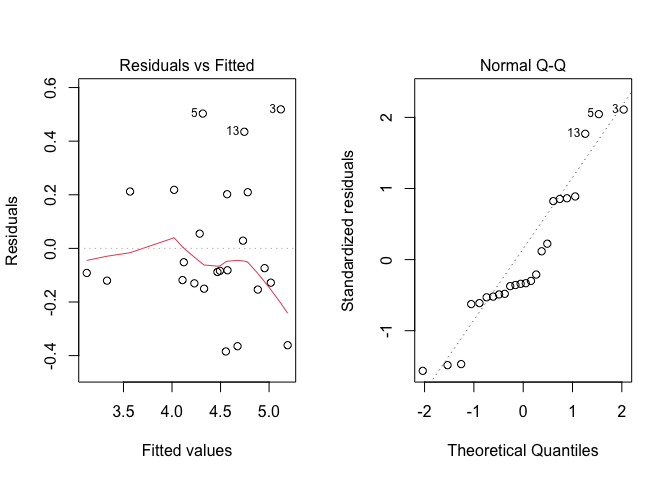
\includegraphics[width=0.9\linewidth]{_main_files/figure-latex/figName121-1} 

}

\caption{Analisi grafica dei residui per la prova di confronto erbicida}\label{fig:figName121}
\end{figure}

Dopo esserci rassicurati su questo importante aspetto, possiamo vedere che abbiamo due ipotesi nulle da testare (effetto del trattamento non significativo ed effetto del blocco non significativo), che possono essere entrambe rifiutate per P \textless{} 0.05.

Da questo punto in avanti, l'analisi procede come usuale, calcolando le medie marginali attese ed, eventualmente, confrontandole tra loro con una procedura di confronto multiplo, come descritto nei capitoli precedenti. Tener presente che, in questo esperimento, abbiamo 16 trattamenti, cioè \(16 \times 15 / 2 = 120\) confronti; di conseguenza, può essere opportuno operare la correzione per la molteplicità. Inoltre, dato che il trattamento più interessante è quello che rende massima la produzione, sarà opportuno ordinare le medie in senso decrescente, utilizzando l'argomento `reverse = T'.

\scriptsize

\begin{Shaded}
\begin{Highlighting}[]
\KeywordTok{library}\NormalTok{(emmeans)}
\NormalTok{medie <-}\StringTok{ }\KeywordTok{emmeans}\NormalTok{(mod, }\OperatorTok{~}\KeywordTok{factor}\NormalTok{(Herbicide))}
\NormalTok{multcomp}\OperatorTok{::}\KeywordTok{cld}\NormalTok{(medie, }\DataTypeTok{Letters =}\NormalTok{ LETTERS, }\DataTypeTok{reverse =}\NormalTok{ T)}
\CommentTok{##  Herbicide                                  emmean   SE df lower.CL upper.CL .group}
\CommentTok{##  Rimsulfuron (50)                             98.0 6.32 45    85.24    110.7  A    }
\CommentTok{##  Rimsulfuron + Atred                          97.0 6.32 45    84.26    109.7  A    }
\CommentTok{##  Pendimethalin (post) + rimsuulfuron (post)   96.6 6.32 45    83.91    109.4  A    }
\CommentTok{##  Rimsulfuron (40)                             95.4 6.32 45    82.67    108.1  A    }
\CommentTok{##  Rimsulfuron + hoeing                         93.9 6.32 45    81.18    106.6  A    }
\CommentTok{##  Rimsulfuron (45)                             91.6 6.32 45    78.84    104.3  A    }
\CommentTok{##  Rimsulfuron (50+30 split)                    89.2 6.32 45    76.52    102.0  A    }
\CommentTok{##  Hand-Weeded                                  89.0 6.32 45    76.24    101.7  A    }
\CommentTok{##  Rimsulfuron (60)                             88.4 6.32 45    75.65    101.1  A    }
\CommentTok{##  Rimsulfuron + thyfensulfuron                 84.7 6.32 45    71.94     97.4  A    }
\CommentTok{##  Pendimethalin (pre) + rimsulfuron (post)     83.0 6.32 45    70.31     95.8  AB   }
\CommentTok{##  Thifensulfuron                               51.9 6.32 45    39.19     64.6   BC  }
\CommentTok{##  Metolachlor + terbuthylazine (pre)           47.0 6.32 45    34.27     59.7    C  }
\CommentTok{##  Unweeded 2                                   35.7 6.32 45    22.99     48.4    C  }
\CommentTok{##  Alachlor + terbuthylazine                    29.8 6.32 45    17.11     42.6    C  }
\CommentTok{##  Unweeded 1                                   21.9 6.32 45     9.13     34.6    C  }
\CommentTok{## }
\CommentTok{## Results are averaged over the levels of: Block }
\CommentTok{## Confidence level used: 0.95 }
\CommentTok{## P value adjustment: tukey method for comparing a family of 16 estimates }
\CommentTok{## significance level used: alpha = 0.05}
\end{Highlighting}
\end{Shaded}

\normalsize

Vi lascio il commento dei risultati come esercizio.

\hypertarget{disegni-a-quadrato-latino-1}{%
\section{Disegni a quadrato latino}\label{disegni-a-quadrato-latino-1}}

A volte i fattori di blocco sono più di uno e danno origine ad un disegno sperimentale detto `quadrato latino' di cui abbiamo parlato nel capitolo 3. Qui, forniremo un esempio tratto dalla pratica sperimentale industriale.

\hypertarget{caso-studio-confronto-tra-metodi-costruttivi}{%
\section{Caso studio: confronto tra metodi costruttivi}\label{caso-studio-confronto-tra-metodi-costruttivi}}

Immaginiamo di voler studiare il tempo necessario per costruire un componente elettronico, utilizzando quattro metodi diversi. E' evidente che il tempo di costruzione sarà influenzato dalla perizia del tecnico e, per questo, utilizziamo quattro tecnici diversi, ad ognuno dei quali facciamo utilizzare tutti e quattro i metodi. Un esperimento così disegnato sarebbe a blocchi randomizzati, con il tecnico che fa da blocco per i trattamenti. Tuttavia, dobbiamo anche riconoscere che i quattro tecnici saranno via via meno efficienti, e quindi il metodo che utilizzeranno per primo sarà avvantaggiato, mentre quello che utilizzeranno per ultimo sarà svantaggiato. E'vero che i metodi sono assegnati in ordine random ad ogni tecnico, ma non si può comunque evitare che un metodo venga avvantaggiato rispetto ad un altro, perché, ad esempio, non viene mai ad occupare l'ultima posizione (o meglio, l'ultimo turno).

Per evitare questo problema imponiamo un vincolo ulteriore alla randizzazione e facciamo in modo che ogni metodo occupi tutte e quattro i turni, in tecnici diversi. Il disegno è quindi a quadrato latino.

Il dataset dei risultati è disponibile su gitHub:

\begin{Shaded}
\begin{Highlighting}[]
\NormalTok{path1 <-}\StringTok{ "https://raw.githubusercontent.com/OnofriAndreaPG/"}
\NormalTok{path2 <-}\StringTok{ "aomisc/master/data/"}
\NormalTok{fileName <-}\StringTok{ "Technicians.csv"}
\NormalTok{filePath <-}\StringTok{ }\KeywordTok{paste}\NormalTok{(path1, path2, fileName, }\DataTypeTok{sep =} \StringTok{""}\NormalTok{)}
\NormalTok{dataset <-}\StringTok{ }\KeywordTok{read.csv}\NormalTok{(filePath, }\DataTypeTok{header=}\NormalTok{T)}
\NormalTok{dataset}
\CommentTok{##    Shift Technician Method Time}
\CommentTok{## 1      I     Andrew      C   90}
\CommentTok{## 2     II     Andrew      B   90}
\CommentTok{## 3    III     Andrew      A   89}
\CommentTok{## 4     IV     Andrew      D  104}
\CommentTok{## 5      I       Anna      D   96}
\CommentTok{## 6     II       Anna      C   91}
\CommentTok{## 7    III       Anna      B   97}
\CommentTok{## 8     IV       Anna      A  100}
\CommentTok{## 9      I    Michael      A   84}
\CommentTok{## 10    II    Michael      D   96}
\CommentTok{## 11   III    Michael      C   98}
\CommentTok{## 12    IV    Michael      B  104}
\CommentTok{## 13     I      Sarah      B   88}
\CommentTok{## 14    II      Sarah      A   88}
\CommentTok{## 15   III      Sarah      D   98}
\CommentTok{## 16    IV      Sarah      C  106}
\end{Highlighting}
\end{Shaded}

\hypertarget{definizione-di-un-modello-lineare-2}{%
\section{Definizione di un modello lineare}\label{definizione-di-un-modello-lineare-2}}

In questo caso abbiamo un trattamento (metodo) e due effetti `blocco' (tecnico e turno) da includere nel modello, che può essere così definito:

\[Y_{ijk} = \mu + \gamma_k + \beta_j + \alpha_i + \varepsilon_{ijk}\]

dove \(\mu\) è l'intercetta, \(\gamma\) è l'effetto del turno k, \(\beta\) è l'effetto del tecnico j e \(\alpha\) è l'effetto del metodo i. L'elemento \(\varepsilon_{ijk}\) rappresenta la componente random individuale, di ogni osservazione e si assume normalmente distribuita, con media 0 e deviazione standard \(\sigma\).

Avendo già illustrato il processo di stima dei parametri e di scomposizione della varianza e quindi utilizziamo subito R per il `model fitting':

\begin{Shaded}
\begin{Highlighting}[]
\NormalTok{mod <-}\StringTok{ }\KeywordTok{lm}\NormalTok{(Time }\OperatorTok{~}\StringTok{ }\NormalTok{Method }\OperatorTok{+}\StringTok{ }\NormalTok{Technician}
          \OperatorTok{+}\StringTok{ }\NormalTok{Shift, }\DataTypeTok{data =}\NormalTok{ dataset)}
\end{Highlighting}
\end{Shaded}

Verifichiamo il rispetto delle assunzioni di base, con l'analisi grafica dei residui, riportata in Figura \ref{fig:figName122} (il codice è analogo a quello fornito più sopra).

\begin{figure}

{\centering 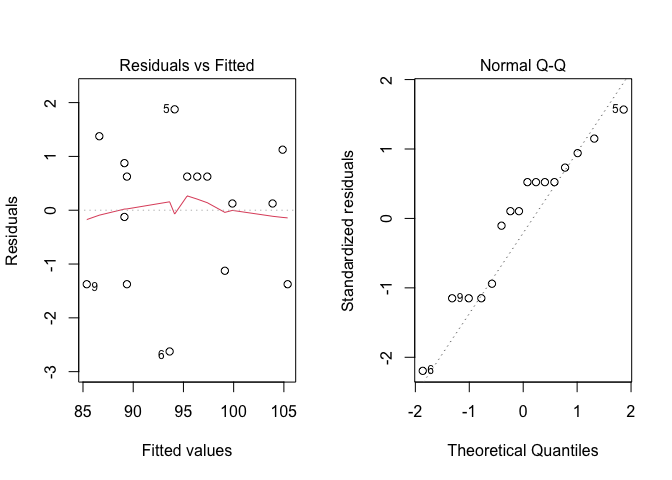
\includegraphics[width=0.9\linewidth]{_main_files/figure-latex/figName122-1} 

}

\caption{Analisi grafica dei residui per la prova di confronto tra metodi costruttivi}\label{fig:figName122}
\end{figure}

Non essendovi evidenti problemi, valutiamo la significatività degli effetti nel modello, analogamente a quanto abbiamo fatto nel caso dell'ANOVA a blocchi randomizzati. L'unica differenza sta nel fatto che, nei disegni a quadrato latino, vi sono tre effetti da testare, anche se l'unico ad avere una certa rilevanza è l'effetto del metodo di lavoro.

\begin{Shaded}
\begin{Highlighting}[]
\KeywordTok{anova}\NormalTok{(mod)}
\CommentTok{## Analysis of Variance Table}
\CommentTok{## }
\CommentTok{## Response: Time}
\CommentTok{##            Df Sum Sq Mean Sq F value    Pr(>F)    }
\CommentTok{## Method      3 145.69  48.563 12.7377 0.0051808 ** }
\CommentTok{## Technician  3  17.19   5.729  1.5027 0.3065491    }
\CommentTok{## Shift       3 467.19 155.729 40.8470 0.0002185 ***}
\CommentTok{## Residuals   6  22.87   3.812                      }
\CommentTok{## ---}
\CommentTok{## Signif. codes:  0 '***' 0.001 '**' 0.01 '*' 0.05 '.' 0.1 ' ' 1}
\end{Highlighting}
\end{Shaded}

Vediamo che esiste una differenza significativa tra i metodi e l'ipotesi nulla può essere rifiutata con una bassissima probabilità di errore di prima specie.

Ovviamente, dopo aver eseguito un'ANOVA a blocchi randomizzati o a quadrato latino, andremo eventualmente ad eseguire un test di confronto multiplo, seguendo le raccomandazioni esposte nel capitolo precedente. Anche questa parte ve la lascio per esercizio.

\hypertarget{modelli-anova-a-due-vie}{%
\chapter{Modelli ANOVA a due vie}\label{modelli-anova-a-due-vie}}

\hypertarget{il-concetto-di-interazione}{%
\section{Il concetto di 'interazione'}\label{il-concetto-di-interazione}}

In alcuni casi potremmo essere interessati ad organizzare un esperimento per valutare l'effetto di due fattori sperimentali combinati (ad esempio la lavorazione del terreno ed il diserbo chimico), in modo da mettere in evidenza possibili ``interazioni''. Con questo termine intendiamo il fenomeno per cui l'effetto di un fattore (ad es. la lavorazione) cambia a seconda del livello dell'altro fattore (il diserbo chimico). Ad esempio, nella Tabella \ref{tab:tabName131}, A2 da un risultato più elevato di A1, quando il secondo fattore sperimentale è B1, mentre la graduatoria è invertita con B2.

\begin{table}[t]

\caption{\label{tab:tabName131}Interazione tra due fattori sperimentali}
\centering
\begin{tabular}{lccc}
\toprule
  & B1 & B2 & Media\\
\midrule
A1 & 10 & 17.0 & 13.5\\
A2 & 14 & 6.0 & 10.0\\
Media & 12 & 11.5 & 11.8\\
\bottomrule
\end{tabular}
\end{table}

In termini algebrici, l'interazione può essere calcolata come mancanza di additività. Se guardiamo la tabella sovrastante, osserviamo che il trattamento A1 ha incrementato il risultato di 1.75 unità rispetto alla media generale, mentre il trattamento B1 ha incrementato il risultato di 0.25 unità, sempre rispetto alla media generale. Di conseguenza, per la combinazione A1B1 ci aspetteremmo un risultato finale additivo, pari a 11.75 + 1.75 + 0.25 = 13.75, mentre il risultato finale è di 10 unità. Evidentemente la combinazione A1B1 è una combinazione svantaggiosa, cioè i due trattamenti interagiscono tra di loro in modo negativo, portando ad un risultato inferiore alle attese.

La presenza di interazione può influenzare notevolmente l'interpretazione dei risultati. Infatti, tornadno alla Tabella \ref{tab:tabName131}, se guardassimo solo alle medie marginali del fattore A, saremmo portati a concludere che i due livelli A1 ed A2 forniscono, più o meno, gli stessi risultati. In realtà questo è falso, in quanto A1 ed A2 forniscono risultati molto diversi, ma le differenze sono di segno opposto, a seconda del livello di B.

\hypertarget{tipi-di-interazione}{%
\section{Tipi di interazione}\label{tipi-di-interazione}}

In genere, abbiamo due tipi di interazione: quella in cui cambia la graduatoria tra i trattamenti (interazione crossover) e quella in cui vi è solo una modifica dell'entità dell'effetto (interazione semplice o non-crossover). I due tipi di interazione sono esemplificati in Figura \ref{fig:figName131}. Da un punto di vista dell'interpretazione dei risultati, l'interazione cross-over è particolarmente importante, perché non consente di raggiungere conclusioni generali per i due fattori sperimentali presi indipendentemente l'uno dall'altro.

\begin{figure}

{\centering 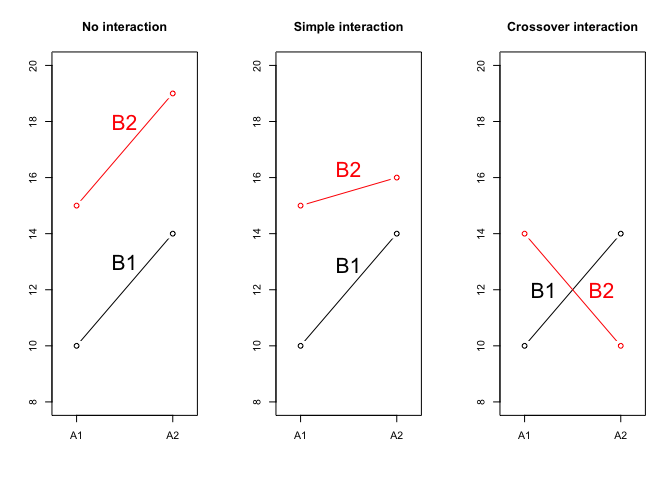
\includegraphics[width=0.9\linewidth]{_main_files/figure-latex/figName131-1} 

}

\caption{Esempi di interazione tra fattori sperimentali}\label{fig:figName131}
\end{figure}

\hypertarget{caso-studio-interazione-tra-lavorazioni-e-diserbo-chimico}{%
\section{Caso-studio: interazione tra lavorazioni e diserbo chimico}\label{caso-studio-interazione-tra-lavorazioni-e-diserbo-chimico}}

Un ricercatore ha organizzato un esperimento fattoriale a blocchi randomizzati, dove ha valutato l'effetto di tre tipi di lavorazione del terreno (lavorazione minima = MIN; aratura superficiale = SUP; aratura profonda = PROF) e di due tipi di diserbo chimico (a pieno campo = TOT; localizzato sulla fila della coltura = PARZ). L'ipotesi scientifica è che, in caso di diserbo localizzato, il rovesciamento del terreno prodotto dall'aratura sia fondamentale, in quanto sotterra i semi prodotti dalle piante infestanti, impedendone l'emergenza nella coltura successiva e rendendo quindi necessario il diserbo a tutta superficie. La mappa di campo è presentata in Figura \ref{fig:figName132}; dobbiamo notare lo spazio lasciato tra una parcella e l'altra, per permettere l'uso e la circolazione delle macchine per la lavorazione.

\begin{figure}

{\centering 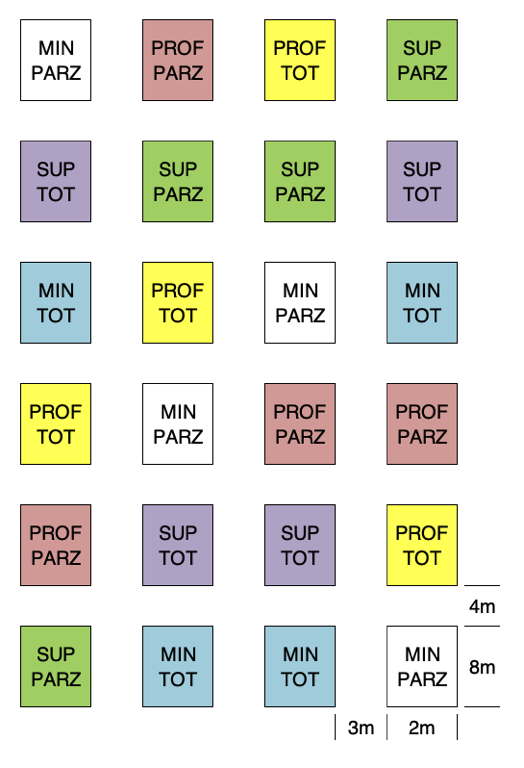
\includegraphics[width=0.45\linewidth]{_images/Mappa3FATT} 

}

\caption{Mappa dell'esperimento fattoriale a blocchi randomizzati}\label{fig:figName132}
\end{figure}

In totale, l'esperimento include sei tesi (le sei possibili combinazioni tra i due fattori sperimentali) e quattro repliche per un totale di 24 parcelle. Come consuetudine in pieno campo, l'esperimento è organizzato a blocchi randomizzati e le sei tesi sperimentali sono allocate a caso all'interno di ciascun blocco.

I risultati ottenuti con questo esperimento sono disponibili nel file `beet.csv', che può essere aperto direttamente da gitHub, con il codice sottostante.

\begin{Shaded}
\begin{Highlighting}[]
\NormalTok{path1 <-}\StringTok{ "https://raw.githubusercontent.com/OnofriAndreaPG/"}
\NormalTok{path2 <-}\StringTok{ "aomisc/master/data/"}
\NormalTok{name <-}\StringTok{ "beet.csv"}
\NormalTok{pathName <-}\StringTok{ }\KeywordTok{paste}\NormalTok{(path1, path2, name, }\DataTypeTok{sep =} \StringTok{""}\NormalTok{)}
\NormalTok{dataset <-}\StringTok{ }\KeywordTok{read.csv}\NormalTok{(pathName, }\DataTypeTok{header=}\NormalTok{T)}
\KeywordTok{head}\NormalTok{(dataset)}
\CommentTok{##   Lavorazione Diserbo Blocco   Prod}
\CommentTok{## 1         MIN     tot      1 11.614}
\CommentTok{## 2         MIN     tot      2  9.283}
\CommentTok{## 3         MIN     tot      3  7.019}
\CommentTok{## 4         MIN     tot      4  8.015}
\CommentTok{## 5         MIN    parz      1  5.117}
\CommentTok{## 6         MIN    parz      2  4.306}
\end{Highlighting}
\end{Shaded}

\hypertarget{definizione-del-modello-lineare}{%
\section{Definizione del modello lineare}\label{definizione-del-modello-lineare}}

I risultati di questo esperimento sono determinati da quattro elementi `deterministici':

\begin{enumerate}
\def\labelenumi{\arabic{enumi}.}
\tightlist
\item
  l'effetto del blocco
\item
  l'effetto della lavorazione
\item
  l'effetto del diserbo chimico
\item
  l'interazione `lavorazione \(\times\) diserbo'
\end{enumerate}

Un modello lineare con questi quattro effetti potrebbe essere scritto:

\[Y_{ijk} = \mu + \gamma_k + \alpha_i + \beta_j + \alpha\beta_{ij} + \varepsilon_{ijk}\]

dove \(\gamma\) è l'effetto del blocco \(k\), \(\alpha\) è l'effetto della lavorazione \(i\), \(\beta\) è l'effetto del diserbo \(j\), \(\alpha\beta\) è l'effetto dell'interazione per la specifica combinazione della lavorazione \(i\) e del diserbo \(j\). Oltre a questi elementi `deterministici' i risultati sono influenzati dall'elemento stocastico \(\varepsilon\), associato ad ogni osservazione, che si assume normalmente distribuito con media 0 e deviazione standard pari a \(\sigma\).

\hypertarget{stima-dei-parametri-2}{%
\section{Stima dei parametri}\label{stima-dei-parametri-2}}

Per rendere `stimabili' i parametri, poniamo un vincolo sul trattamento, per cui \(\gamma_1 = 0\), \(\alpha_1 = 0\) (primo livello in ordine alfabetico, cioè MIN), \(\beta_1 = 0\) (primo livello in ordine alfabetico, cioè PARZ). Per quanto riguarda l'interazione \(\alpha\beta\), abbiamo 6 combinazioni possibili tra il primo e il secondo fattore (MIN - TOT, MIN - PARZ, SUP - TOT, SUP - PARZ, PROF - TOT, PROF - PARZ); di queste, dobbiamo vincolare tutte le combinazioni che contengono il primo livello in ordine alfabetico per uno dei due fattori (MIN - TOT, MIN - PARZ, SUP - PARZ, PROF - PARZ, corrispondenti ad \(\alpha\beta_{1,1}\) = \(\alpha\beta_{1,2}\) = \(\alpha\beta_{2,1}\) = \(\alpha\beta_{3,1}\) = 0).

Con questi vincoli, \(\mu\) è il valore atteso per la parcella localizzata nel primo blocco e trattata con il primo livello in ordine alfabetico per tutti i fattori sperimentali (\(\bar{Y}_{111}\)). I tre valori \(\gamma\) rappresentano rispettivamente \(\gamma_2 = \bar{Y}_{112} - \bar{Y}_{111}\), \(\gamma_3 = \bar{Y}_{113} - \bar{Y}_{111}\) e \(\gamma_4 = \bar{Y}_{114} - \bar{Y}_{111}\). Abbiamo invece che \(\alpha_2 = \bar{Y}_{211} - \bar{Y}_{111}\) e \(\alpha_3 = \bar{Y}_{311} - \bar{Y}_{111}\), mentre \(\beta_2 = \bar{Y}_{121} - \bar{Y}_{111}\) e \(\beta_3 = \bar{Y}_{131} - \bar{Y}_{111}\). Per quanto riguarda l'interazione, abbiamo due soli parametri da stimare, per i quali possiamo fare le seguenti considerazioni:

\[\bar{Y}_{111} = \mu + \alpha_1 + \beta_1 + \alpha\beta_{11} = \mu\]

\[\bar{Y}_{221} = \mu + \alpha_2 + \beta_2 + \alpha\beta_{22}\]

quindi:

\[\bar{Y}_{221} - \bar{Y}_{111} = \alpha_2 + \beta_2 + \alpha\beta_{22}\]

da cui:

\[\alpha\beta_{22} = \bar{Y}_{221} - \bar{Y}_{111} - \alpha_2 - \beta_2\]

Analogamente:

\[\alpha\beta_{32} = \bar{Y}_{321} - \bar{Y}_{111} - \alpha_3 - \beta_2\]

Vediamo che, quando i modelli divengono appena appena più complessi, la parametrizzazione con vincolo sulla somma diventa abbastanza controintuitiva, e, inoltre, la stima dei parametri diventa abbastanza difficile da fare a mano. Al contrario, quest'operazione è piuttosto semplice e intuitiva quando si impieghi il vincolo sulla somma. Per chi volesse approfondire, ci sono alcune ulteriori informazioni in fondo al capitolo.

In questa sede, per la stima dei parametri ci affidiamo ad R e al metodo dei minimi quadrati, confidando che le informazioni precedenti possano essere utili a capire l'output del programma.

\footnotesize

\begin{Shaded}
\begin{Highlighting}[]
\NormalTok{mod <-}\StringTok{ }\KeywordTok{lm}\NormalTok{(Prod }\OperatorTok{~}\StringTok{ }\KeywordTok{factor}\NormalTok{(Blocco) }\OperatorTok{+}\StringTok{ }\NormalTok{Lavorazione }\OperatorTok{+}\StringTok{ }\NormalTok{Diserbo }\OperatorTok{+}
\StringTok{            }\NormalTok{Lavorazione}\OperatorTok{:}\NormalTok{Diserbo, }\DataTypeTok{data=}\NormalTok{dataset)}
\KeywordTok{summary}\NormalTok{(mod)}
\CommentTok{## }
\CommentTok{## Call:}
\CommentTok{## lm(formula = Prod ~ factor(Blocco) + Lavorazione + Diserbo + }
\CommentTok{##     Lavorazione:Diserbo, data = dataset)}
\CommentTok{## }
\CommentTok{## Residuals:}
\CommentTok{##      Min       1Q   Median       3Q      Max }
\CommentTok{## -1.78329 -0.78754 -0.04437  0.31117  3.12546 }
\CommentTok{## }
\CommentTok{## Coefficients:}
\CommentTok{##                            Estimate Std. Error t value Pr(>|t|)    }
\CommentTok{## (Intercept)                  6.6422     0.8376   7.930 9.59e-07 ***}
\CommentTok{## factor(Blocco)2             -1.0380     0.7897  -1.314 0.208431    }
\CommentTok{## factor(Blocco)3             -0.8277     0.7897  -1.048 0.311179    }
\CommentTok{## factor(Blocco)4             -0.7232     0.7897  -0.916 0.374267    }
\CommentTok{## LavorazionePROF              4.6338     0.9671   4.791 0.000238 ***}
\CommentTok{## LavorazioneSUP               2.4803     0.9671   2.565 0.021568 *  }
\CommentTok{## Diserbotot                   2.9878     0.9671   3.089 0.007480 ** }
\CommentTok{## LavorazionePROF:Diserbotot  -4.4098     1.3677  -3.224 0.005677 ** }
\CommentTok{## LavorazioneSUP:Diserbotot   -2.3218     1.3677  -1.698 0.110246    }
\CommentTok{## ---}
\CommentTok{## Signif. codes:  0 '***' 0.001 '**' 0.01 '*' 0.05 '.' 0.1 ' ' 1}
\CommentTok{## }
\CommentTok{## Residual standard error: 1.368 on 15 degrees of freedom}
\CommentTok{## Multiple R-squared:  0.641,  Adjusted R-squared:  0.4495 }
\CommentTok{## F-statistic: 3.348 on 8 and 15 DF,  p-value: 0.02095}
\end{Highlighting}
\end{Shaded}

\normalsize

Una volta stimati i parametri, possiamo individuare la devianza residua, come somma dei quadrati degli scarti tra i valori attesi e i valori osservati. I residui, in R, possono essere ottenuti con la funzione `residuals()'.

\begin{Shaded}
\begin{Highlighting}[]
\NormalTok{RSS <-}\StringTok{ }\KeywordTok{sum}\NormalTok{( }\KeywordTok{residuals}\NormalTok{(mod)}\OperatorTok{^}\DecValTok{2}\NormalTok{ )}
\NormalTok{RSS}
\CommentTok{## [1] 28.06087}
\end{Highlighting}
\end{Shaded}

Consideriamo che la devianza del residuo ha un numero di gradi di libertà pari alla differenza tra il numero dei dati è il numero dei parametri stimati (24 - 9 = 15). Di conseguenza, possiamo stimare \(\sigma\), come:

\begin{Shaded}
\begin{Highlighting}[]
\KeywordTok{sqrt}\NormalTok{(RSS}\OperatorTok{/}\DecValTok{15}\NormalTok{)}
\CommentTok{## [1] 1.367744}
\end{Highlighting}
\end{Shaded}

o, più velocemente, con l'apposito estrattore:

\begin{Shaded}
\begin{Highlighting}[]
\KeywordTok{summary}\NormalTok{(mod)}\OperatorTok{$}\NormalTok{sigma}
\CommentTok{## [1] 1.367744}
\end{Highlighting}
\end{Shaded}

\hypertarget{verifica-delle-assunzioni-di-base}{%
\section{Verifica delle assunzioni di base}\label{verifica-delle-assunzioni-di-base}}

Dobbiamo quindi procedere con la verifica delle assunzioni di base, attraverso l'analisi grafica dei residui, come indicato in un capitolo precedente. Il grafico dei residui contro i valori attesi ed il QQ-plot sono riportati in Figura \ref{fig:figName133}.

\begin{figure}

{\centering 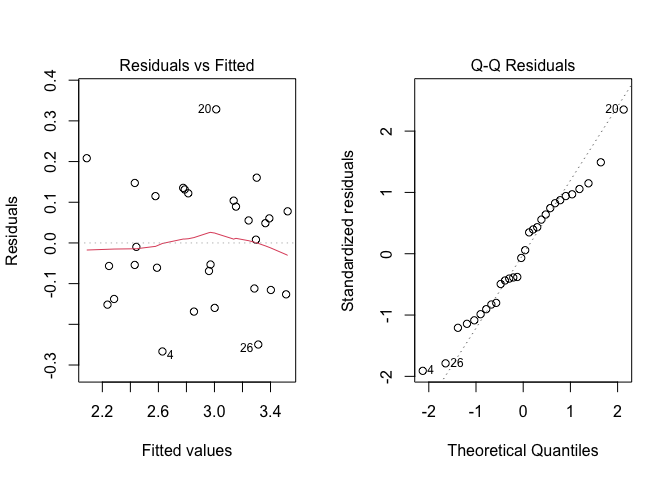
\includegraphics[width=0.9\linewidth]{_main_files/figure-latex/figName133-1} 

}

\caption{Analisi grafica dei residui con R}\label{fig:figName133}
\end{figure}

Il grafico dei residui mostra un sospetto outlier (il settimo dato). Tuttavia, non abbiamo memoria di errori durante la sperimentazione e a parte questo outlier, non paiono esserci problemi di omogeneità delle varianze. Pertanto, decidiamo di ignorare questo potenziale dato aberrante e proseguire nell'analisi, in quanto non sussistono particolare elementi che facciano sospettare qualche patologia dei dati più o meno rilevante.

\hypertarget{scomposizione-delle-varianze}{%
\section{Scomposizione delle varianze}\label{scomposizione-delle-varianze}}

Se dovessimo scomporre le varianze manualmente, potremmo costruire il modello in modo sequenziale, il che è totalmente corretto con i disegni bilanciati come il nostro.

\begin{Shaded}
\begin{Highlighting}[]
\NormalTok{mod0 <-}\StringTok{ }\KeywordTok{lm}\NormalTok{(Prod }\OperatorTok{~}\StringTok{ }\DecValTok{1}\NormalTok{, }\DataTypeTok{data=}\NormalTok{dataset)}
\NormalTok{mod1 <-}\StringTok{ }\KeywordTok{lm}\NormalTok{(Prod }\OperatorTok{~}\StringTok{ }\KeywordTok{factor}\NormalTok{(Blocco), }\DataTypeTok{data=}\NormalTok{dataset)}
\NormalTok{mod2 <-}\StringTok{ }\KeywordTok{lm}\NormalTok{(Prod }\OperatorTok{~}\StringTok{ }\KeywordTok{factor}\NormalTok{(Blocco) }\OperatorTok{+}\StringTok{ }\NormalTok{Lavorazione, }\DataTypeTok{data=}\NormalTok{dataset)}
\NormalTok{mod3 <-}\StringTok{ }\KeywordTok{lm}\NormalTok{(Prod }\OperatorTok{~}\StringTok{ }\KeywordTok{factor}\NormalTok{(Blocco) }\OperatorTok{+}\StringTok{ }\NormalTok{Lavorazione }\OperatorTok{+}\StringTok{ }\NormalTok{Diserbo, }
            \DataTypeTok{data=}\NormalTok{dataset)}
\NormalTok{mod4 <-}\StringTok{ }\KeywordTok{lm}\NormalTok{(Prod }\OperatorTok{~}\StringTok{ }\KeywordTok{factor}\NormalTok{(Blocco) }\OperatorTok{+}\StringTok{ }\NormalTok{Lavorazione }\OperatorTok{+}\StringTok{ }\NormalTok{Diserbo }\OperatorTok{+}
\StringTok{            }\NormalTok{Lavorazione}\OperatorTok{:}\NormalTok{Diserbo, }\DataTypeTok{data=}\NormalTok{dataset)}
\NormalTok{RSS0 <-}\StringTok{ }\KeywordTok{deviance}\NormalTok{(mod0)}
\NormalTok{RSS1 <-}\StringTok{ }\KeywordTok{deviance}\NormalTok{(mod1)}
\NormalTok{RSS2 <-}\StringTok{ }\KeywordTok{deviance}\NormalTok{(mod2)}
\NormalTok{RSS3 <-}\StringTok{ }\KeywordTok{deviance}\NormalTok{(mod3)}
\NormalTok{RSS4 <-}\StringTok{ }\KeywordTok{deviance}\NormalTok{(mod4)}
\end{Highlighting}
\end{Shaded}

Vediamo che il modello nullo ha un residuo pari a 78.161505, mentre il il modello con il solo effetto del blocco ha un residuo più basso e pari 74.5019152. Evidentemente, l'introduzione del blocco ha migliorato la capacità descrittiva del modello e l'effetto di questa variabile può essere quantificato con la differenza tra le due devianze:

\begin{Shaded}
\begin{Highlighting}[]
\NormalTok{RSS0 }\OperatorTok{-}\StringTok{ }\NormalTok{RSS1}
\CommentTok{## [1] 3.65959}
\end{Highlighting}
\end{Shaded}

Analogamente, l'effetto della lavorazione (devianza della lavorazione) è dato da:

\begin{Shaded}
\begin{Highlighting}[]
\NormalTok{RSS1 }\OperatorTok{-}\StringTok{ }\NormalTok{RSS2}
\CommentTok{## [1] 23.65647}
\end{Highlighting}
\end{Shaded}

Ovviamente, possiamo evitare di procedere in questo modo, sfruttando le funzionalità di R e, in particolare, la funzione `anova()':

\footnotesize

\begin{Shaded}
\begin{Highlighting}[]
\KeywordTok{anova}\NormalTok{(mod)}
\CommentTok{## Analysis of Variance Table}
\CommentTok{## }
\CommentTok{## Response: Prod}
\CommentTok{##                     Df  Sum Sq Mean Sq F value  Pr(>F)  }
\CommentTok{## factor(Blocco)       3  3.6596  1.2199  0.6521 0.59389  }
\CommentTok{## Lavorazione          2 23.6565 11.8282  6.3228 0.01020 *}
\CommentTok{## Diserbo              1  3.3205  3.3205  1.7750 0.20266  }
\CommentTok{## Lavorazione:Diserbo  2 19.4641  9.7321  5.2023 0.01922 *}
\CommentTok{## Residuals           15 28.0609  1.8707                  }
\CommentTok{## ---}
\CommentTok{## Signif. codes:  0 '***' 0.001 '**' 0.01 '*' 0.05 '.' 0.1 ' ' 1}
\end{Highlighting}
\end{Shaded}

\normalsize

La quantificazione dei gradi di libertà dovrebbe essere chiara; aggiungiamo solo che, in generale, i gradi di libertà di un'interazione sono pari al prodotto tra i gradi di libertà degli effetti da cui essa è composta e coincidono con il numero di parametri stimati (in questo caso due).

Nel leggere una tabella ANOVA a due (o più) vie, è \textbf{fondamentale procedere dal basso verso l'alto}, in quanto la presenza di un'interazione significativa rende non-informative sia le significanze degli effetti principali, sia le medie marginali. Infatti, come abbiamo visto all'inizio, vi possono essere casi in cui le medie marginali sono simili, ma ciò è dovuto alla presenza di un'interazione cross-over. In questo caso, essendo significativa l'interazione tra lavorazione e diserbo, dovremo considerare e confrontare le sei medie per le combinazioni tra questi due fattori sperimentali.

\hypertarget{medie-marginali-attese-1}{%
\section{Medie marginali attese}\label{medie-marginali-attese-1}}

Può essere interessante vedere come si costruiscono le medie marginale attese, con un attento uso dei contrasti. Ad esempio, le medie attese per le sei combinazioni `lavorazione x diserbo' possono essere ottenute considerando che \(\mu\) è il valore atteso per MIN-PARZ nel primo blocco, mentre \(\mu + \gamma_2\) è il valore atteso per MIN-PARZ nel secondo blocco, e così via. Di conseguenza, la media per la combinazione MIN-PARZ sarà pari a:

\[ \frac{\mu + (\mu + \gamma_2) + (\mu + \gamma_3) + (\mu + \gamma_4)}{4} = \mu + \frac{1}{4}\gamma_2 + \frac{1}{4}\gamma_3 + \frac{1}{4}\gamma_4\]

I parametri stimati sono derivabili con la funzione `coef()', quindi la combinazione lineare sopra indicata può essere ottenuta come segue:

\begin{Shaded}
\begin{Highlighting}[]
\KeywordTok{coef}\NormalTok{(mod)[}\DecValTok{1}\NormalTok{] }\OperatorTok{+}\StringTok{ }\DecValTok{1}\OperatorTok{/}\DecValTok{4}\OperatorTok{*}\KeywordTok{coef}\NormalTok{(mod)[}\DecValTok{2}\NormalTok{] }\OperatorTok{+}\StringTok{ }\DecValTok{1}\OperatorTok{/}\DecValTok{4}\OperatorTok{*}\KeywordTok{coef}\NormalTok{(mod)[}\DecValTok{3}\NormalTok{] }\OperatorTok{+}\StringTok{ }\DecValTok{1}\OperatorTok{/}\DecValTok{4}\OperatorTok{*}\KeywordTok{coef}\NormalTok{(mod)[}\DecValTok{4}\NormalTok{]}
\CommentTok{## (Intercept) }
\CommentTok{##       5.995}
\end{Highlighting}
\end{Shaded}

Ovviamente, è più conveniente costruire una vettore con i coefficienti del contrasto, e moltiplicare per il vettore dei parametri stimati, come segue:

\begin{Shaded}
\begin{Highlighting}[]
\NormalTok{k1 <-}\StringTok{ }\KeywordTok{c}\NormalTok{(}\DecValTok{1}\NormalTok{, }\DecValTok{1}\OperatorTok{/}\DecValTok{4}\NormalTok{, }\DecValTok{1}\OperatorTok{/}\DecValTok{4}\NormalTok{, }\DecValTok{1}\OperatorTok{/}\DecValTok{4}\NormalTok{, }\DecValTok{0}\NormalTok{, }\DecValTok{0}\NormalTok{, }\DecValTok{0}\NormalTok{, }\DecValTok{0}\NormalTok{, }\DecValTok{0}\NormalTok{)}
\KeywordTok{sum}\NormalTok{( }\KeywordTok{coef}\NormalTok{(mod) }\OperatorTok{*}\StringTok{ }\NormalTok{k1 )}
\CommentTok{## [1] 5.995}
\end{Highlighting}
\end{Shaded}

Le altre medie, possono essere ottenute analogamente.

\begin{Shaded}
\begin{Highlighting}[]
\NormalTok{k2 <-}\StringTok{ }\KeywordTok{c}\NormalTok{(}\DecValTok{1}\NormalTok{, }\DecValTok{1}\OperatorTok{/}\DecValTok{4}\NormalTok{, }\DecValTok{1}\OperatorTok{/}\DecValTok{4}\NormalTok{, }\DecValTok{1}\OperatorTok{/}\DecValTok{4}\NormalTok{, }\DecValTok{1}\NormalTok{, }\DecValTok{0}\NormalTok{, }\DecValTok{0}\NormalTok{, }\DecValTok{0}\NormalTok{, }\DecValTok{0}\NormalTok{) }\CommentTok{#PROF - PARZ}
\NormalTok{k3 <-}\StringTok{ }\KeywordTok{c}\NormalTok{(}\DecValTok{1}\NormalTok{, }\DecValTok{1}\OperatorTok{/}\DecValTok{4}\NormalTok{, }\DecValTok{1}\OperatorTok{/}\DecValTok{4}\NormalTok{, }\DecValTok{1}\OperatorTok{/}\DecValTok{4}\NormalTok{, }\DecValTok{0}\NormalTok{, }\DecValTok{1}\NormalTok{, }\DecValTok{0}\NormalTok{, }\DecValTok{0}\NormalTok{, }\DecValTok{0}\NormalTok{) }\CommentTok{#SUP - PARZ}
\NormalTok{k4 <-}\StringTok{ }\KeywordTok{c}\NormalTok{(}\DecValTok{1}\NormalTok{, }\DecValTok{1}\OperatorTok{/}\DecValTok{4}\NormalTok{, }\DecValTok{1}\OperatorTok{/}\DecValTok{4}\NormalTok{, }\DecValTok{1}\OperatorTok{/}\DecValTok{4}\NormalTok{, }\DecValTok{0}\NormalTok{, }\DecValTok{0}\NormalTok{, }\DecValTok{1}\NormalTok{, }\DecValTok{0}\NormalTok{, }\DecValTok{0}\NormalTok{) }\CommentTok{#MIN - TOT}
\NormalTok{k5 <-}\StringTok{ }\KeywordTok{c}\NormalTok{(}\DecValTok{1}\NormalTok{, }\DecValTok{1}\OperatorTok{/}\DecValTok{4}\NormalTok{, }\DecValTok{1}\OperatorTok{/}\DecValTok{4}\NormalTok{, }\DecValTok{1}\OperatorTok{/}\DecValTok{4}\NormalTok{, }\DecValTok{1}\NormalTok{, }\DecValTok{0}\NormalTok{, }\DecValTok{1}\NormalTok{, }\DecValTok{1}\NormalTok{, }\DecValTok{0}\NormalTok{) }\CommentTok{#PROF - TOT}
\NormalTok{k6 <-}\StringTok{ }\KeywordTok{c}\NormalTok{(}\DecValTok{1}\NormalTok{, }\DecValTok{1}\OperatorTok{/}\DecValTok{4}\NormalTok{, }\DecValTok{1}\OperatorTok{/}\DecValTok{4}\NormalTok{, }\DecValTok{1}\OperatorTok{/}\DecValTok{4}\NormalTok{, }\DecValTok{0}\NormalTok{, }\DecValTok{1}\NormalTok{, }\DecValTok{1}\NormalTok{, }\DecValTok{0}\NormalTok{, }\DecValTok{1}\NormalTok{) }\CommentTok{#SUP - TOT}
\KeywordTok{sum}\NormalTok{( }\KeywordTok{coef}\NormalTok{(mod) }\OperatorTok{*}\StringTok{ }\NormalTok{k2 )}
\CommentTok{## [1] 10.62875}
\KeywordTok{sum}\NormalTok{( }\KeywordTok{coef}\NormalTok{(mod) }\OperatorTok{*}\StringTok{ }\NormalTok{k3 )}
\CommentTok{## [1] 8.47525}
\KeywordTok{sum}\NormalTok{( }\KeywordTok{coef}\NormalTok{(mod) }\OperatorTok{*}\StringTok{ }\NormalTok{k4 )}
\CommentTok{## [1] 8.98275}
\KeywordTok{sum}\NormalTok{( }\KeywordTok{coef}\NormalTok{(mod) }\OperatorTok{*}\StringTok{ }\NormalTok{k5 )}
\CommentTok{## [1] 9.20675}
\KeywordTok{sum}\NormalTok{( }\KeywordTok{coef}\NormalTok{(mod) }\OperatorTok{*}\StringTok{ }\NormalTok{k6 )}
\CommentTok{## [1] 9.14125}
\end{Highlighting}
\end{Shaded}

Anche se è comodo conoscere come eseguire queste operazioni, da un punto di vista pratico è certamente più comodo utilizzare la funzione `emmeans()' del package `emmeans', di cui daremo un esempio tra poco.

\hypertarget{calcolo-degli-errori-standard-sem-e-sed}{%
\section{Calcolo degli errori standard (SEM e SED)}\label{calcolo-degli-errori-standard-sem-e-sed}}

Tutte le quantità ottenute più sopra sono state calcolate come combinazioni lineari di parametri del modello. Di conseguenza, le loro varianze sono derivabili con la legge di propagazione degli errori. In questo caso semplice (dati bilanciati), possiamo utilizzare la usuale formula per la quale l'errore standard di una media si ottiene dalla radice quadrata del rapporto tra la varianza del residuo e il numero delle repliche.

Tuttavia, anche se la varianza del residuo è la stessa, il numero di dati che concorrono a formare le medie è diverso (diverso numero di repliche). Infatti, le medie di ogni combinazione `diserbo x lavorazione' hanno un numero di repliche pari a quattro, mentre le lavorazioni hanno un numero di repliche pari a quattro per il numero dei livelli di diserbo (cioè 8). Il diserbo ha invece un numero di repliche pari a quattro per il numero dei livelli di lavorazione (cioè 12).

Di conseguenza:

\[SEM_A = \sqrt{\frac{1.87}{4 \cdot 2}} = 0.483\]

\[SEM_B = \sqrt{\frac{1.87}{4 \cdot 3}} = 0.395\]

\[SEM_{AB} = \sqrt{\frac{1.87}{4}} = 0.684\]

Possiamo notare che le medie degli effetti principali, grazie al numero di repliche più elevato, sono stimate con maggiore precisione delle medie delle combinazioni.

Per quanto riguarda gli errori standard delle differenze tra medie (SED), questi si ottengono dai SEM, moltiplicandoli per \(\sqrt(2)\), come usuale. Dai SED, posso calcolare le Minime Differenze Significative, moltiplicandoli per il valore di t di Student, per il 5\% di probabilità (test a due code) e 15 gradi di libertà, pari a 2.131.

Dato che l'interazione è significativa, posso fare i confronti multipli solo tra le medie delle combinazioni `diserbo x lavorazione', dato che confrontare le medie degli effetti principali potrebbe portare a risultati poco attendibili, per i motivi precedentemente esposti.

\hypertarget{medie-marginali-attese-e-confronti-multipli-con-r}{%
\section{Medie marginali attese e confronti multipli con R}\label{medie-marginali-attese-e-confronti-multipli-con-r}}

Per ottenere medie, confronti multipli o altre analisi routinarie, possiamo utilizzare il package `emmeans'. Il codice sottostante calcola le medie per le combinazioni `lavorazione x diserbo' e confronta i diserbi a parità di lavorazione.

\begin{Shaded}
\begin{Highlighting}[]
\KeywordTok{library}\NormalTok{(emmeans)}
\NormalTok{medie <-}\StringTok{ }\KeywordTok{emmeans}\NormalTok{(mod, }\OperatorTok{~}\NormalTok{Diserbo}\OperatorTok{|}\NormalTok{Lavorazione)}
\NormalTok{multcomp}\OperatorTok{::}\KeywordTok{cld}\NormalTok{(medie, }\DataTypeTok{adjust=}\StringTok{"none"}\NormalTok{, }\DataTypeTok{Letters=}\NormalTok{LETTERS)}
\CommentTok{## Lavorazione = MIN:}
\CommentTok{##  Diserbo emmean    SE df lower.CL upper.CL .group}
\CommentTok{##  parz      6.00 0.684 15     4.54     7.45  A    }
\CommentTok{##  tot       8.98 0.684 15     7.53    10.44   B   }
\CommentTok{## }
\CommentTok{## Lavorazione = PROF:}
\CommentTok{##  Diserbo emmean    SE df lower.CL upper.CL .group}
\CommentTok{##  tot       9.21 0.684 15     7.75    10.66  A    }
\CommentTok{##  parz     10.63 0.684 15     9.17    12.09  A    }
\CommentTok{## }
\CommentTok{## Lavorazione = SUP:}
\CommentTok{##  Diserbo emmean    SE df lower.CL upper.CL .group}
\CommentTok{##  parz      8.48 0.684 15     7.02     9.93  A    }
\CommentTok{##  tot       9.14 0.684 15     7.68    10.60  A    }
\CommentTok{## }
\CommentTok{## Results are averaged over the levels of: Blocco }
\CommentTok{## Confidence level used: 0.95 }
\CommentTok{## significance level used: alpha = 0.05}
\end{Highlighting}
\end{Shaded}

Se volessimo confrontare le lavorazioni a parità di diserbo o tutte le combinazioni dovremmo utilizzare codice leggermente diverso:

\begin{Shaded}
\begin{Highlighting}[]
\NormalTok{medie <-}\StringTok{ }\KeywordTok{emmeans}\NormalTok{(mod, }\OperatorTok{~}\NormalTok{Lavorazione}\OperatorTok{|}\NormalTok{Diserbo)}
\NormalTok{multcomp}\OperatorTok{::}\KeywordTok{cld}\NormalTok{(medie, }\DataTypeTok{adjust=}\StringTok{"none"}\NormalTok{, }\DataTypeTok{Letters=}\NormalTok{LETTERS)}
\CommentTok{## Diserbo = parz:}
\CommentTok{##  Lavorazione emmean    SE df lower.CL upper.CL .group}
\CommentTok{##  MIN           6.00 0.684 15     4.54     7.45  A    }
\CommentTok{##  SUP           8.48 0.684 15     7.02     9.93   B   }
\CommentTok{##  PROF         10.63 0.684 15     9.17    12.09    C  }
\CommentTok{## }
\CommentTok{## Diserbo = tot:}
\CommentTok{##  Lavorazione emmean    SE df lower.CL upper.CL .group}
\CommentTok{##  MIN           8.98 0.684 15     7.53    10.44  A    }
\CommentTok{##  SUP           9.14 0.684 15     7.68    10.60  A    }
\CommentTok{##  PROF          9.21 0.684 15     7.75    10.66  A    }
\CommentTok{## }
\CommentTok{## Results are averaged over the levels of: Blocco }
\CommentTok{## Confidence level used: 0.95 }
\CommentTok{## significance level used: alpha = 0.05}
\NormalTok{medie <-}\StringTok{ }\KeywordTok{emmeans}\NormalTok{(mod, }\OperatorTok{~}\NormalTok{Lavorazione}\OperatorTok{:}\NormalTok{Diserbo)}
\NormalTok{multcomp}\OperatorTok{::}\KeywordTok{cld}\NormalTok{(medie, }\DataTypeTok{adjust=}\StringTok{"none"}\NormalTok{, }\DataTypeTok{Letters=}\NormalTok{LETTERS)}
\CommentTok{##  Lavorazione Diserbo emmean    SE df lower.CL upper.CL .group}
\CommentTok{##  MIN         parz      6.00 0.684 15     4.54     7.45  A    }
\CommentTok{##  SUP         parz      8.48 0.684 15     7.02     9.93   B   }
\CommentTok{##  MIN         tot       8.98 0.684 15     7.53    10.44   BC  }
\CommentTok{##  SUP         tot       9.14 0.684 15     7.68    10.60   BC  }
\CommentTok{##  PROF        tot       9.21 0.684 15     7.75    10.66   BC  }
\CommentTok{##  PROF        parz     10.63 0.684 15     9.17    12.09    C  }
\CommentTok{## }
\CommentTok{## Results are averaged over the levels of: Blocco }
\CommentTok{## Confidence level used: 0.95 }
\CommentTok{## significance level used: alpha = 0.05}
\end{Highlighting}
\end{Shaded}

In questo caso non c'è nessuna differenza, dato che non abbiamo implementato nessuna correzione per la molteplicità. Altrimenti, le tre situazioni sarebbero diverse, in quanto nel primo caso avremmo fatto solo tre confronti, nel secondo caso ne avremmo fatti sei, nel terzo caso 15, con un diverso livello di correzione per la molteplicità.

\begin{center}\rule{0.5\linewidth}{\linethickness}\end{center}

\hypertarget{per-approfondire-un-po.}{%
\section{Per approfondire un po'\ldots{}.}\label{per-approfondire-un-po.}}

\hypertarget{anova-a-due-vie-scomposizione-manuale-della-varianza}{%
\subsection{Anova a due vie: scomposizione `manuale' della varianza}\label{anova-a-due-vie-scomposizione-manuale-della-varianza}}

Anche nel caso dell'ANOVA a due vie, illustriamo i calcoli necessari per la scomposizione `manuale' della varianza. Il punto di partenza, come al solito, sono le medie per i livelli di ogni fattore sperimentale e per le loro combinazioni, che sono date più sotto, in forma di matrici (ma nessuna paura, è solo per comodità!).

Le medie delle combinazioni `lavorazioni \(\times\) diserbo' sono:

\[ \bar{Y}_{ij.} = \left[ {\begin{array}{rr}
5.99500 & 8.98275 \\
10.62875 & 9.20675 \\
8.47525  & 9.14125 \\
\end{array}} \right]\]

Per le lavorazioni e per i diserbi abbiamo:

\[ \bar{Y}_{i..} = \left[ {\begin{array}{r}
7.488875 \\
9.917750 \\
8.808250
\end{array}} \right]\]

\[ \bar{Y}_{.j.} = \left[ {\begin{array}{r}
7.488875 \\
9.917750 \\
8.808250
\end{array}} \right]\]

Le medie dei blocchi, sono, invece:

\[ \bar{Y}_{..k} = \left[ {\begin{array}{r}
9.385500 \\
8.347500 \\
8.557833 \\
8.662333
\end{array}} \right]\]

La media generale è \(\bar{Y}_{...} = 8.738292\).

Per calcolare le devianze degli effetti principali (blocchi, lavorazioni e diserbi), come primo passaggio, calcoliamo gli scostamenti tra le medie e la media generale e, quindi, sottraiamo da ogni media la media generale. Ricordiamo che questi scarti non sono altro che gli effetti dei trattamenti e, nel caso in cui si sia adottata un vincolo sulla somma, questi coincidono con i parametri di un modello lineare. Per cui:

\[\bar{Y}_{i..} - \bar{Y}_{...} = \alpha_i = \left[ {\begin{array}{r}
-1.24941667 \\
1.17945833 \\
0.06995833
\end{array}} \right]\]

\[ \bar{Y}_{.j.} - \bar{Y}_{...} = \beta_j = \left[ {\begin{array}{r}
-0.3719583 \\
0.3719583
\end{array}} \right]\]

\[ \bar{Y}_{..k} - \bar{Y}_{...} = \gamma_k = \left[ {\begin{array}{r}
0.6472083\\
-0.3907917\\
-0.1804583\\
-0.07595833
\end{array}} \right]\]

Per quanto riguarda la devianza di blocchi, lavorazioni e diserbo, basta calcolare il quadrato degli scarti e sommare i valori ottenuti, moltiplicando per il numero di osservazioni che abbiamo per ogni blocco/lavorazione/diserbo. In questo modo, considerando che, in un blocco, abbiamo 6 osservazioni, la devianza dei blocchi è:

\[SS_b = 6 \times \left( 0.6472083^2 + 0.3907917^2 + 0.1804583^2 + 0.07595833 ^ 2 \right) = 3.65959\]

La devianza delle lavorazioni, considerando che, per ognuna, abbiamo 8 valori, è:

\[ SS_l = 8 \times \left(1.24941667^2 + 1.17945833^2  + 0.06995833^2 \right) = 23.65647  \]

Per il diserbo:

\[ SS_l = 12 \times \left(0.3719583^2 + 0.3719583 ^ 2 \right) = 3.320472  \]

Per l'interazione, non possiamo procedere nello stesso modo, in quanto la variabilità esistente tra le medie delle sei combinazioni è il risultato, non solo dell'eventuale interazione, ma anche degli effetti principali. Infatti, se ricordiamo il modello lineare per un disegno a due vie, risulta che il valore atteso per una combinazione è:

\[ \bar{Y}_{ij.} = \mu + \alpha_i + \beta_j + \alpha\beta_{ij}\]

Se abbiamo utilizzato il vincolo sulla somma, \(\mu\) è la media generale, \(\alpha_i\) sono gli effetti delle lavorazioni (l'ultima colonna della tabella sovrastante), \(\beta_j\) sono gli effetti dei diserbi (ultima riga della tabella sovrastante). Di conseguenza, gli effetti dell'interazione sono:

\[ \alpha\beta_{ij} = \bar{Y}_{ij.} - \bar{Y}_{...} - \alpha_i - \beta_j \]

Ora, siccome

\[\alpha_i = \bar{Y}_{i..} - \bar{Y}_{...}\]
e

\[\beta_j = \bar{Y}_{.j.} - \bar{Y}_{...}\]

possiamo scrivere:

\[ \alpha\beta_{ij} = \bar{Y}_{ij.} - \bar{Y}_{...} - \bar{Y}_{i..} + \bar{Y}_{...} - \bar{Y}_{.j.} + \bar{Y}_{...} = \bar{Y}_{ij.} - \bar{Y}_{i..} - \bar{Y}_{.j.} + \bar{Y}_{...}\]

Ad esempio:

\[ \alpha\beta_{11} = 5.995 - 7.488875 - 8.366333 + 8.738292 = - 1.121916\]

Completando i calcoli:

\[ \alpha\beta_{ij} = \left[ {\begin{array}{rr}
-1.1219 &  1.1219 \\
1.0830 & -1.0830 \\
0.0390 & -0.0390\\
\end{array}} \right]\]

Elevando al quadrato, sommando e moltiplicando per quattro otteniamo la devianza dell'interazione, pari a:

\[ SS_{ld} = 4 \times \left(1.1219^2+ 1.1219^2 +1.0830^2 +1.0830^2 + 0.0390^2 +0.0390^2 \right)= 19.46456\]

Questi calcoli manuali possono essere utili per meglio comprendere il senso della scomposizione della varianza, ma sono da considerare obsoleti, in quanto, nell'uso comune, nessuno li esegue più senza l'aiuto di un computer.

\hypertarget{la-regressione-lineare-semplice}{%
\chapter{La regressione lineare semplice}\label{la-regressione-lineare-semplice}}

Nella sperimentazione agronomica e, in genere, biologica, la variabile indipendente (o le variabili indipendenti) può (possono) rappresentare una quantità, come, ad esempio, la dose di un farmaco, il tempo trascorso da un certo evento, la fittezza di semina e così via. In questa condizione, l'analisi dei dati richiede modelli diversi da qualli visti finora, che erano sempre caratterizzati da variabili indipendenti qualitative (modelli ANOVA). Quando la variabile indipendente è quantitativa (regressore) parliamo di modelli di regressione.

Questa classe di modelli è estremamente interessante e si presta a sviluppi potentissimi. In questo libro ci accontenteremo di trattare la regressione lineare semplice, cioè un modello lineare (retta) con una variabile dipendente ed un regressore. Nel capitolo successivo estenderemo le considerazioni fatte alle funzioni non-lineari.

\hypertarget{caso-studio-effetto-della-concimazione-azotata-al-frumento}{%
\section{Caso studio: effetto della concimazione azotata al frumento}\label{caso-studio-effetto-della-concimazione-azotata-al-frumento}}

Per individuare la relazione tra la concimazione azotata e la produzione del frumento, è stato organizzato un esperimento a randomizzazione completa, con quattro dosi di azoto e quattro repliche. I risultati ottenuti sono riportati nella Tabella \ref{tab:tabName141} e possono essere caricati direttamente da gitHub, con il codice sottostante. A differenza dei capitoli precedenti, in questo caso il dataset non è ottenuto da una prova vera, ma è stato generato, con il codice riportato in alla fine del capitolo. Pertanto, l'esempio, pur essendo efficace da un punto di vista didattico, potrebbe non essere assolutamento realistico.

\begin{Shaded}
\begin{Highlighting}[]
\NormalTok{path1 <-}\StringTok{ "https://raw.githubusercontent.com/OnofriAndreaPG/"}
\NormalTok{path2 <-}\StringTok{ "agroBioData/master/"}
\NormalTok{name <-}\StringTok{ "NWheat.csv"}
\NormalTok{pathName <-}\StringTok{ }\KeywordTok{paste}\NormalTok{(path1, path2, name, }\DataTypeTok{sep =} \StringTok{""}\NormalTok{)}
\NormalTok{dataset <-}\StringTok{ }\KeywordTok{read.csv}\NormalTok{(pathName, }\DataTypeTok{header=}\NormalTok{T)}
\end{Highlighting}
\end{Shaded}

\begin{table}[t]

\caption{\label{tab:tabName141}Dataset relativo ad una prova di concimazione azotata su frumento}
\centering
\begin{tabular}{rrrrr}
\toprule
Dose & 1 & 2 & 3 & 4\\
\midrule
0 & 21.98 & 25.69 & 27.71 & 19.14\\
60 & 35.07 & 35.27 & 32.56 & 32.63\\
120 & 41.59 & 40.77 & 41.81 & 40.50\\
180 & 50.06 & 52.16 & 54.40 & 51.72\\
\bottomrule
\end{tabular}
\end{table}

\hypertarget{analisi-preliminari}{%
\section{Analisi preliminari}\label{analisi-preliminari}}

Questo esperimento è replicato ed è totalmente analogo a quello presentato nel capitolo 7, con l'unica differenza che, in questo caso, la variabile indipendente è quantitativa. Tuttavia, è del tutto logico considerare la dose di azoto come un predittore qualitativo (`factor') ed utilizzare un modello descrittivo ANOVA ad una via. Eseguiamo il `fitting' con R, ottenendo i risultati seguenti:

\begin{Shaded}
\begin{Highlighting}[]
\NormalTok{model <-}\StringTok{ }\KeywordTok{lm}\NormalTok{(Yield }\OperatorTok{~}\StringTok{ }\KeywordTok{factor}\NormalTok{(Dose), }\DataTypeTok{data =}\NormalTok{ dataset)}
\KeywordTok{anova}\NormalTok{(model)}
\CommentTok{## Analysis of Variance Table}
\CommentTok{## }
\CommentTok{## Response: Yield}
\CommentTok{##              Df  Sum Sq Mean Sq F value    Pr(>F)    }
\CommentTok{## factor(Dose)  3 1725.96  575.32  112.77 4.668e-09 ***}
\CommentTok{## Residuals    12   61.22    5.10                      }
\CommentTok{## ---}
\CommentTok{## Signif. codes:  0 '***' 0.001 '**' 0.01 '*' 0.05 '.' 0.1 ' ' 1}
\end{Highlighting}
\end{Shaded}

Osserviamo che l'effetto del trattamento è significativo e il SEM è pari a \(\sqrt{5.10/4} = 1.129\). Prima di proseguire, verifichiamo che non ci siano problemi relativi alle assunzioni parametriche di base e che, quindi, la trasformazione dei dati non sia necessaria. I grafici dei residui, riportati in Figura \ref{fig:figName141}, non mostrano patologie rilevanti.

\begin{figure}

{\centering 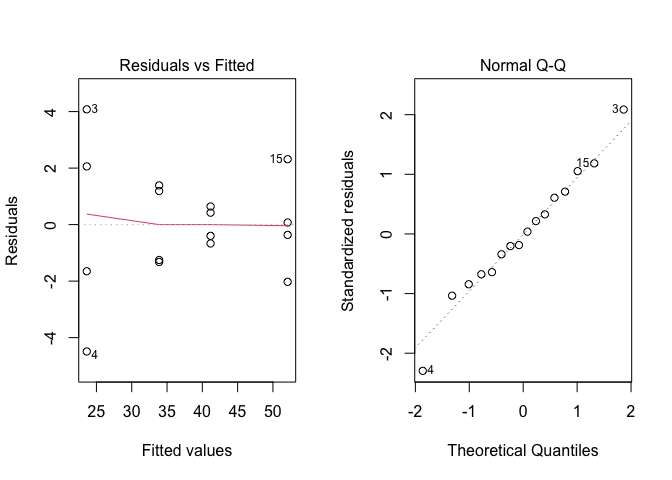
\includegraphics[width=0.9\linewidth]{_main_files/figure-latex/figName141-1} 

}

\caption{Analisi grafica dei residui per una prova di concimazione azotata del frumento}\label{fig:figName141}
\end{figure}

Da questo momento in avanti, diversamente a quanto abbiamo visto nei capitoli precedenti, l'analisi non prosegue con un test di confronto multiplo, che in questa situazione, se non del tutto errato, sarebbe comunque da considerare `improprio'. Infatti, quale senso avrebbe confrontare la risposta produttiva a 60 kg N ha\textsuperscript{-1} con quella a 120 kg N ha \textsuperscript{-1}? In realtà noi non siamo specificatamente interessati a queste due dosi, ma a qualunque altra dose nell'intervallo da 0 a 180 kg N ha\textsuperscript{-1}. Abbiamo selezionato quattro dosi per organizzare l'esperimento, ma resta il fatto che siamo interessati a definire una funzione di risposta per tutto l'intervallo delle dosi, non a confrontare le risposte a due dosi in particolare.

Per questo motivo, quando la variabile indipendente è una dose, l'analisi dei dati dovrebbe essere basata sull'impiego di un modello di regressione, in quanto ciò è più coerente con le finalità dell'esperimento, rispetto all'adozione di una procedura di confronto multiplo.

\hypertarget{definizione-del-modello-lineare-1}{%
\section{Definizione del modello lineare}\label{definizione-del-modello-lineare-1}}

Immaginiamo che, almeno nell'intervallo di dosi incluso nell'esperimento, l'effetto della concimazione azotata sulla produzione sia lineare. In effetti, l'andamento dei dati conferma questa impressione e, pertanto, poniamo il modello lineare nei termini usuali:

\[Y_i = b_0 + b_1 X_i + \varepsilon_i\]

dove \(Y\) è la produzione della parcella \(i\), trattata con la dose \(X_i\), \(b_0\) è l'intercetta (produzione a dose di azoto pari a 0) e \(b_1\) è la pendenza, cioè l'incremento di produzione per ogni incremento unitario della dose. La componente stocastica \(\varepsilon\) viene assunta omoscedastica e normalmente distribuita, con media 0 e deviazione standard \(\sigma\).

\hypertarget{stima-dei-parametri-3}{%
\section{Stima dei parametri}\label{stima-dei-parametri-3}}

Dobbiamo a questo punto individuare i parametri \(b_0\) e \(b_1\) in modo tale che la retta ottenuta sia la più vicina ai dati, cioè in modo da minimizzare gli scostamenti tra i valori di produzione osservati e quelli stimati dal modello (soluzione dei minimi quadrati). La funzione dei minimi quadrati è:

\[\begin{array}{l}
Q = \sum\limits_{i = }^N {\left( {{Y_i} - \hat Y} \right)^2 = \sum\limits_{i = }^N {{{\left( {{Y_i} - {b_0} - {b_1}{X_i}} \right)}^2}}  = } \\
 = \sum\limits_{i = }^N {\left( {Y_i^2 + b_0^2 + b_1^2X_i^2 - 2{Y_i}{b_0} - 2{Y_i}{b_1}{X_i} + 2{b_0}{b_1}{X_i}} \right)}  = \\
 = \sum\limits_{i = }^N {Y_i^2 + Nb_0^2 + b_1^2\sum\limits_{i = }^N {X_i^2 - 2{b_0}\sum\limits_{i = }^N {Y_i^2 - 2{b_1}\sum\limits_{i = }^N {{X_i}{Y_i} + } } } } 2{b_0}{b_1}\sum\limits_{i = }^N {{X_i}} 
\end{array}\]

Calcolando le derivate parziali rispetto a \(b_0\) e \(b_1\) che, al momento, sono le nostre incognite, ed eguagliandole a 0 si ottengono le seguenti formule risolutive:

\[{b_1} = \frac{{\sum\limits_{i = 1}^N {\left[ {\left( {{X_i} - {\mu _X}} \right)\left( {{Y_i} - {\mu _Y}} \right)} \right]} }}{{\sum\limits_{i = 1}^N {{{\left( {{X_i} - {\mu _X}} \right)}^2}} }}\]

e

\[{b_0} = {\mu _Y} - {b_1}{\mu _X}\]

Invece che svolgere i calcoli a mano, possiamo eseguire il fitting ai minimi quadrati con R. Possiamo notare che l'unica differenza tra questo modello di regressione e il modello ANOVA utilizzato poco sopra è che qui utilizziamo la variabile `Dose' come tale, senza trasformarla in un `factor'.

\begin{Shaded}
\begin{Highlighting}[]
\NormalTok{modelReg <-}\StringTok{ }\KeywordTok{lm}\NormalTok{(Yield }\OperatorTok{~}\StringTok{ }\NormalTok{Dose, }\DataTypeTok{data =}\NormalTok{ dataset)}
\KeywordTok{summary}\NormalTok{(modelReg)}
\CommentTok{## }
\CommentTok{## Call:}
\CommentTok{## lm(formula = Yield ~ Dose, data = dataset)}
\CommentTok{## }
\CommentTok{## Residuals:}
\CommentTok{##     Min      1Q  Median      3Q     Max }
\CommentTok{## -4.6537 -1.5350 -0.4637  1.9250  3.9163 }
\CommentTok{## }
\CommentTok{## Coefficients:}
\CommentTok{##              Estimate Std. Error t value Pr(>|t|)    }
\CommentTok{## (Intercept) 23.793750   0.937906   25.37 4.19e-13 ***}
\CommentTok{## Dose         0.154417   0.008356   18.48 3.13e-11 ***}
\CommentTok{## ---}
\CommentTok{## Signif. codes:  0 '***' 0.001 '**' 0.01 '*' 0.05 '.' 0.1 ' ' 1}
\CommentTok{## }
\CommentTok{## Residual standard error: 2.242 on 14 degrees of freedom}
\CommentTok{## Multiple R-squared:  0.9606, Adjusted R-squared:  0.9578 }
\CommentTok{## F-statistic: 341.5 on 1 and 14 DF,  p-value: 3.129e-11}
\end{Highlighting}
\end{Shaded}

Ora sappiamo che la relazione tra la dose di azoto e la risposta produttiva del frumento è:

\[ Y_i = 23.111 + 0.170 \times X_i \]

L'elemento stocastico \(\varepsilon_i\) è normalmente distribuito, con media 0 e deviazione standard 2.029 (vedi la voce `Residual standard error' nell'output sovrstante).

Come al solito, prima di qualunque altra considerazione, dobbiamo verificare la bontà del modello e il rispetto delle assunzioni di base, con una procedura che, per un modello di regressione, deve riguardare un maggior numero di aspetti rispetto ad un modello ANOVA.

\hypertarget{valutazione-della-bonta-del-modello}{%
\section{Valutazione della bontà del modello}\label{valutazione-della-bonta-del-modello}}

In primo luogo, è necessario verificare il rispetto delle assunzioni di base di normalità e omoscedasticità dei residui. Per questo, possiamo utilizzare gli stessi metodi impiegati per i modelli ANOVA, vale a dire un grafico dei residui verso gli attesi ed un QQ-plot dei residui standardizzati. In realtà, abbiamo già eseguito questo controllo con il modello ANOVA corrispondente e non vi è la necessità di ripeterlo con questo modello.

Dobbiamo invece assicurarci che i dati osservati siano ben descritti dal modello adottato, senza nessuna componente sistematica di mancanza d'adattamento. In altre parole, le osservazioni non debbono contraddire l'ipotesi che la risposta è lineare, salvo per le eventuali deviazioni casuali insite in qualunque esperimento. Per la verificà della \textbf{bontà di adattamento} possiamo utilizzare diverse procedure, che illustreremo di seguito.

\hypertarget{valutazione-grafica}{%
\subsection{Valutazione grafica}\label{valutazione-grafica}}

Nel modo più semplice, la bontà di adattamento può essere valutata attraverso un grafico dei valori attesi e dei valori osservati, come quello in Figura \ref{fig:figName142}. Notiamo che non c'è alcun elemento che faccia pensare ad una sistematica deviazione rispetto alle previsioni fatte dal modello.

\begin{figure}

{\centering 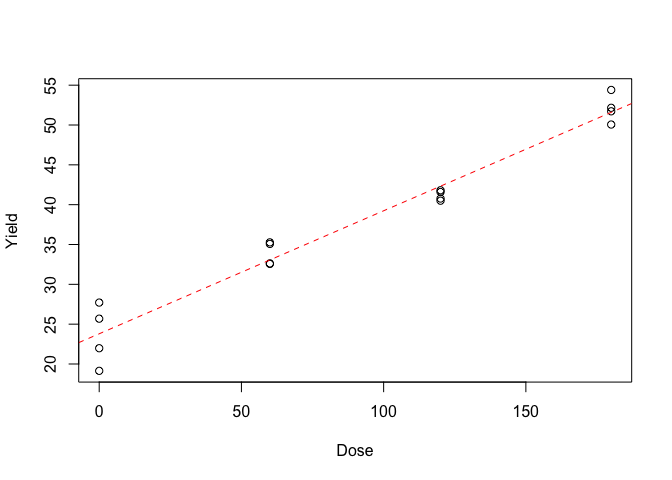
\includegraphics[width=0.9\linewidth]{_main_files/figure-latex/figName142-1} 

}

\caption{Risposta produttiva del frumento alla concimazione azotata: dati osservati (simboli) e valori attesi (linea tratteggiata).}\label{fig:figName142}
\end{figure}

\hypertarget{errori-standard-dei-parametri}{%
\subsection{Errori standard dei parametri}\label{errori-standard-dei-parametri}}

In secondo luogo, possiamo valutare gli errori standard delle stime dei parametri, che non debbono mai essere superiori alla metà del valore del parametro stimato, cosa che in questo caso è pienamente verificata. Se così non fosse, l'intervallo di confidenza del parametro, usualmente stimato utilizzando il doppio dell'errore standard, conterrebbe lo zero, il che equivarebbe a dire che, ad esempio, la pendenza `vera' (cioè quella della popolazione da cui il nostro campione è estratto) potrebbe essere nulla. In altre parole, la retta potrebbe essere `piatta', dimostrando l'inesistenza di relazione tra la dose di concimazione e la produzione della coltura. In realtà, nell'esempio in studio questo dubbio non sussiste.

\hypertarget{test-f-per-la-mancanza-dadattamento}{%
\subsection{Test F per la mancanza d'adattamento}\label{test-f-per-la-mancanza-dadattamento}}

In terzo luogo, possiamo analizzare i residui della regressione, cioè gli scostamenti dei punti rispetto alla retta e, in particolare, la somma dei loro quadrati. Possiamo vedere che questo valore è pari a 70.37, ed è più alto di quello del corrispondente modello ANOVA, impiegato in precedenza (61.22):

\begin{Shaded}
\begin{Highlighting}[]
\KeywordTok{anova}\NormalTok{(modelReg)}
\CommentTok{## Analysis of Variance Table}
\CommentTok{## }
\CommentTok{## Response: Yield}
\CommentTok{##           Df  Sum Sq Mean Sq F value    Pr(>F)    }
\CommentTok{## Dose       1 1716.80 1716.80  341.54 3.129e-11 ***}
\CommentTok{## Residuals 14   70.37    5.03                      }
\CommentTok{## ---}
\CommentTok{## Signif. codes:  0 '***' 0.001 '**' 0.01 '*' 0.05 '.' 0.1 ' ' 1}
\end{Highlighting}
\end{Shaded}

Il risultato è perfettamente normale, dato che il residuo del modello ANOVA contiene solo la misura dello scostamento di ogni dato rispetto alla media del suo gruppo, che si può considerare `errore puro', mentre il residuo della regressione, oltre all'errore puro, contiene anche una componente detta `mancanza d'adattamento' (lack of fit), misurabile con lo scostamento di ogni media dalla linea di regressione. In effetti, la regressione lineare è solo un'approssimazione della reale relazione biologica tra la concimazione e la produzione del frumento.

Insomma, il modello di regressione è un modello che ha sempre minor capacità descrittiva rispetto ad un modello ANOVA. La differenza può essere quantificata utilizzando le devianze dei rispettivi residui:

\[\textrm{Lack of fit} = 70.37 - 61.22 = 9.15\]

Bisogna però anche dire che il modello di regressione è più parsimonioso, nel senso che ci ha costretto a stimare solo due parametri (\(b_0\) e \(b_1\)), mentre il modello ANOVA ce ne ha fatti stimare quattro (\(\mu\), \(\alpha_2\), \(\alpha_3\) e \(\alpha_4\), considerando che \(\alpha_1 = 0\)). Quindi il residuo del modello di regressione ha 14 gradi di libertà (16 dati meno due parametri stimati), mentre il residuo del modello ANOVA ne ha 12 (16 - 4). La componente di lack of fit ha quindi 14 - 12 = 2 gradi di libertà. Ci chiediamo, questa componente di lack of fit è significativamente più grande dell'errore puro?

L'ipotesi nulla di assenza di lack of fit può essere testata con un test di F, per il confronto di due varianze: se questo è significativo allora la componente di mancanza d'adattamento non è trascurabile, ed il modello di regressione dovrebbe essere rifiutato. L'espressione è:

\[ F_{lack} = \frac{\frac{RSS_r - RSS_a}{DF_r-DF_a} } {\frac{RSS_a}{DF_a}} = \frac{MS_{lack}}{MSE_a}\]

dove RSS\textsubscript{r} è la devianza residua della regressione con i sui gradi di liberta DF\textsubscript{r} e RSS\textsubscript{a} è la devianza residua del modello ANOVA, con i suoi gradi di libertà DF\textsubscript{a}. In R, il test F per la mancanza d'adattamento può essere eseguito con la funzione `anova()', confrontando i due modelli alternativi:

\begin{Shaded}
\begin{Highlighting}[]
\KeywordTok{anova}\NormalTok{(modelReg, model)}
\CommentTok{## Analysis of Variance Table}
\CommentTok{## }
\CommentTok{## Model 1: Yield ~ Dose}
\CommentTok{## Model 2: Yield ~ factor(Dose)}
\CommentTok{##   Res.Df    RSS Df Sum of Sq      F Pr(>F)}
\CommentTok{## 1     14 70.373                           }
\CommentTok{## 2     12 61.219  2    9.1542 0.8972 0.4334}
\end{Highlighting}
\end{Shaded}

Vediamo che non otteniamo risultati significativi (P = 0.4334). Ciò supporta l'idea che non vi sia mancanza d'adattamento e quindi la regressione fornisca una descrizione altrettanto adeguata dei dati sperimentali rispetto al più `complesso' modello ANOVA. Scegliamo quindi il modello di regressione, in quanto più semplice, nel rispetto del principio del rasoio di Occam.

\hypertarget{test-f-per-la-bonta-di-adattamento-e-coefficiente-di-determinazione}{%
\subsection{Test F per la bontà di adattamento e coefficiente di determinazione}\label{test-f-per-la-bonta-di-adattamento-e-coefficiente-di-determinazione}}

Abbiamo dimostrato che il modello di regressione non è significativamente peggiore del modello ANOVA corrispondente. Un approccio alternativo per dimostrare la bontà di adattamento è verificare se il modello di regressione è significativamente migliore di un modello `nullo'. Ricordiamo che con il modello `nullo' (\(Y_i = \mu + \varepsilon_i\)) si assume che la risposta sia costante e pari alla media di tutti i dati, escludendo così ogni effetto della dose di concimazione. La devianza del residuo di un modello nullo non è altro che la devianza totale dei dati, che risulta pari a 1787.178:

\begin{Shaded}
\begin{Highlighting}[]
\NormalTok{modNull <-}\StringTok{ }\KeywordTok{lm}\NormalTok{(Yield }\OperatorTok{~}\StringTok{ }\DecValTok{1}\NormalTok{, }\DataTypeTok{data =}\NormalTok{ dataset)}
\KeywordTok{deviance}\NormalTok{(modNull)}
\CommentTok{## [1] 1787.178}
\end{Highlighting}
\end{Shaded}

Abbiamo visto che la devianza del modello di regressione è pari a 70.37: la differenza (1716.81) rappresenta la `bontà di adattamento', cioè una misura di quanto migliora il potere descrittivo del modello aggiungendo l'effetto `dose'. Quindi, un test di F per la bontà di adattamento può essere costruito come:

\[ F_{good} = \frac{\frac{RSS_t - RSS_r}{DF_t - DF_r} } {\frac{RSS_r}{DF_r}} = \frac{MS_{good}}{MSE_r}\]

dove RSS\textsubscript{t} è la devianza totale dei dati con i sui gradi di liberta DF\textsubscript{t}. In R, il test F per la bontà d'adattamento può essere eseguito con la funzione `anova()', senza la necessità di includere come argomento il modello `nullo':

\begin{Shaded}
\begin{Highlighting}[]
\KeywordTok{anova}\NormalTok{(modelReg)}
\CommentTok{## Analysis of Variance Table}
\CommentTok{## }
\CommentTok{## Response: Yield}
\CommentTok{##           Df  Sum Sq Mean Sq F value    Pr(>F)    }
\CommentTok{## Dose       1 1716.80 1716.80  341.54 3.129e-11 ***}
\CommentTok{## Residuals 14   70.37    5.03                      }
\CommentTok{## ---}
\CommentTok{## Signif. codes:  0 '***' 0.001 '**' 0.01 '*' 0.05 '.' 0.1 ' ' 1}
\end{Highlighting}
\end{Shaded}

Vediamo che in questo caso l'ipotesi nulla deve essere rifiutata: la varianza spiegata dalla regressione è significativamente maggiore di quella del residuo.

Più frequentemente, la devianza spiegata dalla regressione viene rapportata alla devianza totale, per individuare quanta parte della variabilità dei dati è spiegata dal modello prescelto. Questa proporzione definisce il cosidetto \textbf{coefficente di determinazione} o R\textsuperscript{2}:

\[R^2 = \frac{SS_{reg}}{SS_{tot}} = \frac{1716.81}{1787.18} = 0.961\]

Questa statistica varia da 0 ad 1 e la regressione è tanto migliore quanto più essa si avvicina ad 1. In realtà il coefficiente di determinazione è visibile nell'output della funzione `summary()' applicata all'oggetto `modelReg' (vedi più sopra).

\hypertarget{previsioni}{%
\section{Previsioni}\label{previsioni}}

Dato che il modello ha mostrato di funzionare bene, con prudenza possiamo utilizzarlo per prevedere le produzioni a dosi intermedie, che non sono state incluse in prova. Ovviamente ci si deve mantenere entro il valore massimo e quello minimo inclusi in prova. In R, ciò è possibile utilizzando la funzione `predict()', passando come argomento le dosi alle quali effettuare la previsione, organizzate in un data frame. Ad esempio, se si vuole prevedere la produzione a 30 e 80 kg N ha\textsuperscript{-1}, il codice è:

\begin{Shaded}
\begin{Highlighting}[]
\NormalTok{pred <-}\StringTok{ }\KeywordTok{predict}\NormalTok{(modelReg, }\DataTypeTok{newdata=}\KeywordTok{data.frame}\NormalTok{(}\DataTypeTok{Dose=}\KeywordTok{c}\NormalTok{(}\DecValTok{30}\NormalTok{, }\DecValTok{80}\NormalTok{)), }\DataTypeTok{se=}\NormalTok{T)}
\NormalTok{pred}
\CommentTok{## $fit}
\CommentTok{##        1        2 }
\CommentTok{## 28.42625 36.14708 }
\CommentTok{## }
\CommentTok{## $se.fit}
\CommentTok{##         1         2 }
\CommentTok{## 0.7519981 0.5666999 }
\CommentTok{## }
\CommentTok{## $df}
\CommentTok{## [1] 14}
\CommentTok{## }
\CommentTok{## $residual.scale}
\CommentTok{## [1] 2.242025}
\end{Highlighting}
\end{Shaded}

E'anche possibile effettuare la previsione inversa, cioè chiedere ai dati qual è la dose a cui corrisponde una produzione di 45 q/ha. In questo caso dobbiamo tener presente che l'equazione inversa è:

\[X = \frac{Y - b_0}{b_1}\]

Per calcolare il risultato possiamo utilizzare la funzione `deltaMethod()', nel package `car', che ci calcola anche gli errori standard con il metodo della propagazione degli errori:

\begin{Shaded}
\begin{Highlighting}[]
\NormalTok{car}\OperatorTok{::}\KeywordTok{deltaMethod}\NormalTok{(modelReg, }\StringTok{"(45 - b0)/b1"}\NormalTok{, }
                 \DataTypeTok{parameterNames=}\KeywordTok{c}\NormalTok{(}\StringTok{"b0"}\NormalTok{, }\StringTok{"b1"}\NormalTok{))}
\CommentTok{##              Estimate       SE    2.5 % 97.5 %}
\CommentTok{## (45 - b0)/b1 137.3314   4.4424 128.6244 146.04}
\end{Highlighting}
\end{Shaded}

Il procedimento sopra descritto è molto comune, per esempio nei laboratori chimici, dove viene utilizzato nella fase di calibrazione di uno strumento. Una volta che la retta di calibrazione è stata individuate, essa viene utilizzata per determinare le concentrazioni incognite di campioni per i quali sia stata misurata la risposta.

\begin{center}\rule{0.5\linewidth}{\linethickness}\end{center}

\hypertarget{per-approfondire-un-po-8}{%
\section{Per approfondire un po'\ldots{}}\label{per-approfondire-un-po-8}}

\begin{enumerate}
\def\labelenumi{\arabic{enumi}.}
\tightlist
\item
  Draper, N.R., Smith, H., 1981. Applied Regression Analysis, in: Applied Regression. John Wiley \& Sons, Inc., IDA, pp.~224--241.
\item
  Faraway, J.J., 2002. Practical regression and Anova using R. \url{http://cran.r-project.org/doc/contrib/Faraway-PRA.pdf}, R.
\end{enumerate}

\hypertarget{la-regressione-non-lineare}{%
\chapter{La regressione non-lineare}\label{la-regressione-non-lineare}}

I fenomeni biologici, come ad esempio la crescita di una coltura, la cinetica degradativa degli erbicidi nel terreno, la risposta produttiva delle colture a densità crescenti di malerbe o a dosi crescenti di concime, la risposta fitotossica di una specie infestante alla dose di un erbicida, hanno in genere andamenti curvilinei, posseggono punti di massimo o minimo, flessi e, soprattutto, hanno frequentemente asintoti. Pertanto, difficilmente possono essere descritti con funzioni lineari, a meno che non ci accontentiamo di approssimare localmente l'andamento dei dati, in un intervallo ristretto della variabile indipendente.

Da un punto di vista pratico, è quindi fondamentale saper adattare ai dati funzioni curvilinee di ogni tipo. Introduciamo il problema con un esempio.

\hypertarget{caso-studio-degradazione-di-un-erbicida-nel-terreno}{%
\section{Caso studio: degradazione di un erbicida nel terreno}\label{caso-studio-degradazione-di-un-erbicida-nel-terreno}}

Un suolo è stato trattato con metamitron (un erbicida) alla concentrazione di 100 ng g\textsuperscript{1}. Dopo essere stato opportunamente mescolato, è stato distribuito in 24 contenitori di alluminio e posto in cella climatica alla temperatura di 20 °C. In 8 tempi diversi dopo l'inizio del saggio, sono stati prelevati 3 contenitori e sottoposti ad analisi chimica per la determinazione della concentrazione residua dell'erbicida. I dati osservati sono disponibili nel package `aomisc', che deve quindi essere installato e caricato in memoria, secondo le istruzioni fornite nell'introduzione.

\begin{Shaded}
\begin{Highlighting}[]
\KeywordTok{library}\NormalTok{(aomisc)}
\KeywordTok{data}\NormalTok{(degradation)}
\KeywordTok{head}\NormalTok{(degradation, }\DecValTok{10}\NormalTok{)}
\CommentTok{##    Time   Conc}
\CommentTok{## 1     0  96.40}
\CommentTok{## 2    10  46.30}
\CommentTok{## 3    20  21.20}
\CommentTok{## 4    30  17.89}
\CommentTok{## 5    40  10.10}
\CommentTok{## 6    50   6.90}
\CommentTok{## 7    60   3.50}
\CommentTok{## 8    70   1.90}
\CommentTok{## 9     0 102.30}
\CommentTok{## 10   10  49.20}
\end{Highlighting}
\end{Shaded}

Per prima cosa, plottiamo i dati osservati (Figura \ref{fig:figName151}); vediamo che l'andamento della concentrazione nel tempo è chiaramente curvilineo e, di conseguenza, non possiamo utilizzare la regressione lineare semplice, esposta nel capitolo precedente.

\begin{figure}

{\centering 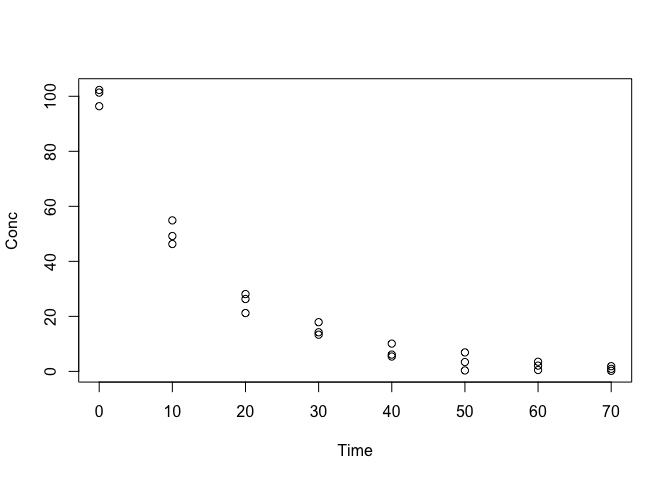
\includegraphics[width=0.9\linewidth]{_main_files/figure-latex/figName151-1} 

}

\caption{Degradazione di metamitron nel terreno}\label{fig:figName151}
\end{figure}

In realtà, possiamo ancora utilizzare la stessa equazione generale che abbiamo introdotto nel capitolo 4, cioè:

\[ Y_i = f(X_i, \theta) + \varepsilon_i \]

In questa funzione, \(X\) è il tempo, \(Y\) la concentrazione, \(\theta\) sono i parametri del modello (da stimare) ed \(\varepsilon\) sono i residui, che si assumono omoscedastici e normalmente distribuiti. La differenza sta nel fatto che \(f\) è non lineare.

\hypertarget{scelta-della-funzione}{%
\section{Scelta della funzione}\label{scelta-della-funzione}}

Uno dei criteri fondamentali, seppur empirico, per la selezione di una funzione non-lineare è quello di considerarne la forma, in relazione al fenomeno biologico in studio. Per questo scopo, le equazioni sno spesso classificate in base alla forma, come:

\begin{enumerate}
\def\labelenumi{\arabic{enumi}.}
\tightlist
\item
  Lineari (es. retta)
\item
  Convesse/concave (es. funzione esponenziale, funzione di potenza, funzione logaritmica, iperbole)
\item
  Sigmoidali (es. funzione logistica, funzione di Gompertz)
\item
  Curve con massimi/minimi (esequazione di Brain-Cousens, equazione di Braggs)
\end{enumerate}

La descrizione di queste equazioni esula dallo scopo di questo libro, anche se il loro studio può essere di notevole interesse, anche per un biologo o un agronomo. Infatti, riuscire a tradurre nel linguaggio matematico un fenomeno biologico è forse uno degli obiettivi più affascinanti che un ricercatore si possa porre. Per chi fosse interessato, riportiamo in calce al capitolo alcuni interessanti riferimenti.

Noi ci poniamo nella situazione più comune, quella in cui la scelta del modello viene fatta in base all'esperienza o alle informazioni disponibili in letteratura. In questo caso, le conoscenze relative alla cinetica di degradazione dei composti chimici ci suggeriscono un'equazione di decadimento esponenziale (cinetica del primo ordine), così definita:

\[Y_i = A e^{-k \,X_i} + \varepsilon_i\]

dove A è la concentrazione iniziale e \(k\) e il tasso di degradazione (costante nel tempo). Come anticipato, la componente stocastica \(\varepsilon\) si assume normalmente distribuita e omoscedastica.

\hypertarget{stima-dei-parametri-4}{%
\section{Stima dei parametri}\label{stima-dei-parametri-4}}

Dopo aver definito \(f\), dobbiamo stimare i parametri \(A\) e \(k\). In generale esistono tre tecniche fondamentali:

\begin{enumerate}
\def\labelenumi{\arabic{enumi}.}
\tightlist
\item
  linearizzazione della funzione tramite trasformazione delle variabili;
\item
  approssimazione della vera funzione curvilinea con una polinomiale in X;
\item
  adattamento ai dati sperimentali di funzioni curvilinee, tramite metodiche di regressione non-lineare.
\end{enumerate}

\hypertarget{linearizzazione-della-funzione}{%
\subsection{Linearizzazione della funzione}\label{linearizzazione-della-funzione}}

Nel caso specifico, prendendo il logaritmo di entrambe le parti dell'equazione esponenziale, otteniamo la seguente equazione:

\[ log(Y) = log(A) - k \, X \]

Quindi, se trasformiamo la Y (Concentrazione) nel suo logaritmo, possiamo utilizzare un modello di regressione lineare semplice per la stima dei parametri. Ovviamente, otterremo, come intercetta, il logaritmo della concentrazione iniziale e, come pendenza, otterremo un valore negativo per \(k\), in quanto la retta è decrescente.

\begin{Shaded}
\begin{Highlighting}[]
\NormalTok{mod <-}\StringTok{ }\KeywordTok{lm}\NormalTok{(}\KeywordTok{log}\NormalTok{(Conc) }\OperatorTok{~}\StringTok{ }\NormalTok{Time, }\DataTypeTok{data=}\NormalTok{degradation)}
\KeywordTok{summary}\NormalTok{(mod)}
\CommentTok{## }
\CommentTok{## Call:}
\CommentTok{## lm(formula = log(Conc) ~ Time, data = degradation)}
\CommentTok{## }
\CommentTok{## Residuals:}
\CommentTok{##      Min       1Q   Median       3Q      Max }
\CommentTok{## -2.11738 -0.09583  0.05336  0.31166  1.01243 }
\CommentTok{## }
\CommentTok{## Coefficients:}
\CommentTok{##              Estimate Std. Error t value Pr(>|t|)    }
\CommentTok{## (Intercept)  4.662874   0.257325   18.12 1.04e-14 ***}
\CommentTok{## Time        -0.071906   0.006151  -11.69 6.56e-11 ***}
\CommentTok{## ---}
\CommentTok{## Signif. codes:  0 '***' 0.001 '**' 0.01 '*' 0.05 '.' 0.1 ' ' 1}
\CommentTok{## }
\CommentTok{## Residual standard error: 0.6905 on 22 degrees of freedom}
\CommentTok{## Multiple R-squared:  0.8613, Adjusted R-squared:  0.855 }
\CommentTok{## F-statistic: 136.6 on 1 and 22 DF,  p-value: 6.564e-11}
\end{Highlighting}
\end{Shaded}

Le funzioni non-lineari che possono essere trasformate in lineari sono dette \emph{linearizzabili} e hanno il vantaggio di semplificare molto i calcoli richiesti per la stima dei parametri. Un grave svantaggio è dato dal fatto che, trasformando la Y, si trasforma anche la distribuzione degli errori e quindi bisogna verificare che le assunzioni di base dei modelli lineari (omogeneità delle varianze e normalità dei residui) siano valide nella scala trasformata.

\begin{Shaded}
\begin{Highlighting}[]
\KeywordTok{par}\NormalTok{(}\DataTypeTok{mfrow =} \KeywordTok{c}\NormalTok{(}\DecValTok{1}\NormalTok{,}\DecValTok{2}\NormalTok{))}
\KeywordTok{plot}\NormalTok{(mod, }\DataTypeTok{which =} \DecValTok{1}\NormalTok{)}
\KeywordTok{plot}\NormalTok{(mod, }\DataTypeTok{which =} \DecValTok{2}\NormalTok{)}
\end{Highlighting}
\end{Shaded}

\begin{figure}

{\centering 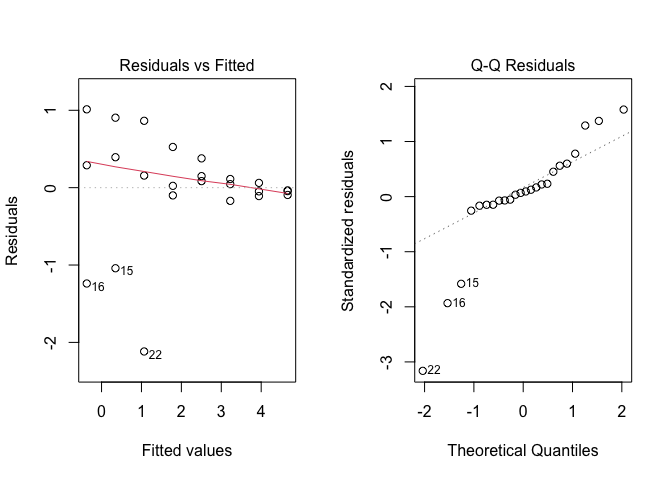
\includegraphics[width=0.9\linewidth]{_main_files/figure-latex/figName152-1} 

}

\caption{Linearizzazione di una funzione esponenziale.}\label{fig:figName152}
\end{figure}

Il grafico dei residui (Figura \ref{fig:figName152} ) suggerisce che questi sono inversamente proporzionali ai valori attesi (più alto il logaritmo della concentrazione più bassi i residui). Questo fa sospettare che le varianze potrebbero essere omogenee sulla scala originale, impedendoci quindi di analizzare i dati nella scala trasformata.

Per completezza, dobbiamo comunque dire che, qualora le assunzioni di base fossero rispettate nella scala trasformata, il metodo della linearizzazione rappresenterebbe una tecnica corretta ed affidabile per l'analisi dei dati.

\hypertarget{approssimazione-della-vera-funzione-tramite-una-polinomiale-in-x}{%
\subsection{Approssimazione della vera funzione tramite una polinomiale in X}\label{approssimazione-della-vera-funzione-tramite-una-polinomiale-in-x}}

Molte andamenti non-lineari possono essere approssimati tramite funzioni polinomiali di ordine \textit{n}. Le funzioni polinomiali sono molto flessibili; contengono la funzione lineare come caso particolare (n = 1) e permettono di descrivere curvature anche molto complesse, semplicemente aumentando l' ordine della funzione. In questo modo, è possibile ottenere un adattamento ai dati sperimentali teoricamente anche perfetto.

Le funzioni polinomiali sono un tipico esempio di funzioni curvilinee, ma lineari nei parametri; esse possono essere trattate ricorrendo alle metodiche di calcolo normalmente utilizzate per la regressione lineare.

Gli svantaggi delle funzioni polinomiali sono relativi al fatto che queste presentano raramente giustificazione biologica. Per esempio, con le funzioni polinomiali non è possibile descrivere relazioni asintotiche, che sono invece molto comuni in biologia. Nel nostro esempio si potrebbe utilizzare una funzione polinomiale di II grado (parabola), che, con il suo braccio decrescente, potrebbe descrivere la degradazione di un erbicida in modo sufficientemente buono.

Eseguiamo il fitting con R, utilizzando l'usuale funzione `lm()'. Successivamente, utilizziamo la funzione `predict()' per generare valori attesi per una sequenza temporale da 0 a 70 giorni e plottarli.

\begin{Shaded}
\begin{Highlighting}[]
\NormalTok{mod2 <-}\StringTok{ }\KeywordTok{lm}\NormalTok{(Conc }\OperatorTok{~}\StringTok{ }\NormalTok{Time }\OperatorTok{+}\StringTok{ }\KeywordTok{I}\NormalTok{(Time}\OperatorTok{^}\DecValTok{2}\NormalTok{), }\DataTypeTok{data=}\NormalTok{degradation)}
\NormalTok{pred <-}\StringTok{ }\KeywordTok{predict}\NormalTok{(mod2, }\DataTypeTok{newdata =} \KeywordTok{data.frame}\NormalTok{(}\DataTypeTok{Time =} \KeywordTok{seq}\NormalTok{(}\DecValTok{0}\NormalTok{, }\DecValTok{70}\NormalTok{, }\DataTypeTok{by =} \FloatTok{0.1}\NormalTok{)))}
\KeywordTok{plot}\NormalTok{(Conc }\OperatorTok{~}\StringTok{ }\NormalTok{Time, }\DataTypeTok{data=}\NormalTok{degradation)}
\KeywordTok{lines}\NormalTok{(pred }\OperatorTok{~}\StringTok{ }\KeywordTok{seq}\NormalTok{(}\DecValTok{0}\NormalTok{, }\DecValTok{70}\NormalTok{, }\DataTypeTok{by =} \FloatTok{0.1}\NormalTok{), }\DataTypeTok{col =} \StringTok{"red"}\NormalTok{)}
\end{Highlighting}
\end{Shaded}

\begin{figure}

{\centering 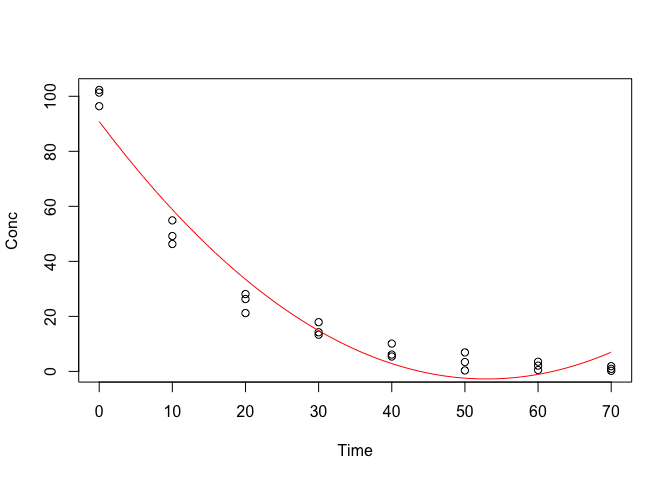
\includegraphics[width=0.9\linewidth]{_main_files/figure-latex/figName153-1} 

}

\caption{Approssimazione della cinetica di degradazione con una funzione polinomiale (parabola)}\label{fig:figName153}
\end{figure}

Vediamo come la funzione inserita, mentre approssima abbastanza bene i dati nell'intervallo da 0 a 40 giorni, successivamente mostra una ricrescita, che non ha alcun senso biologico (Figura \ref{fig:figName153} ).

In generale, le polinomiali sono utilizzate quando non si hanno conoscenze `a priori' sul fenomeno in studio e sia necessario approssimarlo con una funzione curvilinea, in un intervallo della X molto ristretto, senza la necessità di estrapolare previsioni al di fuori di questo intervallo. Per questi motivi, il campo d'impiego delle funzioni polinomiale è abbastanza ristretto.

\hypertarget{minimi-quadrati-non-lineari}{%
\subsection{Minimi quadrati non-lineari}\label{minimi-quadrati-non-lineari}}

La terza strada, quella più percorsa, è utilizzare metodiche di regressione non-lineare, basate su algoritmi numerici di ricerca delle stime dei minimi quadrati, come il metodo di Gauss-Newton. Nel principio, questo metodo funziona partendo da stime iniziali approssimate dei parametri, che vengono corrette in ogni iterazione successiva fino ad ottenere la convergenza sui valori che minimizzano lo scostamento tra i valori osservati e quelli previsti dalla funzione. Ovviamente, trattandosi di metodi iterativi, le stime ottenute sono solo un'approssimazione dei valori reali, ma più che accettabile per le nostre finalità.

\hypertarget{la-regressione-non-lineare-con-r}{%
\section{La regressione non-lineare con R}\label{la-regressione-non-lineare-con-r}}

La funzione più comune in R per la parametrizzazione di funzioni non-lineari è `nls()'. Nella chiamata alla funzione dobbiamo anche fornire stime iniziali per i valori dei parametri. Ottenere queste stime è facile pensando al loro significato biologico: \(A\) è la concentrazione iniziale e quindi una stima ragionevole è data dal valor medio osservato al tempo 0 (100). Il parametro \(k\) è invece il tasso di degradazione relativo; possiamo notare che nei primi 10 giorni la concentrazione si riduce della metà circa, cioè si abbassa mediamente un po' più del 5\% al giorno. Possiamo quindi assegnare a \(k\) un valore iniziale pari a 0.05.

\begin{Shaded}
\begin{Highlighting}[]
\NormalTok{modNlin <-}\StringTok{ }\KeywordTok{nls}\NormalTok{(Conc }\OperatorTok{~}\StringTok{ }\NormalTok{A}\OperatorTok{*}\KeywordTok{exp}\NormalTok{(}\OperatorTok{-}\NormalTok{k}\OperatorTok{*}\NormalTok{Time), }
               \DataTypeTok{start=}\KeywordTok{list}\NormalTok{(}\DataTypeTok{A=}\DecValTok{100}\NormalTok{, }\DataTypeTok{k=}\FloatTok{0.05}\NormalTok{), }
               \DataTypeTok{data=}\NormalTok{degradation)}
\KeywordTok{summary}\NormalTok{(modNlin)}
\CommentTok{## }
\CommentTok{## Formula: Conc ~ A * exp(-k * Time)}
\CommentTok{## }
\CommentTok{## Parameters:}
\CommentTok{##    Estimate Std. Error t value Pr(>|t|)    }
\CommentTok{## A 99.634902   1.461047   68.19   <2e-16 ***}
\CommentTok{## k  0.067039   0.001887   35.53   <2e-16 ***}
\CommentTok{## ---}
\CommentTok{## Signif. codes:  0 '***' 0.001 '**' 0.01 '*' 0.05 '.' 0.1 ' ' 1}
\CommentTok{## }
\CommentTok{## Residual standard error: 2.621 on 22 degrees of freedom}
\CommentTok{## }
\CommentTok{## Number of iterations to convergence: 5 }
\CommentTok{## Achieved convergence tolerance: 4.33e-07}
\end{Highlighting}
\end{Shaded}

\hypertarget{verifica-della-bonta-del-modello}{%
\section{Verifica della bontà del modello}\label{verifica-della-bonta-del-modello}}

Le assunzioni parametriche di base relative ai modelli non-lineari sono le stesse dei modelli lineari e, di conseguenza, gli strumenti diagnostici sono analoghi. Bisogna tuttavia menzionare il fatto che, dato l'impiego di metodi iterativi per la ricerca dei valori dei parametri, tutti i risultati a cui si perviene (stima dei parametri, della varianza residua e numero dei gradi di libertà relativi) sono solo una approssimazione di quelli reali. Per questo motivo, nel caso non-lineare i metodi grafici (analisi dei residui) sono largamente preferiti.

\hypertarget{analisi-grafica-dei-residui-1}{%
\subsection{Analisi grafica dei residui}\label{analisi-grafica-dei-residui-1}}

L'analisi grafica dei residui viene eseguita in modo del tutto analogo a quanto visto per la regressione lineare. In primo luogo, verifichiamo le assunzioni di base di normalità e omoscedasticità, mediante il metodo `plot()' per l'oggetto `nls', che è disponibile nel package `aomisc', già caricato in precedenza.

\begin{Shaded}
\begin{Highlighting}[]
\KeywordTok{par}\NormalTok{(}\DataTypeTok{mfrow=}\KeywordTok{c}\NormalTok{(}\DecValTok{1}\NormalTok{,}\DecValTok{2}\NormalTok{))}
\KeywordTok{plot}\NormalTok{(modNlin, }\DataTypeTok{which =} \DecValTok{1}\NormalTok{)}
\KeywordTok{plot}\NormalTok{(modNlin, }\DataTypeTok{which =} \DecValTok{2}\NormalTok{)}
\end{Highlighting}
\end{Shaded}

\begin{figure}

{\centering 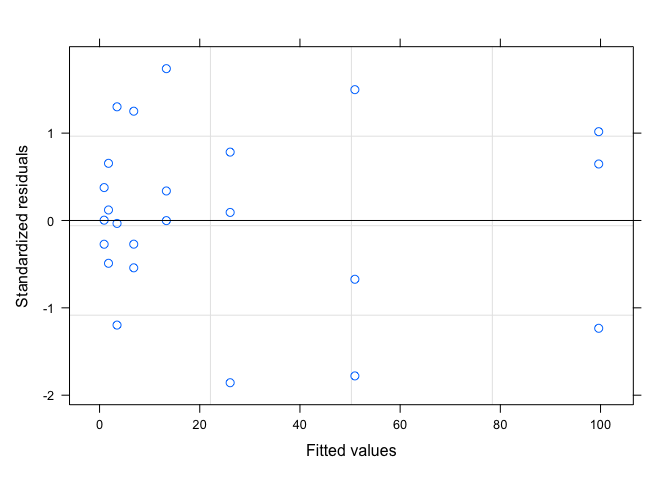
\includegraphics[width=0.9\linewidth]{_main_files/figure-latex/figName154-1} 

}

\caption{Analisi grafica dei residui per la regressione non-lineare, relativa alla degradazione di metamitron nel suolo}\label{fig:figName154}
\end{figure}

La Figura \ref{fig:figName154} non mostra deviazioni rispetto agli assunti di base. Pertanto, proseguiamo l'analisi grafica della bontà di adattamento, verificando il plot dei valori attesi e di quelli osservati (Figure \ref{fig:figName155}). Questo grafico, per gli oggetti `nls' può essere ottenuto velocemente utilizzando la funzione `plotnls()', nel package `aomisc'.

\begin{Shaded}
\begin{Highlighting}[]
\KeywordTok{library}\NormalTok{(lattice)}
\KeywordTok{plotnls}\NormalTok{(modNlin)}
\end{Highlighting}
\end{Shaded}

\begin{figure}

{\centering 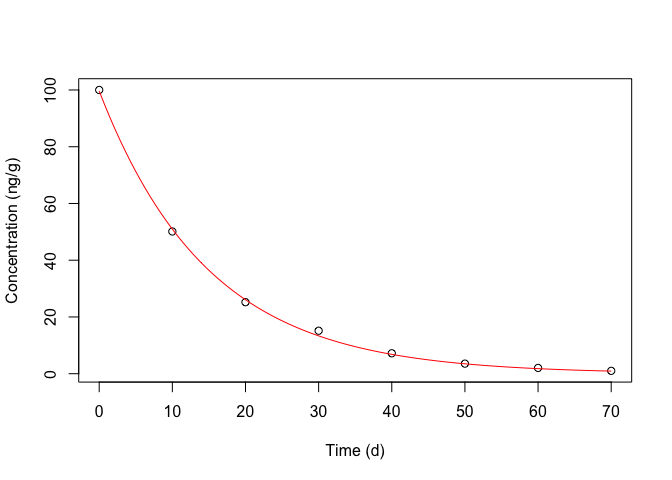
\includegraphics[width=0.9\linewidth]{_main_files/figure-latex/figName155-1} 

}

\caption{Cinetica di degradazione di metamitron nel suolo: i punti mostrano i valori osservati, la linea mostra i valori attesi con l'equazione esponziale.}\label{fig:figName155}
\end{figure}

\hypertarget{test-f-per-la-mancanza-di-adattamento-approssimato}{%
\subsection{Test F per la mancanza di adattamento (approssimato)}\label{test-f-per-la-mancanza-di-adattamento-approssimato}}

Se abbiamo le repliche (come nellesempio in studio) possiamo effettuare il fitting di un modello ANOVA. Come abbiamo detto nel capitolo precedente, nel modello ANOVA i valori attesi sono costituiti dalle medie dei trattamenti (tempi e livelli di densità, rispettivamente per i due esempi) e lo scostamento di ogni dato rispetto alla `sua' media è evidentemente dovuto solo all'errore sperimentale `puro'. Nel modello di regressione, invece, esiste una componente aggiuntiva di errore, cioè lo scostamento di ogni media dalla curva di regressione. Questa componente si chiama mancanza d'adattamento e può essere stimata per differenza.

\begin{Shaded}
\begin{Highlighting}[]
\NormalTok{modAov <-}\StringTok{ }\KeywordTok{lm}\NormalTok{(Conc }\OperatorTok{~}\StringTok{ }\KeywordTok{factor}\NormalTok{(Time), }\DataTypeTok{data=}\NormalTok{degradation)}
\KeywordTok{anova}\NormalTok{(modAov)}
\CommentTok{## Analysis of Variance Table}
\CommentTok{## }
\CommentTok{## Response: Conc}
\CommentTok{##              Df  Sum Sq Mean Sq F value    Pr(>F)    }
\CommentTok{## factor(Time)  7 24698.4  3528.3  415.29 < 2.2e-16 ***}
\CommentTok{## Residuals    16   135.9     8.5                      }
\CommentTok{## ---}
\CommentTok{## Signif. codes:  0 '***' 0.001 '**' 0.01 '*' 0.05 '.' 0.1 ' ' 1}
\NormalTok{SSa <-}\StringTok{ }\KeywordTok{anova}\NormalTok{(modAov)[}\DecValTok{2}\NormalTok{,}\DecValTok{2}\NormalTok{]}
\NormalTok{SSa}
\CommentTok{## [1] 135.9387}
\end{Highlighting}
\end{Shaded}

Inseriamo il tempo come fattore (quindi variabile qualitativa, non quantitativa) e notiamo che la devianza del residuo è pari a 135.9. La varianza del residuo del modello di regressione si ottiene facendo la somma dei quadrati degli scarti dei dati rispetto ai valori attesi.

\begin{Shaded}
\begin{Highlighting}[]
\NormalTok{SSr <-}\StringTok{ }\KeywordTok{sum}\NormalTok{(}\KeywordTok{residuals}\NormalTok{(modNlin)}\OperatorTok{^}\DecValTok{2}\NormalTok{)}
\NormalTok{SSr}
\CommentTok{## [1] 151.1766}
\end{Highlighting}
\end{Shaded}

Come ci aspettavamo, il modello di regressione ha una devianza più alta, in quanto questa contiene la componente di mancanza d'adattamento, pari alla differenza tra SSa e SSr, cioè:

\begin{Shaded}
\begin{Highlighting}[]
\NormalTok{SSl <-}\StringTok{ }\NormalTok{SSr }\OperatorTok{-}\StringTok{ }\NormalTok{SSa}
\NormalTok{SSl}
\CommentTok{## [1] 15.23792}
\end{Highlighting}
\end{Shaded}

Mentre la devianza del residuo dell'ANOVA ha 16 gradi di libertà (24 dati meno 8 parametri stimati), quella del residuo della regression ha 22 gradi di libertà (24 dati meno 2 parametri stimati). La devianza del `lack of fit' ha quindi 22 - 16 = 6 gradi di libertà. La varianza del lack of fit è quindi pari a:

\begin{Shaded}
\begin{Highlighting}[]
\NormalTok{SSl}\OperatorTok{/}\DecValTok{6}
\CommentTok{## [1] 2.539654}
\end{Highlighting}
\end{Shaded}

Possiamo quindi confrontare formalmente, con un test di F, le due varianze dell'errore puro (dall'ANOVA: 8.5) e quella della mancanza di adattamento, per vedere se quest'ultima è significativamente più `grande' di quella dell'errore puro. L'ipotesi nulla è che la mancanza d'adattamento non è rilevante ed il test di F è:

\begin{Shaded}
\begin{Highlighting}[]
\NormalTok{(Fvalue <-}\StringTok{ }\NormalTok{(SSl}\OperatorTok{/}\DecValTok{6}\NormalTok{) }\OperatorTok{/}\StringTok{ }\KeywordTok{anova}\NormalTok{(modAov)[}\DecValTok{2}\NormalTok{,}\DecValTok{3}\NormalTok{]) }\CommentTok{#F value}
\CommentTok{## [1] 0.2989175}
\KeywordTok{pf}\NormalTok{(}\FloatTok{0.2989}\NormalTok{, }\DecValTok{6}\NormalTok{, }\DecValTok{16}\NormalTok{, }\DataTypeTok{lower.tail=}\NormalTok{F)}
\CommentTok{## [1] 0.928442}
\end{Highlighting}
\end{Shaded}

Chiaramente il test è non significativo. A questo risultato si arriva facilmente utilizzando la funzione `anova()' e passandole i due modelli da confrontare anche se uno dei due è un modello di regressione non-lineare.

\begin{Shaded}
\begin{Highlighting}[]
\KeywordTok{anova}\NormalTok{(modNlin, modAov)}
\CommentTok{## Analysis of Variance Table}
\CommentTok{## }
\CommentTok{## Model 1: Conc ~ A * exp(-k * Time)}
\CommentTok{## Model 2: Conc ~ factor(Time)}
\CommentTok{##   Res.Df Res.Sum Sq Df Sum Sq F value Pr(>F)}
\CommentTok{## 1     22     151.18                         }
\CommentTok{## 2     16     135.94  6 15.238  0.2989 0.9284}
\end{Highlighting}
\end{Shaded}

\hypertarget{errori-standard-dei-parametri-1}{%
\subsection{Errori standard dei parametri}\label{errori-standard-dei-parametri-1}}

Un'altra valutazione importante da fare è quella relativa agli errori standard delle stime dei parametri, che non debbono mai essere superiori alla metà del valore del parametro stimato, cosa che in questo caso è pienamente verificata. Abbiamo già spiegato come, se l'intervallo di confidenza del parametro contiene lo zero, evidentemente quel parametro potrebbe essere rimosso dal modello senza che il fitting peggiori significativamente. Nel nostro esempio, se il tasso di degradazione fosse stato non significativamente diverso da zero, avremmo avuto un'indicazione per sostenere che l'erbicida, di fatto, non mostra degradazione nel tempo.

\hypertarget{coefficienti-di-determinazione}{%
\subsection{Coefficienti di determinazione}\label{coefficienti-di-determinazione}}

Abbiamo visto che il residuo della regressione è pari a 151.2 con 16 gradi di libertà. La devianza totale dei dati (somma dei quadrati degli scarti rispetto alla media generale) è invece:

\begin{Shaded}
\begin{Highlighting}[]
\NormalTok{SSt <-}\StringTok{ }\KeywordTok{deviance}\NormalTok{(}\KeywordTok{lm}\NormalTok{(Conc }\OperatorTok{~}\StringTok{ }\DecValTok{1}\NormalTok{, }\DataTypeTok{data=}\NormalTok{degradation))}
\end{Highlighting}
\end{Shaded}

ed ha 23 gradi di libertà. La differenza:

\begin{Shaded}
\begin{Highlighting}[]
\NormalTok{SSt }\OperatorTok{-}\StringTok{ }\NormalTok{SSr}
\CommentTok{## [1] 24683.13}
\end{Highlighting}
\end{Shaded}

costituisce la devianza spiegata dalla regressione. Il coefficente di determinazione \(R^2\) è quindi:

\[R^2 = \frac{SSt - SSr}{SSt} = \frac{24683.13}{24834.3} = 0.994\]

Il valore ottenuto attesta un ottimo adattamento, in quanto è vicino ad 1. Bisogna ricordare che, pur essendo utilizzato in modo pressoché ubiquitario, il coefficiente di determinazione per i modelli non-lineari fornisce solo un'indicazione abbastanza grezza sulla bontà del modello, in quanto può rimanere alto anche quando vi sono sistematiche violazioni rispetto alla forma della funzione.

Oltre al coefficiente di determinazione tradizionale, può essere utilizzato anche il coefficiente di determinazione corretto, dato dalla proporzione di varianza (MS) spiegata dalla regressione:

\[R_a^2  = 1 - \frac{MS_{residuo} }{MS_{tot} } = 0.9936\]

L'\(R^2\) corretto è sempre più basso dell \(R^2\) e tende a penalizzare i modelli con molti parametri. Di conseguenza, favorisce i modelli semplici, nel rispetto del principio del rasoio di Occam.

I due coefficienti di determinazione (tradizionale e corretto) possono essere ottenuti con la funzione `R2nls()', disponibile nel package `aomisc'.

\begin{Shaded}
\begin{Highlighting}[]
\KeywordTok{R2nls}\NormalTok{(modNlin)}
\CommentTok{## $R2}
\CommentTok{## [1] 0.9939126}
\CommentTok{## }
\CommentTok{## $R2adj}
\CommentTok{## [1] 0.9936359}
\end{Highlighting}
\end{Shaded}

\hypertarget{funzioni-lineari-e-nonlineari-dei-parametri}{%
\section{Funzioni lineari e nonlineari dei parametri}\label{funzioni-lineari-e-nonlineari-dei-parametri}}

Gli studi di degradazione, in genere, richiedono la determinazione della semivita. E'facile vedere che questa può essere ricavata dalla funzione di degradazione in questo modo:

\[\frac{A}{2} = A \exp ( - k \,\, t_{1/2})\]

da cui:

\[t_{1/2} = - \frac{ \log \left( {\frac{1}{2}} \right) }{k}\]

Vediamo insomma che la semivita \(t_{1/2}\) è una funzione non-lineare di \(k\) e può essere ricavata facilmente come:

\begin{Shaded}
\begin{Highlighting}[]
\OperatorTok{-}\KeywordTok{log}\NormalTok{(}\DecValTok{1}\OperatorTok{/}\DecValTok{2}\NormalTok{) }\OperatorTok{/}\StringTok{ }\KeywordTok{coef}\NormalTok{(modNlin)[}\DecValTok{2}\NormalTok{]}
\CommentTok{##        k }
\CommentTok{## 10.33945}
\end{Highlighting}
\end{Shaded}

Si pone ora il problema di ricavare l'errore standard di questa stima e/o i suoi intervalli di confidenza. La legge di propagazione degli errori ci insegna a calcolare gli errori standard per le combinazioni lineari dei parametri e ne abbiamo parlato nel capitolo 9. Per le combinazioni non-lineari, come quella che abbiamo utilizzato per calcolare la semivita, esiste un'estensione chiamata `metodo delta'. Non ne parleremo in dettaglio, in quanto si tratta di un argomento che richiede alcune conoscenza di analisi matematica; tuttavia, mostreremo un esempio del codice R da utilizzare per applicarlo.

In particolare, possiamo utilizzare la funzione deltaMethod() del package `car'. Per evitare problemi, consiglio di estrarre le stime dei parametri dall'oggetto `nls' ed assegnare a queste nomi corrispondenti a quelli utilizzati nella definizione della funzione di trasformazione, che deve essere fornita come stringa.

\begin{Shaded}
\begin{Highlighting}[]
\KeywordTok{library}\NormalTok{(car)}
\NormalTok{coefs <-}\StringTok{ }\KeywordTok{coef}\NormalTok{(modNlin) }
\KeywordTok{names}\NormalTok{(coefs) <-}\StringTok{ }\KeywordTok{c}\NormalTok{(}\StringTok{"A"}\NormalTok{, }\StringTok{"k"}\NormalTok{)}
\NormalTok{strFun <-}\StringTok{ "-log(0.5)/k"}
\KeywordTok{deltaMethod}\NormalTok{(}\DataTypeTok{object=}\NormalTok{coefs, }\DataTypeTok{g=}\NormalTok{strFun, }\DataTypeTok{vcov.=}\KeywordTok{vcov}\NormalTok{(modNlin))}
\CommentTok{##             Estimate       SE    2.5 % 97.5 %}
\CommentTok{## -log(0.5)/k 10.33945  0.29102  9.76907  10.91}
\end{Highlighting}
\end{Shaded}

\hypertarget{previsioni-1}{%
\section{Previsioni}\label{previsioni-1}}

In taluni casi, abbastanza frequenti per la verità, l' analisi di regressione viene eseguita per stimare o predire il valore della Y corrispondente ad una data X (calibrazione), oppure della X corrispondente ad un dato Y (esempio: determinazione delle dosi efficaci). Normalmente il problema si riduce alla definizione di un'equazione predittiva; nel caso della calibrazione essa coincide con l'equazione originale, nell'altro caso con la sua inversa. Utilizzando queste equazioni è possibile ottenere il valore cercato e il suo errore standard, tramite il metodo delta.

Analogamente alla regressione lineare, per la calibrazione possiamo utilizzare il metodo `predict()'; ad esempio, per calcolare la concentrazione dell'erbicida ai tempi 10, 15 e 20 giorni utilizziamo il codice sottostante, ricordando che i valori del tempo debbono essere forniti sotto forma di data frame, con una sola colonna, dal nome corrispondente a quello del regressore nel dataset originale

\begin{Shaded}
\begin{Highlighting}[]
\KeywordTok{predict}\NormalTok{(modNlin, }\DataTypeTok{newdata=}\KeywordTok{data.frame}\NormalTok{(}\DataTypeTok{Time=}\KeywordTok{c}\NormalTok{(}\DecValTok{10}\NormalTok{, }\DecValTok{15}\NormalTok{, }\DecValTok{20}\NormalTok{)) )}
\CommentTok{## [1] 50.96413 36.44947 26.06860}
\end{Highlighting}
\end{Shaded}

Come abbiamo visto, l'output non fornisce gli errori standard di queste stime. Tuttavia, dato che la calibrazione non è altro che una combinazione dei parametri del modello, possiamo ottenere lo stesso risultato utilizzando il metodo delta.

\begin{Shaded}
\begin{Highlighting}[]
\NormalTok{strFun <-}\StringTok{ "A*exp(-k*10)"}
\KeywordTok{deltaMethod}\NormalTok{(}\DataTypeTok{object=}\NormalTok{coefs, }\DataTypeTok{g=}\NormalTok{strFun, }\DataTypeTok{vcov.=}\KeywordTok{vcov}\NormalTok{(modNlin))}
\CommentTok{##                  Estimate       SE    2.5 % 97.5 %}
\CommentTok{## A * exp(-k * 10) 50.96413  0.91006 49.18044 52.748}
\NormalTok{strFun <-}\StringTok{ "A*exp(-k*15)"}
\KeywordTok{deltaMethod}\NormalTok{(}\DataTypeTok{object=}\NormalTok{coefs, }\DataTypeTok{g=}\NormalTok{strFun, }\DataTypeTok{vcov.=}\KeywordTok{vcov}\NormalTok{(modNlin))}
\CommentTok{##                  Estimate       SE    2.5 % 97.5 %}
\CommentTok{## A * exp(-k * 15) 36.44947  0.92053 34.64526 38.254}
\NormalTok{strFun <-}\StringTok{ "A*exp(-k*20)"}
\KeywordTok{deltaMethod}\NormalTok{(}\DataTypeTok{object=}\NormalTok{coefs, }\DataTypeTok{g=}\NormalTok{strFun, }\DataTypeTok{vcov.=}\KeywordTok{vcov}\NormalTok{(modNlin))}
\CommentTok{##                  Estimate       SE    2.5 % 97.5 %}
\CommentTok{## A * exp(-k * 20) 26.06860  0.87816 24.34744  27.79}
\end{Highlighting}
\end{Shaded}

La funzione inversa è:

\[X = - \frac{log \left( \frac{Y}{A} \right)}{k} \]

Per calcolare il tempo necessario a raggiungere una certa concentrazione (es. 10 mg/g), possiamo ancora utilizzare il metodo delta.

\begin{Shaded}
\begin{Highlighting}[]
\NormalTok{strFun <-}\StringTok{ "-(log(10/A)/k)"}
\KeywordTok{deltaMethod}\NormalTok{(}\DataTypeTok{object=}\NormalTok{coefs, }\DataTypeTok{g=}\NormalTok{strFun, }\DataTypeTok{vcov.=}\KeywordTok{vcov}\NormalTok{(modNlin))}
\CommentTok{##                Estimate       SE    2.5 % 97.5 %}
\CommentTok{## -(log(10/A)/k) 34.29237  0.88714 32.55360 36.031}
\end{Highlighting}
\end{Shaded}

\hypertarget{gestione-delle-situazioni-patologiche}{%
\section{Gestione delle situazioni `patologiche'}\label{gestione-delle-situazioni-patologiche}}

In alcuni casi la verifica della bontà del modello mette in luce situazioni patologiche. In particolare, potrebbe capitare che il modello non sia adatto ai dati, o, al contrario, che i dati non siano adatti al modello. Nel primo caso è necessario trasformare il modello, mentre nel secondo caso l'azione più comune è quella di trasformare i dati. Vediamo queste due operazioni un po' più nel dettaglio.

\hypertarget{trasformazione-del-modello}{%
\subsection{Trasformazione del modello}\label{trasformazione-del-modello}}

A volte può capitare che il modello non si adatti ai dati. Ad esempio, perché la cinetica degradativa non è del primo ordine ma è lineare, oppure più concava di quello che il modello esponenziale riesca a prevedere. In una situazione del genere, la cosa migliore è cambiare equazione, utilizzandone una che mostri un miglior adattamento ai dati sperimentali.

\hypertarget{trasformazione-dei-dati}{%
\subsection{Trasformazione dei dati}\label{trasformazione-dei-dati}}

Se non è il modello ad essere mal definito, ma sono invece i dati a non conformarsi alle assunzioni di base della regressione, è necessario valutare l'esigenza di una trasformazione stabilizzante.

Nelle regressioni non-lineari, come in quelle lineari, è possibile utilizzare la trasformazione di Box e Cox, facendo attenzione, però, al fatto che la sola trasformazione della variabile dipendente comporta anche la modifica della scala sulla quale vengono stimati i parametri, che quindi non conservano il loro valore biologico. Ad esempio, nel modello esponenziale, il parametro \(A\) rappresenta la concentrazione inziale e, se i dati vengono trasformati in logaritmo, l'unità di misura di \(A\) risulta anch'essa trasformata nella nuova scala logaritmica.

Per questo motivo, dato che le regressioni non-lineari vengono spesso eseguite perchè si è interessati alle stime dei parametri nella loro unità di misura originale, si preferisce adottare la cosiddetta tecnica della ``trasformazione di entrambe le parti'', o metodo TBS (``Transform Both Sides''). Con questo metodo, vengono trasformati sia i dati osservati per la variabile dipendente, sia il modello:

\[Y^\lambda  = f(X)^\lambda\]

Con questa tecnica, le stime dei parametri sono nella loro scala originale, come se la trasformazione non fosse stata eseguita per niente.

Con un oggetto `nls', possiamo utilizzare la funzione `boxcox' nel package `aomisc', che trova il valore ottimale di \(\lambda\) ed esegue la trasformazione. La funzione `bcGetLambda()' restituisce il valore utilizzato per la trasformazione.

\begin{Shaded}
\begin{Highlighting}[]
\NormalTok{modNlin2 <-}\StringTok{ }\KeywordTok{boxcox}\NormalTok{(modNlin)}
\KeywordTok{bcGetLambda}\NormalTok{(modNlin2)}
\CommentTok{## }
\CommentTok{## Estimated lambda: 0.8 }
\CommentTok{## Confidence interval for lambda: [0.56,0.96]}
\KeywordTok{summary}\NormalTok{(modNlin2)}
\CommentTok{## }
\CommentTok{## Formula: bcFct1(Conc) ~ bcFct2(A * exp(-k * Time))}
\CommentTok{## }
\CommentTok{## Parameters:}
\CommentTok{##    Estimate Std. Error t value Pr(>|t|)    }
\CommentTok{## A 99.418732   2.091374   47.54   <2e-16 ***}
\CommentTok{## k  0.066654   0.002042   32.65   <2e-16 ***}
\CommentTok{## ---}
\CommentTok{## Signif. codes:  0 '***' 0.001 '**' 0.01 '*' 0.05 '.' 0.1 ' ' 1}
\CommentTok{## }
\CommentTok{## Residual standard error: 1.536 on 22 degrees of freedom}
\CommentTok{## }
\CommentTok{## Number of iterations to convergence: 2 }
\CommentTok{## Achieved convergence tolerance: 7.511e-06}
\end{Highlighting}
\end{Shaded}

Invece che far scegliere all funzione `boxcox' il valore di \(\lambda\) ottimale, possiamo imporlo noi, con l'argomento `lambda'.

\begin{Shaded}
\begin{Highlighting}[]
\NormalTok{modNlin3 <-}\StringTok{ }\KeywordTok{boxcox}\NormalTok{(modNlin, }\DataTypeTok{lambda =} \FloatTok{0.5}\NormalTok{)}
\KeywordTok{bcGetLambda}\NormalTok{(modNlin3)}
\CommentTok{## }
\CommentTok{## Estimated lambda: 0.5 }
\CommentTok{## Confidence interval for lambda: [NA,NA]}
\KeywordTok{summary}\NormalTok{(modNlin3)}
\CommentTok{## }
\CommentTok{## Formula: bcFct1(Conc) ~ bcFct2(A * exp(-k * Time))}
\CommentTok{## }
\CommentTok{## Parameters:}
\CommentTok{##    Estimate Std. Error t value Pr(>|t|)    }
\CommentTok{## A 99.532761   4.625343   21.52 2.87e-16 ***}
\CommentTok{## k  0.067068   0.002749   24.40  < 2e-16 ***}
\CommentTok{## ---}
\CommentTok{## Signif. codes:  0 '***' 0.001 '**' 0.01 '*' 0.05 '.' 0.1 ' ' 1}
\CommentTok{## }
\CommentTok{## Residual standard error: 0.9196 on 22 degrees of freedom}
\CommentTok{## }
\CommentTok{## Number of iterations to convergence: 1 }
\CommentTok{## Achieved convergence tolerance: 7.541e-06}
\end{Highlighting}
\end{Shaded}

Gli outputs mostrano che, nonostante la trasformazione, i parametri hanno conservato la loro scala originale e, di conseguenza, il loro significato biologico.

\begin{center}\rule{0.5\linewidth}{\linethickness}\end{center}

\hypertarget{per-approfondire-un-po-9}{%
\section{Per approfondire un po'\ldots{}}\label{per-approfondire-un-po-9}}

\hypertarget{riparametrizzazione-delle-funzioni-non-lineari}{%
\subsection{Riparametrizzazione delle funzioni non-lineari}\label{riparametrizzazione-delle-funzioni-non-lineari}}

In alcuni casi abbiamo a disposizione modelli matamatici che non sono immediatamente utili per la regressione non-lineare, in quanto non si adattano alla tipologia di dati in nostro possesso o non sono adeguati alle nostre finalità. Per questo motivo, essi debbono essere opportunamente riparametrizzati, cioè posti in una differente forma algebrica. Illustriamo meglio questo aspetto con un esempio, relativo ad un esperimento nel quale è stata valutata la produzione del girasole a densità crescenti di piante infestanti, da 0 a 100 piante per metro quadrato. I risultati ottenuti sono riportati nel dataset `competition', che è disponibile nel package `aomisc'. L'esperimento è stato organizzato a randomizzazione completa.

\begin{Shaded}
\begin{Highlighting}[]
\KeywordTok{library}\NormalTok{(aomisc)}
\KeywordTok{data}\NormalTok{(competition)}
\KeywordTok{head}\NormalTok{(competition)}
\CommentTok{##   Dens    Yield}
\CommentTok{## 1    0 29.58587}
\CommentTok{## 2   10 20.16776}
\CommentTok{## 3   20 17.82846}
\CommentTok{## 4   30  9.02289}
\CommentTok{## 5   40 13.41521}
\CommentTok{## 6   50 12.80159}
\end{Highlighting}
\end{Shaded}

Secondo la letteratura, la relazione tra perdite produttive e densità delle piante infestanti può essere descritta con una funzione iperbolica di questo tipo (Cousens, 1985):

\[YL = \frac{iD}{1 + \frac{iD}{A}}\]

Dove \(YL\) sta per perdite produttive (Yield Loss) percentuali, \(D\) è la densità delle piante infestanti, \(i\) è la pendenza nel punto iniziale (D = 0) ed \(A\) è la perdita produttiva percentuale massima asintotica. Il grafico è mostrato qui sotto.

\begin{figure}

{\centering 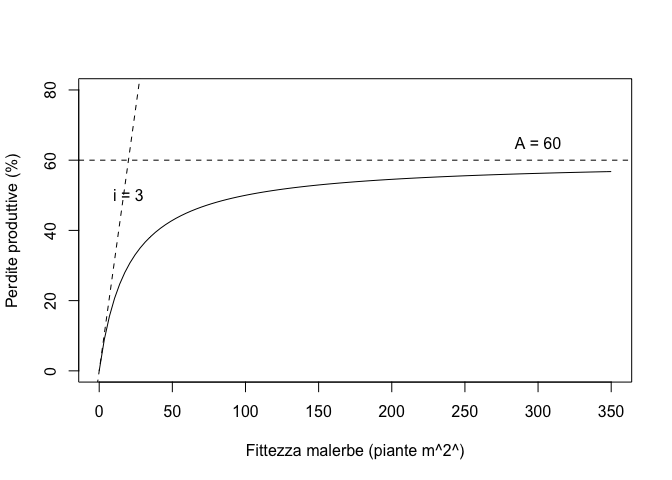
\includegraphics[width=0.9\linewidth]{_main_files/figure-latex/figName25131-1} 

}

\caption{Relazione iperbolica tra fittezza delle piante infestanti e perdite produttive. È  visualizzata la pendenza iniziale (i) e la perdita produttiva massima asintotica (A).}\label{fig:figName25131}
\end{figure}

Normalmente, in campo non vengono determinate le perdite produttive, bensì le produzioni, come nel caso dell'esperimento relativo al dataset d'esempio. Di conseguenza, il modello iperbolico presentato più sopra non è adatto ai nostri dati, in quanto rappresenta una funzione crescente, mentre i nostri dati mostrano una variabile dipendente (produzione) che decresce al crescera della variabile indipendente (fittezza dell piante infestanti). Pertanto, abbiamo due possibilità:

\begin{enumerate}
\def\labelenumi{\arabic{enumi}.}
\tightlist
\item
  modificare il dataset, esprimendo i dati in termini di perdite produttive percentuali;
\item
  modificare il modello, per utilizzare la produzione come variabile dipendente, al posto della perdita produttiva.
\end{enumerate}

La prima strada è più agevole, ma ha un problema importante. Infatti, per calcolare la perdita produttiva percentuale nella parcella \(i\), possiamo utilizzare la seguente equazione:

\[YL_i = \frac{YWF - Y_i}{YWF} \times 100\]

dove \(YWF\) è la produzione nel testimone non infestato e \(Y_i\) è la produzione nella parcella \(i\). Trattandosi di una prova replicata, abbiamo quattro valori di produzione corrispondenti a YWF; quale usiamo? La scelta più logica è quella di utilizzare il valore medio, cioè;

\begin{Shaded}
\begin{Highlighting}[]
\NormalTok{YWF <-}\StringTok{ }\KeywordTok{mean}\NormalTok{(competition}\OperatorTok{$}\NormalTok{Yield[competition}\OperatorTok{$}\NormalTok{Dens}\OperatorTok{==}\DecValTok{0}\NormalTok{])}
\NormalTok{YWF}
\CommentTok{## [1] 30.42637}
\end{Highlighting}
\end{Shaded}

Operando la trasformazione otteniamo una nuova variabile (YL), che possiamo sottoporre a regressione non-lineare, con il modello iperbolico precedentemente indicato. Per ottenere i valori iniziali, possiamo considerare che, con 10 piante per metro quadrato, la perdita produttiva è del 30-35\%. Quindi si può immaginare che la prima pianta infestante aggiunta possa (quella che fa più danni) possa causare perdite produttive del 6-7\% circa. Vediamo inoltre che la perdita produttiva massima osservata è del 70\% circa, quindi possiamo immaginare una perdita produttiva massima asintotica del 75\%.

\begin{Shaded}
\begin{Highlighting}[]
\NormalTok{YL <-}\StringTok{ }\NormalTok{(YWF }\OperatorTok{-}\StringTok{ }\NormalTok{competition}\OperatorTok{$}\NormalTok{Yield)}\OperatorTok{/}\NormalTok{YWF }\OperatorTok{*}\StringTok{ }\DecValTok{100}
\NormalTok{mod1 <-}\StringTok{ }\KeywordTok{nls}\NormalTok{(YL }\OperatorTok{~}\StringTok{ }\NormalTok{i }\OperatorTok{*}\StringTok{ }\NormalTok{Dens }\OperatorTok{/}\StringTok{ }\NormalTok{(}\DecValTok{1} \OperatorTok{+}\StringTok{ }\NormalTok{i }\OperatorTok{*}\StringTok{ }\NormalTok{Dens }\OperatorTok{/}\StringTok{ }\NormalTok{A),}
            \DataTypeTok{start =} \KeywordTok{list}\NormalTok{(}\DataTypeTok{i =} \FloatTok{6.5}\NormalTok{, }\DataTypeTok{A =} \DecValTok{75}\NormalTok{),}
            \DataTypeTok{data =}\NormalTok{ competition)}
\KeywordTok{summary}\NormalTok{(mod1)}
\CommentTok{## }
\CommentTok{## Formula: YL ~ i * Dens/(1 + i * Dens/A)}
\CommentTok{## }
\CommentTok{## Parameters:}
\CommentTok{##   Estimate Std. Error t value Pr(>|t|)    }
\CommentTok{## i    8.207      1.187   6.914 1.93e-08 ***}
\CommentTok{## A   75.049      2.353  31.894  < 2e-16 ***}
\CommentTok{## ---}
\CommentTok{## Signif. codes:  0 '***' 0.001 '**' 0.01 '*' 0.05 '.' 0.1 ' ' 1}
\CommentTok{## }
\CommentTok{## Residual standard error: 6.061 on 42 degrees of freedom}
\CommentTok{## }
\CommentTok{## Number of iterations to convergence: 3 }
\CommentTok{## Achieved convergence tolerance: 7.497e-06}
\end{Highlighting}
\end{Shaded}

Qual è il problema di questo approccio? Se ci facciamo caso, questo modello prevede che, quando la fittezza delle piante infestanti è 0 (testimone non infestato), la perdita produttiva è 0. Di conseguenza la produzione osservata deve essere pari alla media del testimone non infestato. Insomma, abbiamo involontariamente imposto il vincolo YWF = 30.42637, anche se sappiamo che questo vincolo non ha alcuna giustificazione, dato che la media della popolazione da cui le nostre quattro osservazioni non inerbite derivano, difficilmente coincide con la media osservata.

Invece che riorganizzare i dati perché si adattino al modello, potremmo forse tentare di riorganizzare il modello, affinchè si adatti meglio ai dati.

Dalla precedente funzione si ricava che:

\[Y_i = YWF - \frac{YL \times YWF}{100} = YWF\left( {1 - \frac{YL}{100}} \right)\]

che mostra come la produzione in una qualunque parcella (\(Y_i\)) può essere ottenuta in funzione della perdita produttiva e di YWF. Considerando l'equazione precedente e il modello delle perdite produttive, possiamo scrivere:

\[Y_i = YWF\left( {1 - \frac{iD}{100\left( {1 + \frac{iD}{A}} \right)}} \right)\]

Questa equazione consente di utilizzare i dati produttivi osservati come variabile dipendente e di stimare i parametri competitivi \(i\) ed \(A\), insieme alla produzione stimata in asssenza di competizione.

\begin{Shaded}
\begin{Highlighting}[]
\NormalTok{modComp <-}\StringTok{ }\KeywordTok{nls}\NormalTok{(Yield }\OperatorTok{~}\StringTok{ }\NormalTok{YWF }\OperatorTok{*}\StringTok{ }\NormalTok{(}\DecValTok{1} \OperatorTok{-}\StringTok{ }\NormalTok{(i}\OperatorTok{*}\NormalTok{Dens)}\OperatorTok{/}\NormalTok{(}\DecValTok{100} \OperatorTok{*}\StringTok{ }\NormalTok{(}\DecValTok{1} \OperatorTok{+}\StringTok{ }\NormalTok{i }\OperatorTok{*}\StringTok{ }\NormalTok{Dens}\OperatorTok{/}\NormalTok{A))),}
               \KeywordTok{list}\NormalTok{(}\DataTypeTok{YWF =} \FloatTok{30.4}\NormalTok{, }\DataTypeTok{i =} \FloatTok{6.5}\NormalTok{, }\DataTypeTok{A =} \DecValTok{75}\NormalTok{),}
               \DataTypeTok{data=}\NormalTok{competition)}
\KeywordTok{summary}\NormalTok{(modComp)}
\CommentTok{## }
\CommentTok{## Formula: Yield ~ YWF * (1 - (i * Dens)/(100 * (1 + i * Dens/A)))}
\CommentTok{## }
\CommentTok{## Parameters:}
\CommentTok{##     Estimate Std. Error t value Pr(>|t|)    }
\CommentTok{## YWF   30.472      0.930  32.765  < 2e-16 ***}
\CommentTok{## i      8.240      1.387   5.943 5.22e-07 ***}
\CommentTok{## A     75.073      2.422  30.998  < 2e-16 ***}
\CommentTok{## ---}
\CommentTok{## Signif. codes:  0 '***' 0.001 '**' 0.01 '*' 0.05 '.' 0.1 ' ' 1}
\CommentTok{## }
\CommentTok{## Residual standard error: 1.866 on 41 degrees of freedom}
\CommentTok{## }
\CommentTok{## Number of iterations to convergence: 3 }
\CommentTok{## Achieved convergence tolerance: 9.819e-06}
\end{Highlighting}
\end{Shaded}

Vediamo che, in questo caso, la produzione nel testimone non infestato non è più fissata al valor medio osservato, ma è stimata utilizzando tutti i dati sperimentali ed è, pertanto, più precisa.

Pur essendo entrambi gli approcci corretti, il secondo è certamente più elegante e attendibile.

\hypertarget{altre-letture-5}{%
\subsection{Altre letture}\label{altre-letture-5}}

\begin{enumerate}
\def\labelenumi{\arabic{enumi}.}
\tightlist
\item
  Bates, D.M., Watts, D.G., 1988. Nonlinear regression analysis \& its applications. John Wiley \& Sons, Inc., Books.
\item
  Bolker, B.M., 2008. Ecological models and data in R. Princeton University Press, Books.
\item
  Carroll, R.J., Ruppert, D., 1988. Transformation and weighting in regression. Chapman and Hall, Books.
\item
  Ratkowsky, D.A., 1990. Handbook of nonlinear regression models. Marcel Dekker Inc., Books.
\item
  Ritz, C., Streibig, J.C., 2008. Nonlinear regression with R. Springer-Verlag New York Inc., Books.
\end{enumerate}

\hypertarget{appendice-1-breve-introduzione-ad-r}{%
\chapter{Appendice 1: breve introduzione ad R}\label{appendice-1-breve-introduzione-ad-r}}

\hypertarget{cosa-e-r}{%
\section*{Cosa è R?}\label{cosa-e-r}}
\addcontentsline{toc}{section}{Cosa è R?}

R è un software cugino di S-PLUS, con il quale condivide la gran parte delle procedure ed una perfetta compatibilità. Rispetto al cugino più famoso, è completamente freeware (sotto la licenza GNU General Public Licence della Free Software Foundation) ed è nato proprio per mettere a disposizione degli utenti un software gratuito, potente, mantenendo comunque la capacità di lavorare in proprio senza usare software di frodo.

E'uno strumento molto potente, anche da un punto di vista grafico, ma necessita di una certa pratica, in quanto manca di una vera e propria interfaccia grafica (Graphical User Interface: GUI) e, di conseguenza, è spesso necessario scrivere codice.

Inoltre, si tratta di un programma \emph{Open Source}, cioè ognuno può avere accesso al suo codice interno ed, eventualmente, proporne modifiche. Altro vantaggio è che, oltre che un programma, R è anche un linguaggio \emph{object oriented}, che può essere utilizzato dall'utente per creare funzioni personalizzate.

\textbf{Per evitare noiosi errori che possono essere molto comuni per chi è abituato a lavorare in ambiente WINDOWS, è bene precisare subito che R, come tutti i linguaggi di derivazione UNIX, è \emph{case sensitive}, cioè distingue tra lettere maiuscole e lettere minuscole.}

\hypertarget{oggetti-e-assegnazioni}{%
\section*{Oggetti e assegnazioni}\label{oggetti-e-assegnazioni}}
\addcontentsline{toc}{section}{Oggetti e assegnazioni}

\hypertarget{costanti-e-vettori}{%
\subsection*{Costanti e vettori}\label{costanti-e-vettori}}
\addcontentsline{toc}{subsection}{Costanti e vettori}

R lavora con valori, stringhe di caratteri, vettori e matrici, che vengono assegnati alle variabili con opportuni comandi. Ad esempio, il comando:

\begin{Shaded}
\begin{Highlighting}[]
\NormalTok{y  <-}\StringTok{  }\DecValTok{3}
\NormalTok{y}
\CommentTok{## [1] 3}
\end{Highlighting}
\end{Shaded}

assegna il valore 3 alla variabile \emph{y}. Invece il comando:

\begin{Shaded}
\begin{Highlighting}[]
\NormalTok{x  <-}\StringTok{  }\KeywordTok{c}\NormalTok{(}\DecValTok{1}\NormalTok{, }\DecValTok{2}\NormalTok{, }\DecValTok{3}\NormalTok{)}
\NormalTok{x}
\CommentTok{## [1] 1 2 3}
\end{Highlighting}
\end{Shaded}

crea un vettore \emph{x} contenente i numeri 1,2 e 3. Bisogna precisare che il `vettore', in R, non ha alcun legame con la fisica o l'algebra, ed è semplicemente una collezione di numeri (o strighe) consecutivi.

Gli elementi dei vettori possono essere richiamati con il relativo indice tra parentesi quadre. Ad esempio, il secondo elemento di `x' può essere richiamato come:

\begin{Shaded}
\begin{Highlighting}[]
\NormalTok{x[}\DecValTok{2}\NormalTok{]}
\CommentTok{## [1] 2}
\end{Highlighting}
\end{Shaded}

I vettori possono essere numerici, oppure a stringa, cioè possono contenere caratteri alfanumerici. Ad esempio, nel codice sottostante abbiamo creato un vettore contenente nomi di persona.

\begin{Shaded}
\begin{Highlighting}[]
\NormalTok{nomi <-}\StringTok{ }\KeywordTok{c}\NormalTok{(}\StringTok{"Andrea"}\NormalTok{, }\StringTok{"Luca"}\NormalTok{, }\StringTok{"Sandro"}\NormalTok{, }\StringTok{"Mario"}\NormalTok{)}
\NormalTok{nomi}
\CommentTok{## [1] "Andrea" "Luca"   "Sandro" "Mario"}
\end{Highlighting}
\end{Shaded}

Un oggetto leggermente diverso è il fattore sperimentale (`factor'), che contiene caratteri alfanumerici (come nel caso precedente), ma rappresenta una variabile qualitativa di classificazione in categorie.

\begin{Shaded}
\begin{Highlighting}[]
\NormalTok{classe <-}\StringTok{ }\KeywordTok{factor}\NormalTok{(}\KeywordTok{c}\NormalTok{(}\StringTok{"Uomo"}\NormalTok{, }\StringTok{"Uomo"}\NormalTok{, }\StringTok{"Donna"}\NormalTok{, }\StringTok{"Donna"}\NormalTok{, }\StringTok{"Donna"}\NormalTok{))}
\NormalTok{classe}
\CommentTok{## [1] Uomo  Uomo  Donna Donna Donna}
\CommentTok{## Levels: Donna Uomo}
\end{Highlighting}
\end{Shaded}

\hypertarget{matrici}{%
\subsection*{Matrici}\label{matrici}}
\addcontentsline{toc}{subsection}{Matrici}

Oltre ai vettori, in R possiamo definire le matrici. Ad esempio il comando:

\begin{Shaded}
\begin{Highlighting}[]
\NormalTok{z  <-}\StringTok{  }\KeywordTok{matrix}\NormalTok{(}\KeywordTok{c}\NormalTok{(}\DecValTok{1}\NormalTok{, }\DecValTok{2}\NormalTok{, }\DecValTok{3}\NormalTok{, }\DecValTok{4}\NormalTok{, }\DecValTok{5}\NormalTok{, }\DecValTok{6}\NormalTok{, }\DecValTok{7}\NormalTok{, }\DecValTok{8}\NormalTok{), }\DecValTok{2}\NormalTok{, }\DecValTok{4}\NormalTok{, }
              \DataTypeTok{byrow=}\OtherTok{TRUE}\NormalTok{)}
\end{Highlighting}
\end{Shaded}

crea una matrice \emph{z} a 2 righe e 4 colonne, contenente i numeri da 1 a 8. La matrice viene riempita per riga.

Come già mostrato, per visualizzare il contenuto di una variabile basta digitare il nome della variabile. Ad esempio:

\begin{Shaded}
\begin{Highlighting}[]
\NormalTok{z}
\CommentTok{##      [,1] [,2] [,3] [,4]}
\CommentTok{## [1,]    1    2    3    4}
\CommentTok{## [2,]    5    6    7    8}
\end{Highlighting}
\end{Shaded}

Gli elementi di una matrice possono essere richiamati con gli indici e, dato che vi sono due dimensioni (righe e colonne), abbiamo bisogno di due indici, separati da virgole:

\begin{Shaded}
\begin{Highlighting}[]
\NormalTok{z[}\DecValTok{1}\NormalTok{,}\DecValTok{3}\NormalTok{]}
\CommentTok{## [1] 3}
\end{Highlighting}
\end{Shaded}

\hypertarget{dataframe}{%
\subsection*{Dataframe}\label{dataframe}}
\addcontentsline{toc}{subsection}{Dataframe}

Oltre a vettori e matrici, in R esiste un altro importante oggetto, cioè il \emph{dataframe}, costituito da una tabella di dati con una o più colonne di variabili e una o più righe di dati. A differenza della matrice, il dataframe può essere utilizzato per memorizzare variabili di diverso tipo (numeri e caratteri). Un dataframe può essere creato unendo più vettori, come nell'esempio seguente.

\begin{Shaded}
\begin{Highlighting}[]
\NormalTok{parcelle  <-}\StringTok{  }\KeywordTok{c}\NormalTok{(}\DecValTok{1}\NormalTok{, }\DecValTok{2}\NormalTok{, }\DecValTok{3}\NormalTok{, }\DecValTok{4}\NormalTok{, }\DecValTok{5}\NormalTok{, }\DecValTok{6}\NormalTok{)}
\NormalTok{tesi  <-}\StringTok{  }\KeywordTok{factor}\NormalTok{(}\KeywordTok{c}\NormalTok{(}\StringTok{"A"}\NormalTok{, }\StringTok{"A"}\NormalTok{, }\StringTok{"B"}\NormalTok{, }\StringTok{"B"}\NormalTok{, }\StringTok{"C"}\NormalTok{, }\StringTok{"C"}\NormalTok{))}
\NormalTok{dati  <-}\StringTok{  }\KeywordTok{c}\NormalTok{(}\DecValTok{12}\NormalTok{, }\DecValTok{15}\NormalTok{, }\DecValTok{16}\NormalTok{, }\DecValTok{13}\NormalTok{, }\DecValTok{11}\NormalTok{, }\DecValTok{19}\NormalTok{)}
\NormalTok{tabella  <-}\StringTok{  }\KeywordTok{data.frame}\NormalTok{(}\StringTok{"Parc"}\NormalTok{=parcelle,}\StringTok{"Tesi"}\NormalTok{=tesi,}\StringTok{"Produzioni"}\NormalTok{=dati)}
\NormalTok{tabella}
\CommentTok{##   Parc Tesi Produzioni}
\CommentTok{## 1    1    A         12}
\CommentTok{## 2    2    A         15}
\CommentTok{## 3    3    B         16}
\CommentTok{## 4    4    B         13}
\CommentTok{## 5    5    C         11}
\CommentTok{## 6    6    C         19}
\end{Highlighting}
\end{Shaded}

Per utilizzare i dati in un dataframe, bisognerà accedere ai singoli vettori colonna che lo costituiscono. Per far questo possiamo utilizzare l'estrattore \emph{\$}:

\begin{Shaded}
\begin{Highlighting}[]
\NormalTok{tabella}\OperatorTok{$}\NormalTok{Parc}
\CommentTok{## [1] 1 2 3 4 5 6}
\end{Highlighting}
\end{Shaded}

oppure possiamo utilizzare gli indici, che come nel caso delle matrici, sono due, uno per le righe e uno per le colonne, separati da virgole:

\begin{Shaded}
\begin{Highlighting}[]
\NormalTok{tabella[}\DecValTok{2}\NormalTok{,}\DecValTok{1}\NormalTok{]}
\CommentTok{## [1] 2}
\end{Highlighting}
\end{Shaded}

\hypertarget{quale-oggetto-sto-utilizzando}{%
\subsection*{Quale oggetto sto utilizzando?}\label{quale-oggetto-sto-utilizzando}}
\addcontentsline{toc}{subsection}{Quale oggetto sto utilizzando?}

Per avere informazioni sulla natura di un oggetto creato in R, posso usare la funzione \texttt{str()}, come nell'esempio seguente:

\begin{Shaded}
\begin{Highlighting}[]
\KeywordTok{str}\NormalTok{(tabella)}
\CommentTok{## 'data.frame':    6 obs. of  3 variables:}
\CommentTok{##  $ Parc      : num  1 2 3 4 5 6}
\CommentTok{##  $ Tesi      : Factor w/ 3 levels "A","B","C": 1 1 2 2 3 3}
\CommentTok{##  $ Produzioni: num  12 15 16 13 11 19}
\end{Highlighting}
\end{Shaded}

Vediamo infatti che R ci informa che l'oggetto `tabella' è in realtà un dataframe composto da tre colonne, di cui la prima e la terza sono numeriche, mentre la seconda è una variabile qualitativa (fattore).

Inoltre, esiste un'altra funzione molto comune in R, che permette di ottenere informazione riassuntive su un oggetto. Si tratta della funzione `summary()', che fornisce un output diverso a seconda dell'oggetto che le viene passato come argomento:

\begin{Shaded}
\begin{Highlighting}[]
\KeywordTok{summary}\NormalTok{(nomi)}
\CommentTok{##    Length     Class      Mode }
\CommentTok{##         4 character character}
\KeywordTok{summary}\NormalTok{(classe)}
\CommentTok{## Donna  Uomo }
\CommentTok{##     3     2}
\KeywordTok{summary}\NormalTok{(tabella)}
\CommentTok{##       Parc      Tesi    Produzioni   }
\CommentTok{##  Min.   :1.00   A:2   Min.   :11.00  }
\CommentTok{##  1st Qu.:2.25   B:2   1st Qu.:12.25  }
\CommentTok{##  Median :3.50   C:2   Median :14.00  }
\CommentTok{##  Mean   :3.50         Mean   :14.33  }
\CommentTok{##  3rd Qu.:4.75         3rd Qu.:15.75  }
\CommentTok{##  Max.   :6.00         Max.   :19.00}
\end{Highlighting}
\end{Shaded}

\hypertarget{operazioni-ed-operatori}{%
\section*{Operazioni ed operatori}\label{operazioni-ed-operatori}}
\addcontentsline{toc}{section}{Operazioni ed operatori}

Gli oggetti numerici possono essere manipolati anche con opportune operazioni algebriche, che si eseguono utilizzando i normali operatori (+, -, *, /). Ad esempio:

\begin{Shaded}
\begin{Highlighting}[]
\NormalTok{f  <-}\StringTok{  }\DecValTok{2} \OperatorTok{*}\StringTok{ }\NormalTok{y}
\NormalTok{f}
\CommentTok{## [1] 6}
\end{Highlighting}
\end{Shaded}

\hypertarget{funzioni-ed-argomenti}{%
\section*{Funzioni ed argomenti}\label{funzioni-ed-argomenti}}
\addcontentsline{toc}{section}{Funzioni ed argomenti}

Per eseguire operazioni particolari si utilizzano, in genere, le funzioni. Una funzione è richiamata con un nome ed uno o più argomenti. Ad esempio, il comando:

\begin{Shaded}
\begin{Highlighting}[]
\KeywordTok{log}\NormalTok{(}\DecValTok{5}\NormalTok{)}
\CommentTok{## [1] 1.609438}
\end{Highlighting}
\end{Shaded}

Calcola il logaritmo naturale di 5 e richiede un solo argomento, cioè il numero di cui calcolare il logaritmo. Al contrario, il comando:

\begin{Shaded}
\begin{Highlighting}[]
\KeywordTok{log}\NormalTok{(}\DecValTok{100}\NormalTok{, }\DecValTok{2}\NormalTok{)}
\CommentTok{## [1] 6.643856}
\end{Highlighting}
\end{Shaded}

Calcola il logaritmo in base 2 di 100 e richiede due argomenti, cioè il numero di cui calcolare il logaritmo e la base del logaritmo. Quando sono necessari due o più argomenti essi debbono essere messi nell'ordine esatto (in questo caso prima il numero poi la base) oppure debbono essere utilizzati i riferimenti corretti. Ad esempio, i due comandi:

\begin{Shaded}
\begin{Highlighting}[]
\KeywordTok{log}\NormalTok{(}\DecValTok{100}\NormalTok{, }\DataTypeTok{base=}\DecValTok{2}\NormalTok{)}
\CommentTok{## [1] 6.643856}
\KeywordTok{log}\NormalTok{(}\DataTypeTok{base=}\DecValTok{2}\NormalTok{, }\DecValTok{100}\NormalTok{)}
\CommentTok{## [1] 6.643856}
\end{Highlighting}
\end{Shaded}

restituiscono lo stesso risultato, al contrario dei due comandi seguenti:

\begin{Shaded}
\begin{Highlighting}[]
\KeywordTok{log}\NormalTok{(}\DecValTok{100}\NormalTok{, }\DecValTok{2}\NormalTok{)}
\CommentTok{## [1] 6.643856}
\KeywordTok{log}\NormalTok{(}\DecValTok{2}\NormalTok{, }\DecValTok{100}\NormalTok{)}
\CommentTok{## [1] 0.150515}
\end{Highlighting}
\end{Shaded}

\hypertarget{consigli-per-limmissione-di-dati-sperimentali}{%
\section*{Consigli per l'immissione di dati sperimentali}\label{consigli-per-limmissione-di-dati-sperimentali}}
\addcontentsline{toc}{section}{Consigli per l'immissione di dati sperimentali}

I dati delle prove sperimentali si possono o importare in R da altri software (ad esempio Excel) oppue si possono digitare direttamente in R. In quest'ultimo caso, in genere, si crea un vettore per ogni colonna di dati e, successivamente, si riuniscono i vettori in un dataframe, che viene poi salvato nel workspace, come vedremo in seguito.

\hypertarget{immissione-manuale-di-dati}{%
\subsection*{Immissione manuale di dati}\label{immissione-manuale-di-dati}}
\addcontentsline{toc}{subsection}{Immissione manuale di dati}

L'immissione dei dati in R (e quindi la creazione di vettori) può essere velocizzata utilizzando la funzione \texttt{scan()}, separando i dati con INVIO (questo è comodo perchè ci permette di lavorare senza abbandonare il tastierino numerico!). L'immissione termina quando si digita un INVIO a vuoto.

\begin{verbatim}
dati <- scan()
1: 12
2: 14
3: 16
4: 18
5: 20
6:
Read 5 items
dati
[1] 12 14 16 18 20
\end{verbatim}

La stessa funzione può essere anche utilizzata per immettere comodamente stringhe di caratteri, con un opportuno impiego dell'argomento \texttt{what}. In questo caso è possibile omettere le virgolette.

\begin{verbatim}
tesi  <-  scan(what = "character")
1: aurelio
2: aurelio
3: aurelio
4: claudio
5: claudio
6: claudio
7: latino
8: latino
9: latino
10: 
Read 9 items
tesi
[1] "aurelio" "aurelio" "aurelio" "claudio" 
    "claudio" "claudio" "latino"  "latino"  "latino" 
>
\end{verbatim}

\hypertarget{immissione-di-numeri-progressivi}{%
\subsection*{Immissione di numeri progressivi}\label{immissione-di-numeri-progressivi}}
\addcontentsline{toc}{subsection}{Immissione di numeri progressivi}

Per creare una serie progressiva, si può utilizzare il comando \texttt{seq(n,m,by=step)} che genera una sequenza da \(n\) a \(m\) con passo pari a \(step\).

\begin{Shaded}
\begin{Highlighting}[]
\KeywordTok{options}\NormalTok{(}\DataTypeTok{width =} \DecValTok{55}\NormalTok{)}
\NormalTok{parcelle  <-}\StringTok{  }\KeywordTok{seq}\NormalTok{(}\DecValTok{1}\NormalTok{,}\DecValTok{50}\NormalTok{,}\DecValTok{1}\NormalTok{)}
\NormalTok{parcelle}
\CommentTok{##  [1]  1  2  3  4  5  6  7  8  9 10 11 12 13 14 15 16 17}
\CommentTok{## [18] 18 19 20 21 22 23 24 25 26 27 28 29 30 31 32 33 34}
\CommentTok{## [35] 35 36 37 38 39 40 41 42 43 44 45 46 47 48 49 50}
\end{Highlighting}
\end{Shaded}

\hypertarget{immissione-dei-codici-delle-tesi-e-dei-blocchi}{%
\subsection*{Immissione dei codici delle tesi e dei blocchi}\label{immissione-dei-codici-delle-tesi-e-dei-blocchi}}
\addcontentsline{toc}{subsection}{Immissione dei codici delle tesi e dei blocchi}

A volte i codici delle tesi sono sequenze ripetute di stringhe. Ad esempio, i primi quattro dati potrebbero essere riferiti alla varietà BAIO, i secondi quattro alla varietà DUILIO, i successivi quattro alla varietà PLINIO. Per creare velocemente questo vettore, possiamo utilizzare la funzione \texttt{rep()}, in questo modo.

\begin{Shaded}
\begin{Highlighting}[]
\KeywordTok{options}\NormalTok{(}\DataTypeTok{width =} \DecValTok{55}\NormalTok{)}
\NormalTok{tesi  <-}\StringTok{  }\KeywordTok{factor}\NormalTok{(}\KeywordTok{c}\NormalTok{(}\StringTok{"BAIO"}\NormalTok{, }\StringTok{"DUILIO"}\NormalTok{, }\StringTok{"PLINIO"}\NormalTok{))}
\NormalTok{tesi}
\CommentTok{## [1] BAIO   DUILIO PLINIO}
\CommentTok{## Levels: BAIO DUILIO PLINIO}
\NormalTok{tesi  <-}\StringTok{  }\KeywordTok{rep}\NormalTok{(tesi,}\DataTypeTok{each=}\DecValTok{4}\NormalTok{)}
\NormalTok{tesi}
\CommentTok{##  [1] BAIO   BAIO   BAIO   BAIO   DUILIO DUILIO DUILIO}
\CommentTok{##  [8] DUILIO PLINIO PLINIO PLINIO PLINIO}
\CommentTok{## Levels: BAIO DUILIO PLINIO}
\end{Highlighting}
\end{Shaded}

Notare l'uso della funzione \texttt{factor()} per creare un vettore di dati qualitativi (fattore).
Allo stesso modo, per immettere i codici dei blocchi possiamo utilizzare la stessa funzione in un modo diverso. Ammettiamo infatti che i quattro valori di ogni tesi appartengano rispettivamente ai quattro blocchi; si opera quindi in questo modo.

\begin{Shaded}
\begin{Highlighting}[]
\NormalTok{tesi  <-}\StringTok{  }\NormalTok{(}\KeywordTok{c}\NormalTok{ (}\DecValTok{1}\NormalTok{, }\DecValTok{2}\NormalTok{, }\DecValTok{3}\NormalTok{, }\DecValTok{4}\NormalTok{))}
\NormalTok{tesi <-}\StringTok{ }\KeywordTok{rep}\NormalTok{(tesi, }\DataTypeTok{times=}\DecValTok{3}\NormalTok{)}
\NormalTok{tesi}
\CommentTok{##  [1] 1 2 3 4 1 2 3 4 1 2 3 4}
\end{Highlighting}
\end{Shaded}

\hypertarget{leggere-e-salvare-dati-esterni}{%
\subsection*{Leggere e salvare dati esterni}\label{leggere-e-salvare-dati-esterni}}
\addcontentsline{toc}{subsection}{Leggere e salvare dati esterni}

Oltre che immessi da tastiera, i dati possono essere importati in R da files esterni, Inoltre, gli oggetti di R creati nel corso di una sessione possono essere memorizzati su files esterni. Partiamo dal presupposto di aver creato (come frequentemente avviene) il nostro database con EXCEL e di volerlo importare in R nel DATAFRAME \emph{dati}.

Creiamo in EXCEL la tabella riportata di seguito, che si riferisce a 20 piante di mais.

\begin{longtable}[]{@{}lll@{}}
\toprule
Pianta & Var & Altezza\tabularnewline
\midrule
\endhead
1 & N & 172\tabularnewline
2 & S & 154\tabularnewline
3 & V & 150\tabularnewline
4 & V & 188\tabularnewline
5 & C & 162\tabularnewline
6 & N & 145\tabularnewline
7 & C & 157\tabularnewline
8 & C & 178\tabularnewline
9 & V & 175\tabularnewline
10 & N & 158\tabularnewline
11 & N & 153\tabularnewline
12 & N & 191\tabularnewline
13 & S & 174\tabularnewline
14 & C & 141\tabularnewline
15 & N & 165\tabularnewline
16 & C & 163\tabularnewline
17 & V & 148\tabularnewline
18 & S & 152\tabularnewline
19 & C & 169\tabularnewline
20 & C & 185\tabularnewline
\bottomrule
\end{longtable}

La procedura è la seguente:

\begin{enumerate}
\def\labelenumi{\arabic{enumi}.}
\tightlist
\item
  salviamo questa tabella nel file di testo: \emph{comma delineated} `import.csv'. Per far questo scegliere `Menù - File - Salva con nome'. Scegliere un nome per il file ed indicare: 'Tipo file = CSV (delimitato dal separatore di elenco) (*.csv). Salvare quindi il file in una directory prescelta.
\item
  Avviare una sessione R, cambiare la directory predefinita del sistema, scegliendo, con il menu File - Change Directory, la cartella nella quale abbiamo memorizzato il file di importazione.
\item
  Leggere il file di testo in un dataframe, con il seguente comando:
\end{enumerate}

\begin{verbatim}
setwd("myWorkingDir")
dati  <-  read.csv("import.csv", header=TRUE)
\end{verbatim}

Il comando appena descritto ha successo per file CSV creati con la versione inglese di Windows, caratterizzati dal punto come separatore decimale e dalla virgola come separatore di elenco. Se invece il computer fosse settato all'italiana, con la virgola come separatore decimale e il punto e virgola come separatore di elenco, allora si potrebbe utilizzare la funzione \texttt{read.csv2()} (stessa sintassi). Con questi due comandi, in R viene creato un dataframe di nome dati, contenente le tre colonne della tabella `import.csv' appena creata, comprese le intestazioni di colonna.

I dati contenuti in un dataframe o in qualunque altro oggetto possono essere salvati in un file esterno (in formato R binario):

\begin{verbatim}
save(file="dati1.rda", dati)
\end{verbatim}

ed eventualmente ricaricati:

\begin{verbatim}
load("dati1.rda")
\end{verbatim}

Per scrivere in un file di testo (in questo caso \emph{comma delineated}, ma il separatore di elenco può essere modificato secondo le nostre esigenze con l'argomento \texttt{sep}) si utilizza il seguente comando:

\begin{verbatim}
write.table(dati, "residui.csv", row.names=FALSE, 
              col.names=TRUE, sep=",")
\end{verbatim}

\hypertarget{alcune-operazioni-comuni-sul-dataset}{%
\section*{Alcune operazioni comuni sul dataset}\label{alcune-operazioni-comuni-sul-dataset}}
\addcontentsline{toc}{section}{Alcune operazioni comuni sul dataset}

\hypertarget{selezionare-un-subset-di-dati}{%
\subsection*{Selezionare un subset di dati}\label{selezionare-un-subset-di-dati}}
\addcontentsline{toc}{subsection}{Selezionare un subset di dati}

E' possibile estrarre da un dataframe un subset di dati utilizzando la funzione:

\begin{verbatim}
subset(dataframe, condizione)
\end{verbatim}

Ad esempio, se consideriamo il dataframe tabella creato in precedenza, è possibile selezionare tutte le righe relative alle Tesi A e C come segue:

\begin{Shaded}
\begin{Highlighting}[]
\NormalTok{tabella2  <-}\StringTok{  }\KeywordTok{subset}\NormalTok{(tabella, Tesi }\OperatorTok{==}\StringTok{ "A"} \OperatorTok{|}\StringTok{ }\NormalTok{Tesi }\OperatorTok{==}\StringTok{ "C"}\NormalTok{)}
\NormalTok{tabella2}
\CommentTok{##   Parc Tesi Produzioni}
\CommentTok{## 1    1    A         12}
\CommentTok{## 2    2    A         15}
\CommentTok{## 5    5    C         11}
\CommentTok{## 6    6    C         19}
\end{Highlighting}
\end{Shaded}

Notare il carattere ``\textbar{}'' che esprime la condizione logica OR. La condizione logica AND si esprime con il carattere ``\&''. L'esempio seguente isola i record in cui le varietà sono A o C e, contemporaneamente, la produzione è minore di 19.

\begin{Shaded}
\begin{Highlighting}[]
\NormalTok{tabella3  <-}\StringTok{  }\KeywordTok{subset}\NormalTok{(tabella, Tesi }\OperatorTok{==}\StringTok{ "A"} \OperatorTok{|}\StringTok{ }\NormalTok{Tesi }\OperatorTok{==}\StringTok{ "C"} \OperatorTok{&}\StringTok{ }
\StringTok{                       }\NormalTok{Produzioni }\OperatorTok{<}\StringTok{ }\DecValTok{19}\NormalTok{)}
\NormalTok{tabella3}
\CommentTok{##   Parc Tesi Produzioni}
\CommentTok{## 1    1    A         12}
\CommentTok{## 2    2    A         15}
\CommentTok{## 5    5    C         11}
\end{Highlighting}
\end{Shaded}

\hypertarget{ordinare-un-vettore-o-un-dataframe}{%
\subsection*{Ordinare un vettore o un dataframe}\label{ordinare-un-vettore-o-un-dataframe}}
\addcontentsline{toc}{subsection}{Ordinare un vettore o un dataframe}

Un vettore (numerico o carattere) può essere ordinato con il comando \texttt{sort}:

\begin{Shaded}
\begin{Highlighting}[]
\NormalTok{y  <-}\StringTok{  }\KeywordTok{c}\NormalTok{(}\DecValTok{12}\NormalTok{, }\DecValTok{15}\NormalTok{, }\DecValTok{11}\NormalTok{, }\DecValTok{17}\NormalTok{, }\DecValTok{12}\NormalTok{, }\DecValTok{8}\NormalTok{, }\DecValTok{7}\NormalTok{, }\DecValTok{15}\NormalTok{)}
\KeywordTok{sort}\NormalTok{(y, }\DataTypeTok{decreasing =} \OtherTok{FALSE}\NormalTok{)}
\CommentTok{## [1]  7  8 11 12 12 15 15 17}
\NormalTok{z  <-}\StringTok{  }\KeywordTok{c}\NormalTok{(}\StringTok{"A"}\NormalTok{, }\StringTok{"C"}\NormalTok{, }\StringTok{"D"}\NormalTok{, }\StringTok{"B"}\NormalTok{, }\StringTok{"F"}\NormalTok{, }\StringTok{"L"}\NormalTok{, }\StringTok{"M"}\NormalTok{, }\StringTok{"E"}\NormalTok{)}
\KeywordTok{sort}\NormalTok{(z, }\DataTypeTok{decreasing =} \OtherTok{TRUE}\NormalTok{)}
\CommentTok{## [1] "M" "L" "F" "E" "D" "C" "B" "A"}
\end{Highlighting}
\end{Shaded}

Un dataframe può essere invece ordinato con il comando \texttt{order()}, facendo attenzione al segno meno utilizzabile per l'ordinamento decrescente.

\begin{verbatim}
dataset[order(dataset$z, dataset$y), ]
dataset[order(dataset$z, -dataset$y), ]
\end{verbatim}

\hypertarget{workspace}{%
\section*{Workspace}\label{workspace}}
\addcontentsline{toc}{section}{Workspace}

Gli oggetti creati durante una sessione di lavoro vengono memorizzati nel cosiddetto workspace. Per il salvataggio del workspace nella directory corrente si usa il menu (File/Save Workspace) oppure il comando:

\begin{verbatim}
save.image('nomefile.RData')
\end{verbatim}

Il contenuto del workspace viene visualizzato con:

\begin{verbatim}
ls()
\end{verbatim}

Il workspace viene richiamato da menu (File/Open Workspace) oppure con il comando:

\begin{verbatim}
load('nomefile.RData')
\end{verbatim}

Per un lavoro efficiente in R è bene tenere il workspace molto pulito, eliminando gli oggetti non necessari. La completa eliminazione degli oggetti nel workspace si esegue con:

\begin{verbatim}
rm(list=ls())
\end{verbatim}

Uno o più oggetti specifici possono essere eliminati con:

\begin{verbatim}
rm(oggetto1, oggetto2, .....)
\end{verbatim}

Gli oggetti possono anche essere richiamati in base alla loro posizione; ad esempio il comando:

\begin{verbatim}
rm(list=ls()[3:4])
\end{verbatim}

elimina il terzo e il quarto oggetto dal workspace.

Un comando particolarmente utile è il seguente:

\begin{verbatim}
rm(list=ls()[ls()!="oggetto1"])
\end{verbatim}

che permette di eliminare dal workspace ogni oggetto meno ``oggetto1''. Si possono utilizzare anche clausole logiche più articolate come la seguente:

\begin{verbatim}
rm(list=ls()[ls()!="oggetto1" & ls()!="oggetto2"])
\end{verbatim}

che elimina tutto meno ``oggetto1'' e ``oggetto2''.

\hypertarget{script-o-programmi}{%
\section*{Script o programmi}\label{script-o-programmi}}
\addcontentsline{toc}{section}{Script o programmi}

Come è possibile memorizzare dati e workspace, è anche possibile creare uno script (procedura, funzione\ldots{}) da memorizzare e richiamare in seguito. Nel caso più semplice è possibile scrivere comandi in un semplice editor di testo e salvarli in un file con estensione `.r'. I comandi possono poi essere riutilizzati per semplice copia ed incolla sulla console, opppure, nel caso in cui si utilizzi Rstudio (FILE -\(>\) APRI SCRIPT o NUOVO SCRIPT) selezionando il comando (o i comandi) da inviare alla console e premendo la combinazione CTRL + INVIO.

Lavorare con scripts è molto comodo e consigliabile perchè non si deve partire da zero ad ogni sessione, ma è sufficiente correggere i comandi digitati in sessioni precedenti.

Oltre agli script, è possibile creare funzioni personalizzate fino ad arrivare a veri e propri programmi (packages). Immaginiamo ad esempio di voler scrivere una funzione che, dato il valore della produzione rilevata in una parcella di orzo di 20 \$ m\^{}2 \$ (in kg) e la sua umidità percentuale, calcoli automaticamente il valore della
produzione secca in kg/ha. La funzione che dobbiamo implementare è:

\[
PS = PU \cdot \frac{100 - U}{100} \cdot \frac{10000}{20}
\]

ove PS è la produzione secca in kg/ha e PU è la produzione all'umidità U in kg per 20 \$ m\^{}2 \$.

Scriveremo un file di testo (ad esempio con il \emph{Block notes} o con l'editor interno ad R):

\begin{verbatim}
PS  <-  function(PU, U) {
  PU*((100-U)/100)*(10000/20)
}
\end{verbatim}

Notare l'uso delle parentesi graffe. Salveremo il file di testo con il nome (ad esempio) ``prova.r''.

Aprendo una nuova sessione in R, possiamo ricaricare in memoria il file di programma (FILE - SORGENTE CODICE R, oppure da console, con il comando:

\begin{verbatim}
source('prova.r')
\end{verbatim}

A differenza di quanto avviene con uno script, i comandi memorizzati nella funzione non vengono eseguiti, ma la funzione `PS' diviene disponibile nel workspace e può essere utilizzata nel modo seguente:

\begin{verbatim}
PS(20,85)
\end{verbatim}

\hypertarget{interrogazione-di-oggetti}{%
\section*{Interrogazione di oggetti}\label{interrogazione-di-oggetti}}
\addcontentsline{toc}{section}{Interrogazione di oggetti}

A differenza di altri linguaggi statistici come SAS o SPSS, R immagazzina i risultati delle analisi negli oggetti, mostrando un output video piuttosto minimale. Per ottenere informazioni è necessario interrogare opportunamente gli oggetti che al loro interno possono contenere altri oggetti da cui recuperare le informazioni interessanti. Gli oggetti che contengono altri oggetti sono detti
\textbf{liste}.

Ad esempio, se vogliamo calcolare autovettori ed autovalori di una
matrice, utilizziamo la funzione `eigen'. Questa funzione restituisce una lista di oggetti, che al suo interno contiene i due oggetti values (autovalori) e vectors (autovettori). Per recuperare l'uno o l'altro dei due risultati (autovettori o autovalori) si usa l'operatore di concatenamento (detto anche estrattore) \$.

\begin{Shaded}
\begin{Highlighting}[]
\NormalTok{matrice  <-}\StringTok{  }\KeywordTok{matrix}\NormalTok{(}\KeywordTok{c}\NormalTok{(}\DecValTok{2}\NormalTok{,}\DecValTok{1}\NormalTok{,}\DecValTok{3}\NormalTok{,}\DecValTok{4}\NormalTok{),}\DecValTok{2}\NormalTok{,}\DecValTok{2}\NormalTok{)}
\NormalTok{matrice}
\CommentTok{##      [,1] [,2]}
\CommentTok{## [1,]    2    3}
\CommentTok{## [2,]    1    4}
\NormalTok{ev  <-}\StringTok{  }\KeywordTok{eigen}\NormalTok{(matrice)}
\NormalTok{ev}
\CommentTok{## eigen() decomposition}
\CommentTok{## $values}
\CommentTok{## [1] 5 1}
\CommentTok{## }
\CommentTok{## $vectors}
\CommentTok{##            [,1]       [,2]}
\CommentTok{## [1,] -0.7071068 -0.9486833}
\CommentTok{## [2,] -0.7071068  0.3162278}
\NormalTok{ev}\OperatorTok{$}\NormalTok{values}
\CommentTok{## [1] 5 1}
\NormalTok{ev}\OperatorTok{$}\NormalTok{vectors}
\CommentTok{##            [,1]       [,2]}
\CommentTok{## [1,] -0.7071068 -0.9486833}
\CommentTok{## [2,] -0.7071068  0.3162278}
\end{Highlighting}
\end{Shaded}

\hypertarget{altre-funzioni-matriciali}{%
\section*{Altre funzioni matriciali}\label{altre-funzioni-matriciali}}
\addcontentsline{toc}{section}{Altre funzioni matriciali}

Oltre che autovettori ed autovalori di una matrice, R ci permette di gestire altre funzioni di matrice. Se ad esempio abbiamo
le matrici:

\[
Z = \left( {\begin{array}{*{20}c}
   1 & 2  
   2 & 3  
\end{array}} \right)\,\,\,\,\,\,\,Y = \left( {\begin{array}{*{20}c}
   3 & 2  
\end{array}} \right)
\]

queste possono essere caricate in R con i seguenti comandi:

\begin{Shaded}
\begin{Highlighting}[]
\NormalTok{Z  <-}\StringTok{  }\KeywordTok{matrix}\NormalTok{(}\KeywordTok{c}\NormalTok{(}\DecValTok{1}\NormalTok{,}\DecValTok{2}\NormalTok{,}\DecValTok{2}\NormalTok{,}\DecValTok{3}\NormalTok{),}\DecValTok{2}\NormalTok{,}\DecValTok{2}\NormalTok{)}
\NormalTok{Y  <-}\StringTok{  }\KeywordTok{matrix}\NormalTok{(}\KeywordTok{c}\NormalTok{(}\DecValTok{3}\NormalTok{,}\DecValTok{2}\NormalTok{),}\DecValTok{1}\NormalTok{,}\DecValTok{2}\NormalTok{)}
\end{Highlighting}
\end{Shaded}

Possiamo poi ottenere la trasposta di Z con il comando:

\begin{Shaded}
\begin{Highlighting}[]
\KeywordTok{t}\NormalTok{(Z)}
\CommentTok{##      [,1] [,2]}
\CommentTok{## [1,]    1    2}
\CommentTok{## [2,]    2    3}
\end{Highlighting}
\end{Shaded}

Possiamo moltiplicare Y e Z utilizzando l'operatore \%*\%:

\begin{Shaded}
\begin{Highlighting}[]
\NormalTok{Y}\OperatorTok\NormalTok{Z}
\CommentTok{##      [,1] [,2]}
\CommentTok{## [1,]    7   12}
\end{Highlighting}
\end{Shaded}

Possiamo calcolare l'inversa di Z con:

\begin{Shaded}
\begin{Highlighting}[]
\KeywordTok{solve}\NormalTok{(Z)}
\CommentTok{##      [,1] [,2]}
\CommentTok{## [1,]   -3    2}
\CommentTok{## [2,]    2   -1}
\end{Highlighting}
\end{Shaded}

\hypertarget{cenni-sulle-funzionalita-grafiche-in-r}{%
\section*{Cenni sulle funzionalità grafiche in R}\label{cenni-sulle-funzionalita-grafiche-in-r}}
\addcontentsline{toc}{section}{Cenni sulle funzionalità grafiche in R}

R è un linguaggio abbastanza potente e permette di creare grafici interessanti. Ovviamente un trattazione esauriente esula dagli scopi di questo testo, anche se è opportuno dare alcune indicazioni che potrebbero essere utili in seguito.
La funzione più utilizzata per produrre grafici è:

\begin{verbatim}
plot(x,y, type, xlab, ylab, col, lwd, lty...)
\end{verbatim}

ovex ed y sono i vettori con le coordinate dei punti da disegnare. \texttt{Type} rappresenta il tipo di grafico (`'p'' produce un grafico a punti, `'l'' un grafico a linee, `'b'' disegna punti uniti da linee, `'h'' disegna istogrammi), 'Title disegna il titolo del grafico, sub il sottotitolo,xlab e ylab le etichette degli assi, col è il colore dell'oggetto, lwd il suo spessore, lty il tipo di linea e così via.

Per una descrizione più dettagliata si consiglia di consultare la documentazione on line. A titolo di esempio, i comandi mostrati qui sotto producono l'output in Figura \ref{fig:figName231}.

\begin{Shaded}
\begin{Highlighting}[]
\NormalTok{x  <-}\StringTok{  }\KeywordTok{c}\NormalTok{(}\DecValTok{1}\NormalTok{, }\DecValTok{2}\NormalTok{, }\DecValTok{3}\NormalTok{, }\DecValTok{4}\NormalTok{)}
\NormalTok{y  <-}\StringTok{  }\KeywordTok{c}\NormalTok{(}\DecValTok{10}\NormalTok{, }\DecValTok{11}\NormalTok{, }\DecValTok{13}\NormalTok{, }\DecValTok{17}\NormalTok{)}
\KeywordTok{plot}\NormalTok{(x, y, }\DataTypeTok{type =} \StringTok{"p"}\NormalTok{, }\DataTypeTok{col=}\StringTok{"red"}\NormalTok{, }\DataTypeTok{lwd=}\DecValTok{5}\NormalTok{, }\DataTypeTok{xlab=}\StringTok{"Ascissa"}\NormalTok{, }\DataTypeTok{ylab=}\StringTok{"Ordinata"}\NormalTok{)}
\end{Highlighting}
\end{Shaded}

\begin{figure}

{\centering 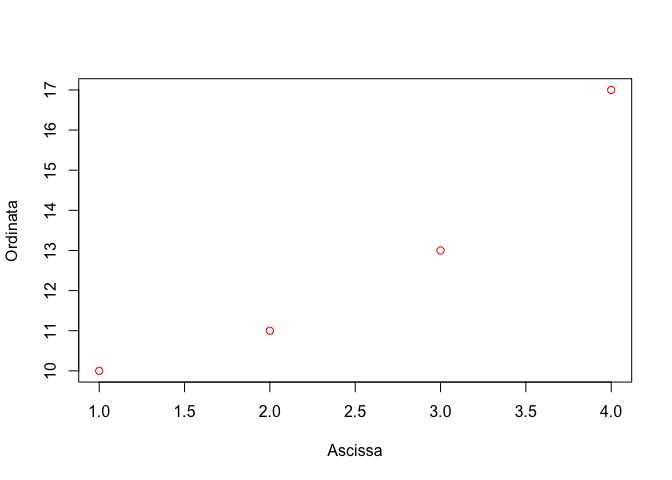
\includegraphics[width=0.9\linewidth]{_main_files/figure-latex/figName231-1} 

}

\caption{Esempio di un semplice grafico a dispersione}\label{fig:figName231}
\end{figure}

Per sovrapporre una seconda serie di dati alla prima possiamo utilizzare la funzione `plot()', come sopra e, successivamente la funzione `points()' per aggiungere la nuova serie. Il risultato è quello mostrato in Figura \ref{fig:figName232}.

\begin{Shaded}
\begin{Highlighting}[]
\NormalTok{y2  <-}\StringTok{  }\KeywordTok{c}\NormalTok{(}\DecValTok{17}\NormalTok{,}\DecValTok{13}\NormalTok{,}\DecValTok{11}\NormalTok{,}\DecValTok{10}\NormalTok{)}
\KeywordTok{plot}\NormalTok{(x, y, }\DataTypeTok{type =} \StringTok{"p"}\NormalTok{, }\DataTypeTok{col=}\StringTok{"red"}\NormalTok{, }\DataTypeTok{lwd=}\DecValTok{5}\NormalTok{, }\DataTypeTok{xlab=}\StringTok{"Ascissa"}\NormalTok{, }\DataTypeTok{ylab=}\StringTok{"Ordinata"}\NormalTok{)}
\KeywordTok{points}\NormalTok{(x, y2, }\DataTypeTok{col=}\StringTok{"blue"}\NormalTok{, }\DataTypeTok{lwd=}\DecValTok{5}\NormalTok{)}
\end{Highlighting}
\end{Shaded}

\begin{figure}

{\centering 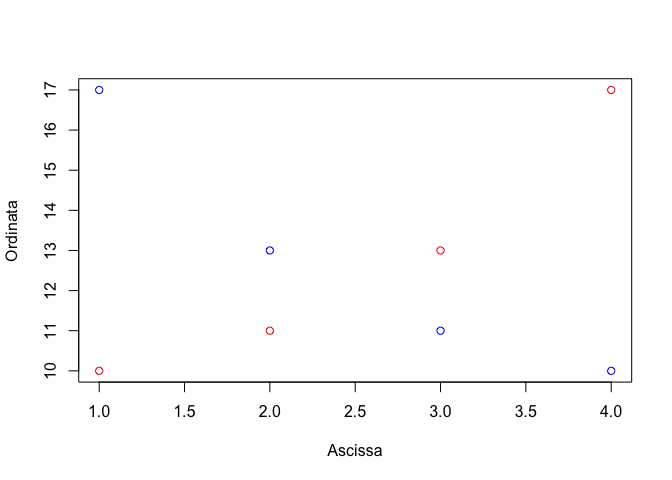
\includegraphics[width=0.9\linewidth]{_main_files/figure-latex/figName232-1} 

}

\caption{Esempio di grafico con due serie di dati}\label{fig:figName232}
\end{figure}

Se avessimo voluto sovrapporre una grafico a linee avremmo utilizzato la funzione `lines()' al posto della funzione `points()', ottenendo l'output in Figura \ref{fig:figName233}.

\begin{Shaded}
\begin{Highlighting}[]
\KeywordTok{plot}\NormalTok{(x, y, }\StringTok{"p"}\NormalTok{, }\DataTypeTok{col=}\StringTok{"red"}\NormalTok{, }\DataTypeTok{lwd=}\DecValTok{5}\NormalTok{,}\DataTypeTok{xlab=}\StringTok{"Ascissa"}\NormalTok{, }\DataTypeTok{ylab=}\StringTok{"Ordinata"}\NormalTok{)}
\KeywordTok{points}\NormalTok{(x, y2, }\DataTypeTok{col=}\StringTok{"blue"}\NormalTok{, }\DataTypeTok{lwd=}\DecValTok{5}\NormalTok{)}
\KeywordTok{lines}\NormalTok{(x, y2, }\DataTypeTok{col=}\StringTok{"blue"}\NormalTok{, }\DataTypeTok{lwd=}\DecValTok{2}\NormalTok{)}
\end{Highlighting}
\end{Shaded}

\begin{figure}

{\centering 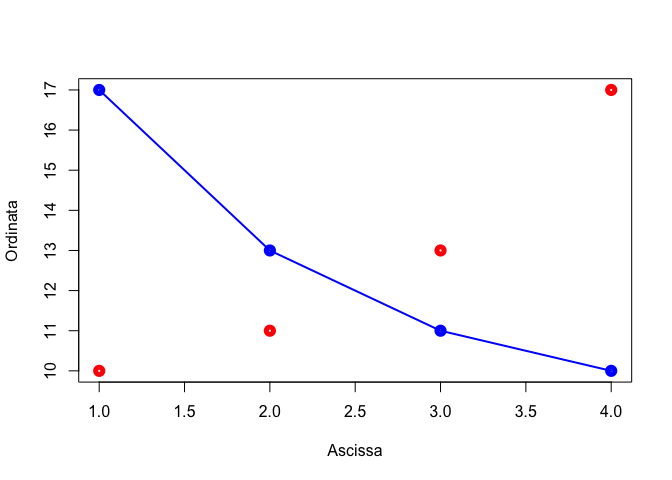
\includegraphics[width=0.9\linewidth]{_main_files/figure-latex/figName233-1} 

}

\caption{Esempio di grafico con due serie di dati, con linee e punti}\label{fig:figName233}
\end{figure}

Per disegnare una curva si può utilizzare la funzione:

\begin{verbatim}
curve(funzione, Xiniziale, Xfinale, add=FALSE/TRUE)
\end{verbatim}

dove l'argomento `add' serve per specificare se la funzione deve essere aggiunta ad un grafico preesistente.

Per aggiungere un titolo ad un grafico possiamo utilizzare la funzione:

\begin{verbatim}
title(main="Titolo")
\end{verbatim}

mentre per aggiungere una legenda utilizziamo la funzione:

\begin{verbatim}
legend(Xcoord, YCoord , legend=c("Punti","X+10"), pch=c(19,-1),
      col=c("Red","Blue"),
      lwd=c(3,3), lty=c(0,3))
\end{verbatim}

ove i vettori indicano, per ogni elemento della legenda, il testo che deve essere riportato (legend), il tipo di simbolo (pch, con -1 che indica nessun simbolo), il colore (col), la larghezza (lwd) e il tipo di linea (lty, con 0 che indica nessuna linea).

Ad esempio, il codice riportato più sotto produce l'output in Figura \ref{fig:figName234}.

\begin{Shaded}
\begin{Highlighting}[]
\KeywordTok{plot}\NormalTok{(x, y, }\StringTok{"p"}\NormalTok{, }\DataTypeTok{col=}\StringTok{"red"}\NormalTok{, }\DataTypeTok{lwd=}\DecValTok{5}\NormalTok{, }\DataTypeTok{xlab=}\StringTok{"Ascissa"}\NormalTok{, }
       \DataTypeTok{ylab =} \StringTok{"Ordinata"}\NormalTok{)}
\KeywordTok{curve}\NormalTok{(}\DecValTok{10}\OperatorTok{+}\NormalTok{x, }\DataTypeTok{add=}\OtherTok{TRUE}\NormalTok{, }\DataTypeTok{lty=}\DecValTok{1}\NormalTok{, }\DataTypeTok{lwd=}\DecValTok{2}\NormalTok{, }\DataTypeTok{col=}\StringTok{"blue"}\NormalTok{)}
\KeywordTok{title}\NormalTok{(}\DataTypeTok{main=}\StringTok{"Grafico di prova"}\NormalTok{)}
\KeywordTok{legend}\NormalTok{(}\DecValTok{1}\NormalTok{,}\DecValTok{17}\NormalTok{, }\DataTypeTok{legend=}\KeywordTok{c}\NormalTok{(}\StringTok{"Punti"}\NormalTok{, }\StringTok{"X+10"}\NormalTok{), }\DataTypeTok{pch=}\KeywordTok{c}\NormalTok{(}\DecValTok{19}\NormalTok{,}\OperatorTok{-}\DecValTok{1}\NormalTok{), }
  \DataTypeTok{col=}\KeywordTok{c}\NormalTok{(}\StringTok{"Red"}\NormalTok{, }\StringTok{"Blue"}\NormalTok{), }\DataTypeTok{lwd=}\KeywordTok{c}\NormalTok{(}\DecValTok{3}\NormalTok{,}\DecValTok{3}\NormalTok{), }\DataTypeTok{lty=}\KeywordTok{c}\NormalTok{(}\DecValTok{0}\NormalTok{,}\DecValTok{1}\NormalTok{))}
\end{Highlighting}
\end{Shaded}

\begin{figure}

{\centering 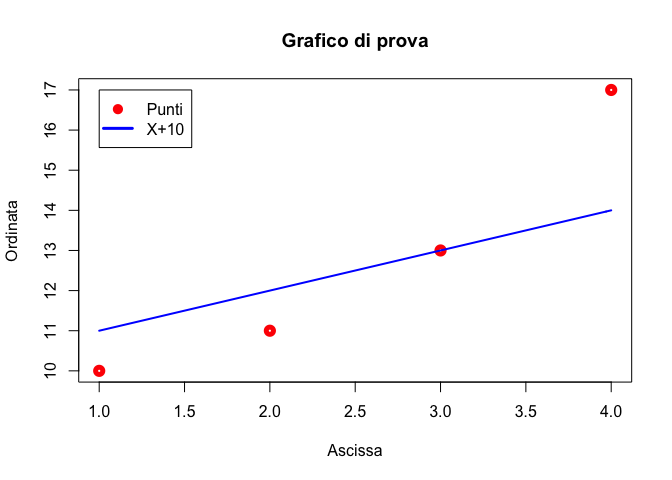
\includegraphics[width=0.9\linewidth]{_main_files/figure-latex/figName234-1} 

}

\caption{Esempio di grafico con titolo e legenda}\label{fig:figName234}
\end{figure}

L'ultima cosa che desideriamo menzionare è la possibilità di disegnare grafici a torta, utilizzando il comando:

\begin{verbatim}
pie(vettoreNumeri, vettoreEtichette, vettoreColori)
\end{verbatim}

Ad esempio il comando sottostante, produce l'output in Figura \ref{fig:figName235}.

\begin{Shaded}
\begin{Highlighting}[]
\KeywordTok{pie}\NormalTok{(}\KeywordTok{c}\NormalTok{(}\DecValTok{20}\NormalTok{,}\DecValTok{30}\NormalTok{,}\DecValTok{50}\NormalTok{),}\DataTypeTok{label=}\KeywordTok{c}\NormalTok{(}\StringTok{"B"}\NormalTok{, }\StringTok{"C"}\NormalTok{),}
        \DataTypeTok{col=}\KeywordTok{c}\NormalTok{(}\StringTok{"blue"}\NormalTok{, }\StringTok{"green"}\NormalTok{, }\StringTok{"red"}\NormalTok{))}
\end{Highlighting}
\end{Shaded}

\begin{figure}

{\centering 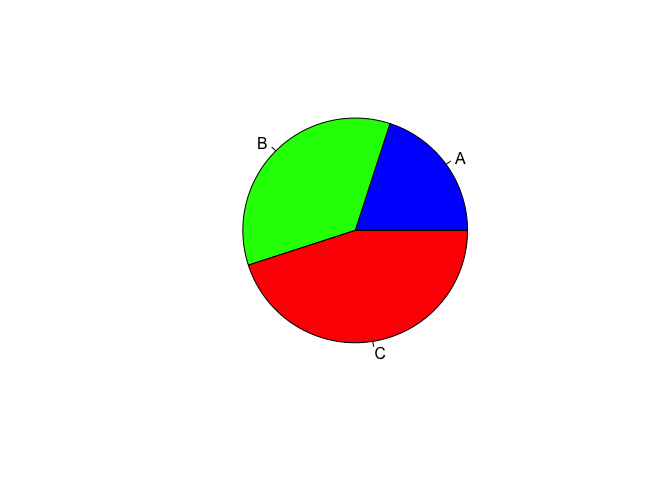
\includegraphics[width=0.45\linewidth]{_main_files/figure-latex/figName235-1} 

}

\caption{Esempio di grafico a torta}\label{fig:figName235}
\end{figure}

\begin{center}\rule{0.5\linewidth}{\linethickness}\end{center}

\hypertarget{per-approfondire-un-po-10}{%
\section{Per approfondire un po'\ldots{}}\label{per-approfondire-un-po-10}}

\begin{enumerate}
\def\labelenumi{\arabic{enumi}.}
\tightlist
\item
  Maindonald J. Using R for Data Analysis and Graphics - Introduction, Examples and Commentary. (PDF, data sets and scripts are available at \href{https://cran.r-project.org/doc/contrib/usingR.pdff}{JM's homepage}.
\item
  Oscar Torres Reina, 2013. Introductio to RStudio (v. 1.3). \href{https://dss.princeton.edu/training/RStudio101.pdf}{This homepage}
\end{enumerate}

\hypertarget{appendice-2-richiami-di-statistica-descrittiva}{%
\chapter{Appendice 2: Richiami di statistica descrittiva}\label{appendice-2-richiami-di-statistica-descrittiva}}

\hypertarget{dati-quantitativi-analisi-chimiche-e-altre-misurazioni-fondamentali}{%
\section*{Dati quantitativi: analisi chimiche e altre misurazioni fondamentali}\label{dati-quantitativi-analisi-chimiche-e-altre-misurazioni-fondamentali}}
\addcontentsline{toc}{section}{Dati quantitativi: analisi chimiche e altre misurazioni fondamentali}

Qualunque esperimento include un processo di misurazione, al termine del quale ci troviamo con un insieme di dati, usualmente definito dataset. Soprattutto se l'insieme è numeroso, è estrememente importante comprenderne le caratteristiche fondamentali e descriverle fedelmente, utilizzando opportune statistiche descrittive. Se le misure rappresentano una quantità, come, ad esempio, il peso, l'altezza, la concentrazione e così via, il dataset deve essere descritto in relazione ad almeno due caratteristiche fondamentali, vale a dire:

\begin{enumerate}
\def\labelenumi{\arabic{enumi}.}
\tightlist
\item
  tendenza centrale (location)
\item
  dispersione (shape)
\end{enumerate}

La tendenza centrale di un dataset è un valore, intorno al quale si collocano tutte le osservazioni, mentre la dispersione misura, in qualche modo, la distanza delle osservazioni tra di loro. Esistono diverse statistiche di tendenza centrale e dispersione; di seguito, descriveremo le più importanti.

\hypertarget{indicatori-di-tendenza-centrale}{%
\subsection*{Indicatori di tendenza centrale}\label{indicatori-di-tendenza-centrale}}
\addcontentsline{toc}{subsection}{Indicatori di tendenza centrale}

L'indicatore di tendenza centrale più diffuso è la \emph{media} aritmetica, che non necessita di particolari spiegazioni: si calcola con R mediante la funzione \texttt{mean()}. Per esempio, carichiamo il dataset `heights' contenuto nel package `aomisc' e calcoliamo la media delle altezze.

\begin{Shaded}
\begin{Highlighting}[]
\KeywordTok{library}\NormalTok{(aomisc)}
\KeywordTok{data}\NormalTok{(heights)}
\KeywordTok{mean}\NormalTok{(heights}\OperatorTok{$}\NormalTok{height)}
\CommentTok{## [1] 164}
\end{Highlighting}
\end{Shaded}

Un altro indicatore di tendenza centrale è la \emph{mediana}, data dal valore che bipartisce i dati in modo da lasciarne metà a sinistra e metà a destra. Se abbiamo una serie di individui ordinati in graduatoria, la mediana è data dall' individuo che occupa il posto (n + 1)/2 o, se gli individui sono in numero pari, dalla media delle due osservazioni centrali. In R, la mediana si calcola con la funzione \texttt{median()}.

\begin{Shaded}
\begin{Highlighting}[]
\KeywordTok{median}\NormalTok{(heights}\OperatorTok{$}\NormalTok{height)}
\CommentTok{## [1] 162.5}
\end{Highlighting}
\end{Shaded}

La mediana è un indicatore più robusto della media: infatti, supponiamo di avere cinque valori:

1 - 4 - 7 - 9 - 10

La media è pari a 6.2, mentre la mediana è pari a 7 (valore centrale). Se cambiano il numero più alto in questo modo:

1 - 4 - 7 - 9 - 100

la media di questi cinque valori sarà 24.2, mentre la mediana sarà sempre pari a 7. Insomma, la mediana non è influenzata da valori estremi (\emph{outliers}), in senso positivo o negativo.

\hypertarget{indicatori-di-dispersione}{%
\subsection*{Indicatori di dispersione}\label{indicatori-di-dispersione}}
\addcontentsline{toc}{subsection}{Indicatori di dispersione}

Gli indicatori di tendenza centrale, da soli, non ci informano su come le unità sperimentali tendono a differire l'una dall'altra: ad esempio una media pari a 100 può essere ottenuta con tre individui che misurano 99, 100 e 101 rispettivamente o con tre individui che misurano 1, 100 e 199. E' evidente che in questo secondo gruppo gli individui sono molto più differenti tra loro (dispersi) che nel primo gruppo.

Pertanto, i risultati di un processo di misurazione non possono essere descritti solo con la media, ma è necessario anche calcolare un indice di variabilità. Tra essi, il più semplice è il \emph{campo di variazione}, che è la differenza tra la misura più bassa e la misura più alta. In realtà, non si tratta di un vero e proprio indice di variabilità, in quanto dipende solo dai termini estremi della distribuzione e non necessariamente cresce al crescere della variabilità degli individui.

Invece del campo di variazione, possiamo utilizzare i cosiddetti \emph{percentili}, che bipartiscono la popolazione di partenza in modo da lasciare una certa quantità di termini alla sua sinistra e la restante quantità alla sua destra. Ad esempio, il primo percentile bipartisce la popolazione in modo da lasciare a sinistra l' 1\% dei termini e alla destra il restante 99\%. Allo stesso modo l' ottantesimo percentile bipartisce la popolazione in modo da lasciare a sinistra l'80\% dei termini e alla destra il restante 20\%. I percentili più utilizzati per descrivere la dispersione di un collettivo sono il 25-esimo e il 75-esimo: se questi sono molto vicini, significa che il 50 \% dei soggetti è compreso in un intervallo piccolo e quindi la variabilità della popolazione è bassa. In R, i percentili si calcolano con il comando sottostante.

\begin{Shaded}
\begin{Highlighting}[]
\KeywordTok{quantile}\NormalTok{(heights}\OperatorTok{$}\NormalTok{height, }\DataTypeTok{probs =} \KeywordTok{c}\NormalTok{(}\FloatTok{0.25}\NormalTok{, }\FloatTok{0.75}\NormalTok{))}
\CommentTok{##    25%    75% }
\CommentTok{## 152.75 174.25}
\end{Highlighting}
\end{Shaded}

A questo proposito, possiamo introdurre il concetto di \emph{boxplot} (grafico Box-Whisker). Si tratta di una scatola che ha per estremi il 25esimo e il 75esimo percentile ed è tagliata da una linea centrale in corrispondenza della mediana. Dalla scatola partono due linee verticali che identificano il valore massimo e il minimo. Se il massimo (o il minimo) distano dalla mediana più di 1.5 volte la differenza tra la mediana stessa e il 75esimo (o 25esimo) percentile, allora le linee verticali si fermano ad un valore pari ad 1.5 volte il 75esimo (o il 25esimo) percentile rispettivamente ed i dati esterni vengono raffigurati come outliers. I boxplot sono solitamente usati per descrivere campioni numerosi nei quali esista un qualche criterio di raggruppamento. In basso abbiamo create tre gruppi con una funzione di estrazione di numeri casuali e li abbiamo rappresentati nel boxplot mostrato in Figura \ref{fig:figName241}.

\begin{Shaded}
\begin{Highlighting}[]
\KeywordTok{set.seed}\NormalTok{(}\DecValTok{1234}\NormalTok{)}
\NormalTok{A <-}\StringTok{ }\KeywordTok{runif}\NormalTok{(}\DecValTok{20}\NormalTok{)}
\NormalTok{B <-}\StringTok{ }\KeywordTok{runif}\NormalTok{(}\DecValTok{20}\NormalTok{)}
\NormalTok{C <-}\StringTok{ }\KeywordTok{runif}\NormalTok{(}\DecValTok{20}\NormalTok{)}
\NormalTok{series <-}\StringTok{ }\KeywordTok{rep}\NormalTok{(}\KeywordTok{c}\NormalTok{(}\StringTok{"A"}\NormalTok{, }\StringTok{"B"}\NormalTok{, }\StringTok{"C"}\NormalTok{), }\DataTypeTok{each =} \DecValTok{20}\NormalTok{)}
\NormalTok{values <-}\StringTok{ }\KeywordTok{c}\NormalTok{(A, B, C)}
\KeywordTok{boxplot}\NormalTok{(values }\OperatorTok{~}\StringTok{ }\NormalTok{series)}
\end{Highlighting}
\end{Shaded}

\begin{figure}

{\centering \includegraphics[width=0.9\linewidth]{_main_files/figure-latex/figName241-1} 

}

\caption{Esempio di boxplot in R}\label{fig:figName241}
\end{figure}

Oltre ad esprimere la variabilità di una popolazione con un intervallo (campo di variazione o coppia di percentili) è possibile utilizzare diversi indici sintetici di variabilità, tra cui i più diffusi sono la devianza, la varianza, la deviazione standard ed il coefficiente di variabilità.

La \emph{devianza} (generalmente nota come SS, cioè somma dei quadrati) è data da:

\[SS = \sum\limits_{i = 1}^n {(x_i  - \bar x)^2 }\]

Si tratta di un indicatore caratterizzato da significato geometrico molto preciso, collegabile alla somma dei quadrati delle distanze euclidee di ogni osservazione rispetto alla media. In R, non vi è una funzione per il calcolo della devianza (o meglio, esiste una possibilità nell'ambito dei modelli lineari, ma è troppo presto per introdurla\ldots{}). Possiamo allora un'espressione del tipo:

\begin{Shaded}
\begin{Highlighting}[]
\KeywordTok{sum}\NormalTok{( (heights}\OperatorTok{$}\NormalTok{height }\OperatorTok{-}\StringTok{ }\KeywordTok{mean}\NormalTok{(heights}\OperatorTok{$}\NormalTok{height))}\OperatorTok{^}\DecValTok{2}\NormalTok{ )}
\CommentTok{## [1] 4050}
\end{Highlighting}
\end{Shaded}

Come misura di 'distanza', la devianza ha alcune importanti proprietà (che vedremo meglio in seguito), ma essendo una somma, il valore finale dipende dal numero di scarti da sommare e quindi non è possibile operare confronti tra collettivi formati da un diverso numero di individui.
Si può quindi definire un altro indice, detto \emph{varianza} (nei software di uso più corrente si parla di varianza campionaria, e definito come segue:

\[\sigma^2  = \frac{SS}{n - 1}\]

La varianza permette di confrontare la variabilità di collettivi formati da un numero diverso di individui, anche se permane il problema che questo indicatore è espresso in un'unità di misura al quadrato, rispetto a quella delle osservazioni originali: ad esempio se le osservazioni sono espresse in metri, la varianza è espressa in metri quadrati.

Per eliminare questo problema si ricorre alla radice quadrata della varianza, cioè la \emph{deviazione standard}, che si indica con \emph{s}. La deviazione standard è espressa nella stessa unità di misura dei dati originari ed è quindi molto informativa sulla banda di oscillazione dei dati rispetto alla media.

Spesso la variabilità dei dati è in qualche modo proporzionale alla media: collettivi con una media alta hanno anche una variabilità alta e viceversa. Per questo motivo viene utilizzato spesso il \emph{coefficiente di variabilità}:

\[CV = \frac{\sigma }{\mu } \times 100\]

che è un numero puro e non dipende dall'unità di misura e dall'ampiezza del collettivo, sicché è molto adatto ad esprimere ad esempio l'errore degli strumenti di misura e delle apparecchiature di analisi.

Varianza e deviazione standard sono molto facili da calcolare in R, grazie alle funzioni \texttt{var()}, \texttt{sd()}.

In genere, la deviazione standard, per le sue caratteristiche, viene utilizzata come indicatore dell'incertezza assoluta associata ad una determinata misurazione, mentre il coefficiente di variabilità (incertezza relativa percentuale; CV), è molto adatto ad esprimere l'errore degli strumenti di misura e delle apparecchiature di analisi.

\begin{Shaded}
\begin{Highlighting}[]
\KeywordTok{var}\NormalTok{(heights}\OperatorTok{$}\NormalTok{height)}
\CommentTok{## [1] 213.1579}
\KeywordTok{sd}\NormalTok{(heights}\OperatorTok{$}\NormalTok{height)}
\CommentTok{## [1] 14.59993}
\KeywordTok{sd}\NormalTok{(heights}\OperatorTok{$}\NormalTok{height)}\OperatorTok{/}\KeywordTok{mean}\NormalTok{(heights}\OperatorTok{$}\NormalTok{height) }\OperatorTok{*}\StringTok{ }\DecValTok{100}
\CommentTok{## [1] 8.902395}
\end{Highlighting}
\end{Shaded}

\hypertarget{arrotondamenti}{%
\subsection*{Arrotondamenti}\label{arrotondamenti}}
\addcontentsline{toc}{subsection}{Arrotondamenti}

Il calcolo della media e della deviazione standard (sia a mano che con il computer) porta all'ottenimento di un numero elevato di cifre decimali. E' quindi lecito chiedersi quante cifre riportare nel riferire i risultati della misura. L'indicazione generale, da prendere con le dovute cautele è che nel caso della media si riportano un numero di cifre decimali pari a quello rilevato nella misura, mentre per gli indicatori di variabilità si può utilizzare un decimale in più.

\hypertarget{descrizione-dei-sottogruppi}{%
\subsection*{Descrizione dei sottogruppi}\label{descrizione-dei-sottogruppi}}
\addcontentsline{toc}{subsection}{Descrizione dei sottogruppi}

In biometria è molto comune che il gruppo di unità sperimentali sia divisibile in più sottogruppi, dei quali vogliamo conoscere alcune statistiche descrittive. Abbiamo già visto il boxplot; ora potremmo voler calcolare le medie per gruppo. Per questo, possiamo utilizzare la funzione `tapply()':

\begin{Shaded}
\begin{Highlighting}[]
\KeywordTok{with}\NormalTok{(heights, }\KeywordTok{tapply}\NormalTok{(height, var, mean) )}
\CommentTok{##      C      N      S      V }
\CommentTok{## 165.00 164.00 160.00 165.25}
\end{Highlighting}
\end{Shaded}

dove \texttt{height} è la variabile che contiene i valori da mediare, \texttt{var} è la variabile che contiene la codifica di gruppo, \texttt{mean} è la funzione che dobbiamo calcolare. Ovviamente \texttt{mean} può essere sostituito da qualunque altra funzione ammissibile in R, come ad esempio la deviazione standard.

Spesso vogliamo calcolare più di una funzione (ad esempio, la media e la deviazione standard). Per questo possiamo utilizzare il package `plyr' e la funzione `ddplyr()'.

\begin{Shaded}
\begin{Highlighting}[]
\KeywordTok{library}\NormalTok{(plyr)}
\NormalTok{descript <-}\StringTok{ }\KeywordTok{ddply}\NormalTok{(heights, }\OperatorTok{~}\NormalTok{var, summarise, }
                  \DataTypeTok{Media =} \KeywordTok{mean}\NormalTok{(height), }
                  \DataTypeTok{SD =} \KeywordTok{sd}\NormalTok{(height))}
\NormalTok{descript}
\CommentTok{##   var  Media       SD}
\CommentTok{## 1   C 165.00 14.36431}
\CommentTok{## 2   N 164.00 16.19877}
\CommentTok{## 3   S 160.00 12.16553}
\CommentTok{## 4   V 165.25 19.51709}
\end{Highlighting}
\end{Shaded}

Con la funzione soprastante abbia creato un nuovo dataset (descript), che può essere utilizzato per il plotting, ad esempio per creare un grafico a dispersione, con l'indicazione della dispersione dei dati. Per sapere le coordinate relative al centro di ogni barra, dobbiamo creare un oggetto con la funzione `barplot()'. Questa funzione, oltre che disegnare il grafico, restituisce appunto le coordinate necessarie. Il codice sottostante produce l'output mostrato in Figura \ref{fig:figName242}.

\begin{Shaded}
\begin{Highlighting}[]
\NormalTok{coord <-}\StringTok{ }\KeywordTok{barplot}\NormalTok{(descript}\OperatorTok{$}\NormalTok{Media, }\DataTypeTok{names.arg =}\NormalTok{ descript}\OperatorTok{$}\NormalTok{var, }
                 \DataTypeTok{ylim =} \KeywordTok{c}\NormalTok{(}\DecValTok{0}\NormalTok{, }\DecValTok{200}\NormalTok{))}
\KeywordTok{arrows}\NormalTok{(coord, descript}\OperatorTok{$}\NormalTok{Media }\OperatorTok{-}\StringTok{ }\NormalTok{descript}\OperatorTok{$}\NormalTok{SD, }
\NormalTok{       coord, descript}\OperatorTok{$}\NormalTok{Media }\OperatorTok{+}\StringTok{ }\NormalTok{descript}\OperatorTok{$}\NormalTok{SD, }
       \DataTypeTok{length =} \FloatTok{0.05}\NormalTok{, }\DataTypeTok{angle =} \DecValTok{90}\NormalTok{, }\DataTypeTok{code =} \DecValTok{3}\NormalTok{)}
\end{Highlighting}
\end{Shaded}

\begin{figure}

{\centering \includegraphics[width=0.9\linewidth]{_main_files/figure-latex/figName242-1} 

}

\caption{Esempio di boxplot in R}\label{fig:figName242}
\end{figure}

Il grafico non è bellissimo; per ora ci accontenteremo, ma, con un po' di esercizio, è possibile ottenere grafici di alto livello.

\hypertarget{relazioni-tra-variabili-quantitative-correlazione}{%
\subsection{Relazioni tra variabili quantitative: correlazione}\label{relazioni-tra-variabili-quantitative-correlazione}}

Se su ogni soggetto abbiamo rilevato due caratteri quantitativi è possibile studiare la coppia di variabili risultante per l'eventuale esistenza di variazione congiunta, che si ha quando al variare di una variabile cambia anche il valore dell'altra.

La variazione congiunta si quantifica tramite il \emph{coefficiente di correlazione} costituito dal rapporto tra la codevianza (o somma dei prodotti) delle due variabili e il prodotto delle loro devianze. Il coefficiente di correlazione varia tra -1 e +1: un valore pari a +1 indica concordanza perfetta (tanto aumenta una variabile, tanto aumenta l'altra), mentre un valore pari a -1 indica discordanza perfetta (tanto aumenta una variabile tanto diminuisce l'altra). Un valore pari a 0 indica assenza di qualunque grado di variazione congiunta tra le due variabili (assenza di correlazione). Valori intermedi tra quelli anzidetti indicano correlazione positiva (se positivi) e negativa (se negativi).

Proviamo a considerare questo esempio: il contenuto di olio di 9 lotti di acheni di girasole è stato misurato con due metodi diversi ed è riportato più sotto.

\begin{Shaded}
\begin{Highlighting}[]
\NormalTok{a <-}\StringTok{ }\KeywordTok{c}\NormalTok{(}\DecValTok{45}\NormalTok{, }\DecValTok{47}\NormalTok{, }\DecValTok{49}\NormalTok{, }\DecValTok{51}\NormalTok{, }\DecValTok{44}\NormalTok{, }\DecValTok{37}\NormalTok{, }\DecValTok{48}\NormalTok{, }\DecValTok{44}\NormalTok{, }\DecValTok{53}\NormalTok{)}
\NormalTok{b <-}\StringTok{ }\KeywordTok{c}\NormalTok{(}\DecValTok{44}\NormalTok{, }\DecValTok{44}\NormalTok{, }\DecValTok{49}\NormalTok{, }\DecValTok{53}\NormalTok{, }\DecValTok{48}\NormalTok{, }\DecValTok{34}\NormalTok{, }\DecValTok{47}\NormalTok{, }\DecValTok{46}\NormalTok{, }\DecValTok{51}\NormalTok{)}
\end{Highlighting}
\end{Shaded}

Valutare la correlazione tra i risultati dei due metodi di analisi.

\begin{Shaded}
\begin{Highlighting}[]
\KeywordTok{cor}\NormalTok{(a, b)}
\CommentTok{## [1] 0.8960795}
\end{Highlighting}
\end{Shaded}

Possiamo osservare che il coefficiente di correlazione è abbastanza vicino ad 1 e quindi possiamo concludere che esiste un buon grado di concordanza tra i due metodi di analisi.

\hypertarget{dati-qualitativi-conteggi-e-frequenze}{%
\section*{Dati qualitativi: conteggi e frequenze}\label{dati-qualitativi-conteggi-e-frequenze}}
\addcontentsline{toc}{section}{Dati qualitativi: conteggi e frequenze}

Avendo a che fare con variabili qualitative, possiamo considerare la \emph{frequenza assoluta}, cioè il numero degli individui che presentano una certa modalità. Ad esempio, se su 500 insetti 100 sono eterotteri, 200 sono imenotteri e 150 sono ortotteri, possiamo concludere che la frequenza assoluta degli eterotteri è pari a 100.

Oltre alle frequenze assolute, possiamo considerare anche le \emph{frequenze relative}, che si calcolano dividendo le frequenze assolute per il numero totale degli individui del collettivo. Nel caso prima accennato, la frequenza relativa degli eterotteri è pari a 100/500, cioè 0.2.

Se abbiamo una variabile nella quale le modalità possono essere logicamente ordinate, oltre alle frequenze assolute e relative possiamo prendere in considerazione le cosiddette \emph{frequenze cumulate}, che si ottengono cumulando i valori di tutte le classi di frequenza che precedono quella considerata.

\hypertarget{distribuzioni-di-frequenze-e-classamento}{%
\subsection*{Distribuzioni di frequenze e classamento}\label{distribuzioni-di-frequenze-e-classamento}}
\addcontentsline{toc}{subsection}{Distribuzioni di frequenze e classamento}

Quando rappresentiamo, in grafico o tabella, le frequenze (assolute, relative o cumulate) per tutte le classi e tutti gli individui del collettivo, otteniamo una \emph{distribuzione di frequenze}. Le distribuzioni di frequenze possono essere costruite anche per le variabili quantitative, tramite un'operazione di classamento, che consiste nel creare classi con intervalli opportuni. Su queste distribuzioni di frequenza possiamo quindi calcolare frequenze assolute, relative e cumulate. In genere, se abbiamo un collettivo molto numeroso è conveniente aggregare i \emph{dati} in forma di distribuzioni di frequenza, perché la lettura delle informazioni è molto più facile. Qui facciamo un esempio, anche se il dataset che utilizzeremo (`heights') non è così numeroso.

Vogliamo:

\begin{enumerate}
\def\labelenumi{\arabic{enumi}.}
\tightlist
\item
  valutare la distribuzione delle frequenze assolute, relative e percentuali degli individui di ciascuna varietà;
\item
  valutare la distribuzione delle frequenze assolute, relative, percentuali e cumulate dell' altezza degli individui, considerando classi di ampiezza pari a 5 cm;
\item
  disegnare la torta delle frequenze relative della varietà e l'istogramma delle frequenze assolute dell'altezza.
\end{enumerate}

La soluzione al punto 1 con R è facile, attraverso l'impiego della funzione \texttt{table()}. La funzione \texttt{length()} restituisce il numero di elementi in un vettore.

\begin{Shaded}
\begin{Highlighting}[]
\CommentTok{#Frequenze assolute}
\KeywordTok{table}\NormalTok{(heights}\OperatorTok{$}\NormalTok{var)}
\CommentTok{## }
\CommentTok{## C N S V }
\CommentTok{## 7 6 3 4}
\CommentTok{#Frequenze relative}
\KeywordTok{with}\NormalTok{(heights, }\KeywordTok{table}\NormalTok{(var)}\OperatorTok{/}\KeywordTok{length}\NormalTok{(var) ) }
\CommentTok{## var}
\CommentTok{##    C    N    S    V }
\CommentTok{## 0.35 0.30 0.15 0.20}
\CommentTok{#Frequenze percentuali}
\KeywordTok{with}\NormalTok{(heights, }\KeywordTok{table}\NormalTok{(var)}\OperatorTok{/}\KeywordTok{length}\NormalTok{(var) }\OperatorTok{*}\StringTok{ }\DecValTok{100}\NormalTok{ )}
\CommentTok{## var}
\CommentTok{##  C  N  S  V }
\CommentTok{## 35 30 15 20}
\end{Highlighting}
\end{Shaded}

Per la variabile altezza, che è di tipo quantitativo, si utilizza lo stesso comando \texttt{table(vettore)}, ma occorre specificare l'ampiezza delle classi di frequenza con la funzione \texttt{cut()} e l'argomento \texttt{breaks()}, con il quale vengono specificati gli estremi superiori della classe (inclusi per default nella classe stessa). Per le frequenze cumulate si usa invece la funzione \texttt{cumsum()}.

\begin{Shaded}
\begin{Highlighting}[]
\NormalTok{freq <-}\StringTok{ }\KeywordTok{table}\NormalTok{(}\KeywordTok{cut}\NormalTok{ (heights}\OperatorTok{$}\NormalTok{height, }
           \DataTypeTok{breaks =} \KeywordTok{c}\NormalTok{(}\DecValTok{140}\NormalTok{,}\DecValTok{150}\NormalTok{,}\DecValTok{160}\NormalTok{,}\DecValTok{170}\NormalTok{,}\DecValTok{190}\NormalTok{,}\DecValTok{200}\NormalTok{)))}
\NormalTok{freq}
\CommentTok{## }
\CommentTok{## (140,150] (150,160] (160,170] (170,190] (190,200] }
\CommentTok{##         4         5         4         6         1}
\end{Highlighting}
\end{Shaded}

Una distribuzione di frequenze può essere rappresentata graficamente con un grafico a torte o a barre, che, in R, possono essere disegnati con le funzioni \texttt{pie()} e \texttt{barplot()}.

\begin{Shaded}
\begin{Highlighting}[]
\KeywordTok{par}\NormalTok{(}\DataTypeTok{mfrow=}\KeywordTok{c}\NormalTok{(}\DecValTok{1}\NormalTok{,}\DecValTok{2}\NormalTok{))}
\KeywordTok{pie}\NormalTok{(}\KeywordTok{table}\NormalTok{(heights}\OperatorTok{$}\NormalTok{var))}
\KeywordTok{barplot}\NormalTok{(freq, }\DataTypeTok{col=}\StringTok{"blue"}\NormalTok{) }
\end{Highlighting}
\end{Shaded}

\begin{figure}

{\centering \includegraphics[width=0.9\linewidth]{_main_files/figure-latex/figName243-1} 

}

\caption{Rappresentazione di una distribuzione di frequenze, con un grafico a torta o a barre}\label{fig:figName243}
\end{figure}

\hypertarget{statistiche-descrittive-per-le-distribuzioni-di-frequenze}{%
\subsection*{Statistiche descrittive per le distribuzioni di frequenze}\label{statistiche-descrittive-per-le-distribuzioni-di-frequenze}}
\addcontentsline{toc}{subsection}{Statistiche descrittive per le distribuzioni di frequenze}

Il più semplice indicatore di tendenza centrale, utilizzabile con qualunque tipo di dati è la \emph{moda}, cioè il valore della classe che presenta la maggior frequenza. Ovviamente, se la variabile è quantitativa, si assume come moda il punto centrale della classe con maggior frequenza. L'individuazione della moda è banale e non richiede calcoli di sorta.

Nel caso di distribuzioni di frequenza per caratteri ordinabili (qualitativi e quantitativi), oltre alla moda possiamo calcolare la \emph{mediana} e gli altri percentili.

Oltre a questi, per le distribuzioni di frequenza di caratteri quantitativi è anche possibile calcolare la media, come illustrato in precedenza, insiema tutti gli indicatori di variabilità già citati.

\hypertarget{distribuzioni-di-frequenza-bivariate-le-tabelle-di-contingenza}{%
\subsection*{Distribuzioni di frequenza bivariate: le tabelle di contingenza}\label{distribuzioni-di-frequenza-bivariate-le-tabelle-di-contingenza}}
\addcontentsline{toc}{subsection}{Distribuzioni di frequenza bivariate: le tabelle di contingenza}

In alcuni casi in ciascuna unità sperimentale del collettivo vengono studiati due (o più) caratteri e, di conseguenza, si ha a che fare con distribuzioni di frequenza bivariate (o multivariate). In questo caso si possono costruire delle \emph{tabelle di contingenza}, cioè delle tabelle a due entrate nelle quali ogni numero rappresenta la frequenza congiunta (in genere assoluta) per una particolare combinazione delle due variabili.

Ad esempio consideriamo le variabili Varietà (con i valori SANREMO e FANO) e `Forma delle bacche' (con i valori LUNGO, TONDO, OVALE), riportati nella tabella di contingenza che creeremo come matrice.

\begin{Shaded}
\begin{Highlighting}[]
\NormalTok{tabCon <-}\StringTok{ }\KeywordTok{matrix}\NormalTok{(}\KeywordTok{c}\NormalTok{(}\DecValTok{37}\NormalTok{, }\DecValTok{45}\NormalTok{, }\DecValTok{32}\NormalTok{, }\DecValTok{74}\NormalTok{, }\DecValTok{61}\NormalTok{, }\DecValTok{59}\NormalTok{), }\DataTypeTok{nrow =} \DecValTok{2}\NormalTok{, }\DataTypeTok{ncol =} \DecValTok{3}\NormalTok{,}
                 \DataTypeTok{byrow =}\NormalTok{ F)}
\KeywordTok{row.names}\NormalTok{(tabCon) <-}\StringTok{ }\KeywordTok{c}\NormalTok{(}\StringTok{"SANREMO"}\NormalTok{, }\StringTok{"FANO"}\NormalTok{)}
\KeywordTok{colnames}\NormalTok{(tabCon) <-}\StringTok{ }\KeywordTok{c}\NormalTok{(}\StringTok{"LUNGO"}\NormalTok{, }\StringTok{"TONDO"}\NormalTok{, }\StringTok{"OVALE"}\NormalTok{)}
\NormalTok{tabCon}
\CommentTok{##         LUNGO TONDO OVALE}
\CommentTok{## SANREMO    37    32    61}
\CommentTok{## FANO       45    74    59}
\end{Highlighting}
\end{Shaded}

Ogni riga della tabella sovrastante costituisce una distribuzione condizionata della forma del frutto, dato un certo valore della Varietà, mentre ogni colonna costituisce una distribuzione condizionata della Varietà, data una certa forma del frutto.

\hypertarget{connessione}{%
\subsection*{Connessione}\label{connessione}}
\addcontentsline{toc}{subsection}{Connessione}

Se guardiamo le due distribuzioni condizionate per SANREMO e FANO possiamo notare che esiste una certa differenza. Potremmo chiederci quindi se il presentarsi di una data modalità del carattere Varietà (SANREMO o FANO) influenza il presentarsi di una particolare modalità del carattere Forma del frutto. Se ciò non è vero si parla di indipendenza delle variabili (allora le distribuzioni condizionate sono uguali) altrimenti si parla di dipendenza o connessione. In caso di indipendenza, le distribuzioni condizionate delle due variabili dovrebbero essere uguali tra loro, cioè la frequenza relativa condizionale di X per una data modalità di Y deve essere uguale alla frequenza relativa condizionale di X per l'altra modalità di Y e quindi alla frequenza marginale di X.

Ad esempio, per il carattere LUNGO la frequenza relativa marginale è pari ad 82/308=0.266 (82 è la somma dei pomodori di forma allungata, mentre 308 è il numero totale dei pomodori); in caso di indipendenza, questa frequenza dovrebbe essere la stessa, indipendentemente dal fatto che il pomodoro sia di varietà SANREMO oppure Fano. In cifre, la frequenza assoluta condizionata per LUNGO\textbar{}SANREMO dovrebbe essere pari a 0.266x130=34.6. mentre LUNGO\textbar{}FANO dovrebbe essere pari a 0.266x178=47.4. Con questi principi, possiamo costruire la tabella delle frequenze assolute attese, in caso di indipendenza completa tra i due caratteri.

\begin{Shaded}
\begin{Highlighting}[]
\NormalTok{expF <-}\StringTok{ }\KeywordTok{matrix}\NormalTok{(}\KeywordTok{c}\NormalTok{(}\FloatTok{34.6}\NormalTok{, }\FloatTok{47.4}\NormalTok{, }\FloatTok{44.7}\NormalTok{, }\FloatTok{61.3}\NormalTok{, }\FloatTok{50.6}\NormalTok{, }\FloatTok{69.4}\NormalTok{), }
                 \DataTypeTok{nrow =} \DecValTok{2}\NormalTok{, }\DataTypeTok{ncol =} \DecValTok{3}\NormalTok{,}
                 \DataTypeTok{byrow =}\NormalTok{ F)}
\KeywordTok{row.names}\NormalTok{(expF) <-}\StringTok{ }\KeywordTok{c}\NormalTok{(}\StringTok{"SANREMO"}\NormalTok{, }\StringTok{"FANO"}\NormalTok{)}
\KeywordTok{colnames}\NormalTok{(expF) <-}\StringTok{ }\KeywordTok{c}\NormalTok{(}\StringTok{"LUNGO"}\NormalTok{, }\StringTok{"TONDO"}\NormalTok{, }\StringTok{"OVALE"}\NormalTok{)}
\end{Highlighting}
\end{Shaded}

A questo punto è logico costruire un indice statistico di connessione, detto \(\chi^2\), che misuri lo scostamento tra le frequenze osservate e quelle attese nell'ipotesi di indipendenza perfetta:

\[\chi ^2  = \sum \left[ \frac{\left( {f_o  - f_a } \right)^2 }{f_a } \right]\]

dove \(f_o\) sta per frequenza osservata ed \(f_a\) sta per frequenza attesa nel caso indipendenza. Questo indice assume valore pari a zero nel caso di indipendenza completa (le frequenze osservate sono uguali a quelle attese) ed assume un valore positivo tanto più alto quanto maggiore è la connessione tra i due caratteri, fino ad un valore massimo dato dal prodotto del numero degli individui per il valore minimo tra il numero di righe - 1 e il numero di colonne - 1:

\[\max \chi ^2  = n \cdot \min (r - 1,\,c - 1)\]

Nel nostro caso, potremmo calcolare il chi quadro in questo modo:

\begin{Shaded}
\begin{Highlighting}[]
\KeywordTok{sum}\NormalTok{( ((tabCon }\OperatorTok{-}\StringTok{ }\NormalTok{expF) }\OperatorTok{^}\StringTok{ }\DecValTok{2}\NormalTok{) }\OperatorTok{/}\NormalTok{expF )}
\CommentTok{## [1] 10.22348}
\end{Highlighting}
\end{Shaded}

Esiste anche un comando più semplice, che consiste nell'utilizzare la funzione \texttt{as.table()} per forzare la matrice \texttt{dati} in una tabella di contingenza ed applicare la funzione `summary()'.

\begin{Shaded}
\begin{Highlighting}[]
\KeywordTok{summary}\NormalTok{( }\KeywordTok{as.table}\NormalTok{ (tabCon))}
\CommentTok{## Number of cases in table: 308 }
\CommentTok{## Number of factors: 2 }
\CommentTok{## Test for independence of all factors:}
\CommentTok{##  Chisq = 10.223, df = 2, p-value = 0.006027}
\end{Highlighting}
\end{Shaded}

Il valore massimo di chi quadro è pari a 308 e di conseguenza il valore osservato, espresso in relazione al valore massimo è pari a 10.22/308=0.033. Si può quindi concludere che la connessione tra i due caratteri è piuttosto debole.

\hypertarget{esercizi-2}{%
\section*{Esercizi}\label{esercizi-2}}
\addcontentsline{toc}{section}{Esercizi}

\hypertarget{esercizio-1}{%
\subsection*{Esercizio 1}\label{esercizio-1}}
\addcontentsline{toc}{subsection}{Esercizio 1}

Scaricare il file EXCEL `rimsulfuron.xlsx'.
In questo file sono riportati i risultati di un esperimento con 15 trattamenti e 4 repliche, nel quale sono stati posti a confronti diversi erbicidi e/o dosi per il diserbo nel mais. Calcolare le medie produttive ottenute con le diverse tesi sperimentali e riportarle su un grafico, includendo anche un'indicazione di variabilità. Verificare se la produzione è correlata con l'altezza delle piante e commentare i risultati ottenuti. Il file può essere scaricato \href{https://www.casaonofri.it/_datasets/rimsulfuron.xlsx}{da questo link}.

\hypertarget{esercizio-2}{%
\subsection*{Esercizio 2}\label{esercizio-2}}
\addcontentsline{toc}{subsection}{Esercizio 2}

Caricare il datasets `students' disponibile nel package `aomisc'. In questo file potete trovare una database relativo alla valutazione degli studenti in alcune materie del primo anno di Agraria. Ogni record rappresenta un esame, con il relativo voto, la materia e la scuola di provenienza dello studente. Con un uso appropriato delle tabelle di contingenza e del chi quadro, valutare se il voto dipende dalla materia e dalla scuola di provenienza dello studente.

\begin{center}\rule{0.5\linewidth}{\linethickness}\end{center}

\hypertarget{per-approfondire-un-po-11}{%
\section{Per approfondire un po'\ldots{}}\label{per-approfondire-un-po-11}}

\begin{enumerate}
\def\labelenumi{\arabic{enumi}.}
\tightlist
\item
  F. Crivellari (2006). Analisi statistica dei dati con R. Apogeo, Milano.
\item
  G. Leti e L. Cerbara (2009). Elementi di statistica descrittiva. Il Mulino Editore, Bologna.
\end{enumerate}


\end{document}
